%
% $Id: chapterTwo.tex
%

% A first, optional argument in [ ] is the title as displayed in the table of contents
% The second argument is the title as displayed here.  Use \\ as appropriate in
%   this title to get desired line breaks

%----------------------------------------------------------------------------------------
% Riemann Problems
%----------------------------------------------------------------------------------------
\chapter[Riemann problems and conservative systems]{Riemann problems and conservative systems}
\label{chp:riemann}

In this chapter we define a Riemann problem and show that the solution consists of one or more waves emanating from the initial discontinuity.  The structure, i.e., the different waves and their properties, of the solution is introduced via linear advection and is then more thoroughly developed by solving select Riemann problems for linear and nonlinear systems.  The first nonlinear system discussed is the one-dimensional Euler equations of hydrodynamics.  A method for obtaining the exact solution, as well as three methods of approximating the solution are given.  The classic shock tube problem of \citet{Sod:1978} is numerically approximated using routines implemented in \emph{Athena} MHD code \citep{Stone:2008,AthenaSite}.  The results are compared to the exact solution, obtained with a solver implemented for this dissertation.  The final system discussed in this chapter is ideal \gls{mhd}.  An exact nonlinear solver and an approximate solver for the equations of ideal MHD are described. 

%-----------------------------------------------------------------
% Formulation
%-----------------------------------------------------------------
\section[Formulation]{Formulation}
\label{sec:formulation}

A Riemann problem is a type of \gls{ivp} for a conservation law.  The initial conditions for a Riemann problem consist of two constant states separated by a discontinuity.  The initial state, shown in Figure~\ref{fig:ivp}, is defined as
\begin{gather}
\label{eqn:ivp} 
\mbf{U}_0 = 
\begin{cases}
\mbf{U}_l & \text{if}\;\;\; x < x_d, \\
\mbf{U}_r & \text{if}\;\;\; x > x_d, \\
\end{cases}
\end{gather} 
where $\mbf{U}_l$ is the initial left state, $\mbf{U}_r$ is the initial right state, and $x_d$ is the location of the discontinuity.

%-----------------------------------------------------------------
% Riemann IVP states
%-----------------------------------------------------------------
\begin{figure}[htbp]
\begin{center}
\tikzsetnextfilename{riemann_ivp}
%-----------------------------------------------------------------
% Shocktube 1D
%-----------------------------------------------------------------
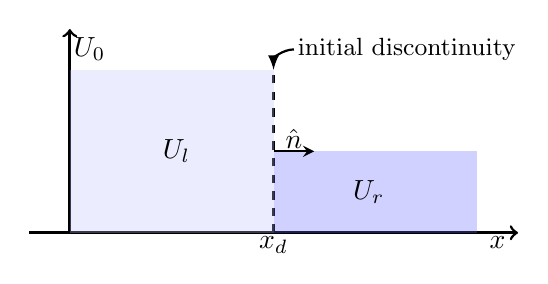
\begin{tikzpicture}[scale = {0.015\linewidth},inner sep = 1pt]

% create axis
%% \draw[->,line width=1pt] (0,0.5) |- (0.60,0) node[below]{$x$};
\draw[line width=1pt] (-0.5,0.45) node[right]{$\mbf{U}_0$}|-(0.55,0) node[below]{$x$};
\draw[->,line width=1pt] (0.55,0)--(0.6,0);
\draw[->,line width=1pt] (-0.5,0.45)--(-0.5,0.5);
\draw[line width=1pt] (-0,0)--(-0.6,0);  

% discontinuity
\draw[dashed,line width=1pt] (0,0) node[below]{$x_d$} -- (0,0.4); 
%% \draw[<-,line width=1pt] (-0.60,0) -- (0,0); 
\draw[-latex,thick](0.05,0.45)node[right]{\small initial discontinuity}
         to[out=180,in=90] (0,0.4);

% initial states
\fill[blue!25!,opacity=.3] (-0.5,0) rectangle (0,0.4);
\fill[blue!60!,opacity=.3] (0,0) rectangle (0.5,0.2);
\node[right] at (-0.28,0.2) {$\mbf{U}_l$};
\node[left] at (0.28,0.1) {$\mbf{U}_r$};


% normal
%% \draw[-stealth,thick] (0,0.25) -- (0.1,0.25); 
%% \node[] at (0.05,0.28) {$\hat{n}$};
\draw[-stealth,thick] (0,0.2) -- (0.1,0.2); 
\node[] at (0.05,0.23) {$\hat{n}$};

\end{tikzpicture}


%-----------------------------------------------------------------
% Shocktube 2D
%-----------------------------------------------------------------
%% \begin{tikzpicture}[scale = {0.015\linewidth},inner sep = 1pt]
%% % create axis
%% \draw[<->,line width=1pt] (0,0.6) node[right]{$y$} |- (1.1,0) node[below]{$x$};
%% %% \draw[<-,line width=1pt] (-0.75,0) -- (0,0); 

%% %% % normal
%% %% \draw[-stealth,thick] (0,0.25) -- (0.1,0.25); 
%% %% \node[] at (0.05,0.28) {$\hat{n}$};

%% % initial states
%% \draw[fill=blue!25!,opacity=.3] (0,0) -- (0,0.5) -- (1.0,0) -- cycle;
%% \draw[fill=blue!60!,opacity=.3] (0,0.5) -- (1.0,0.5) -- (1.0,0) -- cycle;
%% \node[right] at (0.2,0.15) {$\mbf{U}_0$};
%% \node[left] at (0.8,0.35) {$\mbf{U}_1$};

%% % discontinuity
%% \draw[line width = 1pt] (0,0.5) -- (1.0,0);
%% \draw[-latex,thick](0.2,0.55)node[right]{\small initial discontinuity}
%%          to[out=180,in=90] (0.1,0.45);

%% % normal
%% \draw[-stealth,thick] (0.5,0.25) -- (0.55,0.35); 
%% \node[] at (0.55,0.29) {$\hat{n}$};

%% \end{tikzpicture}

\end{center}
\caption{Initial conditions for a one-dimensional Riemann problem.  The initial discontinuity at, $x_d$, separates two constant states, $\mbf{U}_l$ and $\mbf{U}_r$.}
\label{fig:ivp}
\end{figure}

Conservation laws are a system of partial differential equations of the form   
\begin{gather*}
\pdbf{U}{t} + \pdbf{F}{\mbf{x}} = \mbf{0} \text{ ,}
\end{gather*} 
where \mbf{U} is a vector of the conservative state variables and \mbf{F} is a vector of fluxes \citep{Toro:1999}. 


%-----------------------------------------------------------------
% Linear advection
%-----------------------------------------------------------------
\section[Linear advection]{Linear advection}
\label{sec:lin_advec}

The one-dimensional linear advection equation is 
\begin{gather}
\label{eqn:linear_ad}
\pd{u}{t} + a\pd{u}{x} = 0,
\end{gather}
where $u$ is the conserved variable, and  $a$ is the constant wave velocity.  The solution to the Riemann problem for linear advection with $a>0$, initial conditions given by Equation~\ref{eqn:lin_ad_ivp}, and $x_d = 0$ is   
\begin{gather*}
\label{eqn:lin_ad_ivp} 
u = 
\begin{cases}
u_l & \text{if}\;\;\; x < at, \\
u_r & \text{if}\;\;\; x > at. \\
\end{cases}
\end{gather*} 

%-----------------------------------------------------------------
% Linear advection Riemann states
%-----------------------------------------------------------------
\begin{figure}[htbp]
\begin{center}
\tikzsetnextfilename{lin_ad_rstates}
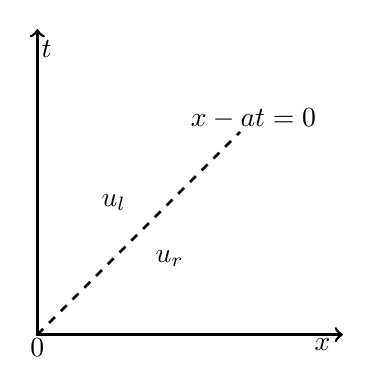
\begin{tikzpicture}[scale = {0.015\linewidth},inner sep = 1pt]
%% \begin{tikzpicture}[scale = {0.015\linewidth},inner sep = 1pt]
%% \tikzstyle{every node} = [draw,circle,fill=gray!30];
%% \draw (-1.5,0.0) circle (0.8);
%% \draw[<->,line width=1pt] (0,1) node[right]{\;$t$}|-(1,0) node[below]{$m$};

\draw[line width=1pt] (0.0,0.7) node[right]{$t$}|-(0.7,0) node[below]{$x$};
\draw[->,line width=1pt] (0.7,0)--(0.75,0);
\draw[->,line width=1pt] (0.0,0.7)--(0.0,0.75);

\node[draw=white] (char) at (0.53033,0.53033) {$x - at = 0$};
\draw[dashed,line width=1pt] (0,0) node[below]{$0$} -- (char); 

\node[draw=white] at (0.18750,0.32476) {$u_l$};
\node[draw=white] at (0.32476,0.18750) {$u_r$};

\end{tikzpicture}

\end{center}
\caption{Solution to the Riemann problem for linear advection in the $x$-$t$ plane.  The position of the discontinuity is given by the dashed line.}
\label{fig:lin_ad_rstates}
\end{figure}

In the $x$-$t$ plane, the solution changes from the initial left state, $u_l$, to the initial right state, $u_r$, across the characteristic line $x - at = 0$.  Across the discontinuity the solution is given by the Rankine-Hugonoit jump conditions, which express the transition as conservation across the discontinuity:
\begin{gather}
\label{eqn:rh_jump}
\mbf{F}_r - \mbf{F}_l = S_i (\mbf{U}_r - \mbf{U}_l),
\end{gather}      
where $S_i$ is the speed of a discontinuity connecting two states $\mbf{U}_l$ and $\mbf{U}_l$.  For the linear advection equation, the jump conditions are
\begin{gather*}
a u_r - a u_l = S (u_r - u_l),
\end{gather*}      
which gives the wave speed $S = a$.  This is the speed defined by the characteristic, $x - at = 0$.

%-----------------------------------------------------------------
% Linear systems
%-----------------------------------------------------------------
\section[Linear systems]{Linear systems}
\label{sec:lin_sys}

Consider the hyperbolic system of $n$ linear equations
\begin{gather}
\label{eqn:linear_sys}
\pdbf{U}{t} + \mbf{A}\pdbf{U}{x} = 0,
\end{gather}
where $\mbf{A}$ is an $n \times n$ constant coefficient matrix.  If $\mbf{A}$ has $n$ real eigenvalues, $\lambda_1, \hdots, \lambda_n$, and a corresponding set of $n$ linearly independent right eigenvectors, $\mbf{r}^1,\hdots,\mbf{r}^n$, the system is called hyperbolic.  It is called strictly hyperbolic system if the eigenvalues are distinct.  The hyperbolicity of the systems allows for it to be written in terms of the characteristic variables, that are the components of $\mbf{W} = \mbf{l}^i \mbf{U}$, where $\mbf{l}^i$ is the matrix of left eigenvectors, see \citep{Toro:1999}.  In characteristic form, the system is 
\begin{gather}
\pdbf{W}{t} + \mbf{\Lambda} \pdbf{W}{x} = 0,
\end{gather}  
where $\mbf{\Lambda}$ is a diagonal matrix and  $i$-th entry of the main diagonal is $\lambda_i$.
The system has been transformed to $n$ scalar equations of the form
\begin{gather}
\pd{w_i}{t} + \lambda_i \pd{w_i}{x} = 0,
\end{gather}  
where the eigenvalues are the characteristic speeds.  The system is assumed to be strictly hyperbolic so that eigenvalues are arranged such that ${\lambda_1 < \hdots < \lambda_i < \hdots < \lambda_n}$.  The solution to each scalar equation is given in terms of the characteristic variables by the solution to a linear advection problem with $a = \lambda_i$. 

%-----------------------------------------------------------------
% Linear system Riemann states
%-----------------------------------------------------------------
\begin{figure}[htbp]
\begin{center}
\tikzsetnextfilename{lin_sys_rstates}
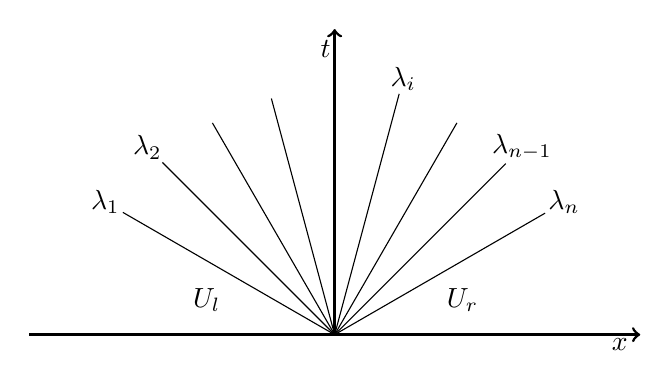
\begin{tikzpicture}[scale = {0.015\linewidth},inner sep = 1pt]
%% \begin{tikzpicture}[scale = {0.015\linewidth},inner sep = 1pt]
%% \tikzstyle{every node} = [draw,circle,fill=gray!30];
%% \draw (-1.5,0.0) circle (0.8);
%% \draw[<->,line width=1pt] (0,1) node[right]{\;$t$}|-(1,0) node[below]{$m$};
\draw[line width=1pt] (0,0.7) node[left]{$t$}|-(0.7,0) node[below]{$x$};
\draw[->,line width=1pt] (0.7,0)--(0.75,0);
\draw[->,line width=1pt] (0,0.7)--(0,0.75);  
\draw[line width=1pt] (0,0)--(-0.75,0);


\node[draw=white] (w1) at (-0.56292,0.32500) {$\lambda_1$};
\node[draw=white] (w2) at (-0.45962,0.45962) {$\lambda_2$};
\node[draw=white] (wi) at (0.16823,0.62785) {$\lambda_i$};
\node[draw=white] (w5) at (0.45962,0.45962) {$\lambda_{n-1}$};
\node[draw=white] (w6) at (0.56292,0.32500) {$\lambda_n$};

\node[draw=white] (ul) at (-0.31393,0.084116) {$\mbf{U}_l$};
\node[draw=white] (ur) at (0.31393,0.084116) {$\mbf{U}_r$};

%% \node[draw=white] (R8a) at (0.53943,0.10730) {\small $\mathrm{R}$8};
%% \node[draw=white] (R7a) at (0.45731,0.30556) {\small $\mathrm{R}$7};
%% \node[draw=white] (R6a) at (0.30556,0.45731) {\small $\mathrm{R}$6};
%% \node[draw=white] (R5a) at (0.10730,0.53943) {\small $\mathrm{R}$5};
%% \node[draw=white] (R4a) at (-0.10730,0.53943) {\small $\mathrm{R}$4};
%% \node[draw=white] (R3a) at (-0.30556,0.45731) {\small $\mathrm{R}$3};
%% \node[draw=white] (R2a) at (-0.45731,0.30556) {\small $\mathrm{R}$2};
%% \node[draw=white] (R1a) at (-0.53943,0.10730) {\small $\mathrm{R}$1};

%% \node[] at (0.15,0.95) {contact};
\draw (0,0) -- (w1);  
\draw (0,0) -- (w2);  
\draw (0,0) -- (-0.30000,0.51962);%(w3);  
\draw (0,0) -- (-0.15529,0.57956);
\draw (0,0) -- (wi);  
\draw (0,0) -- (0.30000,0.51962);%(w4);  
\draw (0,0) -- (w5);  
\draw (0,0) -- (w6);  
\end{tikzpicture}

\end{center}
\caption{Solution to the Riemann problem for a hyperbolic system of $n$ linear equations in the $x$-$t$ plane.}
\label{fig:lin_sys_rstates}
\end{figure}

The solution in the $x$-$t$ plane, for the linear system is shown in Figure~\ref{fig:lin_sys_rstates}.  It is composed of $n$ waves, each one corresponding to a characteristic speed, propagating away from the initial discontinuity.  Only the state on one side of the wave is needed to determine the change across it because the speed of a linear wave is independent of the discontinuous quantity.  The speed of the wave is calculated by the quantities in the known state.  A rotational discontinuity is an example of a linear wave in plasma physics.  It travels with a velocity equal to the Alf{\'e}n velocity, $B_n/\sqrt{4\pi\rho}$, where $B_n$ is the magnitude of the normal component of the magnetic field, and $\rho$ is the density.  Across a rotational discontinuity, $B_n$, and $\rho$ are unchanged, and determine the speed, and the jump conditions are then used to compute the connected state.  In this way, every state, connected through multiple waves can be determined.  The complete solution is then given by the superposition of the $n$ waves.  

The difference in characteristic variables across each wave is given by $\alpha_i = \mbf{l}_i \cdot (\mbf{U}_l - \mbf{U}_r)$, and the solution in terms of conservative variables is 
\begin{gather*} 
\mbf{U} = \mbf{U}_l + \sum_{i=1}^m \alpha_i \mbf{r}^i, \;\;\;\;\text{ or }\;\;\;\; \mbf{U} = \mbf{U}_r - \sum_{i=m+1}^n \alpha_i \mbf{r}^i,
\end{gather*} 
for $\lambda_m < x/t < \lambda_{m+1}$.  As described next section, the states on both sides of a nonlinear wave are needed to determine the speed.  As such, only local knowledge of the solution is available at a nonlinear discontinuity.

%-----------------------------------------------------------------
% Nonlinear systems
%-----------------------------------------------------------------
\section[Nonlinear systems]{Nonlinear systems}
\label{sec:nonlin_sys}

The results from the previous sections are now extended to nonlinear hyperbolic systems of the form   
\begin{gather}
\label{eqn:nonlinear_sys}
\pdbf{U}{t} + \pdbf{F}{x} = 0,
\end{gather}
where $\mbf{U}$ is a vector of conserved variables and $\mbf{F}(\mbf{U})$ is the flux vector.  The system is called hyperbolic if the Jacobian matrix, $\mbf{J}(\mbf{U}) = \partial{\mbf{F}}/\partial{\mbf{U}}$, has $n$ real eigenvalues and a corresponding set of $n$ linearly independent right eigenvectors.  Again the The system is also assumed to be strictly-hyperbolic so that the eigenvalues can be cosidered ordered based on speed.  For each of the $n$ eigenvalues there is an associated wave with speed $S_i$.  As with the linear system, the $n$ waves partition the solution into $n+1$ states.  Each wave in the linear system travels at a constant speed, $\lambda_i$, and has an associated jump discontinuity.  In the nonlinear systems, the wave speeds are functions of the conservative variables and the structure of the wave is not always a jump discontinuity.

%-----------------------------------------------------------------
% Characteristics of shocks, linear waves, and rarefactions
%-----------------------------------------------------------------
\begin{figure}[htbp]
\begin{tabular}{ccc}
\resizebox{0.33\linewidth}{!}{\tikzsetnextfilename{shock_char}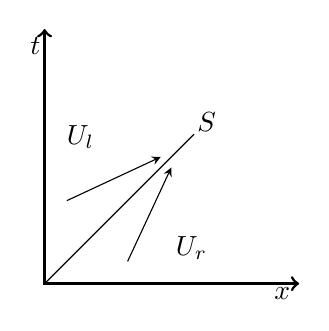
\begin{tikzpicture}[scale = {0.0125\linewidth},inner sep = 1pt]

\draw[line width=1pt] (0,0.7) node[left]{$t$}|-(0.7,0) node[below]{$x$};
\draw[->,line width=1pt] (0.7,0)--(0.75,0);
\draw[->,line width=1pt] (0,0.7)--(0,0.75);  

\node[draw=white] (sr) at (0.47730,0.47730) {$S$};

\node[draw=white] (usl) at (0.10589,0.43273) {$\mbf{U}_{l}$};
\node[draw=white] (ul) at (0.43273,0.10589) {$\mbf{U}_{r}$};

\draw (0,0) -- (sr);  

\draw[->,>=stealth] (0.24450,0.065514) -- (0.37325,0.34202);  
\draw[->,>=stealth] (0.065514,0.24450) -- (0.34202,0.37325);  

\end{tikzpicture}
} &
\resizebox{0.33\linewidth}{!}{\tikzsetnextfilename{linear_char}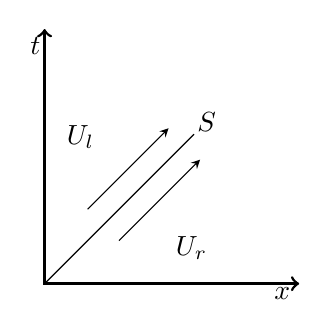
\begin{tikzpicture}[scale = {0.0125\linewidth},inner sep = 1pt]

\draw[line width=1pt] (0,0.7) node[left]{$t$}|-(0.7,0) node[below]{$x$};
\draw[->,line width=1pt] (0.7,0)--(0.75,0);
\draw[->,line width=1pt] (0,0.7)--(0,0.75);  

\node[draw=white] (sr) at (0.47730,0.47730) {$S$};

\node[draw=white] (usl) at (0.10589,0.43273) {$\mbf{U}_{l}$};
\node[draw=white] (ul) at (0.43273,0.10589) {$\mbf{U}_{r}$};

\draw (0,0) -- (sr);  

\draw[->,>=stealth] (0.21921,0.12656) -- (0.45786,0.36521);  
\draw[->,>=stealth] (0.12656,0.21921) -- (0.36521,0.45786);  

\end{tikzpicture}
} &
\resizebox{0.33\linewidth}{!}{\tikzsetnextfilename{rarefaction_char}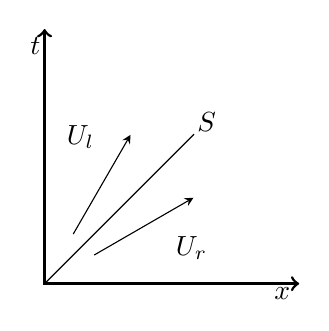
\begin{tikzpicture}[scale = {0.0125\linewidth},inner sep = 1pt]

\draw[line width=1pt] (0,0.7) node[left]{$t$}|-(0.7,0) node[below]{$x$};
\draw[->,line width=1pt] (0.7,0)--(0.75,0);
\draw[->,line width=1pt] (0,0.7)--(0,0.75);  

\node[draw=white] (sr) at (0.47730,0.47730) {$S$};

\node[draw=white] (usl) at (0.10589,0.43273) {$\mbf{U}_{l}$};
\node[draw=white] (ul) at (0.43273,0.10589) {$\mbf{U}_{r}$};

\draw (0,0) -- (sr);  

\draw[->,>=stealth] (0.14614,0.084376) -- (0.43843,0.25313);  
\draw[->,>=stealth] (0.084376,0.14614) -- (0.25313,0.43843);  

\end{tikzpicture}
} 
\end{tabular}
\caption{(left) Characteristics on both sides of a shock, (center) linear discontinuity, and (right) rarefaction (right).}
\label{fig:nonlinear_char}
\end{figure}

The formation of compression and expansion waves is an distinguishing feature of nonlinear systems.  Shock waves are compressive discontinuities that connect two states.  The characteristics of the two states connected by shock wave converge in the $x$-$t$ planeas shown in the left panel of Figure~\ref{fig:nonlinear_char}..  The Rankine-Hugonoit jump conditions for a shock wave are given by Equation~\ref{eqn:rh_jump}.

Expansion shocks are possible solutions, however, they violate the entropy condition and are disregarded as unphysical.  The entropy is defined, $p_g/\rho^{\gamma}$, where $p_g$ is the gas pressure, $\rho$ is the density, and $\gamma$ is the ratio of specific heats.  The entropy condition states that the entropy cannot decrease across a shock.    

Rarefactions are another nonlinear wave.  They connect two states through a smooth transition.  Unlike shocks, they are an expansion wave, and the characteristics of two states connected by rarefaction wave diverge in the $x$-$t$ plane, as shown in the right panel of Figure~\ref{fig:nonlinear_char}.

We adopt the following conventions when discussing to the structure of the solution to Riemann problems.  For a wave propagating with speed $S$, connecting two constant states, the upstream state, $\mbf{U}_u$, is the pre-shock state, i.e., the state of the flow that has not crossed the shock.  The downstream state, $\mbf{U}_d$, is the post-shock state, i.e., the state of the flow that has crossed the shock.  For the right-going wave shown in Figure~\ref{fig:ivp}, $\mbf{U}_l$ the upstream state, and $\mbf{U}_r$ is the downstream state.  The difference across a discontinuity is denoted with square brackets, e.g., $[ \mbf{U} ] = \mbf{U}_d - \mbf{U}_u$.

%-----------------------------------------------------------------
% Intermediate Riemann state
%-----------------------------------------------------------------
\begin{figure}[htbp]
\begin{center}
\tikzsetnextfilename{inter_rstates}
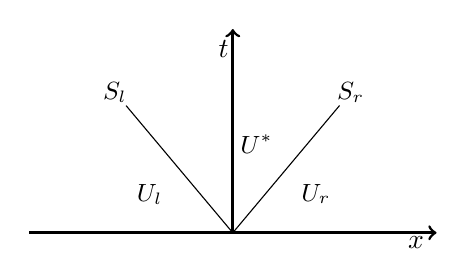
\begin{tikzpicture}[scale = {0.015\linewidth},inner sep = 1pt]
%% \begin{tikzpicture}[scale = {0.015\linewidth},inner sep = 1pt]
%% \tikzstyle{every node} = [draw,circle,fill=gray!30];
%% \draw (-1.5,0.0) circle (0.8);
%% \draw[<->,line width=1pt] (0,1) node[right]{\;$t$}|-(1,0) node[below]{$m$};
\draw[line width=1pt] (0,0.45) node[left]{$t$}|-(0.45,0) node[below]{$x$};
\draw[->,line width=1pt] (0.45,0)--(0.5,0); % extent x-axis  
\draw[->,line width=1pt] (0,0.45)--(0,0.5); % extent t-axis  
\draw[line width=1pt] (-0,0)--(-0.5,0); % draw negative x-axis  

\node[draw=white] (fr) at (-0.28925,0.34475) {\small $S_l$};
\node[draw=white] (fl) at (0.28925,0.34475) {\small $S_r$};

\node[draw=white] (Ul) at (-0.20392,0.095089) {\small $\mbf{U}_l$};
\node[draw=white] (Us) at (0.058234,0.21733) {\small $\mbf{U}^*$};
\node[draw=white] (Ur) at (0.20392,0.095089) {\small $\mbf{U}_r$};

%% \node[] at (0.15,0.95) {contact};
\draw (0,0) -- (fr);  
\draw (0,0) -- (fl);  
\end{tikzpicture}

\end{center}
\caption{Solution to a Riemann with one intermediate state in the $x$-$t$ plane.}
\label{fig:inter_rstates}
\end{figure}

When the solution to a Riemann problem is composed of more than one wave, the state between two waves is called an intermediate state, and is denoted $\mbf{U}^*$.  If the solution includes more than two waves, then the intermediate states are referenced in relation to the left-most and right-most state.  If $n+1$ states compose the solution, the states downstream of $\mbf{U}_{j}$ are denoted $\mbf{U}_{ij}^*$, where $i=1,\hdots,m/2$, $j = l,r$, and
\begin{gather*}
m = 
\begin{cases}
n & \text{if}\;\;\; n \text{ is even}, \\
n+1 & \text{if}\;\;\; n \text{ is odd}. \\
\end{cases}
\end{gather*} 
If $n$ is even, then the middle state is written without a subscript.

%-----------------------------------------------------------------
% Compressible hydrodynamics
%-----------------------------------------------------------------
\section[Compressible hydrodynamics]{Compressible hydrodynamics}
\label{sec:com_hydro}

The Euler equations of compressible hydrodynamics comprise a nonlinear hyperbolic system of conservation laws. The structure of the solution for Riemann problems of compressible hydrodynamics is presented below.  If viscosity and thermal conductivity are neglected, then the Euler equations describe the evolution of a compressible ideal gas.  The equations form a strictly-hyperbolic system that admit shocks, rarefactions, and linear discontinuities.  The conservative form of the Euler equations is
\begin{gather}
\label{eqn:euler1} \pd{\rho}{t} + \diverge{\left(\rho\mbf{v}\right)} = 0 \text{ ,} \\
\label{eqn:euler2} \pd{(\rho \mbf{v})}{t} + \diverge{\left[ \outerproduct{\rho\mbf{v}}{\mbf{v}} + p_g \right]}  = 0 \text{ ,}\\
\label{eqn:euler3} \pd{E}{t} + \diverge{\left[ \left(E + p_g \right)\mbf{v}\right]}  = 0 \text{ ,}
\end{gather}
where the energy density is defined as
\begin{gather}
  \label{eqn:energy} E = \frac{p_g}{\gamma - 1} + \frac{\rho v^2}{2}\text{ ,}
\end{gather}
$v^2 = v_n^2 + \mbf{v}_{t}^2$, and the gas constant $\gamma$ is the ratio of specific heats.  The one-dimensional quasi-linear form of the Euler equations is 
\begin{gather}
\label{eqn:euler_qlin}
\pdbf{U}{t} + \mbf{A}(\mbf{U})\pdbf{U}{x} = 0.
\end{gather}
The Jacobian of $\mbf{A}(\mbf{U})$ must have three real and distinct eigenvalues and a set of three linearly independent right eigenvectors because the system is strictly-hyperbolic.  If the eigenvalues are arranged such that $\lambda_1 < \lambda_2 < \lambda_3$, then $\lambda_1  \text{ and } \lambda_3$ correspond to nonlinear waves, and $\lambda_2$ is a linear wave.  The nonlinear waves can be either a shock (i.e., discontinuous wave) or rarefaction (i.e. smooth wave).  The linear wave is \gls{cd} that carries a carries a single jump in density and satisfies the jump conditions given by Equation~\ref{eqn:rh_jump}.  The three eigenvalues and their associated waves are:
\begin{align*}
\lambda_3 &= v_n + a : \text{fast rarefaction or shock,} \\
\lambda_2 &= v_n \phantom{+ a} : \text{contact discontinuity, \text{ and }} \\
\lambda_1 &= v_n - a : \text{slow rarefaction or shock,} 
\end{align*}
where $a = \sqrt{\gamma p_g/\rho}$ is the speed of sound.  

%-----------------------------------------------------------------
% Euler Riemann states
%-----------------------------------------------------------------
\begin{figure}[htbp]
\begin{center}
\tikzsetnextfilename{euler_rstates}
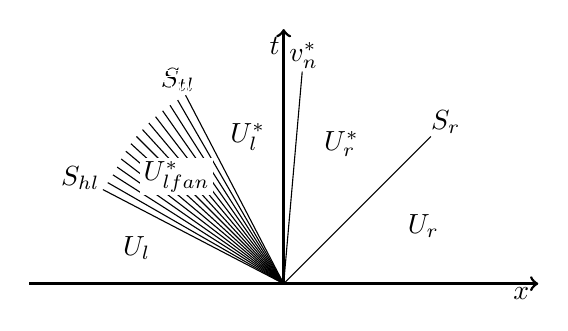
\begin{tikzpicture}[scale = {0.0125\linewidth},inner sep = 1pt]
%% \begin{tikzpicture}[scale = {0.015\linewidth},inner sep = 1pt]
%% \tikzstyle{every node} = [draw,circle,fill=gray!30];
%% \draw (-1.5,0.0) circle (0.8);
%% \draw[<->,line width=1pt] (0,1) node[right]{\;$t$}|-(1,0) node[below]{$m$};
\draw[line width=1pt] (0,0.7) node[left]{$t$}|-(0.7,0) node[below]{$x$};
\draw[->,line width=1pt] (0.7,0)--(0.75,0);
\draw[->,line width=1pt] (0,0.7)--(0,0.75);  
\draw[line width=1pt] (-0,0)--(-0.75,0);
\node[draw=white] (sr) at (0.47730,0.47730) {$S_r$};
\node[draw=white] (cd) at (0.058830,0.67243) {$v^*_n$};

\node[draw=white] (shl) at (-0.31168,0.59873) {$S_{tl}$};
\node[draw=white] (shlf) at (-0.33750,0.58457) {$\phantom{S_{tl}}$};
\node[draw=white] (shle) at (-0.36268,0.56929) {$\phantom{S_{tl}}$};
\node[draw=white] (shld) at (-0.38716,0.55293) {$\phantom{S_{tl}}$};
\node[draw=white] (shlc) at (-0.41091,0.53551) {$\phantom{S_{tl}}$};
\node[draw=white] (shlb) at (-0.43388,0.51708) {$\phantom{S_{tl}}$};
\node[draw=white] (shla) at (-0.45602,0.49766) {$\phantom{S_{tl}}$};
\node[draw=white] (sl) at (-0.47730,0.47730) {$\phantom{S_l}$};
\node[draw=white] (stla) at (-0.49766,0.45602) {$\phantom{S_{hl}}$};
\node[draw=white] (stlb) at (-0.51708,0.43388) {$\phantom{S_{hl}}$};
\node[draw=white] (stlc) at (-0.53551,0.41091) {$\phantom{S_{hl}}$};
\node[draw=white] (stld) at (-0.55293,0.38716) {$\phantom{S_{hl}}$};
\node[draw=white] (stle) at (-0.56929,0.36268) {$\phantom{S_{hl}}$};
\node[draw=white] (stlf) at (-0.58457,0.33570) {$\phantom{S_{hl}}$};
\node[draw=white] (stl) at (-0.59873,0.31168) {$S_{hl}$};

\node[draw=white] (ur) at (0.41159,0.17049) {$\mbf{U}_{r}$};
\node[draw=white] (usr) at (0.17049,0.41159) {$\mbf{U}^*_{r}$};
\node[draw=white] (usl) at (-0.10589,0.43273) {$\mbf{U}^*_{l}$};
\node[draw=white] (ul) at (-0.43273,0.10589) {$\mbf{U}_{l}$};

\draw (0,0) -- (sr);  
\draw (0,0) -- (cd);  
\draw (0,0) -- (shl);  
\draw (0,0) -- (shlf);  
\draw (0,0) -- (shle);  
\draw (0,0) -- (shld);  
\draw (0,0) -- (shlc);  
\draw (0,0) -- (shlb);  
\draw (0,0) -- (shla);  
\draw (0,0) -- (sl);  
\draw (0,0) -- (stla);  
\draw (0,0) -- (stlb);  
\draw (0,0) -- (stlc);  
\draw (0,0) -- (stld);  
\draw (0,0) -- (stle);  
\draw (0,0) -- (stlf);  
\draw (0,0) -- (stl);  

\node[draw=white,rectangle,fill=white] (usl) at (-0.31502,0.31502) {$\mbf{U}^*_{lfan}$};

\end{tikzpicture}

\end{center}
\caption{Possible structure of the solution to a Riemann problem for the Euler equations the $x$-$t$ plane.  The solution consists of a rarefaction wave to the left of contact discontinuity, and a shock wave to the right.}
\label{fig:euler_rstates}
\end{figure}

A possible structure of the self-similar solution $\mbf{U}(x,t)$ to the Euler equations is shown in Figure~\ref{fig:euler_rstates}.  Three waves: a fast shock, a contact discontinuity, and a slow rarefaction, separate the four constant states: the initial left, left intermediate, right intermediate, and initial right.  The state, $\mbf{U}^*_{lfan}$, inside the rarefaction wave is not constant.  It connects the states $\mbf{U}_l$ and $\mbf{U}^*_l$ through a smooth transition.  The characteristic speed at the head of a rarefaction wave is $v_{nu} \pm a_u$.  At the tail of a rarefaction wave, the characteristic speed is $v_{nd} \pm a_d$.  The plus (minus) sign refers to right-going (left-going) waves.  The speed of the contact discontinuity is given by the characteristic speed $\lambda_2$.  The shock speeds are derived from the Rankine-Hugonoit jump conditions, Equation~\ref{eqn:rh_jump}.  The speeds of a right-going shock, $S_r$, and left-going shock, $S_l$, are
\begin{gather*}
S_r = v_{nr} + a_r \sqrt{\left(\frac{\gamma + 1}{2\gamma}\right) \left(\frac{p_g^*}{p_{gr}}\right) + \left(\frac{\gamma - 1}{2\gamma}\right)}, \\
S_{l} = v_{nl} - a_l \sqrt{\left(\frac{\gamma + 1}{2\gamma}\right) \left(\frac{p_g^*}{p_{gl}}\right) + \left(\frac{\gamma - 1}{2\gamma}\right)},
\end{gather*}
where $p^*_{g} = p^*_{gl} = p^*_{gr}$, since the gas pressure is unchanged across a contact discontinuity.  The velocity at the head (tail) of a rarefaction wave is given by the corresponding characteristic speed in the upstream (downstream) state.  

%-----------------------------------------------------------------
% Riemann solvers
%-----------------------------------------------------------------
\subsection[Exact Riemann solvers]{Exact Riemann solver}
\label{sec:hydro_exact_rsolvers}

The solution to a Riemann problem consists of $n$ waves separating $n+1$ states, and it is found by determining the speed of each wave, and the jump associated with each wave.  Solving a Riemann problem for the one-dimensional Euler equations requires determining two unknown states, $\mbf{U}^*_l$ and $\mbf{U}^*_l$, and three wave speeds.  The exact solution is calculated by improving an initial guess for gas pressure in the intermediate states through an iterative procedure, e.g., Newton's method \citep{Toro:1999}.  The iteration is carried out until the jump condition for the normal velocity at the contact discontinuity, $[v^*_n] = 0$, is satisfied to the desired accuracy.  In practice, this is done by finding the root of the equation
\begin{gather*}
f(p^*_g,\mbf{U}_l,\mbf{U}_r) \equiv f_r(p_{gr},\mbf{U}_r) + f_l(p_{gl},\mbf{U}_l) + v_{nr} - v_{nl} = 0 \, ,
\end{gather*}
where $f_r$ ($f_l$) is a function connecting the initial right (left) state to the intermediate right (left) state.  The normal velocity in the intermediate states (Equation (4.9) of \citep{Toro:1999}) is 
\begin{gather*}
v^*_n = \half (v_{nr} + v_{nl}) + \half (f_r - f_l).
\end{gather*}
The functions $f_l$ and $f_r$ depend on the type of wave, i.e. shock or rarefaction.  If pressure increases across the wave, $p^*_d > p_{gu}$, then the wave is a shock, otherwise, the wave is a rarefaction.  The function $f_j$, for $j=l$ and $j=r$, (Equations (4.6) and (4.7) of \citep{Toro:1999}) is given by
\begin{gather*}
f_j(p_{gj},\mbf{U}_j) = 
\begin{cases}
(p^*_g - p_{gj})\left[ \frac{2}{\rho_j((\gamma +1)p^*_{g} + (\gamma -1)p_{gl})} \right]^{\half} 
  %% \phantom{\frac{2a_j}{(p^*_g - 1)}\left[\left(\frac{p^*_g}{p_{gj}} \right)^{\frac{\gamma-1}{2\gamma}} - 1\right]} 
  \;\;\;\; \text{if}\;\;\; p^*_g > p_{gj}, \\
\frac{2a_j}{(p^*_g - 1)}\left[\left(\frac{p^*_g}{p_{gj}} \right)^{\frac{\gamma-1}{2\gamma}} - 1\right] 
  %% \phantom{(p^*_g - p_{gj})\left[ \frac{2}{\rho_j((\gamma +1)p^*_{g} + (\gamma -1)p_{gl})} \right]^{\half}} 
  \;\;\;\;\;\;\;\;\;\;\;\;\;\;\;\;\;\;\;\; \text{if}\;\;\; p^*_g \le p_{gj}. \\
\end{cases}
\end{gather*}
where $j=l$ and $j=r$.  The densities $\rho_j$ for $j=l$ and $r$, in the left and right intermediate states are
\begin{gather*}
\rho^*_j = 
\begin{cases}
\rho_j\left[ \frac{\frac{p^*_g}{p_{gj}} + \frac{\gamma-1}{\gamma+1}}
  {\frac{\gamma-1}{\gamma+1} \frac{p^*_g}{p_{gj}} + 1} \right] 
  \;\;\;\; \text{if}\;\;\; p^*_g > p_{gj}, \\
\rho_j\left( \frac{p^*_g}{p_{gj}} \right)^{\frac{1}{\gamma}}
  \;\;\;\;\;\;\;\;\;\;\; \text{if}\;\;\; p^*_g \le p_{gj}. \\
\end{cases}
\end{gather*}
If the solution contains a rarefaction wave then the states in the fan are needed to complete the solution.  The state in the rarefaction wave is  
\begin{gather*}
\rho = \rho_j \left[ \frac{2}{(\gamma+1)} \pm \frac{(\gamma-1)}{(\gamma+1)a_j}
  \left(v_{nj} - \frac{x}{t}\right)\right]^{\frac{2}{\gamma - 1}}, \\
v_{n} = \frac{2}{(\gamma+1)} \left[\frac{(\gamma-1)}{2}v_{nj} \pm a_j + \frac{x}{t}\right], \\ 
p_{g} = p_{gj} \left[ \frac{2}{(\gamma+1)} \pm \frac{(\gamma-1)}{(\gamma+1)a_j}
  \left(v_{nj} - \frac{x}{t}\right)\right]^{\frac{2\gamma}{\gamma - 1}}, 
\end{gather*}
for $j=l$ and $r$, and the plus (minus) sign corresponds to a left-going (right-going) wave.

%-----------------------------------------------------------------
% Exact solution to Sod shock tube
%-----------------------------------------------------------------
\begin{figure}[htbp]
\begin{tabular}{ccc}
\resizebox{0.33\linewidth}{!}{\tikzsetnextfilename{sod_1}\begin{tikzpicture}[gnuplot]
%% generated with GNUPLOT 4.6p4 (Lua 5.1; terminal rev. 99, script rev. 100)
%% Sat 28 Jun 2014 11:52:07 AM EDT
\path (0.000,0.000) rectangle (8.000,6.000);
\gpfill{rgb color={1.000,1.000,1.000}} (1.012,0.985)--(7.446,0.985)--(7.446,5.630)--(1.012,5.630)--cycle;
\gpcolor{color=gp lt color border}
\gpsetlinetype{gp lt border}
\gpsetlinewidth{1.00}
\draw[gp path] (1.012,0.985)--(1.012,5.630)--(7.446,5.630)--(7.446,0.985)--cycle;
\gpcolor{color=gp lt color axes}
\gpsetlinetype{gp lt axes}
\gpsetlinewidth{2.00}
\draw[gp path] (1.012,0.985)--(7.447,0.985);
\gpcolor{color=gp lt color border}
\gpsetlinetype{gp lt border}
\draw[gp path] (1.012,0.985)--(1.084,0.985);
\draw[gp path] (7.447,0.985)--(7.375,0.985);
\gpcolor{rgb color={0.000,0.000,0.000}}
\node[gp node right,font={\fontsize{10pt}{12pt}\selectfont}] at (0.828,0.985) {0};
\gpcolor{color=gp lt color axes}
\gpsetlinetype{gp lt axes}
\draw[gp path] (1.012,1.830)--(7.447,1.830);
\gpcolor{color=gp lt color border}
\gpsetlinetype{gp lt border}
\draw[gp path] (1.012,1.830)--(1.084,1.830);
\draw[gp path] (7.447,1.830)--(7.375,1.830);
\gpcolor{rgb color={0.000,0.000,0.000}}
\node[gp node right,font={\fontsize{10pt}{12pt}\selectfont}] at (0.828,1.830) {0.2};
\gpcolor{color=gp lt color axes}
\gpsetlinetype{gp lt axes}
\draw[gp path] (1.012,2.674)--(7.447,2.674);
\gpcolor{color=gp lt color border}
\gpsetlinetype{gp lt border}
\draw[gp path] (1.012,2.674)--(1.084,2.674);
\draw[gp path] (7.447,2.674)--(7.375,2.674);
\gpcolor{rgb color={0.000,0.000,0.000}}
\node[gp node right,font={\fontsize{10pt}{12pt}\selectfont}] at (0.828,2.674) {0.4};
\gpcolor{color=gp lt color axes}
\gpsetlinetype{gp lt axes}
\draw[gp path] (1.012,3.519)--(7.447,3.519);
\gpcolor{color=gp lt color border}
\gpsetlinetype{gp lt border}
\draw[gp path] (1.012,3.519)--(1.084,3.519);
\draw[gp path] (7.447,3.519)--(7.375,3.519);
\gpcolor{rgb color={0.000,0.000,0.000}}
\node[gp node right,font={\fontsize{10pt}{12pt}\selectfont}] at (0.828,3.519) {0.6};
\gpcolor{color=gp lt color axes}
\gpsetlinetype{gp lt axes}
\draw[gp path] (1.012,4.364)--(7.447,4.364);
\gpcolor{color=gp lt color border}
\gpsetlinetype{gp lt border}
\draw[gp path] (1.012,4.364)--(1.084,4.364);
\draw[gp path] (7.447,4.364)--(7.375,4.364);
\gpcolor{rgb color={0.000,0.000,0.000}}
\node[gp node right,font={\fontsize{10pt}{12pt}\selectfont}] at (0.828,4.364) {0.8};
\gpcolor{color=gp lt color axes}
\gpsetlinetype{gp lt axes}
\draw[gp path] (1.012,5.209)--(7.447,5.209);
\gpcolor{color=gp lt color border}
\gpsetlinetype{gp lt border}
\draw[gp path] (1.012,5.209)--(1.084,5.209);
\draw[gp path] (7.447,5.209)--(7.375,5.209);
\gpcolor{rgb color={0.000,0.000,0.000}}
\node[gp node right,font={\fontsize{10pt}{12pt}\selectfont}] at (0.828,5.209) {1};
\gpcolor{color=gp lt color axes}
\gpsetlinetype{gp lt axes}
\draw[gp path] (1.012,0.985)--(1.012,5.631);
\gpcolor{color=gp lt color border}
\gpsetlinetype{gp lt border}
\draw[gp path] (1.012,0.985)--(1.012,1.057);
\draw[gp path] (1.012,5.631)--(1.012,5.559);
\gpcolor{rgb color={0.000,0.000,0.000}}
\node[gp node center,font={\fontsize{10pt}{12pt}\selectfont}] at (1.012,0.677) {0};
\gpcolor{color=gp lt color axes}
\gpsetlinetype{gp lt axes}
\draw[gp path] (2.299,0.985)--(2.299,5.631);
\gpcolor{color=gp lt color border}
\gpsetlinetype{gp lt border}
\draw[gp path] (2.299,0.985)--(2.299,1.057);
\draw[gp path] (2.299,5.631)--(2.299,5.559);
\gpcolor{rgb color={0.000,0.000,0.000}}
\node[gp node center,font={\fontsize{10pt}{12pt}\selectfont}] at (2.299,0.677) {0.2};
\gpcolor{color=gp lt color axes}
\gpsetlinetype{gp lt axes}
\draw[gp path] (3.586,0.985)--(3.586,5.631);
\gpcolor{color=gp lt color border}
\gpsetlinetype{gp lt border}
\draw[gp path] (3.586,0.985)--(3.586,1.057);
\draw[gp path] (3.586,5.631)--(3.586,5.559);
\gpcolor{rgb color={0.000,0.000,0.000}}
\node[gp node center,font={\fontsize{10pt}{12pt}\selectfont}] at (3.586,0.677) {0.4};
\gpcolor{color=gp lt color axes}
\gpsetlinetype{gp lt axes}
\draw[gp path] (4.873,0.985)--(4.873,5.631);
\gpcolor{color=gp lt color border}
\gpsetlinetype{gp lt border}
\draw[gp path] (4.873,0.985)--(4.873,1.057);
\draw[gp path] (4.873,5.631)--(4.873,5.559);
\gpcolor{rgb color={0.000,0.000,0.000}}
\node[gp node center,font={\fontsize{10pt}{12pt}\selectfont}] at (4.873,0.677) {0.6};
\gpcolor{color=gp lt color axes}
\gpsetlinetype{gp lt axes}
\draw[gp path] (6.160,0.985)--(6.160,5.631);
\gpcolor{color=gp lt color border}
\gpsetlinetype{gp lt border}
\draw[gp path] (6.160,0.985)--(6.160,1.057);
\draw[gp path] (6.160,5.631)--(6.160,5.559);
\gpcolor{rgb color={0.000,0.000,0.000}}
\node[gp node center,font={\fontsize{10pt}{12pt}\selectfont}] at (6.160,0.677) {0.8};
\gpcolor{color=gp lt color axes}
\gpsetlinetype{gp lt axes}
\draw[gp path] (7.447,0.985)--(7.447,5.631);
\gpcolor{color=gp lt color border}
\gpsetlinetype{gp lt border}
\draw[gp path] (7.447,0.985)--(7.447,1.057);
\draw[gp path] (7.447,5.631)--(7.447,5.559);
\gpcolor{rgb color={0.000,0.000,0.000}}
\node[gp node center,font={\fontsize{10pt}{12pt}\selectfont}] at (7.447,0.677) {1};
\gpcolor{color=gp lt color border}
\draw[gp path] (1.012,5.631)--(1.012,0.985)--(7.447,0.985)--(7.447,5.631)--cycle;
\gpcolor{rgb color={0.000,0.000,0.000}}
\node[gp node center,font={\fontsize{10pt}{12pt}\selectfont}] at (4.229,0.215) {\huge $x$};
\gpsetlinetype{gp lt plot 0}
\gpsetlinewidth{4.00}
\draw[gp path] (1.025,5.209)--(1.050,5.209)--(1.075,5.209)--(1.100,5.209)--(1.125,5.209)%
  --(1.150,5.209)--(1.175,5.209)--(1.201,5.209)--(1.226,5.209)--(1.251,5.209)--(1.276,5.209)%
  --(1.301,5.209)--(1.326,5.209)--(1.351,5.209)--(1.376,5.209)--(1.402,5.209)--(1.427,5.209)%
  --(1.452,5.209)--(1.477,5.209)--(1.502,5.209)--(1.527,5.209)--(1.552,5.209)--(1.578,5.209)%
  --(1.603,5.209)--(1.628,5.209)--(1.653,5.209)--(1.678,5.209)--(1.703,5.209)--(1.728,5.209)%
  --(1.754,5.209)--(1.779,5.209)--(1.804,5.209)--(1.829,5.209)--(1.854,5.209)--(1.879,5.209)%
  --(1.904,5.209)--(1.929,5.209)--(1.955,5.209)--(1.980,5.209)--(2.005,5.209)--(2.030,5.209)%
  --(2.055,5.209)--(2.080,5.209)--(2.105,5.209)--(2.131,5.209)--(2.156,5.209)--(2.181,5.209)%
  --(2.206,5.209)--(2.231,5.209)--(2.256,5.209)--(2.281,5.209)--(2.307,5.209)--(2.332,5.198)%
  --(2.357,5.152)--(2.382,5.106)--(2.407,5.061)--(2.432,5.016)--(2.457,4.971)--(2.482,4.927)%
  --(2.508,4.883)--(2.533,4.840)--(2.558,4.797)--(2.583,4.754)--(2.608,4.712)--(2.633,4.670)%
  --(2.658,4.629)--(2.684,4.588)--(2.709,4.547)--(2.734,4.506)--(2.759,4.466)--(2.784,4.427)%
  --(2.809,4.388)--(2.834,4.349)--(2.860,4.310)--(2.885,4.272)--(2.910,4.234)--(2.935,4.196)%
  --(2.960,4.159)--(2.985,4.123)--(3.010,4.086)--(3.036,4.050)--(3.061,4.014)--(3.086,3.979)%
  --(3.111,3.944)--(3.136,3.909)--(3.161,3.874)--(3.186,3.840)--(3.211,3.806)--(3.237,3.773)%
  --(3.262,3.740)--(3.287,3.707)--(3.312,3.674)--(3.337,3.642)--(3.362,3.610)--(3.387,3.578)%
  --(3.413,3.547)--(3.438,3.516)--(3.463,3.485)--(3.488,3.455)--(3.513,3.425)--(3.538,3.395)%
  --(3.563,3.366)--(3.589,3.336)--(3.614,3.307)--(3.639,3.279)--(3.664,3.250)--(3.689,3.222)%
  --(3.714,3.194)--(3.739,3.167)--(3.764,3.140)--(3.790,3.113)--(3.815,3.086)--(3.840,3.059)%
  --(3.865,3.033)--(3.890,3.007)--(3.915,2.982)--(3.940,2.956)--(3.966,2.931)--(3.991,2.906)%
  --(4.016,2.882)--(4.041,2.857)--(4.066,2.833)--(4.091,2.809)--(4.116,2.786)--(4.142,2.786)%
  --(4.167,2.786)--(4.192,2.786)--(4.217,2.786)--(4.242,2.786)--(4.267,2.786)--(4.292,2.786)%
  --(4.317,2.786)--(4.343,2.786)--(4.368,2.786)--(4.393,2.786)--(4.418,2.786)--(4.443,2.786)%
  --(4.468,2.786)--(4.493,2.786)--(4.519,2.786)--(4.544,2.786)--(4.569,2.786)--(4.594,2.786)%
  --(4.619,2.786)--(4.644,2.786)--(4.669,2.786)--(4.695,2.786)--(4.720,2.786)--(4.745,2.786)%
  --(4.770,2.786)--(4.795,2.786)--(4.820,2.786)--(4.845,2.786)--(4.870,2.786)--(4.896,2.786)%
  --(4.921,2.786)--(4.946,2.786)--(4.971,2.786)--(4.996,2.786)--(5.021,2.786)--(5.046,2.786)%
  --(5.072,2.786)--(5.097,2.786)--(5.122,2.786)--(5.147,2.786)--(5.172,2.786)--(5.197,2.786)%
  --(5.222,2.786)--(5.248,2.786)--(5.273,2.786)--(5.298,2.786)--(5.323,2.786)--(5.348,2.786)%
  --(5.373,2.786)--(5.398,2.786)--(5.423,2.786)--(5.449,2.786)--(5.474,2.786)--(5.499,2.786)%
  --(5.524,2.786)--(5.549,2.786)--(5.574,2.786)--(5.599,2.786)--(5.625,2.786)--(5.650,2.786)%
  --(5.675,2.786)--(5.700,2.786)--(5.725,2.107)--(5.750,2.107)--(5.775,2.107)--(5.801,2.107)%
  --(5.826,2.107)--(5.851,2.107)--(5.876,2.107)--(5.901,2.107)--(5.926,2.107)--(5.951,2.107)%
  --(5.977,2.107)--(6.002,2.107)--(6.027,2.107)--(6.052,2.107)--(6.077,2.107)--(6.102,2.107)%
  --(6.127,2.107)--(6.152,2.107)--(6.178,2.107)--(6.203,2.107)--(6.228,2.107)--(6.253,2.107)%
  --(6.278,2.107)--(6.303,2.107)--(6.328,2.107)--(6.354,2.107)--(6.379,2.107)--(6.404,2.107)%
  --(6.429,2.107)--(6.454,2.107)--(6.479,2.107)--(6.504,2.107)--(6.530,2.107)--(6.555,2.107)%
  --(6.580,2.107)--(6.605,2.107)--(6.630,2.107)--(6.655,2.107)--(6.680,2.107)--(6.705,2.107)%
  --(6.731,2.107)--(6.756,2.107)--(6.781,2.107)--(6.806,2.107)--(6.831,2.107)--(6.856,2.107)%
  --(6.881,2.107)--(6.907,2.107)--(6.932,2.107)--(6.957,2.107)--(6.982,2.107)--(7.007,2.107)%
  --(7.032,2.107)--(7.057,1.513)--(7.083,1.513)--(7.108,1.513)--(7.133,1.513)--(7.158,1.513)%
  --(7.183,1.513)--(7.208,1.513)--(7.233,1.513)--(7.258,1.513)--(7.284,1.513)--(7.309,1.513)%
  --(7.334,1.513)--(7.359,1.513)--(7.384,1.513)--(7.409,1.513)--(7.434,1.513);
\node[gp node left,font={\fontsize{10pt}{12pt}\selectfont}] at (1.334,4.575) {\huge $\rho$};
%% coordinates of the plot area
\gpdefrectangularnode{gp plot 1}{\pgfpoint{1.012cm}{0.985cm}}{\pgfpoint{7.447cm}{5.631cm}}
\end{tikzpicture}
%% gnuplot variables
} &
\resizebox{0.33\linewidth}{!}{\tikzsetnextfilename{sod_2}\begin{tikzpicture}[gnuplot]
%% generated with GNUPLOT 4.6p4 (Lua 5.1; terminal rev. 99, script rev. 100)
%% Sat 28 Jun 2014 11:52:07 AM EDT
\path (0.000,0.000) rectangle (8.000,6.000);
\gpfill{rgb color={1.000,1.000,1.000}} (1.012,0.985)--(7.446,0.985)--(7.446,5.630)--(1.012,5.630)--cycle;
\gpcolor{color=gp lt color border}
\gpsetlinetype{gp lt border}
\gpsetlinewidth{1.00}
\draw[gp path] (1.012,0.985)--(1.012,5.630)--(7.446,5.630)--(7.446,0.985)--cycle;
\gpcolor{color=gp lt color axes}
\gpsetlinetype{gp lt axes}
\gpsetlinewidth{2.00}
\draw[gp path] (1.012,1.407)--(7.447,1.407);
\gpcolor{color=gp lt color border}
\gpsetlinetype{gp lt border}
\draw[gp path] (1.012,1.407)--(1.084,1.407);
\draw[gp path] (7.447,1.407)--(7.375,1.407);
\gpcolor{rgb color={0.000,0.000,0.000}}
\node[gp node right,font={\fontsize{10pt}{12pt}\selectfont}] at (0.828,1.407) {0};
\gpcolor{color=gp lt color axes}
\gpsetlinetype{gp lt axes}
\draw[gp path] (1.012,2.252)--(7.447,2.252);
\gpcolor{color=gp lt color border}
\gpsetlinetype{gp lt border}
\draw[gp path] (1.012,2.252)--(1.084,2.252);
\draw[gp path] (7.447,2.252)--(7.375,2.252);
\gpcolor{rgb color={0.000,0.000,0.000}}
\node[gp node right,font={\fontsize{10pt}{12pt}\selectfont}] at (0.828,2.252) {0.2};
\gpcolor{color=gp lt color axes}
\gpsetlinetype{gp lt axes}
\draw[gp path] (1.012,3.097)--(7.447,3.097);
\gpcolor{color=gp lt color border}
\gpsetlinetype{gp lt border}
\draw[gp path] (1.012,3.097)--(1.084,3.097);
\draw[gp path] (7.447,3.097)--(7.375,3.097);
\gpcolor{rgb color={0.000,0.000,0.000}}
\node[gp node right,font={\fontsize{10pt}{12pt}\selectfont}] at (0.828,3.097) {0.4};
\gpcolor{color=gp lt color axes}
\gpsetlinetype{gp lt axes}
\draw[gp path] (1.012,3.942)--(7.447,3.942);
\gpcolor{color=gp lt color border}
\gpsetlinetype{gp lt border}
\draw[gp path] (1.012,3.942)--(1.084,3.942);
\draw[gp path] (7.447,3.942)--(7.375,3.942);
\gpcolor{rgb color={0.000,0.000,0.000}}
\node[gp node right,font={\fontsize{10pt}{12pt}\selectfont}] at (0.828,3.942) {0.6};
\gpcolor{color=gp lt color axes}
\gpsetlinetype{gp lt axes}
\draw[gp path] (1.012,4.786)--(7.447,4.786);
\gpcolor{color=gp lt color border}
\gpsetlinetype{gp lt border}
\draw[gp path] (1.012,4.786)--(1.084,4.786);
\draw[gp path] (7.447,4.786)--(7.375,4.786);
\gpcolor{rgb color={0.000,0.000,0.000}}
\node[gp node right,font={\fontsize{10pt}{12pt}\selectfont}] at (0.828,4.786) {0.8};
\gpcolor{color=gp lt color axes}
\gpsetlinetype{gp lt axes}
\draw[gp path] (1.012,5.631)--(7.447,5.631);
\gpcolor{color=gp lt color border}
\gpsetlinetype{gp lt border}
\draw[gp path] (1.012,5.631)--(1.084,5.631);
\draw[gp path] (7.447,5.631)--(7.375,5.631);
\gpcolor{rgb color={0.000,0.000,0.000}}
\node[gp node right,font={\fontsize{10pt}{12pt}\selectfont}] at (0.828,5.631) {1};
\gpcolor{color=gp lt color axes}
\gpsetlinetype{gp lt axes}
\draw[gp path] (1.012,0.985)--(1.012,5.631);
\gpcolor{color=gp lt color border}
\gpsetlinetype{gp lt border}
\draw[gp path] (1.012,0.985)--(1.012,1.057);
\draw[gp path] (1.012,5.631)--(1.012,5.559);
\gpcolor{rgb color={0.000,0.000,0.000}}
\node[gp node center,font={\fontsize{10pt}{12pt}\selectfont}] at (1.012,0.677) {0};
\gpcolor{color=gp lt color axes}
\gpsetlinetype{gp lt axes}
\draw[gp path] (2.299,0.985)--(2.299,5.631);
\gpcolor{color=gp lt color border}
\gpsetlinetype{gp lt border}
\draw[gp path] (2.299,0.985)--(2.299,1.057);
\draw[gp path] (2.299,5.631)--(2.299,5.559);
\gpcolor{rgb color={0.000,0.000,0.000}}
\node[gp node center,font={\fontsize{10pt}{12pt}\selectfont}] at (2.299,0.677) {0.2};
\gpcolor{color=gp lt color axes}
\gpsetlinetype{gp lt axes}
\draw[gp path] (3.586,0.985)--(3.586,5.631);
\gpcolor{color=gp lt color border}
\gpsetlinetype{gp lt border}
\draw[gp path] (3.586,0.985)--(3.586,1.057);
\draw[gp path] (3.586,5.631)--(3.586,5.559);
\gpcolor{rgb color={0.000,0.000,0.000}}
\node[gp node center,font={\fontsize{10pt}{12pt}\selectfont}] at (3.586,0.677) {0.4};
\gpcolor{color=gp lt color axes}
\gpsetlinetype{gp lt axes}
\draw[gp path] (4.873,0.985)--(4.873,5.631);
\gpcolor{color=gp lt color border}
\gpsetlinetype{gp lt border}
\draw[gp path] (4.873,0.985)--(4.873,1.057);
\draw[gp path] (4.873,5.631)--(4.873,5.559);
\gpcolor{rgb color={0.000,0.000,0.000}}
\node[gp node center,font={\fontsize{10pt}{12pt}\selectfont}] at (4.873,0.677) {0.6};
\gpcolor{color=gp lt color axes}
\gpsetlinetype{gp lt axes}
\draw[gp path] (6.160,0.985)--(6.160,5.631);
\gpcolor{color=gp lt color border}
\gpsetlinetype{gp lt border}
\draw[gp path] (6.160,0.985)--(6.160,1.057);
\draw[gp path] (6.160,5.631)--(6.160,5.559);
\gpcolor{rgb color={0.000,0.000,0.000}}
\node[gp node center,font={\fontsize{10pt}{12pt}\selectfont}] at (6.160,0.677) {0.8};
\gpcolor{color=gp lt color axes}
\gpsetlinetype{gp lt axes}
\draw[gp path] (7.447,0.985)--(7.447,5.631);
\gpcolor{color=gp lt color border}
\gpsetlinetype{gp lt border}
\draw[gp path] (7.447,0.985)--(7.447,1.057);
\draw[gp path] (7.447,5.631)--(7.447,5.559);
\gpcolor{rgb color={0.000,0.000,0.000}}
\node[gp node center,font={\fontsize{10pt}{12pt}\selectfont}] at (7.447,0.677) {1};
\gpcolor{color=gp lt color border}
\draw[gp path] (1.012,5.631)--(1.012,0.985)--(7.447,0.985)--(7.447,5.631)--cycle;
\gpcolor{rgb color={0.000,0.000,0.000}}
\node[gp node center,font={\fontsize{10pt}{12pt}\selectfont}] at (4.229,0.215) {\huge $x$};
\gpsetlinetype{gp lt plot 0}
\gpsetlinewidth{4.00}
\draw[gp path] (1.025,1.407)--(1.050,1.407)--(1.075,1.407)--(1.100,1.407)--(1.125,1.407)%
  --(1.150,1.407)--(1.175,1.407)--(1.201,1.407)--(1.226,1.407)--(1.251,1.407)--(1.276,1.407)%
  --(1.301,1.407)--(1.326,1.407)--(1.351,1.407)--(1.376,1.407)--(1.402,1.407)--(1.427,1.407)%
  --(1.452,1.407)--(1.477,1.407)--(1.502,1.407)--(1.527,1.407)--(1.552,1.407)--(1.578,1.407)%
  --(1.603,1.407)--(1.628,1.407)--(1.653,1.407)--(1.678,1.407)--(1.703,1.407)--(1.728,1.407)%
  --(1.754,1.407)--(1.779,1.407)--(1.804,1.407)--(1.829,1.407)--(1.854,1.407)--(1.879,1.407)%
  --(1.904,1.407)--(1.929,1.407)--(1.955,1.407)--(1.980,1.407)--(2.005,1.407)--(2.030,1.407)%
  --(2.055,1.407)--(2.080,1.407)--(2.105,1.407)--(2.131,1.407)--(2.156,1.407)--(2.181,1.407)%
  --(2.206,1.407)--(2.231,1.407)--(2.256,1.407)--(2.281,1.407)--(2.307,1.407)--(2.332,1.420)%
  --(2.357,1.475)--(2.382,1.530)--(2.407,1.585)--(2.432,1.640)--(2.457,1.695)--(2.482,1.750)%
  --(2.508,1.805)--(2.533,1.860)--(2.558,1.915)--(2.583,1.970)--(2.608,2.025)--(2.633,2.080)%
  --(2.658,2.135)--(2.684,2.190)--(2.709,2.245)--(2.734,2.300)--(2.759,2.355)--(2.784,2.410)%
  --(2.809,2.465)--(2.834,2.520)--(2.860,2.575)--(2.885,2.630)--(2.910,2.685)--(2.935,2.740)%
  --(2.960,2.795)--(2.985,2.850)--(3.010,2.905)--(3.036,2.960)--(3.061,3.015)--(3.086,3.070)%
  --(3.111,3.125)--(3.136,3.180)--(3.161,3.235)--(3.186,3.290)--(3.211,3.345)--(3.237,3.400)%
  --(3.262,3.455)--(3.287,3.510)--(3.312,3.565)--(3.337,3.620)--(3.362,3.675)--(3.387,3.730)%
  --(3.413,3.785)--(3.438,3.840)--(3.463,3.895)--(3.488,3.950)--(3.513,4.005)--(3.538,4.060)%
  --(3.563,4.115)--(3.589,4.170)--(3.614,4.225)--(3.639,4.280)--(3.664,4.335)--(3.689,4.390)%
  --(3.714,4.445)--(3.739,4.500)--(3.764,4.555)--(3.790,4.610)--(3.815,4.665)--(3.840,4.719)%
  --(3.865,4.774)--(3.890,4.829)--(3.915,4.884)--(3.940,4.939)--(3.966,4.994)--(3.991,5.049)%
  --(4.016,5.104)--(4.041,5.159)--(4.066,5.214)--(4.091,5.269)--(4.116,5.324)--(4.142,5.324)%
  --(4.167,5.324)--(4.192,5.324)--(4.217,5.324)--(4.242,5.324)--(4.267,5.324)--(4.292,5.324)%
  --(4.317,5.324)--(4.343,5.324)--(4.368,5.324)--(4.393,5.324)--(4.418,5.324)--(4.443,5.324)%
  --(4.468,5.324)--(4.493,5.324)--(4.519,5.324)--(4.544,5.324)--(4.569,5.324)--(4.594,5.324)%
  --(4.619,5.324)--(4.644,5.324)--(4.669,5.324)--(4.695,5.324)--(4.720,5.324)--(4.745,5.324)%
  --(4.770,5.324)--(4.795,5.324)--(4.820,5.324)--(4.845,5.324)--(4.870,5.324)--(4.896,5.324)%
  --(4.921,5.324)--(4.946,5.324)--(4.971,5.324)--(4.996,5.324)--(5.021,5.324)--(5.046,5.324)%
  --(5.072,5.324)--(5.097,5.324)--(5.122,5.324)--(5.147,5.324)--(5.172,5.324)--(5.197,5.324)%
  --(5.222,5.324)--(5.248,5.324)--(5.273,5.324)--(5.298,5.324)--(5.323,5.324)--(5.348,5.324)%
  --(5.373,5.324)--(5.398,5.324)--(5.423,5.324)--(5.449,5.324)--(5.474,5.324)--(5.499,5.324)%
  --(5.524,5.324)--(5.549,5.324)--(5.574,5.324)--(5.599,5.324)--(5.625,5.324)--(5.650,5.324)%
  --(5.675,5.324)--(5.700,5.324)--(5.725,5.324)--(5.750,5.324)--(5.775,5.324)--(5.801,5.324)%
  --(5.826,5.324)--(5.851,5.324)--(5.876,5.324)--(5.901,5.324)--(5.926,5.324)--(5.951,5.324)%
  --(5.977,5.324)--(6.002,5.324)--(6.027,5.324)--(6.052,5.324)--(6.077,5.324)--(6.102,5.324)%
  --(6.127,5.324)--(6.152,5.324)--(6.178,5.324)--(6.203,5.324)--(6.228,5.324)--(6.253,5.324)%
  --(6.278,5.324)--(6.303,5.324)--(6.328,5.324)--(6.354,5.324)--(6.379,5.324)--(6.404,5.324)%
  --(6.429,5.324)--(6.454,5.324)--(6.479,5.324)--(6.504,5.324)--(6.530,5.324)--(6.555,5.324)%
  --(6.580,5.324)--(6.605,5.324)--(6.630,5.324)--(6.655,5.324)--(6.680,5.324)--(6.705,5.324)%
  --(6.731,5.324)--(6.756,5.324)--(6.781,5.324)--(6.806,5.324)--(6.831,5.324)--(6.856,5.324)%
  --(6.881,5.324)--(6.907,5.324)--(6.932,5.324)--(6.957,5.324)--(6.982,5.324)--(7.007,5.324)%
  --(7.032,5.324)--(7.057,1.407)--(7.083,1.407)--(7.108,1.407)--(7.133,1.407)--(7.158,1.407)%
  --(7.183,1.407)--(7.208,1.407)--(7.233,1.407)--(7.258,1.407)--(7.284,1.407)--(7.309,1.407)%
  --(7.334,1.407)--(7.359,1.407)--(7.384,1.407)--(7.409,1.407)--(7.434,1.407);
\node[gp node left,font={\fontsize{10pt}{12pt}\selectfont}] at (1.334,4.575) {\huge $v_n$};
%% coordinates of the plot area
\gpdefrectangularnode{gp plot 1}{\pgfpoint{1.012cm}{0.985cm}}{\pgfpoint{7.447cm}{5.631cm}}
\end{tikzpicture}
%% gnuplot variables
} &
\resizebox{0.33\linewidth}{!}{\tikzsetnextfilename{sod_3}\begin{tikzpicture}[gnuplot]
%% generated with GNUPLOT 4.6p4 (Lua 5.1; terminal rev. 99, script rev. 100)
%% Sat 28 Jun 2014 11:52:07 AM EDT
\path (0.000,0.000) rectangle (8.000,6.000);
\gpfill{rgb color={1.000,1.000,1.000}} (1.012,0.985)--(7.446,0.985)--(7.446,5.630)--(1.012,5.630)--cycle;
\gpcolor{color=gp lt color border}
\gpsetlinetype{gp lt border}
\gpsetlinewidth{1.00}
\draw[gp path] (1.012,0.985)--(1.012,5.630)--(7.446,5.630)--(7.446,0.985)--cycle;
\gpcolor{color=gp lt color axes}
\gpsetlinetype{gp lt axes}
\gpsetlinewidth{2.00}
\draw[gp path] (1.012,0.985)--(7.447,0.985);
\gpcolor{color=gp lt color border}
\gpsetlinetype{gp lt border}
\draw[gp path] (1.012,0.985)--(1.084,0.985);
\draw[gp path] (7.447,0.985)--(7.375,0.985);
\gpcolor{rgb color={0.000,0.000,0.000}}
\node[gp node right,font={\fontsize{10pt}{12pt}\selectfont}] at (0.828,0.985) {0};
\gpcolor{color=gp lt color axes}
\gpsetlinetype{gp lt axes}
\draw[gp path] (1.012,1.830)--(7.447,1.830);
\gpcolor{color=gp lt color border}
\gpsetlinetype{gp lt border}
\draw[gp path] (1.012,1.830)--(1.084,1.830);
\draw[gp path] (7.447,1.830)--(7.375,1.830);
\gpcolor{rgb color={0.000,0.000,0.000}}
\node[gp node right,font={\fontsize{10pt}{12pt}\selectfont}] at (0.828,1.830) {0.2};
\gpcolor{color=gp lt color axes}
\gpsetlinetype{gp lt axes}
\draw[gp path] (1.012,2.674)--(7.447,2.674);
\gpcolor{color=gp lt color border}
\gpsetlinetype{gp lt border}
\draw[gp path] (1.012,2.674)--(1.084,2.674);
\draw[gp path] (7.447,2.674)--(7.375,2.674);
\gpcolor{rgb color={0.000,0.000,0.000}}
\node[gp node right,font={\fontsize{10pt}{12pt}\selectfont}] at (0.828,2.674) {0.4};
\gpcolor{color=gp lt color axes}
\gpsetlinetype{gp lt axes}
\draw[gp path] (1.012,3.519)--(7.447,3.519);
\gpcolor{color=gp lt color border}
\gpsetlinetype{gp lt border}
\draw[gp path] (1.012,3.519)--(1.084,3.519);
\draw[gp path] (7.447,3.519)--(7.375,3.519);
\gpcolor{rgb color={0.000,0.000,0.000}}
\node[gp node right,font={\fontsize{10pt}{12pt}\selectfont}] at (0.828,3.519) {0.6};
\gpcolor{color=gp lt color axes}
\gpsetlinetype{gp lt axes}
\draw[gp path] (1.012,4.364)--(7.447,4.364);
\gpcolor{color=gp lt color border}
\gpsetlinetype{gp lt border}
\draw[gp path] (1.012,4.364)--(1.084,4.364);
\draw[gp path] (7.447,4.364)--(7.375,4.364);
\gpcolor{rgb color={0.000,0.000,0.000}}
\node[gp node right,font={\fontsize{10pt}{12pt}\selectfont}] at (0.828,4.364) {0.8};
\gpcolor{color=gp lt color axes}
\gpsetlinetype{gp lt axes}
\draw[gp path] (1.012,5.209)--(7.447,5.209);
\gpcolor{color=gp lt color border}
\gpsetlinetype{gp lt border}
\draw[gp path] (1.012,5.209)--(1.084,5.209);
\draw[gp path] (7.447,5.209)--(7.375,5.209);
\gpcolor{rgb color={0.000,0.000,0.000}}
\node[gp node right,font={\fontsize{10pt}{12pt}\selectfont}] at (0.828,5.209) {1};
\gpcolor{color=gp lt color axes}
\gpsetlinetype{gp lt axes}
\draw[gp path] (1.012,0.985)--(1.012,5.631);
\gpcolor{color=gp lt color border}
\gpsetlinetype{gp lt border}
\draw[gp path] (1.012,0.985)--(1.012,1.057);
\draw[gp path] (1.012,5.631)--(1.012,5.559);
\gpcolor{rgb color={0.000,0.000,0.000}}
\node[gp node center,font={\fontsize{10pt}{12pt}\selectfont}] at (1.012,0.677) {0};
\gpcolor{color=gp lt color axes}
\gpsetlinetype{gp lt axes}
\draw[gp path] (2.299,0.985)--(2.299,5.631);
\gpcolor{color=gp lt color border}
\gpsetlinetype{gp lt border}
\draw[gp path] (2.299,0.985)--(2.299,1.057);
\draw[gp path] (2.299,5.631)--(2.299,5.559);
\gpcolor{rgb color={0.000,0.000,0.000}}
\node[gp node center,font={\fontsize{10pt}{12pt}\selectfont}] at (2.299,0.677) {0.2};
\gpcolor{color=gp lt color axes}
\gpsetlinetype{gp lt axes}
\draw[gp path] (3.586,0.985)--(3.586,5.631);
\gpcolor{color=gp lt color border}
\gpsetlinetype{gp lt border}
\draw[gp path] (3.586,0.985)--(3.586,1.057);
\draw[gp path] (3.586,5.631)--(3.586,5.559);
\gpcolor{rgb color={0.000,0.000,0.000}}
\node[gp node center,font={\fontsize{10pt}{12pt}\selectfont}] at (3.586,0.677) {0.4};
\gpcolor{color=gp lt color axes}
\gpsetlinetype{gp lt axes}
\draw[gp path] (4.873,0.985)--(4.873,5.631);
\gpcolor{color=gp lt color border}
\gpsetlinetype{gp lt border}
\draw[gp path] (4.873,0.985)--(4.873,1.057);
\draw[gp path] (4.873,5.631)--(4.873,5.559);
\gpcolor{rgb color={0.000,0.000,0.000}}
\node[gp node center,font={\fontsize{10pt}{12pt}\selectfont}] at (4.873,0.677) {0.6};
\gpcolor{color=gp lt color axes}
\gpsetlinetype{gp lt axes}
\draw[gp path] (6.160,0.985)--(6.160,5.631);
\gpcolor{color=gp lt color border}
\gpsetlinetype{gp lt border}
\draw[gp path] (6.160,0.985)--(6.160,1.057);
\draw[gp path] (6.160,5.631)--(6.160,5.559);
\gpcolor{rgb color={0.000,0.000,0.000}}
\node[gp node center,font={\fontsize{10pt}{12pt}\selectfont}] at (6.160,0.677) {0.8};
\gpcolor{color=gp lt color axes}
\gpsetlinetype{gp lt axes}
\draw[gp path] (7.447,0.985)--(7.447,5.631);
\gpcolor{color=gp lt color border}
\gpsetlinetype{gp lt border}
\draw[gp path] (7.447,0.985)--(7.447,1.057);
\draw[gp path] (7.447,5.631)--(7.447,5.559);
\gpcolor{rgb color={0.000,0.000,0.000}}
\node[gp node center,font={\fontsize{10pt}{12pt}\selectfont}] at (7.447,0.677) {1};
\gpcolor{color=gp lt color border}
\draw[gp path] (1.012,5.631)--(1.012,0.985)--(7.447,0.985)--(7.447,5.631)--cycle;
\gpcolor{rgb color={0.000,0.000,0.000}}
\node[gp node center,font={\fontsize{10pt}{12pt}\selectfont}] at (4.229,0.215) {\huge $x$};
\gpsetlinetype{gp lt plot 0}
\gpsetlinewidth{4.00}
\draw[gp path] (1.025,5.209)--(1.050,5.209)--(1.075,5.209)--(1.100,5.209)--(1.125,5.209)%
  --(1.150,5.209)--(1.175,5.209)--(1.201,5.209)--(1.226,5.209)--(1.251,5.209)--(1.276,5.209)%
  --(1.301,5.209)--(1.326,5.209)--(1.351,5.209)--(1.376,5.209)--(1.402,5.209)--(1.427,5.209)%
  --(1.452,5.209)--(1.477,5.209)--(1.502,5.209)--(1.527,5.209)--(1.552,5.209)--(1.578,5.209)%
  --(1.603,5.209)--(1.628,5.209)--(1.653,5.209)--(1.678,5.209)--(1.703,5.209)--(1.728,5.209)%
  --(1.754,5.209)--(1.779,5.209)--(1.804,5.209)--(1.829,5.209)--(1.854,5.209)--(1.879,5.209)%
  --(1.904,5.209)--(1.929,5.209)--(1.955,5.209)--(1.980,5.209)--(2.005,5.209)--(2.030,5.209)%
  --(2.055,5.209)--(2.080,5.209)--(2.105,5.209)--(2.131,5.209)--(2.156,5.209)--(2.181,5.209)%
  --(2.206,5.209)--(2.231,5.209)--(2.256,5.209)--(2.281,5.209)--(2.307,5.209)--(2.332,5.194)%
  --(2.357,5.130)--(2.382,5.066)--(2.407,5.003)--(2.432,4.941)--(2.457,4.880)--(2.482,4.820)%
  --(2.508,4.760)--(2.533,4.702)--(2.558,4.644)--(2.583,4.587)--(2.608,4.530)--(2.633,4.475)%
  --(2.658,4.420)--(2.684,4.365)--(2.709,4.312)--(2.734,4.259)--(2.759,4.207)--(2.784,4.156)%
  --(2.809,4.106)--(2.834,4.056)--(2.860,4.007)--(2.885,3.958)--(2.910,3.910)--(2.935,3.863)%
  --(2.960,3.817)--(2.985,3.771)--(3.010,3.726)--(3.036,3.681)--(3.061,3.637)--(3.086,3.594)%
  --(3.111,3.551)--(3.136,3.509)--(3.161,3.467)--(3.186,3.426)--(3.211,3.386)--(3.237,3.346)%
  --(3.262,3.307)--(3.287,3.268)--(3.312,3.230)--(3.337,3.192)--(3.362,3.155)--(3.387,3.119)%
  --(3.413,3.083)--(3.438,3.047)--(3.463,3.012)--(3.488,2.978)--(3.513,2.944)--(3.538,2.911)%
  --(3.563,2.878)--(3.589,2.845)--(3.614,2.813)--(3.639,2.782)--(3.664,2.751)--(3.689,2.720)%
  --(3.714,2.690)--(3.739,2.660)--(3.764,2.631)--(3.790,2.602)--(3.815,2.574)--(3.840,2.546)%
  --(3.865,2.518)--(3.890,2.491)--(3.915,2.465)--(3.940,2.438)--(3.966,2.412)--(3.991,2.387)%
  --(4.016,2.362)--(4.041,2.337)--(4.066,2.313)--(4.091,2.289)--(4.116,2.265)--(4.142,2.265)%
  --(4.167,2.265)--(4.192,2.265)--(4.217,2.265)--(4.242,2.265)--(4.267,2.265)--(4.292,2.265)%
  --(4.317,2.265)--(4.343,2.265)--(4.368,2.265)--(4.393,2.265)--(4.418,2.265)--(4.443,2.265)%
  --(4.468,2.265)--(4.493,2.265)--(4.519,2.265)--(4.544,2.265)--(4.569,2.265)--(4.594,2.265)%
  --(4.619,2.265)--(4.644,2.265)--(4.669,2.265)--(4.695,2.265)--(4.720,2.265)--(4.745,2.265)%
  --(4.770,2.265)--(4.795,2.265)--(4.820,2.265)--(4.845,2.265)--(4.870,2.265)--(4.896,2.265)%
  --(4.921,2.265)--(4.946,2.265)--(4.971,2.265)--(4.996,2.265)--(5.021,2.265)--(5.046,2.265)%
  --(5.072,2.265)--(5.097,2.265)--(5.122,2.265)--(5.147,2.265)--(5.172,2.265)--(5.197,2.265)%
  --(5.222,2.265)--(5.248,2.265)--(5.273,2.265)--(5.298,2.265)--(5.323,2.265)--(5.348,2.265)%
  --(5.373,2.265)--(5.398,2.265)--(5.423,2.265)--(5.449,2.265)--(5.474,2.265)--(5.499,2.265)%
  --(5.524,2.265)--(5.549,2.265)--(5.574,2.265)--(5.599,2.265)--(5.625,2.265)--(5.650,2.265)%
  --(5.675,2.265)--(5.700,2.265)--(5.725,2.265)--(5.750,2.265)--(5.775,2.265)--(5.801,2.265)%
  --(5.826,2.265)--(5.851,2.265)--(5.876,2.265)--(5.901,2.265)--(5.926,2.265)--(5.951,2.265)%
  --(5.977,2.265)--(6.002,2.265)--(6.027,2.265)--(6.052,2.265)--(6.077,2.265)--(6.102,2.265)%
  --(6.127,2.265)--(6.152,2.265)--(6.178,2.265)--(6.203,2.265)--(6.228,2.265)--(6.253,2.265)%
  --(6.278,2.265)--(6.303,2.265)--(6.328,2.265)--(6.354,2.265)--(6.379,2.265)--(6.404,2.265)%
  --(6.429,2.265)--(6.454,2.265)--(6.479,2.265)--(6.504,2.265)--(6.530,2.265)--(6.555,2.265)%
  --(6.580,2.265)--(6.605,2.265)--(6.630,2.265)--(6.655,2.265)--(6.680,2.265)--(6.705,2.265)%
  --(6.731,2.265)--(6.756,2.265)--(6.781,2.265)--(6.806,2.265)--(6.831,2.265)--(6.856,2.265)%
  --(6.881,2.265)--(6.907,2.265)--(6.932,2.265)--(6.957,2.265)--(6.982,2.265)--(7.007,2.265)%
  --(7.032,2.265)--(7.057,1.407)--(7.083,1.407)--(7.108,1.407)--(7.133,1.407)--(7.158,1.407)%
  --(7.183,1.407)--(7.208,1.407)--(7.233,1.407)--(7.258,1.407)--(7.284,1.407)--(7.309,1.407)%
  --(7.334,1.407)--(7.359,1.407)--(7.384,1.407)--(7.409,1.407)--(7.434,1.407);
\node[gp node left,font={\fontsize{10pt}{12pt}\selectfont}] at (1.334,4.575) {\huge $p_g$};
%% coordinates of the plot area
\gpdefrectangularnode{gp plot 1}{\pgfpoint{1.012cm}{0.985cm}}{\pgfpoint{7.447cm}{5.631cm}}
\end{tikzpicture}
%% gnuplot variables
} 
\end{tabular}
\caption{Exact solution to Sod shock tube problem.  The head of the rarefaction is located at $x \approx 0.2$, and the tail is at $x \approx 0.45$.  The contact discontinuity is located at $x \approx 0.72$, and the shock is located $x \approx 0.95$.}
\label{fig:euler_exact_sod}
\end{figure}

Shock tube problems in Gas Dynamics are an example of a Riemann problem for the Euler equations.  They are typically used for validation and benchmarking.  The problem consists two fluids are separated by a thin film at $x = 0.5$.  At time $t=0$, the film is removed and the fluids interact.  The exact solution to the Sod shock tube problem at time $t=0.25$ (\citep{Sod:1978}, test 1 in \citep{Toro:1999}), is shown in Figure~\ref{fig:euler_exact_sod}.  The initial left state is $\mbf{U}_l = (1.0,0.0,1.0)$ and the initial right state is $\mbf{U}_r = (0.125,0.0,0.1)$.  The problem was solved using our own implementation of the routine \emph{exact.f} provided in \citep{Toro:1999}.  Convergence is established when 
\begin{gather}
\frac{2|p_g^{n+1} - p_g^{n}|}{p_g^{n+1} + p_g^{n}} < 10^{-6},
\end{gather}
where $p_g$ is the gas pressure in the intermediate states and $n$ is the number of iterations.  The solution consists of a left rarefaction, contact discontinuity, and right shock.  

Convergence to the exact solution is not guaranteed since obtaining it requires Newton iteration.  In flow simulations, approximate Riemann solvers maintain a similar level of accuracy as the exact solver, while reducing the computational cost since no iterations are required.  Three different approximate Riemann solvers for the Euler equations are described in the following sections.

%-----------------------------------------------------------------
% Riemann solvers
%-----------------------------------------------------------------
\subsection[Approximate Riemann solvers]{Approximate Riemann solvers}
\label{sec:hydro_approx_rsolvers}

%-----------------------------------------------------------------
% HLLE
%-----------------------------------------------------------------
\subsubsection[HLLE solver]{HLLE solver}
\label{sec:hlle}

The Harden-Lax-van Leer-Einfeldt (HLLE) \citep{Einfeldt:1988} solver assumes a two wave solution with a single intermediate state, see Figure~\ref{fig:inter_rstates}.  The intermediate state is approximated as the integral average over the Riemann fan: $[x_l,x_r] \times [0,t]$, i.e. the region between the left and right wave in Figure~\ref{fig:inter_rstates}.   The integral form of the conservation laws are
\begin{gather}
\label{eqn:int_cons}
\int_{x_l}^{x_r} \mbf{U}(x,t_f) dx - \int_{x_l}^{x_r} \mbf{U}(x,0) dx + \int_{0}^{t} \mbf{F}(\mbf{U}(x_r,t')) dt'
- \int_{0}^{t} \mbf{F}(\mbf{U}(x_l,t')) dt' = 0.
\end{gather}
Applying \eqref{eqn:int_cons} over $[x_l,x_r] \times [0,t]$, gives the HLLE intermediate state as
\begin{gather}
\label{eqn:hlle_state}
\mbf{U}^* = \frac{S_r \mbf{U}_r - S_l \mbf{U}_l + \mbf{F}_r + \mbf{F}_l }{S_r - S_l}.
\end{gather}
The HLLE fluxes 
\begin{gather}
\label{eqn:hlle_flux}
\mbf{F}^* = \frac{S_r \mbf{F}_l - S_l \mbf{F}_r + S_r S_l (\mbf{U}_l - \mbf{U}_r) }{S_r - S_l},
\end{gather}
are found by applying \eqref{eqn:int_cons} over the left ($[x_l,0] \times [0,t]$) or right ($[0,x_r] \times [0,t]$) side of the Riemann fan, and substituting \eqref{eqn:hlle_state} into the result (see Appendix \ref{app:hll_flux}).  The HLLE states are defined by
\begin{gather}
\label{eqn:hlle_states}
\mbf{U}(x,t) = 
\begin{cases}
\mbf{U}_l   & \text{if}\;\;\; 0 < S_l, \\
\mbf{U}^*   & \text{if}\;\;\; S_l \le 0 \le S_r, \\
\mbf{U}_r   & \text{if}\;\;\; S_r < 0. \\
\end{cases}
\end{gather}
The HLLE interface fluxes are defined 
\begin{gather}
\label{eqn:hlle_fluxes}
\mbf{F}(x,t) = 
\begin{cases}
\mbf{F}_l   & \text{if}\;\;\; 0 < S_l, \\
\mbf{F}^*   & \text{if}\;\;\; S_l \le 0 \le S_r, \\
\mbf{F}_r   & \text{if}\;\;\; S_r < 0. \\
\end{cases}
\end{gather}

The method is very robust because it is positivity preserving, $\rho > 0$, and $p_g > 0$ \citep{Einfeldt:1991}.  However, as described in the next section, the HLLE approximate Riemann solver is diffuse because it neglects the difference in density across the contact discontinuity.  The alternative approach of \citet{Toro:1994} restores the contact discontinuity.  It is referred to as the HLLC method, where C stands for \emph{Contact}.  

%-----------------------------------------------------------------
% HLLC
%-----------------------------------------------------------------
\subsubsection[HLLC solver]{HLLC solver}
\label{sec:hllc}

%-----------------------------------------------------------------
% HLLC Riemann states
%-----------------------------------------------------------------
\begin{figure}[htbp]
\begin{center}
\tikzsetnextfilename{hllc_rstates}
%----------------------------------------------------------------------------------------
% hllc_rstates.tex
%----------------------------------------------------------------------------------------

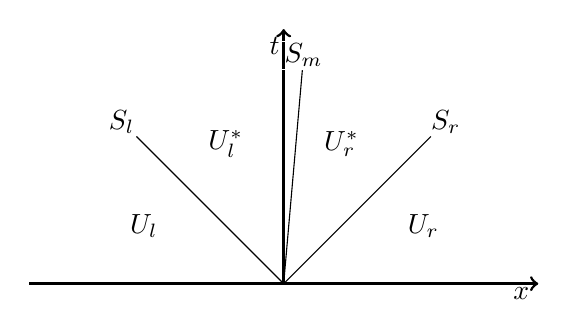
\begin{tikzpicture}[scale = {0.0125\linewidth},inner sep = 1pt]
%% \begin{tikzpicture}[scale = {0.015\linewidth},inner sep = 1pt]
%% \tikzstyle{every node} = [draw,circle,fill=gray!30];
%% \draw (-1.5,0.0) circle (0.8);
%% \draw[<->,line width=1pt] (0,1) node[right]{\;$t$}|-(1,0) node[below]{$m$};
\draw[line width=1pt] (0,0.7) node[left]{$t$}|-(0.7,0) node[below]{$x$};
\draw[->,line width=1pt] (0.7,0)--(0.75,0);
\draw[->,line width=1pt] (0,0.7)--(0,0.75);  
\draw[line width=1pt] (-0,0)--(-0.75,0);
\node[draw=white] (sr) at (0.47730,0.47730) {$S_r$};
\node[draw=white] (cd) at (0.058830,0.67243) {$S_m$};
\node[draw=white] (sl) at (-0.47730,0.47730) {$S_l$};

\node[draw=white] (ur) at (0.41159,0.17049) {$\mbf{U}_{r}$};
\node[draw=white] (usr) at (0.17049,0.41159) {$\mbf{U}^*_{r}$};
\node[draw=white] (usl) at (-0.17049,0.41159) {$\mbf{U}^*_{l}$};
\node[draw=white] (ul) at (-0.41159,0.17049) {$\mbf{U}_{l}$};

\draw (0,0) -- (sr);  
\draw (0,0) -- (cd);  
\draw (0,0) -- (sl);  

\end{tikzpicture}

\end{center}
\caption{Restoration of the contact discontinuity in the HLLC approximate Riemann solver.}
\label{fig:hllc_rstates}
\end{figure}

The approximate solution of the HLLC solver in the $x$-$t$ plane is shown in Figure \ref{fig:hllc_rstates}.  The intermediate states are calculated by approximating the integral over the appropriate Riemann fan and requiring that the Rankine-Hugoniot jump conditions, $v_{nr}^* = v_{nl}^*$, $\mbf{v}_{tr}^* = \mbf{v}_{tl}^*$, and $p_{gr}^* = p_{gl}^*$, are satisfied across the contact discontinuity.  The intermediate states are (Equation (10.33) of \citep{Toro:1999})
\[
\mbf{U}_j^* = 
\rho_j \left( \frac{S_j - v_{nj}}{S_j - v_n^*} \right)
\left[\begin{array}{@{}ccc}
1 \\
v_n \\
\mbf{v}_{t j} \\
\frac{E_j}{\rho_j}  + (S_m - v_{nj}) \left[ S_m + \frac{p_{gj}}{\rho_j(S_j - v_{nj})} \right]  \\
\end{array}\right] \text{ ,} 
\]
where $j=l$ and $j=r$.  The HLLC states are
\begin{gather}
\label{eqn:hllc_states}
\mbf{U}(x,t) = 
\begin{cases}
\mbf{U}_l   & \text{if}\;\;\; 0 < S_l, \\
\mbf{U}_l^*   & \text{if}\;\;\; S_l \le 0 \le S_m, \\
\mbf{U}_r^*   & \text{if}\;\;\; S_m \le 0 \le S_r, \\
\mbf{U}_r   & \text{if}\;\;\; S_r < 0. \\
\end{cases}
\end{gather}
The HLLC fluxes can then be derived with the procedure given in Appendix~\ref{app:hll_flux}.  They are 
\begin{gather}
\label{eqn:hllc_flux}
\mbf{F}(x,t) = 
\begin{cases}
\mbf{F}_l   \phantom{= \mbf{F}_l  + S_l (\mbf{U_l^*} - \mbf{U_l}} & \text{if}\;\;\; 0 < S_l, \\
\mbf{F}_l^* = \mbf{F}_l  + S_l (\mbf{U}_l^* - \mbf{U}_l) & \text{if}\;\;\; S_l \le 0 \le S_m, \\
\mbf{F}_r^* = \mbf{F}_r  + S_r (\mbf{U}_r^* - \mbf{U}_r)  & \text{if}\;\;\; S_m \le 0 \le S_r, \\
\mbf{F}_r  \phantom{= \mbf{F}_r  + S_r (\mbf{U_r^*} - \mbf{U_r}} & \text{if}\;\;\; S_r < 0. \\
\end{cases}
\end{gather}

Both the HLLE and HLLC methods depend on the approximations of the fastest (slowest) wave speed $S_r$ ($S_L$).  \citet{Davis:1988} used wave speeds of 
\begin{gather}
\label{eqn:wave_spd_davis}
S_l = \min \{\lambda_1(\mbf{U}_l),\lambda_1(\mbf{U}_r)\}, \text{ and }
S_r = \max \{\lambda_n(\mbf{U}_l),\lambda_n(\mbf{U}_r)\},
\end{gather} 
where $\lambda_1$ ($\lambda_n$) is the smallest (largest) eigenvalue of \eqref{eqn:nonlinear_sys}.  \citet{Einfeldt:1991} used 
\begin{gather}
\label{eqn:wave_spd_einfeldt}
S_l = \min \{\lambda_1(\mbf{U}_l),\lambda_1(\mbf{U}_{\text{Roe}})\}, \text{ and }
S_r = \max \{\lambda_n(\mbf{U}_r),\lambda_n(\mbf{U}_{\text{Roe}})\},
\end{gather} 
where $\lambda_i(\mbf{U}_{\text{Roe}})$ is an eigenvalue of the Roe matrix, see Section~\ref{sec:roe_solver}.

The middle wave speed, $S_m$, needs to be approximated in the HLLC solver.  \citet{Batten:1997} argued that the middle wave speed should be determined using only  \eqref{eqn:wave_spd_davis} or \eqref{eqn:wave_spd_einfeldt}, and the initial states.  They gave the speed as
\begin{gather}
\label{eqn:wave_spd_batten}
S_m = \frac{(S_r - \vnr)\rho_r \vnr - (S_l - \vnl)\rho_l \vnl - p_{gr} + p_{gl} }
{(S_r - \vnr)\rho_r  - (S_l - \vnl)\rho_l}.
\end{gather}     
\citet{Toro:1994} suggested an alternative method of determining the wave speeds by first estimating the pressure and velocity in the intermediate state according to  
\begin{gather}
\label{eqn:wave_spd_toro}
S_l = \vnl - a_l q_l \text{ , }\;\;\;\; S_m = v_n^* \text{ , }\;\;\;\; S_r = \vnr - a_r q_r \text{ , }
\end{gather}
where
\begin{gather}
\label{eqn:wave_spd_toro2}
q_j = 
\begin{cases}
1 & \text{ if }\;\;\; p_g^* \le p_{gj}, \\ 
\left[ 1 + \frac{\gamma + 1}{2\gamma} \left( \frac{p^*_g}{p_{gj}} - 1 \right) \right]^{\frac{1}{2}} & 
\text{ if }\;\;\; p_g^* > p_{gj},
\end{cases}
\end{gather}
for $j=l$ and $j=r$.

%-----------------------------------------------------------------
% Isolated CD HLLE, HLLC, Roe
%-----------------------------------------------------------------
\begin{figure}[htbp]
\begin{tabular}{cc}
\resizebox{0.5\linewidth}{!}{\tikzsetnextfilename{toro7_hlle_1}\begin{tikzpicture}[gnuplot]
%% generated with GNUPLOT 4.6p4 (Lua 5.1; terminal rev. 99, script rev. 100)
%% Tue 01 Jul 2014 10:59:57 AM EDT
\path (0.000,0.000) rectangle (8.000,6.000);
\gpfill{rgb color={1.000,1.000,1.000}} (1.012,0.985)--(7.446,0.985)--(7.446,5.630)--(1.012,5.630)--cycle;
\gpcolor{color=gp lt color border}
\gpsetlinetype{gp lt border}
\gpsetlinewidth{1.00}
\draw[gp path] (1.012,0.985)--(1.012,5.630)--(7.446,5.630)--(7.446,0.985)--cycle;
\gpcolor{color=gp lt color axes}
\gpsetlinetype{gp lt axes}
\gpsetlinewidth{2.00}
\draw[gp path] (1.012,0.985)--(7.447,0.985);
\gpcolor{color=gp lt color border}
\gpsetlinetype{gp lt border}
\draw[gp path] (1.012,0.985)--(1.084,0.985);
\draw[gp path] (7.447,0.985)--(7.375,0.985);
\gpcolor{rgb color={0.000,0.000,0.000}}
\node[gp node right,font={\fontsize{10pt}{12pt}\selectfont}] at (0.828,0.985) {0.9};
\gpcolor{color=gp lt color axes}
\gpsetlinetype{gp lt axes}
\draw[gp path] (1.012,1.759)--(7.447,1.759);
\gpcolor{color=gp lt color border}
\gpsetlinetype{gp lt border}
\draw[gp path] (1.012,1.759)--(1.084,1.759);
\draw[gp path] (7.447,1.759)--(7.375,1.759);
\gpcolor{rgb color={0.000,0.000,0.000}}
\node[gp node right,font={\fontsize{10pt}{12pt}\selectfont}] at (0.828,1.759) {1};
\gpcolor{color=gp lt color axes}
\gpsetlinetype{gp lt axes}
\draw[gp path] (1.012,2.534)--(7.447,2.534);
\gpcolor{color=gp lt color border}
\gpsetlinetype{gp lt border}
\draw[gp path] (1.012,2.534)--(1.084,2.534);
\draw[gp path] (7.447,2.534)--(7.375,2.534);
\gpcolor{rgb color={0.000,0.000,0.000}}
\node[gp node right,font={\fontsize{10pt}{12pt}\selectfont}] at (0.828,2.534) {1.1};
\gpcolor{color=gp lt color axes}
\gpsetlinetype{gp lt axes}
\draw[gp path] (1.012,3.308)--(7.447,3.308);
\gpcolor{color=gp lt color border}
\gpsetlinetype{gp lt border}
\draw[gp path] (1.012,3.308)--(1.084,3.308);
\draw[gp path] (7.447,3.308)--(7.375,3.308);
\gpcolor{rgb color={0.000,0.000,0.000}}
\node[gp node right,font={\fontsize{10pt}{12pt}\selectfont}] at (0.828,3.308) {1.2};
\gpcolor{color=gp lt color axes}
\gpsetlinetype{gp lt axes}
\draw[gp path] (1.012,4.082)--(7.447,4.082);
\gpcolor{color=gp lt color border}
\gpsetlinetype{gp lt border}
\draw[gp path] (1.012,4.082)--(1.084,4.082);
\draw[gp path] (7.447,4.082)--(7.375,4.082);
\gpcolor{rgb color={0.000,0.000,0.000}}
\node[gp node right,font={\fontsize{10pt}{12pt}\selectfont}] at (0.828,4.082) {1.3};
\gpcolor{color=gp lt color axes}
\gpsetlinetype{gp lt axes}
\draw[gp path] (1.012,4.857)--(7.447,4.857);
\gpcolor{color=gp lt color border}
\gpsetlinetype{gp lt border}
\draw[gp path] (1.012,4.857)--(1.084,4.857);
\draw[gp path] (7.447,4.857)--(7.375,4.857);
\gpcolor{rgb color={0.000,0.000,0.000}}
\node[gp node right,font={\fontsize{10pt}{12pt}\selectfont}] at (0.828,4.857) {1.4};
\gpcolor{color=gp lt color axes}
\gpsetlinetype{gp lt axes}
\draw[gp path] (1.012,5.631)--(7.447,5.631);
\gpcolor{color=gp lt color border}
\gpsetlinetype{gp lt border}
\draw[gp path] (1.012,5.631)--(1.084,5.631);
\draw[gp path] (7.447,5.631)--(7.375,5.631);
\gpcolor{rgb color={0.000,0.000,0.000}}
\node[gp node right,font={\fontsize{10pt}{12pt}\selectfont}] at (0.828,5.631) {1.5};
\gpcolor{color=gp lt color axes}
\gpsetlinetype{gp lt axes}
\draw[gp path] (1.012,0.985)--(1.012,5.631);
\gpcolor{color=gp lt color border}
\gpsetlinetype{gp lt border}
\draw[gp path] (1.012,0.985)--(1.012,1.057);
\draw[gp path] (1.012,5.631)--(1.012,5.559);
\gpcolor{rgb color={0.000,0.000,0.000}}
\node[gp node center,font={\fontsize{10pt}{12pt}\selectfont}] at (1.012,0.677) {0};
\gpcolor{color=gp lt color axes}
\gpsetlinetype{gp lt axes}
\draw[gp path] (2.299,0.985)--(2.299,5.631);
\gpcolor{color=gp lt color border}
\gpsetlinetype{gp lt border}
\draw[gp path] (2.299,0.985)--(2.299,1.057);
\draw[gp path] (2.299,5.631)--(2.299,5.559);
\gpcolor{rgb color={0.000,0.000,0.000}}
\node[gp node center,font={\fontsize{10pt}{12pt}\selectfont}] at (2.299,0.677) {0.2};
\gpcolor{color=gp lt color axes}
\gpsetlinetype{gp lt axes}
\draw[gp path] (3.586,0.985)--(3.586,5.631);
\gpcolor{color=gp lt color border}
\gpsetlinetype{gp lt border}
\draw[gp path] (3.586,0.985)--(3.586,1.057);
\draw[gp path] (3.586,5.631)--(3.586,5.559);
\gpcolor{rgb color={0.000,0.000,0.000}}
\node[gp node center,font={\fontsize{10pt}{12pt}\selectfont}] at (3.586,0.677) {0.4};
\gpcolor{color=gp lt color axes}
\gpsetlinetype{gp lt axes}
\draw[gp path] (4.873,0.985)--(4.873,5.631);
\gpcolor{color=gp lt color border}
\gpsetlinetype{gp lt border}
\draw[gp path] (4.873,0.985)--(4.873,1.057);
\draw[gp path] (4.873,5.631)--(4.873,5.559);
\gpcolor{rgb color={0.000,0.000,0.000}}
\node[gp node center,font={\fontsize{10pt}{12pt}\selectfont}] at (4.873,0.677) {0.6};
\gpcolor{color=gp lt color axes}
\gpsetlinetype{gp lt axes}
\draw[gp path] (6.160,0.985)--(6.160,5.631);
\gpcolor{color=gp lt color border}
\gpsetlinetype{gp lt border}
\draw[gp path] (6.160,0.985)--(6.160,1.057);
\draw[gp path] (6.160,5.631)--(6.160,5.559);
\gpcolor{rgb color={0.000,0.000,0.000}}
\node[gp node center,font={\fontsize{10pt}{12pt}\selectfont}] at (6.160,0.677) {0.8};
\gpcolor{color=gp lt color axes}
\gpsetlinetype{gp lt axes}
\draw[gp path] (7.447,0.985)--(7.447,5.631);
\gpcolor{color=gp lt color border}
\gpsetlinetype{gp lt border}
\draw[gp path] (7.447,0.985)--(7.447,1.057);
\draw[gp path] (7.447,5.631)--(7.447,5.559);
\gpcolor{rgb color={0.000,0.000,0.000}}
\node[gp node center,font={\fontsize{10pt}{12pt}\selectfont}] at (7.447,0.677) {1};
\gpcolor{color=gp lt color border}
\draw[gp path] (1.012,5.631)--(1.012,0.985)--(7.447,0.985)--(7.447,5.631)--cycle;
\gpcolor{rgb color={0.000,0.000,0.000}}
\node[gp node center,font={\fontsize{10pt}{12pt}\selectfont}] at (4.229,0.215) {\huge $x$};
\gpcolor{rgb color={1.000,0.000,0.000}}
\gpsetlinewidth{0.50}
\gpsetpointsize{4.44}
\gppoint{gp mark 7}{(1.037,4.857)}
\gppoint{gp mark 7}{(1.087,4.857)}
\gppoint{gp mark 7}{(1.138,4.857)}
\gppoint{gp mark 7}{(1.188,4.857)}
\gppoint{gp mark 7}{(1.238,4.857)}
\gppoint{gp mark 7}{(1.289,4.857)}
\gppoint{gp mark 7}{(1.339,4.857)}
\gppoint{gp mark 7}{(1.389,4.857)}
\gppoint{gp mark 7}{(1.439,4.857)}
\gppoint{gp mark 7}{(1.490,4.857)}
\gppoint{gp mark 7}{(1.540,4.857)}
\gppoint{gp mark 7}{(1.590,4.857)}
\gppoint{gp mark 7}{(1.640,4.857)}
\gppoint{gp mark 7}{(1.691,4.857)}
\gppoint{gp mark 7}{(1.741,4.857)}
\gppoint{gp mark 7}{(1.791,4.857)}
\gppoint{gp mark 7}{(1.842,4.857)}
\gppoint{gp mark 7}{(1.892,4.857)}
\gppoint{gp mark 7}{(1.942,4.857)}
\gppoint{gp mark 7}{(1.992,4.857)}
\gppoint{gp mark 7}{(2.043,4.857)}
\gppoint{gp mark 7}{(2.093,4.857)}
\gppoint{gp mark 7}{(2.143,4.857)}
\gppoint{gp mark 7}{(2.193,4.857)}
\gppoint{gp mark 7}{(2.244,4.857)}
\gppoint{gp mark 7}{(2.294,4.857)}
\gppoint{gp mark 7}{(2.344,4.857)}
\gppoint{gp mark 7}{(2.395,4.856)}
\gppoint{gp mark 7}{(2.445,4.856)}
\gppoint{gp mark 7}{(2.495,4.856)}
\gppoint{gp mark 7}{(2.545,4.856)}
\gppoint{gp mark 7}{(2.596,4.856)}
\gppoint{gp mark 7}{(2.646,4.856)}
\gppoint{gp mark 7}{(2.696,4.856)}
\gppoint{gp mark 7}{(2.746,4.856)}
\gppoint{gp mark 7}{(2.797,4.855)}
\gppoint{gp mark 7}{(2.847,4.855)}
\gppoint{gp mark 7}{(2.897,4.855)}
\gppoint{gp mark 7}{(2.948,4.854)}
\gppoint{gp mark 7}{(2.998,4.854)}
\gppoint{gp mark 7}{(3.048,4.853)}
\gppoint{gp mark 7}{(3.098,4.852)}
\gppoint{gp mark 7}{(3.149,4.851)}
\gppoint{gp mark 7}{(3.199,4.850)}
\gppoint{gp mark 7}{(3.249,4.849)}
\gppoint{gp mark 7}{(3.299,4.847)}
\gppoint{gp mark 7}{(3.350,4.845)}
\gppoint{gp mark 7}{(3.400,4.843)}
\gppoint{gp mark 7}{(3.450,4.840)}
\gppoint{gp mark 7}{(3.501,4.836)}
\gppoint{gp mark 7}{(3.551,4.833)}
\gppoint{gp mark 7}{(3.601,4.828)}
\gppoint{gp mark 7}{(3.651,4.823)}
\gppoint{gp mark 7}{(3.702,4.817)}
\gppoint{gp mark 7}{(3.752,4.810)}
\gppoint{gp mark 7}{(3.802,4.802)}
\gppoint{gp mark 7}{(3.852,4.793)}
\gppoint{gp mark 7}{(3.903,4.782)}
\gppoint{gp mark 7}{(3.953,4.770)}
\gppoint{gp mark 7}{(4.003,4.757)}
\gppoint{gp mark 7}{(4.054,4.742)}
\gppoint{gp mark 7}{(4.104,4.725)}
\gppoint{gp mark 7}{(4.154,4.707)}
\gppoint{gp mark 7}{(4.204,4.686)}
\gppoint{gp mark 7}{(4.255,4.663)}
\gppoint{gp mark 7}{(4.305,4.638)}
\gppoint{gp mark 7}{(4.355,4.610)}
\gppoint{gp mark 7}{(4.405,4.580)}
\gppoint{gp mark 7}{(4.456,4.547)}
\gppoint{gp mark 7}{(4.506,4.512)}
\gppoint{gp mark 7}{(4.556,4.474)}
\gppoint{gp mark 7}{(4.607,4.432)}
\gppoint{gp mark 7}{(4.657,4.388)}
\gppoint{gp mark 7}{(4.707,4.342)}
\gppoint{gp mark 7}{(4.757,4.292)}
\gppoint{gp mark 7}{(4.808,4.239)}
\gppoint{gp mark 7}{(4.858,4.184)}
\gppoint{gp mark 7}{(4.908,4.126)}
\gppoint{gp mark 7}{(4.958,4.066)}
\gppoint{gp mark 7}{(5.009,4.003)}
\gppoint{gp mark 7}{(5.059,3.938)}
\gppoint{gp mark 7}{(5.109,3.871)}
\gppoint{gp mark 7}{(5.160,3.802)}
\gppoint{gp mark 7}{(5.210,3.732)}
\gppoint{gp mark 7}{(5.260,3.660)}
\gppoint{gp mark 7}{(5.310,3.587)}
\gppoint{gp mark 7}{(5.361,3.514)}
\gppoint{gp mark 7}{(5.411,3.439)}
\gppoint{gp mark 7}{(5.461,3.365)}
\gppoint{gp mark 7}{(5.511,3.291)}
\gppoint{gp mark 7}{(5.562,3.217)}
\gppoint{gp mark 7}{(5.612,3.143)}
\gppoint{gp mark 7}{(5.662,3.070)}
\gppoint{gp mark 7}{(5.713,2.999)}
\gppoint{gp mark 7}{(5.763,2.928)}
\gppoint{gp mark 7}{(5.813,2.859)}
\gppoint{gp mark 7}{(5.863,2.792)}
\gppoint{gp mark 7}{(5.914,2.727)}
\gppoint{gp mark 7}{(5.964,2.663)}
\gppoint{gp mark 7}{(6.014,2.602)}
\gppoint{gp mark 7}{(6.064,2.543)}
\gppoint{gp mark 7}{(6.115,2.487)}
\gppoint{gp mark 7}{(6.165,2.432)}
\gppoint{gp mark 7}{(6.215,2.381)}
\gppoint{gp mark 7}{(6.266,2.332)}
\gppoint{gp mark 7}{(6.316,2.285)}
\gppoint{gp mark 7}{(6.366,2.242)}
\gppoint{gp mark 7}{(6.416,2.200)}
\gppoint{gp mark 7}{(6.467,2.161)}
\gppoint{gp mark 7}{(6.517,2.125)}
\gppoint{gp mark 7}{(6.567,2.091)}
\gppoint{gp mark 7}{(6.617,2.060)}
\gppoint{gp mark 7}{(6.668,2.031)}
\gppoint{gp mark 7}{(6.718,2.004)}
\gppoint{gp mark 7}{(6.768,1.979)}
\gppoint{gp mark 7}{(6.819,1.956)}
\gppoint{gp mark 7}{(6.869,1.935)}
\gppoint{gp mark 7}{(6.919,1.916)}
\gppoint{gp mark 7}{(6.969,1.899)}
\gppoint{gp mark 7}{(7.020,1.883)}
\gppoint{gp mark 7}{(7.070,1.870)}
\gppoint{gp mark 7}{(7.120,1.857)}
\gppoint{gp mark 7}{(7.170,1.847)}
\gppoint{gp mark 7}{(7.221,1.837)}
\gppoint{gp mark 7}{(7.271,1.830)}
\gppoint{gp mark 7}{(7.321,1.824)}
\gppoint{gp mark 7}{(7.372,1.819)}
\gppoint{gp mark 7}{(7.422,1.817)}
\gpcolor{rgb color={0.000,0.000,0.000}}
\gpsetlinetype{gp lt plot 0}
\gpsetlinewidth{4.00}
\draw[gp path] (1.018,4.857)--(1.031,4.857)--(1.043,4.857)--(1.056,4.857)--(1.069,4.857)%
  --(1.081,4.857)--(1.094,4.857)--(1.106,4.857)--(1.119,4.857)--(1.131,4.857)--(1.144,4.857)%
  --(1.157,4.857)--(1.169,4.857)--(1.182,4.857)--(1.194,4.857)--(1.207,4.857)--(1.219,4.857)%
  --(1.232,4.857)--(1.245,4.857)--(1.257,4.857)--(1.270,4.857)--(1.282,4.857)--(1.295,4.857)%
  --(1.307,4.857)--(1.320,4.857)--(1.332,4.857)--(1.345,4.857)--(1.358,4.857)--(1.370,4.857)%
  --(1.383,4.857)--(1.395,4.857)--(1.408,4.857)--(1.420,4.857)--(1.433,4.857)--(1.446,4.857)%
  --(1.458,4.857)--(1.471,4.857)--(1.483,4.857)--(1.496,4.857)--(1.508,4.857)--(1.521,4.857)%
  --(1.534,4.857)--(1.546,4.857)--(1.559,4.857)--(1.571,4.857)--(1.584,4.857)--(1.596,4.857)%
  --(1.609,4.857)--(1.622,4.857)--(1.634,4.857)--(1.647,4.857)--(1.659,4.857)--(1.672,4.857)%
  --(1.684,4.857)--(1.697,4.857)--(1.710,4.857)--(1.722,4.857)--(1.735,4.857)--(1.747,4.857)%
  --(1.760,4.857)--(1.772,4.857)--(1.785,4.857)--(1.798,4.857)--(1.810,4.857)--(1.823,4.857)%
  --(1.835,4.857)--(1.848,4.857)--(1.860,4.857)--(1.873,4.857)--(1.886,4.857)--(1.898,4.857)%
  --(1.911,4.857)--(1.923,4.857)--(1.936,4.857)--(1.948,4.857)--(1.961,4.857)--(1.973,4.857)%
  --(1.986,4.857)--(1.999,4.857)--(2.011,4.857)--(2.024,4.857)--(2.036,4.857)--(2.049,4.857)%
  --(2.061,4.857)--(2.074,4.857)--(2.087,4.857)--(2.099,4.857)--(2.112,4.857)--(2.124,4.857)%
  --(2.137,4.857)--(2.149,4.857)--(2.162,4.857)--(2.175,4.857)--(2.187,4.857)--(2.200,4.857)%
  --(2.212,4.857)--(2.225,4.857)--(2.237,4.857)--(2.250,4.857)--(2.263,4.857)--(2.275,4.857)%
  --(2.288,4.857)--(2.300,4.857)--(2.313,4.857)--(2.325,4.857)--(2.338,4.857)--(2.351,4.857)%
  --(2.363,4.857)--(2.376,4.857)--(2.388,4.857)--(2.401,4.857)--(2.413,4.857)--(2.426,4.857)%
  --(2.439,4.857)--(2.451,4.857)--(2.464,4.857)--(2.476,4.857)--(2.489,4.857)--(2.501,4.857)%
  --(2.514,4.857)--(2.526,4.857)--(2.539,4.857)--(2.552,4.857)--(2.564,4.857)--(2.577,4.857)%
  --(2.589,4.857)--(2.602,4.857)--(2.614,4.857)--(2.627,4.857)--(2.640,4.857)--(2.652,4.857)%
  --(2.665,4.857)--(2.677,4.857)--(2.690,4.857)--(2.702,4.857)--(2.715,4.857)--(2.728,4.857)%
  --(2.740,4.857)--(2.753,4.857)--(2.765,4.857)--(2.778,4.857)--(2.790,4.857)--(2.803,4.857)%
  --(2.816,4.857)--(2.828,4.857)--(2.841,4.857)--(2.853,4.857)--(2.866,4.857)--(2.878,4.857)%
  --(2.891,4.857)--(2.904,4.857)--(2.916,4.857)--(2.929,4.857)--(2.941,4.857)--(2.954,4.857)%
  --(2.966,4.857)--(2.979,4.857)--(2.992,4.857)--(3.004,4.857)--(3.017,4.857)--(3.029,4.857)%
  --(3.042,4.857)--(3.054,4.857)--(3.067,4.857)--(3.079,4.857)--(3.092,4.857)--(3.105,4.857)%
  --(3.117,4.857)--(3.130,4.857)--(3.142,4.857)--(3.155,4.857)--(3.167,4.857)--(3.180,4.857)%
  --(3.193,4.857)--(3.205,4.857)--(3.218,4.857)--(3.230,4.857)--(3.243,4.857)--(3.255,4.857)%
  --(3.268,4.857)--(3.281,4.857)--(3.293,4.857)--(3.306,4.857)--(3.318,4.857)--(3.331,4.857)%
  --(3.343,4.857)--(3.356,4.857)--(3.369,4.857)--(3.381,4.857)--(3.394,4.857)--(3.406,4.857)%
  --(3.419,4.857)--(3.431,4.857)--(3.444,4.857)--(3.457,4.857)--(3.469,4.857)--(3.482,4.857)%
  --(3.494,4.857)--(3.507,4.857)--(3.519,4.857)--(3.532,4.857)--(3.545,4.857)--(3.557,4.857)%
  --(3.570,4.857)--(3.582,4.857)--(3.595,4.857)--(3.607,4.857)--(3.620,4.857)--(3.633,4.857)%
  --(3.645,4.857)--(3.658,4.857)--(3.670,4.857)--(3.683,4.857)--(3.695,4.857)--(3.708,4.857)%
  --(3.720,4.857)--(3.733,4.857)--(3.746,4.857)--(3.758,4.857)--(3.771,4.857)--(3.783,4.857)%
  --(3.796,4.857)--(3.808,4.857)--(3.821,4.857)--(3.834,4.857)--(3.846,4.857)--(3.859,4.857)%
  --(3.871,4.857)--(3.884,4.857)--(3.896,4.857)--(3.909,4.857)--(3.922,4.857)--(3.934,4.857)%
  --(3.947,4.857)--(3.959,4.857)--(3.972,4.857)--(3.984,4.857)--(3.997,4.857)--(4.010,4.857)%
  --(4.022,4.857)--(4.035,4.857)--(4.047,4.857)--(4.060,4.857)--(4.072,4.857)--(4.085,4.857)%
  --(4.098,4.857)--(4.110,4.857)--(4.123,4.857)--(4.135,4.857)--(4.148,4.857)--(4.160,4.857)%
  --(4.173,4.857)--(4.186,4.857)--(4.198,4.857)--(4.211,4.857)--(4.223,4.857)--(4.236,4.857)%
  --(4.248,4.857)--(4.261,4.857)--(4.273,4.857)--(4.286,4.857)--(4.299,4.857)--(4.311,4.857)%
  --(4.324,4.857)--(4.336,4.857)--(4.349,4.857)--(4.361,4.857)--(4.374,4.857)--(4.387,4.857)%
  --(4.399,4.857)--(4.412,4.857)--(4.424,4.857)--(4.437,4.857)--(4.449,4.857)--(4.462,4.857)%
  --(4.475,4.857)--(4.487,4.857)--(4.500,4.857)--(4.512,4.857)--(4.525,4.857)--(4.537,4.857)%
  --(4.550,4.857)--(4.563,4.857)--(4.575,4.857)--(4.588,4.857)--(4.600,4.857)--(4.613,4.857)%
  --(4.625,4.857)--(4.638,4.857)--(4.651,4.857)--(4.663,4.857)--(4.676,4.857)--(4.688,4.857)%
  --(4.701,4.857)--(4.713,4.857)--(4.726,4.857)--(4.739,4.857)--(4.751,4.857)--(4.764,4.857)%
  --(4.776,4.857)--(4.789,4.857)--(4.801,4.857)--(4.814,4.857)--(4.826,4.857)--(4.839,4.857)%
  --(4.852,4.857)--(4.864,4.857)--(4.877,4.857)--(4.889,4.857)--(4.902,4.857)--(4.914,4.857)%
  --(4.927,4.857)--(4.940,4.857)--(4.952,4.857)--(4.965,4.857)--(4.977,4.857)--(4.990,4.857)%
  --(5.002,4.857)--(5.015,4.857)--(5.028,4.857)--(5.040,4.857)--(5.053,4.857)--(5.065,4.857)%
  --(5.078,4.857)--(5.090,4.857)--(5.103,4.857)--(5.116,4.857)--(5.128,4.857)--(5.141,4.857)%
  --(5.153,4.857)--(5.166,4.857)--(5.178,4.857)--(5.191,4.857)--(5.204,4.857)--(5.216,4.857)%
  --(5.229,4.857)--(5.241,4.857)--(5.254,4.857)--(5.266,4.857)--(5.279,4.857)--(5.292,4.857)%
  --(5.304,4.857)--(5.317,4.857)--(5.329,4.857)--(5.342,4.857)--(5.354,4.857)--(5.367,4.857)%
  --(5.380,4.857)--(5.392,4.857)--(5.405,4.857)--(5.417,4.857)--(5.430,4.857)--(5.442,4.857)%
  --(5.455,4.857)--(5.467,4.857)--(5.480,4.857)--(5.493,4.857)--(5.505,4.857)--(5.518,1.759)%
  --(5.530,1.759)--(5.543,1.759)--(5.555,1.759)--(5.568,1.759)--(5.581,1.759)--(5.593,1.759)%
  --(5.606,1.759)--(5.618,1.759)--(5.631,1.759)--(5.643,1.759)--(5.656,1.759)--(5.669,1.759)%
  --(5.681,1.759)--(5.694,1.759)--(5.706,1.759)--(5.719,1.759)--(5.731,1.759)--(5.744,1.759)%
  --(5.757,1.759)--(5.769,1.759)--(5.782,1.759)--(5.794,1.759)--(5.807,1.759)--(5.819,1.759)%
  --(5.832,1.759)--(5.845,1.759)--(5.857,1.759)--(5.870,1.759)--(5.882,1.759)--(5.895,1.759)%
  --(5.907,1.759)--(5.920,1.759)--(5.933,1.759)--(5.945,1.759)--(5.958,1.759)--(5.970,1.759)%
  --(5.983,1.759)--(5.995,1.759)--(6.008,1.759)--(6.020,1.759)--(6.033,1.759)--(6.046,1.759)%
  --(6.058,1.759)--(6.071,1.759)--(6.083,1.759)--(6.096,1.759)--(6.108,1.759)--(6.121,1.759)%
  --(6.134,1.759)--(6.146,1.759)--(6.159,1.759)--(6.171,1.759)--(6.184,1.759)--(6.196,1.759)%
  --(6.209,1.759)--(6.222,1.759)--(6.234,1.759)--(6.247,1.759)--(6.259,1.759)--(6.272,1.759)%
  --(6.284,1.759)--(6.297,1.759)--(6.310,1.759)--(6.322,1.759)--(6.335,1.759)--(6.347,1.759)%
  --(6.360,1.759)--(6.372,1.759)--(6.385,1.759)--(6.398,1.759)--(6.410,1.759)--(6.423,1.759)%
  --(6.435,1.759)--(6.448,1.759)--(6.460,1.759)--(6.473,1.759)--(6.486,1.759)--(6.498,1.759)%
  --(6.511,1.759)--(6.523,1.759)--(6.536,1.759)--(6.548,1.759)--(6.561,1.759)--(6.573,1.759)%
  --(6.586,1.759)--(6.599,1.759)--(6.611,1.759)--(6.624,1.759)--(6.636,1.759)--(6.649,1.759)%
  --(6.661,1.759)--(6.674,1.759)--(6.687,1.759)--(6.699,1.759)--(6.712,1.759)--(6.724,1.759)%
  --(6.737,1.759)--(6.749,1.759)--(6.762,1.759)--(6.775,1.759)--(6.787,1.759)--(6.800,1.759)%
  --(6.812,1.759)--(6.825,1.759)--(6.837,1.759)--(6.850,1.759)--(6.863,1.759)--(6.875,1.759)%
  --(6.888,1.759)--(6.900,1.759)--(6.913,1.759)--(6.925,1.759)--(6.938,1.759)--(6.951,1.759)%
  --(6.963,1.759)--(6.976,1.759)--(6.988,1.759)--(7.001,1.759)--(7.013,1.759)--(7.026,1.759)%
  --(7.039,1.759)--(7.051,1.759)--(7.064,1.759)--(7.076,1.759)--(7.089,1.759)--(7.101,1.759)%
  --(7.114,1.759)--(7.127,1.759)--(7.139,1.759)--(7.152,1.759)--(7.164,1.759)--(7.177,1.759)%
  --(7.189,1.759)--(7.202,1.759)--(7.214,1.759)--(7.227,1.759)--(7.240,1.759)--(7.252,1.759)%
  --(7.265,1.759)--(7.277,1.759)--(7.290,1.759)--(7.302,1.759)--(7.315,1.759)--(7.328,1.759)%
  --(7.340,1.759)--(7.353,1.759)--(7.365,1.759)--(7.378,1.759)--(7.390,1.759)--(7.403,1.759)%
  --(7.416,1.759)--(7.428,1.759)--(7.441,1.759);
\node[gp node left,font={\fontsize{10pt}{12pt}\selectfont}] at (1.334,4.470) {\huge $\rho$};
\node[gp node left,font={\fontsize{10pt}{12pt}\selectfont}] at (1.173,1.953) {\huge HLLE};
%% coordinates of the plot area
\gpdefrectangularnode{gp plot 1}{\pgfpoint{1.012cm}{0.985cm}}{\pgfpoint{7.447cm}{5.631cm}}
\end{tikzpicture}
%% gnuplot variables
} &
\resizebox{0.5\linewidth}{!}{\tikzsetnextfilename{toro7_hllc_1}\begin{tikzpicture}[gnuplot]
%% generated with GNUPLOT 4.6p4 (Lua 5.1; terminal rev. 99, script rev. 100)
%% Tue 01 Jul 2014 11:00:07 AM EDT
\path (0.000,0.000) rectangle (8.000,6.000);
\gpfill{rgb color={1.000,1.000,1.000}} (1.012,0.985)--(7.446,0.985)--(7.446,5.630)--(1.012,5.630)--cycle;
\gpcolor{color=gp lt color border}
\gpsetlinetype{gp lt border}
\gpsetlinewidth{1.00}
\draw[gp path] (1.012,0.985)--(1.012,5.630)--(7.446,5.630)--(7.446,0.985)--cycle;
\gpcolor{color=gp lt color axes}
\gpsetlinetype{gp lt axes}
\gpsetlinewidth{2.00}
\draw[gp path] (1.012,0.985)--(7.447,0.985);
\gpcolor{color=gp lt color border}
\gpsetlinetype{gp lt border}
\draw[gp path] (1.012,0.985)--(1.084,0.985);
\draw[gp path] (7.447,0.985)--(7.375,0.985);
\gpcolor{rgb color={0.000,0.000,0.000}}
\node[gp node right,font={\fontsize{10pt}{12pt}\selectfont}] at (0.828,0.985) {0.9};
\gpcolor{color=gp lt color axes}
\gpsetlinetype{gp lt axes}
\draw[gp path] (1.012,1.759)--(7.447,1.759);
\gpcolor{color=gp lt color border}
\gpsetlinetype{gp lt border}
\draw[gp path] (1.012,1.759)--(1.084,1.759);
\draw[gp path] (7.447,1.759)--(7.375,1.759);
\gpcolor{rgb color={0.000,0.000,0.000}}
\node[gp node right,font={\fontsize{10pt}{12pt}\selectfont}] at (0.828,1.759) {1};
\gpcolor{color=gp lt color axes}
\gpsetlinetype{gp lt axes}
\draw[gp path] (1.012,2.534)--(7.447,2.534);
\gpcolor{color=gp lt color border}
\gpsetlinetype{gp lt border}
\draw[gp path] (1.012,2.534)--(1.084,2.534);
\draw[gp path] (7.447,2.534)--(7.375,2.534);
\gpcolor{rgb color={0.000,0.000,0.000}}
\node[gp node right,font={\fontsize{10pt}{12pt}\selectfont}] at (0.828,2.534) {1.1};
\gpcolor{color=gp lt color axes}
\gpsetlinetype{gp lt axes}
\draw[gp path] (1.012,3.308)--(7.447,3.308);
\gpcolor{color=gp lt color border}
\gpsetlinetype{gp lt border}
\draw[gp path] (1.012,3.308)--(1.084,3.308);
\draw[gp path] (7.447,3.308)--(7.375,3.308);
\gpcolor{rgb color={0.000,0.000,0.000}}
\node[gp node right,font={\fontsize{10pt}{12pt}\selectfont}] at (0.828,3.308) {1.2};
\gpcolor{color=gp lt color axes}
\gpsetlinetype{gp lt axes}
\draw[gp path] (1.012,4.082)--(7.447,4.082);
\gpcolor{color=gp lt color border}
\gpsetlinetype{gp lt border}
\draw[gp path] (1.012,4.082)--(1.084,4.082);
\draw[gp path] (7.447,4.082)--(7.375,4.082);
\gpcolor{rgb color={0.000,0.000,0.000}}
\node[gp node right,font={\fontsize{10pt}{12pt}\selectfont}] at (0.828,4.082) {1.3};
\gpcolor{color=gp lt color axes}
\gpsetlinetype{gp lt axes}
\draw[gp path] (1.012,4.857)--(7.447,4.857);
\gpcolor{color=gp lt color border}
\gpsetlinetype{gp lt border}
\draw[gp path] (1.012,4.857)--(1.084,4.857);
\draw[gp path] (7.447,4.857)--(7.375,4.857);
\gpcolor{rgb color={0.000,0.000,0.000}}
\node[gp node right,font={\fontsize{10pt}{12pt}\selectfont}] at (0.828,4.857) {1.4};
\gpcolor{color=gp lt color axes}
\gpsetlinetype{gp lt axes}
\draw[gp path] (1.012,5.631)--(7.447,5.631);
\gpcolor{color=gp lt color border}
\gpsetlinetype{gp lt border}
\draw[gp path] (1.012,5.631)--(1.084,5.631);
\draw[gp path] (7.447,5.631)--(7.375,5.631);
\gpcolor{rgb color={0.000,0.000,0.000}}
\node[gp node right,font={\fontsize{10pt}{12pt}\selectfont}] at (0.828,5.631) {1.5};
\gpcolor{color=gp lt color axes}
\gpsetlinetype{gp lt axes}
\draw[gp path] (1.012,0.985)--(1.012,5.631);
\gpcolor{color=gp lt color border}
\gpsetlinetype{gp lt border}
\draw[gp path] (1.012,0.985)--(1.012,1.057);
\draw[gp path] (1.012,5.631)--(1.012,5.559);
\gpcolor{rgb color={0.000,0.000,0.000}}
\node[gp node center,font={\fontsize{10pt}{12pt}\selectfont}] at (1.012,0.677) {0};
\gpcolor{color=gp lt color axes}
\gpsetlinetype{gp lt axes}
\draw[gp path] (2.299,0.985)--(2.299,5.631);
\gpcolor{color=gp lt color border}
\gpsetlinetype{gp lt border}
\draw[gp path] (2.299,0.985)--(2.299,1.057);
\draw[gp path] (2.299,5.631)--(2.299,5.559);
\gpcolor{rgb color={0.000,0.000,0.000}}
\node[gp node center,font={\fontsize{10pt}{12pt}\selectfont}] at (2.299,0.677) {0.2};
\gpcolor{color=gp lt color axes}
\gpsetlinetype{gp lt axes}
\draw[gp path] (3.586,0.985)--(3.586,5.631);
\gpcolor{color=gp lt color border}
\gpsetlinetype{gp lt border}
\draw[gp path] (3.586,0.985)--(3.586,1.057);
\draw[gp path] (3.586,5.631)--(3.586,5.559);
\gpcolor{rgb color={0.000,0.000,0.000}}
\node[gp node center,font={\fontsize{10pt}{12pt}\selectfont}] at (3.586,0.677) {0.4};
\gpcolor{color=gp lt color axes}
\gpsetlinetype{gp lt axes}
\draw[gp path] (4.873,0.985)--(4.873,5.631);
\gpcolor{color=gp lt color border}
\gpsetlinetype{gp lt border}
\draw[gp path] (4.873,0.985)--(4.873,1.057);
\draw[gp path] (4.873,5.631)--(4.873,5.559);
\gpcolor{rgb color={0.000,0.000,0.000}}
\node[gp node center,font={\fontsize{10pt}{12pt}\selectfont}] at (4.873,0.677) {0.6};
\gpcolor{color=gp lt color axes}
\gpsetlinetype{gp lt axes}
\draw[gp path] (6.160,0.985)--(6.160,5.631);
\gpcolor{color=gp lt color border}
\gpsetlinetype{gp lt border}
\draw[gp path] (6.160,0.985)--(6.160,1.057);
\draw[gp path] (6.160,5.631)--(6.160,5.559);
\gpcolor{rgb color={0.000,0.000,0.000}}
\node[gp node center,font={\fontsize{10pt}{12pt}\selectfont}] at (6.160,0.677) {0.8};
\gpcolor{color=gp lt color axes}
\gpsetlinetype{gp lt axes}
\draw[gp path] (7.447,0.985)--(7.447,5.631);
\gpcolor{color=gp lt color border}
\gpsetlinetype{gp lt border}
\draw[gp path] (7.447,0.985)--(7.447,1.057);
\draw[gp path] (7.447,5.631)--(7.447,5.559);
\gpcolor{rgb color={0.000,0.000,0.000}}
\node[gp node center,font={\fontsize{10pt}{12pt}\selectfont}] at (7.447,0.677) {1};
\gpcolor{color=gp lt color border}
\draw[gp path] (1.012,5.631)--(1.012,0.985)--(7.447,0.985)--(7.447,5.631)--cycle;
\gpcolor{rgb color={0.000,0.000,0.000}}
\node[gp node center,font={\fontsize{10pt}{12pt}\selectfont}] at (4.229,0.215) {\huge $x$};
\gpcolor{rgb color={1.000,0.000,0.000}}
\gpsetlinewidth{0.50}
\gpsetpointsize{4.44}
\gppoint{gp mark 7}{(1.037,4.857)}
\gppoint{gp mark 7}{(1.087,4.857)}
\gppoint{gp mark 7}{(1.138,4.857)}
\gppoint{gp mark 7}{(1.188,4.857)}
\gppoint{gp mark 7}{(1.238,4.857)}
\gppoint{gp mark 7}{(1.289,4.857)}
\gppoint{gp mark 7}{(1.339,4.857)}
\gppoint{gp mark 7}{(1.389,4.857)}
\gppoint{gp mark 7}{(1.439,4.857)}
\gppoint{gp mark 7}{(1.490,4.857)}
\gppoint{gp mark 7}{(1.540,4.857)}
\gppoint{gp mark 7}{(1.590,4.857)}
\gppoint{gp mark 7}{(1.640,4.857)}
\gppoint{gp mark 7}{(1.691,4.857)}
\gppoint{gp mark 7}{(1.741,4.857)}
\gppoint{gp mark 7}{(1.791,4.857)}
\gppoint{gp mark 7}{(1.842,4.857)}
\gppoint{gp mark 7}{(1.892,4.857)}
\gppoint{gp mark 7}{(1.942,4.857)}
\gppoint{gp mark 7}{(1.992,4.857)}
\gppoint{gp mark 7}{(2.043,4.857)}
\gppoint{gp mark 7}{(2.093,4.857)}
\gppoint{gp mark 7}{(2.143,4.857)}
\gppoint{gp mark 7}{(2.193,4.857)}
\gppoint{gp mark 7}{(2.244,4.857)}
\gppoint{gp mark 7}{(2.294,4.857)}
\gppoint{gp mark 7}{(2.344,4.857)}
\gppoint{gp mark 7}{(2.395,4.857)}
\gppoint{gp mark 7}{(2.445,4.857)}
\gppoint{gp mark 7}{(2.495,4.857)}
\gppoint{gp mark 7}{(2.545,4.857)}
\gppoint{gp mark 7}{(2.596,4.857)}
\gppoint{gp mark 7}{(2.646,4.857)}
\gppoint{gp mark 7}{(2.696,4.857)}
\gppoint{gp mark 7}{(2.746,4.857)}
\gppoint{gp mark 7}{(2.797,4.857)}
\gppoint{gp mark 7}{(2.847,4.857)}
\gppoint{gp mark 7}{(2.897,4.857)}
\gppoint{gp mark 7}{(2.948,4.857)}
\gppoint{gp mark 7}{(2.998,4.857)}
\gppoint{gp mark 7}{(3.048,4.857)}
\gppoint{gp mark 7}{(3.098,4.857)}
\gppoint{gp mark 7}{(3.149,4.857)}
\gppoint{gp mark 7}{(3.199,4.857)}
\gppoint{gp mark 7}{(3.249,4.857)}
\gppoint{gp mark 7}{(3.299,4.857)}
\gppoint{gp mark 7}{(3.350,4.857)}
\gppoint{gp mark 7}{(3.400,4.857)}
\gppoint{gp mark 7}{(3.450,4.857)}
\gppoint{gp mark 7}{(3.501,4.857)}
\gppoint{gp mark 7}{(3.551,4.857)}
\gppoint{gp mark 7}{(3.601,4.857)}
\gppoint{gp mark 7}{(3.651,4.857)}
\gppoint{gp mark 7}{(3.702,4.857)}
\gppoint{gp mark 7}{(3.752,4.857)}
\gppoint{gp mark 7}{(3.802,4.857)}
\gppoint{gp mark 7}{(3.852,4.857)}
\gppoint{gp mark 7}{(3.903,4.857)}
\gppoint{gp mark 7}{(3.953,4.857)}
\gppoint{gp mark 7}{(4.003,4.857)}
\gppoint{gp mark 7}{(4.054,4.857)}
\gppoint{gp mark 7}{(4.104,4.857)}
\gppoint{gp mark 7}{(4.154,4.857)}
\gppoint{gp mark 7}{(4.204,4.857)}
\gppoint{gp mark 7}{(4.255,4.857)}
\gppoint{gp mark 7}{(4.305,4.857)}
\gppoint{gp mark 7}{(4.355,4.857)}
\gppoint{gp mark 7}{(4.405,4.857)}
\gppoint{gp mark 7}{(4.456,4.857)}
\gppoint{gp mark 7}{(4.506,4.857)}
\gppoint{gp mark 7}{(4.556,4.857)}
\gppoint{gp mark 7}{(4.607,4.857)}
\gppoint{gp mark 7}{(4.657,4.857)}
\gppoint{gp mark 7}{(4.707,4.856)}
\gppoint{gp mark 7}{(4.757,4.855)}
\gppoint{gp mark 7}{(4.808,4.854)}
\gppoint{gp mark 7}{(4.858,4.850)}
\gppoint{gp mark 7}{(4.908,4.842)}
\gppoint{gp mark 7}{(4.958,4.828)}
\gppoint{gp mark 7}{(5.009,4.804)}
\gppoint{gp mark 7}{(5.059,4.766)}
\gppoint{gp mark 7}{(5.109,4.708)}
\gppoint{gp mark 7}{(5.160,4.625)}
\gppoint{gp mark 7}{(5.210,4.515)}
\gppoint{gp mark 7}{(5.260,4.373)}
\gppoint{gp mark 7}{(5.310,4.200)}
\gppoint{gp mark 7}{(5.361,3.999)}
\gppoint{gp mark 7}{(5.411,3.775)}
\gppoint{gp mark 7}{(5.461,3.536)}
\gppoint{gp mark 7}{(5.511,3.292)}
\gppoint{gp mark 7}{(5.562,3.051)}
\gppoint{gp mark 7}{(5.612,2.822)}
\gppoint{gp mark 7}{(5.662,2.614)}
\gppoint{gp mark 7}{(5.713,2.429)}
\gppoint{gp mark 7}{(5.763,2.272)}
\gppoint{gp mark 7}{(5.813,2.142)}
\gppoint{gp mark 7}{(5.863,2.038)}
\gppoint{gp mark 7}{(5.914,1.958)}
\gppoint{gp mark 7}{(5.964,1.897)}
\gppoint{gp mark 7}{(6.014,1.853)}
\gppoint{gp mark 7}{(6.064,1.821)}
\gppoint{gp mark 7}{(6.115,1.799)}
\gppoint{gp mark 7}{(6.165,1.785)}
\gppoint{gp mark 7}{(6.215,1.775)}
\gppoint{gp mark 7}{(6.266,1.769)}
\gppoint{gp mark 7}{(6.316,1.765)}
\gppoint{gp mark 7}{(6.366,1.763)}
\gppoint{gp mark 7}{(6.416,1.761)}
\gppoint{gp mark 7}{(6.467,1.760)}
\gppoint{gp mark 7}{(6.517,1.760)}
\gppoint{gp mark 7}{(6.567,1.760)}
\gppoint{gp mark 7}{(6.617,1.759)}
\gppoint{gp mark 7}{(6.668,1.759)}
\gppoint{gp mark 7}{(6.718,1.759)}
\gppoint{gp mark 7}{(6.768,1.759)}
\gppoint{gp mark 7}{(6.819,1.759)}
\gppoint{gp mark 7}{(6.869,1.759)}
\gppoint{gp mark 7}{(6.919,1.759)}
\gppoint{gp mark 7}{(6.969,1.759)}
\gppoint{gp mark 7}{(7.020,1.759)}
\gppoint{gp mark 7}{(7.070,1.759)}
\gppoint{gp mark 7}{(7.120,1.759)}
\gppoint{gp mark 7}{(7.170,1.759)}
\gppoint{gp mark 7}{(7.221,1.759)}
\gppoint{gp mark 7}{(7.271,1.759)}
\gppoint{gp mark 7}{(7.321,1.759)}
\gppoint{gp mark 7}{(7.372,1.759)}
\gppoint{gp mark 7}{(7.422,1.759)}
\gpcolor{rgb color={0.000,0.000,0.000}}
\gpsetlinetype{gp lt plot 0}
\gpsetlinewidth{4.00}
\draw[gp path] (1.018,4.857)--(1.031,4.857)--(1.043,4.857)--(1.056,4.857)--(1.069,4.857)%
  --(1.081,4.857)--(1.094,4.857)--(1.106,4.857)--(1.119,4.857)--(1.131,4.857)--(1.144,4.857)%
  --(1.157,4.857)--(1.169,4.857)--(1.182,4.857)--(1.194,4.857)--(1.207,4.857)--(1.219,4.857)%
  --(1.232,4.857)--(1.245,4.857)--(1.257,4.857)--(1.270,4.857)--(1.282,4.857)--(1.295,4.857)%
  --(1.307,4.857)--(1.320,4.857)--(1.332,4.857)--(1.345,4.857)--(1.358,4.857)--(1.370,4.857)%
  --(1.383,4.857)--(1.395,4.857)--(1.408,4.857)--(1.420,4.857)--(1.433,4.857)--(1.446,4.857)%
  --(1.458,4.857)--(1.471,4.857)--(1.483,4.857)--(1.496,4.857)--(1.508,4.857)--(1.521,4.857)%
  --(1.534,4.857)--(1.546,4.857)--(1.559,4.857)--(1.571,4.857)--(1.584,4.857)--(1.596,4.857)%
  --(1.609,4.857)--(1.622,4.857)--(1.634,4.857)--(1.647,4.857)--(1.659,4.857)--(1.672,4.857)%
  --(1.684,4.857)--(1.697,4.857)--(1.710,4.857)--(1.722,4.857)--(1.735,4.857)--(1.747,4.857)%
  --(1.760,4.857)--(1.772,4.857)--(1.785,4.857)--(1.798,4.857)--(1.810,4.857)--(1.823,4.857)%
  --(1.835,4.857)--(1.848,4.857)--(1.860,4.857)--(1.873,4.857)--(1.886,4.857)--(1.898,4.857)%
  --(1.911,4.857)--(1.923,4.857)--(1.936,4.857)--(1.948,4.857)--(1.961,4.857)--(1.973,4.857)%
  --(1.986,4.857)--(1.999,4.857)--(2.011,4.857)--(2.024,4.857)--(2.036,4.857)--(2.049,4.857)%
  --(2.061,4.857)--(2.074,4.857)--(2.087,4.857)--(2.099,4.857)--(2.112,4.857)--(2.124,4.857)%
  --(2.137,4.857)--(2.149,4.857)--(2.162,4.857)--(2.175,4.857)--(2.187,4.857)--(2.200,4.857)%
  --(2.212,4.857)--(2.225,4.857)--(2.237,4.857)--(2.250,4.857)--(2.263,4.857)--(2.275,4.857)%
  --(2.288,4.857)--(2.300,4.857)--(2.313,4.857)--(2.325,4.857)--(2.338,4.857)--(2.351,4.857)%
  --(2.363,4.857)--(2.376,4.857)--(2.388,4.857)--(2.401,4.857)--(2.413,4.857)--(2.426,4.857)%
  --(2.439,4.857)--(2.451,4.857)--(2.464,4.857)--(2.476,4.857)--(2.489,4.857)--(2.501,4.857)%
  --(2.514,4.857)--(2.526,4.857)--(2.539,4.857)--(2.552,4.857)--(2.564,4.857)--(2.577,4.857)%
  --(2.589,4.857)--(2.602,4.857)--(2.614,4.857)--(2.627,4.857)--(2.640,4.857)--(2.652,4.857)%
  --(2.665,4.857)--(2.677,4.857)--(2.690,4.857)--(2.702,4.857)--(2.715,4.857)--(2.728,4.857)%
  --(2.740,4.857)--(2.753,4.857)--(2.765,4.857)--(2.778,4.857)--(2.790,4.857)--(2.803,4.857)%
  --(2.816,4.857)--(2.828,4.857)--(2.841,4.857)--(2.853,4.857)--(2.866,4.857)--(2.878,4.857)%
  --(2.891,4.857)--(2.904,4.857)--(2.916,4.857)--(2.929,4.857)--(2.941,4.857)--(2.954,4.857)%
  --(2.966,4.857)--(2.979,4.857)--(2.992,4.857)--(3.004,4.857)--(3.017,4.857)--(3.029,4.857)%
  --(3.042,4.857)--(3.054,4.857)--(3.067,4.857)--(3.079,4.857)--(3.092,4.857)--(3.105,4.857)%
  --(3.117,4.857)--(3.130,4.857)--(3.142,4.857)--(3.155,4.857)--(3.167,4.857)--(3.180,4.857)%
  --(3.193,4.857)--(3.205,4.857)--(3.218,4.857)--(3.230,4.857)--(3.243,4.857)--(3.255,4.857)%
  --(3.268,4.857)--(3.281,4.857)--(3.293,4.857)--(3.306,4.857)--(3.318,4.857)--(3.331,4.857)%
  --(3.343,4.857)--(3.356,4.857)--(3.369,4.857)--(3.381,4.857)--(3.394,4.857)--(3.406,4.857)%
  --(3.419,4.857)--(3.431,4.857)--(3.444,4.857)--(3.457,4.857)--(3.469,4.857)--(3.482,4.857)%
  --(3.494,4.857)--(3.507,4.857)--(3.519,4.857)--(3.532,4.857)--(3.545,4.857)--(3.557,4.857)%
  --(3.570,4.857)--(3.582,4.857)--(3.595,4.857)--(3.607,4.857)--(3.620,4.857)--(3.633,4.857)%
  --(3.645,4.857)--(3.658,4.857)--(3.670,4.857)--(3.683,4.857)--(3.695,4.857)--(3.708,4.857)%
  --(3.720,4.857)--(3.733,4.857)--(3.746,4.857)--(3.758,4.857)--(3.771,4.857)--(3.783,4.857)%
  --(3.796,4.857)--(3.808,4.857)--(3.821,4.857)--(3.834,4.857)--(3.846,4.857)--(3.859,4.857)%
  --(3.871,4.857)--(3.884,4.857)--(3.896,4.857)--(3.909,4.857)--(3.922,4.857)--(3.934,4.857)%
  --(3.947,4.857)--(3.959,4.857)--(3.972,4.857)--(3.984,4.857)--(3.997,4.857)--(4.010,4.857)%
  --(4.022,4.857)--(4.035,4.857)--(4.047,4.857)--(4.060,4.857)--(4.072,4.857)--(4.085,4.857)%
  --(4.098,4.857)--(4.110,4.857)--(4.123,4.857)--(4.135,4.857)--(4.148,4.857)--(4.160,4.857)%
  --(4.173,4.857)--(4.186,4.857)--(4.198,4.857)--(4.211,4.857)--(4.223,4.857)--(4.236,4.857)%
  --(4.248,4.857)--(4.261,4.857)--(4.273,4.857)--(4.286,4.857)--(4.299,4.857)--(4.311,4.857)%
  --(4.324,4.857)--(4.336,4.857)--(4.349,4.857)--(4.361,4.857)--(4.374,4.857)--(4.387,4.857)%
  --(4.399,4.857)--(4.412,4.857)--(4.424,4.857)--(4.437,4.857)--(4.449,4.857)--(4.462,4.857)%
  --(4.475,4.857)--(4.487,4.857)--(4.500,4.857)--(4.512,4.857)--(4.525,4.857)--(4.537,4.857)%
  --(4.550,4.857)--(4.563,4.857)--(4.575,4.857)--(4.588,4.857)--(4.600,4.857)--(4.613,4.857)%
  --(4.625,4.857)--(4.638,4.857)--(4.651,4.857)--(4.663,4.857)--(4.676,4.857)--(4.688,4.857)%
  --(4.701,4.857)--(4.713,4.857)--(4.726,4.857)--(4.739,4.857)--(4.751,4.857)--(4.764,4.857)%
  --(4.776,4.857)--(4.789,4.857)--(4.801,4.857)--(4.814,4.857)--(4.826,4.857)--(4.839,4.857)%
  --(4.852,4.857)--(4.864,4.857)--(4.877,4.857)--(4.889,4.857)--(4.902,4.857)--(4.914,4.857)%
  --(4.927,4.857)--(4.940,4.857)--(4.952,4.857)--(4.965,4.857)--(4.977,4.857)--(4.990,4.857)%
  --(5.002,4.857)--(5.015,4.857)--(5.028,4.857)--(5.040,4.857)--(5.053,4.857)--(5.065,4.857)%
  --(5.078,4.857)--(5.090,4.857)--(5.103,4.857)--(5.116,4.857)--(5.128,4.857)--(5.141,4.857)%
  --(5.153,4.857)--(5.166,4.857)--(5.178,4.857)--(5.191,4.857)--(5.204,4.857)--(5.216,4.857)%
  --(5.229,4.857)--(5.241,4.857)--(5.254,4.857)--(5.266,4.857)--(5.279,4.857)--(5.292,4.857)%
  --(5.304,4.857)--(5.317,4.857)--(5.329,4.857)--(5.342,4.857)--(5.354,4.857)--(5.367,4.857)%
  --(5.380,4.857)--(5.392,4.857)--(5.405,4.857)--(5.417,4.857)--(5.430,4.857)--(5.442,4.857)%
  --(5.455,4.857)--(5.467,4.857)--(5.480,4.857)--(5.493,4.857)--(5.505,4.857)--(5.518,1.759)%
  --(5.530,1.759)--(5.543,1.759)--(5.555,1.759)--(5.568,1.759)--(5.581,1.759)--(5.593,1.759)%
  --(5.606,1.759)--(5.618,1.759)--(5.631,1.759)--(5.643,1.759)--(5.656,1.759)--(5.669,1.759)%
  --(5.681,1.759)--(5.694,1.759)--(5.706,1.759)--(5.719,1.759)--(5.731,1.759)--(5.744,1.759)%
  --(5.757,1.759)--(5.769,1.759)--(5.782,1.759)--(5.794,1.759)--(5.807,1.759)--(5.819,1.759)%
  --(5.832,1.759)--(5.845,1.759)--(5.857,1.759)--(5.870,1.759)--(5.882,1.759)--(5.895,1.759)%
  --(5.907,1.759)--(5.920,1.759)--(5.933,1.759)--(5.945,1.759)--(5.958,1.759)--(5.970,1.759)%
  --(5.983,1.759)--(5.995,1.759)--(6.008,1.759)--(6.020,1.759)--(6.033,1.759)--(6.046,1.759)%
  --(6.058,1.759)--(6.071,1.759)--(6.083,1.759)--(6.096,1.759)--(6.108,1.759)--(6.121,1.759)%
  --(6.134,1.759)--(6.146,1.759)--(6.159,1.759)--(6.171,1.759)--(6.184,1.759)--(6.196,1.759)%
  --(6.209,1.759)--(6.222,1.759)--(6.234,1.759)--(6.247,1.759)--(6.259,1.759)--(6.272,1.759)%
  --(6.284,1.759)--(6.297,1.759)--(6.310,1.759)--(6.322,1.759)--(6.335,1.759)--(6.347,1.759)%
  --(6.360,1.759)--(6.372,1.759)--(6.385,1.759)--(6.398,1.759)--(6.410,1.759)--(6.423,1.759)%
  --(6.435,1.759)--(6.448,1.759)--(6.460,1.759)--(6.473,1.759)--(6.486,1.759)--(6.498,1.759)%
  --(6.511,1.759)--(6.523,1.759)--(6.536,1.759)--(6.548,1.759)--(6.561,1.759)--(6.573,1.759)%
  --(6.586,1.759)--(6.599,1.759)--(6.611,1.759)--(6.624,1.759)--(6.636,1.759)--(6.649,1.759)%
  --(6.661,1.759)--(6.674,1.759)--(6.687,1.759)--(6.699,1.759)--(6.712,1.759)--(6.724,1.759)%
  --(6.737,1.759)--(6.749,1.759)--(6.762,1.759)--(6.775,1.759)--(6.787,1.759)--(6.800,1.759)%
  --(6.812,1.759)--(6.825,1.759)--(6.837,1.759)--(6.850,1.759)--(6.863,1.759)--(6.875,1.759)%
  --(6.888,1.759)--(6.900,1.759)--(6.913,1.759)--(6.925,1.759)--(6.938,1.759)--(6.951,1.759)%
  --(6.963,1.759)--(6.976,1.759)--(6.988,1.759)--(7.001,1.759)--(7.013,1.759)--(7.026,1.759)%
  --(7.039,1.759)--(7.051,1.759)--(7.064,1.759)--(7.076,1.759)--(7.089,1.759)--(7.101,1.759)%
  --(7.114,1.759)--(7.127,1.759)--(7.139,1.759)--(7.152,1.759)--(7.164,1.759)--(7.177,1.759)%
  --(7.189,1.759)--(7.202,1.759)--(7.214,1.759)--(7.227,1.759)--(7.240,1.759)--(7.252,1.759)%
  --(7.265,1.759)--(7.277,1.759)--(7.290,1.759)--(7.302,1.759)--(7.315,1.759)--(7.328,1.759)%
  --(7.340,1.759)--(7.353,1.759)--(7.365,1.759)--(7.378,1.759)--(7.390,1.759)--(7.403,1.759)%
  --(7.416,1.759)--(7.428,1.759)--(7.441,1.759);
\node[gp node left,font={\fontsize{10pt}{12pt}\selectfont}] at (1.334,4.470) {\huge $\rho$};
\node[gp node left,font={\fontsize{10pt}{12pt}\selectfont}] at (1.173,1.953) {\huge HLLC};
%% coordinates of the plot area
\gpdefrectangularnode{gp plot 1}{\pgfpoint{1.012cm}{0.985cm}}{\pgfpoint{7.447cm}{5.631cm}}
\end{tikzpicture}
%% gnuplot variables
} 
%% \resizebox{0.33\linewidth}{!}{\tikzsetnextfilename{toro7_roe_1}\begin{tikzpicture}[gnuplot]
%% generated with GNUPLOT 4.6p4 (Lua 5.1; terminal rev. 99, script rev. 100)
%% Tue 01 Jul 2014 10:59:44 AM EDT
\path (0.000,0.000) rectangle (8.000,6.000);
\gpfill{rgb color={1.000,1.000,1.000}} (1.012,0.985)--(7.446,0.985)--(7.446,5.630)--(1.012,5.630)--cycle;
\gpcolor{color=gp lt color border}
\gpsetlinetype{gp lt border}
\gpsetlinewidth{1.00}
\draw[gp path] (1.012,0.985)--(1.012,5.630)--(7.446,5.630)--(7.446,0.985)--cycle;
\gpcolor{color=gp lt color axes}
\gpsetlinetype{gp lt axes}
\gpsetlinewidth{2.00}
\draw[gp path] (1.012,0.985)--(7.447,0.985);
\gpcolor{color=gp lt color border}
\gpsetlinetype{gp lt border}
\draw[gp path] (1.012,0.985)--(1.084,0.985);
\draw[gp path] (7.447,0.985)--(7.375,0.985);
\gpcolor{rgb color={0.000,0.000,0.000}}
\node[gp node right,font={\fontsize{10pt}{12pt}\selectfont}] at (0.828,0.985) {0.9};
\gpcolor{color=gp lt color axes}
\gpsetlinetype{gp lt axes}
\draw[gp path] (1.012,1.759)--(7.447,1.759);
\gpcolor{color=gp lt color border}
\gpsetlinetype{gp lt border}
\draw[gp path] (1.012,1.759)--(1.084,1.759);
\draw[gp path] (7.447,1.759)--(7.375,1.759);
\gpcolor{rgb color={0.000,0.000,0.000}}
\node[gp node right,font={\fontsize{10pt}{12pt}\selectfont}] at (0.828,1.759) {1};
\gpcolor{color=gp lt color axes}
\gpsetlinetype{gp lt axes}
\draw[gp path] (1.012,2.534)--(7.447,2.534);
\gpcolor{color=gp lt color border}
\gpsetlinetype{gp lt border}
\draw[gp path] (1.012,2.534)--(1.084,2.534);
\draw[gp path] (7.447,2.534)--(7.375,2.534);
\gpcolor{rgb color={0.000,0.000,0.000}}
\node[gp node right,font={\fontsize{10pt}{12pt}\selectfont}] at (0.828,2.534) {1.1};
\gpcolor{color=gp lt color axes}
\gpsetlinetype{gp lt axes}
\draw[gp path] (1.012,3.308)--(7.447,3.308);
\gpcolor{color=gp lt color border}
\gpsetlinetype{gp lt border}
\draw[gp path] (1.012,3.308)--(1.084,3.308);
\draw[gp path] (7.447,3.308)--(7.375,3.308);
\gpcolor{rgb color={0.000,0.000,0.000}}
\node[gp node right,font={\fontsize{10pt}{12pt}\selectfont}] at (0.828,3.308) {1.2};
\gpcolor{color=gp lt color axes}
\gpsetlinetype{gp lt axes}
\draw[gp path] (1.012,4.082)--(7.447,4.082);
\gpcolor{color=gp lt color border}
\gpsetlinetype{gp lt border}
\draw[gp path] (1.012,4.082)--(1.084,4.082);
\draw[gp path] (7.447,4.082)--(7.375,4.082);
\gpcolor{rgb color={0.000,0.000,0.000}}
\node[gp node right,font={\fontsize{10pt}{12pt}\selectfont}] at (0.828,4.082) {1.3};
\gpcolor{color=gp lt color axes}
\gpsetlinetype{gp lt axes}
\draw[gp path] (1.012,4.857)--(7.447,4.857);
\gpcolor{color=gp lt color border}
\gpsetlinetype{gp lt border}
\draw[gp path] (1.012,4.857)--(1.084,4.857);
\draw[gp path] (7.447,4.857)--(7.375,4.857);
\gpcolor{rgb color={0.000,0.000,0.000}}
\node[gp node right,font={\fontsize{10pt}{12pt}\selectfont}] at (0.828,4.857) {1.4};
\gpcolor{color=gp lt color axes}
\gpsetlinetype{gp lt axes}
\draw[gp path] (1.012,5.631)--(7.447,5.631);
\gpcolor{color=gp lt color border}
\gpsetlinetype{gp lt border}
\draw[gp path] (1.012,5.631)--(1.084,5.631);
\draw[gp path] (7.447,5.631)--(7.375,5.631);
\gpcolor{rgb color={0.000,0.000,0.000}}
\node[gp node right,font={\fontsize{10pt}{12pt}\selectfont}] at (0.828,5.631) {1.5};
\gpcolor{color=gp lt color axes}
\gpsetlinetype{gp lt axes}
\draw[gp path] (1.012,0.985)--(1.012,5.631);
\gpcolor{color=gp lt color border}
\gpsetlinetype{gp lt border}
\draw[gp path] (1.012,0.985)--(1.012,1.057);
\draw[gp path] (1.012,5.631)--(1.012,5.559);
\gpcolor{rgb color={0.000,0.000,0.000}}
\node[gp node center,font={\fontsize{10pt}{12pt}\selectfont}] at (1.012,0.677) {0};
\gpcolor{color=gp lt color axes}
\gpsetlinetype{gp lt axes}
\draw[gp path] (2.299,0.985)--(2.299,5.631);
\gpcolor{color=gp lt color border}
\gpsetlinetype{gp lt border}
\draw[gp path] (2.299,0.985)--(2.299,1.057);
\draw[gp path] (2.299,5.631)--(2.299,5.559);
\gpcolor{rgb color={0.000,0.000,0.000}}
\node[gp node center,font={\fontsize{10pt}{12pt}\selectfont}] at (2.299,0.677) {0.2};
\gpcolor{color=gp lt color axes}
\gpsetlinetype{gp lt axes}
\draw[gp path] (3.586,0.985)--(3.586,5.631);
\gpcolor{color=gp lt color border}
\gpsetlinetype{gp lt border}
\draw[gp path] (3.586,0.985)--(3.586,1.057);
\draw[gp path] (3.586,5.631)--(3.586,5.559);
\gpcolor{rgb color={0.000,0.000,0.000}}
\node[gp node center,font={\fontsize{10pt}{12pt}\selectfont}] at (3.586,0.677) {0.4};
\gpcolor{color=gp lt color axes}
\gpsetlinetype{gp lt axes}
\draw[gp path] (4.873,0.985)--(4.873,5.631);
\gpcolor{color=gp lt color border}
\gpsetlinetype{gp lt border}
\draw[gp path] (4.873,0.985)--(4.873,1.057);
\draw[gp path] (4.873,5.631)--(4.873,5.559);
\gpcolor{rgb color={0.000,0.000,0.000}}
\node[gp node center,font={\fontsize{10pt}{12pt}\selectfont}] at (4.873,0.677) {0.6};
\gpcolor{color=gp lt color axes}
\gpsetlinetype{gp lt axes}
\draw[gp path] (6.160,0.985)--(6.160,5.631);
\gpcolor{color=gp lt color border}
\gpsetlinetype{gp lt border}
\draw[gp path] (6.160,0.985)--(6.160,1.057);
\draw[gp path] (6.160,5.631)--(6.160,5.559);
\gpcolor{rgb color={0.000,0.000,0.000}}
\node[gp node center,font={\fontsize{10pt}{12pt}\selectfont}] at (6.160,0.677) {0.8};
\gpcolor{color=gp lt color axes}
\gpsetlinetype{gp lt axes}
\draw[gp path] (7.447,0.985)--(7.447,5.631);
\gpcolor{color=gp lt color border}
\gpsetlinetype{gp lt border}
\draw[gp path] (7.447,0.985)--(7.447,1.057);
\draw[gp path] (7.447,5.631)--(7.447,5.559);
\gpcolor{rgb color={0.000,0.000,0.000}}
\node[gp node center,font={\fontsize{10pt}{12pt}\selectfont}] at (7.447,0.677) {1};
\gpcolor{color=gp lt color border}
\draw[gp path] (1.012,5.631)--(1.012,0.985)--(7.447,0.985)--(7.447,5.631)--cycle;
\gpcolor{rgb color={0.000,0.000,0.000}}
\node[gp node center,font={\fontsize{10pt}{12pt}\selectfont}] at (4.229,0.215) {\huge $x$};
\gpcolor{rgb color={1.000,0.000,0.000}}
\gpsetlinewidth{0.50}
\gpsetpointsize{4.44}
\gppoint{gp mark 7}{(1.037,4.857)}
\gppoint{gp mark 7}{(1.087,4.857)}
\gppoint{gp mark 7}{(1.138,4.857)}
\gppoint{gp mark 7}{(1.188,4.857)}
\gppoint{gp mark 7}{(1.238,4.857)}
\gppoint{gp mark 7}{(1.289,4.857)}
\gppoint{gp mark 7}{(1.339,4.857)}
\gppoint{gp mark 7}{(1.389,4.857)}
\gppoint{gp mark 7}{(1.439,4.857)}
\gppoint{gp mark 7}{(1.490,4.857)}
\gppoint{gp mark 7}{(1.540,4.857)}
\gppoint{gp mark 7}{(1.590,4.857)}
\gppoint{gp mark 7}{(1.640,4.857)}
\gppoint{gp mark 7}{(1.691,4.857)}
\gppoint{gp mark 7}{(1.741,4.857)}
\gppoint{gp mark 7}{(1.791,4.857)}
\gppoint{gp mark 7}{(1.842,4.857)}
\gppoint{gp mark 7}{(1.892,4.857)}
\gppoint{gp mark 7}{(1.942,4.857)}
\gppoint{gp mark 7}{(1.992,4.857)}
\gppoint{gp mark 7}{(2.043,4.857)}
\gppoint{gp mark 7}{(2.093,4.857)}
\gppoint{gp mark 7}{(2.143,4.857)}
\gppoint{gp mark 7}{(2.193,4.857)}
\gppoint{gp mark 7}{(2.244,4.857)}
\gppoint{gp mark 7}{(2.294,4.857)}
\gppoint{gp mark 7}{(2.344,4.857)}
\gppoint{gp mark 7}{(2.395,4.857)}
\gppoint{gp mark 7}{(2.445,4.857)}
\gppoint{gp mark 7}{(2.495,4.857)}
\gppoint{gp mark 7}{(2.545,4.857)}
\gppoint{gp mark 7}{(2.596,4.857)}
\gppoint{gp mark 7}{(2.646,4.857)}
\gppoint{gp mark 7}{(2.696,4.857)}
\gppoint{gp mark 7}{(2.746,4.857)}
\gppoint{gp mark 7}{(2.797,4.857)}
\gppoint{gp mark 7}{(2.847,4.857)}
\gppoint{gp mark 7}{(2.897,4.857)}
\gppoint{gp mark 7}{(2.948,4.857)}
\gppoint{gp mark 7}{(2.998,4.857)}
\gppoint{gp mark 7}{(3.048,4.857)}
\gppoint{gp mark 7}{(3.098,4.857)}
\gppoint{gp mark 7}{(3.149,4.857)}
\gppoint{gp mark 7}{(3.199,4.857)}
\gppoint{gp mark 7}{(3.249,4.857)}
\gppoint{gp mark 7}{(3.299,4.857)}
\gppoint{gp mark 7}{(3.350,4.857)}
\gppoint{gp mark 7}{(3.400,4.857)}
\gppoint{gp mark 7}{(3.450,4.857)}
\gppoint{gp mark 7}{(3.501,4.857)}
\gppoint{gp mark 7}{(3.551,4.857)}
\gppoint{gp mark 7}{(3.601,4.857)}
\gppoint{gp mark 7}{(3.651,4.857)}
\gppoint{gp mark 7}{(3.702,4.857)}
\gppoint{gp mark 7}{(3.752,4.857)}
\gppoint{gp mark 7}{(3.802,4.857)}
\gppoint{gp mark 7}{(3.852,4.857)}
\gppoint{gp mark 7}{(3.903,4.857)}
\gppoint{gp mark 7}{(3.953,4.857)}
\gppoint{gp mark 7}{(4.003,4.857)}
\gppoint{gp mark 7}{(4.054,4.857)}
\gppoint{gp mark 7}{(4.104,4.857)}
\gppoint{gp mark 7}{(4.154,4.857)}
\gppoint{gp mark 7}{(4.204,4.857)}
\gppoint{gp mark 7}{(4.255,4.857)}
\gppoint{gp mark 7}{(4.305,4.857)}
\gppoint{gp mark 7}{(4.355,4.857)}
\gppoint{gp mark 7}{(4.405,4.857)}
\gppoint{gp mark 7}{(4.456,4.857)}
\gppoint{gp mark 7}{(4.506,4.857)}
\gppoint{gp mark 7}{(4.556,4.857)}
\gppoint{gp mark 7}{(4.607,4.857)}
\gppoint{gp mark 7}{(4.657,4.857)}
\gppoint{gp mark 7}{(4.707,4.856)}
\gppoint{gp mark 7}{(4.757,4.855)}
\gppoint{gp mark 7}{(4.808,4.854)}
\gppoint{gp mark 7}{(4.858,4.850)}
\gppoint{gp mark 7}{(4.908,4.842)}
\gppoint{gp mark 7}{(4.958,4.828)}
\gppoint{gp mark 7}{(5.009,4.804)}
\gppoint{gp mark 7}{(5.059,4.766)}
\gppoint{gp mark 7}{(5.109,4.708)}
\gppoint{gp mark 7}{(5.160,4.625)}
\gppoint{gp mark 7}{(5.210,4.515)}
\gppoint{gp mark 7}{(5.260,4.373)}
\gppoint{gp mark 7}{(5.310,4.200)}
\gppoint{gp mark 7}{(5.361,3.999)}
\gppoint{gp mark 7}{(5.411,3.775)}
\gppoint{gp mark 7}{(5.461,3.536)}
\gppoint{gp mark 7}{(5.511,3.292)}
\gppoint{gp mark 7}{(5.562,3.051)}
\gppoint{gp mark 7}{(5.612,2.822)}
\gppoint{gp mark 7}{(5.662,2.614)}
\gppoint{gp mark 7}{(5.713,2.429)}
\gppoint{gp mark 7}{(5.763,2.272)}
\gppoint{gp mark 7}{(5.813,2.142)}
\gppoint{gp mark 7}{(5.863,2.038)}
\gppoint{gp mark 7}{(5.914,1.958)}
\gppoint{gp mark 7}{(5.964,1.897)}
\gppoint{gp mark 7}{(6.014,1.853)}
\gppoint{gp mark 7}{(6.064,1.821)}
\gppoint{gp mark 7}{(6.115,1.799)}
\gppoint{gp mark 7}{(6.165,1.785)}
\gppoint{gp mark 7}{(6.215,1.775)}
\gppoint{gp mark 7}{(6.266,1.769)}
\gppoint{gp mark 7}{(6.316,1.765)}
\gppoint{gp mark 7}{(6.366,1.763)}
\gppoint{gp mark 7}{(6.416,1.761)}
\gppoint{gp mark 7}{(6.467,1.760)}
\gppoint{gp mark 7}{(6.517,1.760)}
\gppoint{gp mark 7}{(6.567,1.760)}
\gppoint{gp mark 7}{(6.617,1.759)}
\gppoint{gp mark 7}{(6.668,1.759)}
\gppoint{gp mark 7}{(6.718,1.759)}
\gppoint{gp mark 7}{(6.768,1.759)}
\gppoint{gp mark 7}{(6.819,1.759)}
\gppoint{gp mark 7}{(6.869,1.759)}
\gppoint{gp mark 7}{(6.919,1.759)}
\gppoint{gp mark 7}{(6.969,1.759)}
\gppoint{gp mark 7}{(7.020,1.759)}
\gppoint{gp mark 7}{(7.070,1.759)}
\gppoint{gp mark 7}{(7.120,1.759)}
\gppoint{gp mark 7}{(7.170,1.759)}
\gppoint{gp mark 7}{(7.221,1.759)}
\gppoint{gp mark 7}{(7.271,1.759)}
\gppoint{gp mark 7}{(7.321,1.759)}
\gppoint{gp mark 7}{(7.372,1.759)}
\gppoint{gp mark 7}{(7.422,1.759)}
\gpcolor{rgb color={0.000,0.000,0.000}}
\gpsetlinetype{gp lt plot 0}
\gpsetlinewidth{4.00}
\draw[gp path] (1.018,4.857)--(1.031,4.857)--(1.043,4.857)--(1.056,4.857)--(1.069,4.857)%
  --(1.081,4.857)--(1.094,4.857)--(1.106,4.857)--(1.119,4.857)--(1.131,4.857)--(1.144,4.857)%
  --(1.157,4.857)--(1.169,4.857)--(1.182,4.857)--(1.194,4.857)--(1.207,4.857)--(1.219,4.857)%
  --(1.232,4.857)--(1.245,4.857)--(1.257,4.857)--(1.270,4.857)--(1.282,4.857)--(1.295,4.857)%
  --(1.307,4.857)--(1.320,4.857)--(1.332,4.857)--(1.345,4.857)--(1.358,4.857)--(1.370,4.857)%
  --(1.383,4.857)--(1.395,4.857)--(1.408,4.857)--(1.420,4.857)--(1.433,4.857)--(1.446,4.857)%
  --(1.458,4.857)--(1.471,4.857)--(1.483,4.857)--(1.496,4.857)--(1.508,4.857)--(1.521,4.857)%
  --(1.534,4.857)--(1.546,4.857)--(1.559,4.857)--(1.571,4.857)--(1.584,4.857)--(1.596,4.857)%
  --(1.609,4.857)--(1.622,4.857)--(1.634,4.857)--(1.647,4.857)--(1.659,4.857)--(1.672,4.857)%
  --(1.684,4.857)--(1.697,4.857)--(1.710,4.857)--(1.722,4.857)--(1.735,4.857)--(1.747,4.857)%
  --(1.760,4.857)--(1.772,4.857)--(1.785,4.857)--(1.798,4.857)--(1.810,4.857)--(1.823,4.857)%
  --(1.835,4.857)--(1.848,4.857)--(1.860,4.857)--(1.873,4.857)--(1.886,4.857)--(1.898,4.857)%
  --(1.911,4.857)--(1.923,4.857)--(1.936,4.857)--(1.948,4.857)--(1.961,4.857)--(1.973,4.857)%
  --(1.986,4.857)--(1.999,4.857)--(2.011,4.857)--(2.024,4.857)--(2.036,4.857)--(2.049,4.857)%
  --(2.061,4.857)--(2.074,4.857)--(2.087,4.857)--(2.099,4.857)--(2.112,4.857)--(2.124,4.857)%
  --(2.137,4.857)--(2.149,4.857)--(2.162,4.857)--(2.175,4.857)--(2.187,4.857)--(2.200,4.857)%
  --(2.212,4.857)--(2.225,4.857)--(2.237,4.857)--(2.250,4.857)--(2.263,4.857)--(2.275,4.857)%
  --(2.288,4.857)--(2.300,4.857)--(2.313,4.857)--(2.325,4.857)--(2.338,4.857)--(2.351,4.857)%
  --(2.363,4.857)--(2.376,4.857)--(2.388,4.857)--(2.401,4.857)--(2.413,4.857)--(2.426,4.857)%
  --(2.439,4.857)--(2.451,4.857)--(2.464,4.857)--(2.476,4.857)--(2.489,4.857)--(2.501,4.857)%
  --(2.514,4.857)--(2.526,4.857)--(2.539,4.857)--(2.552,4.857)--(2.564,4.857)--(2.577,4.857)%
  --(2.589,4.857)--(2.602,4.857)--(2.614,4.857)--(2.627,4.857)--(2.640,4.857)--(2.652,4.857)%
  --(2.665,4.857)--(2.677,4.857)--(2.690,4.857)--(2.702,4.857)--(2.715,4.857)--(2.728,4.857)%
  --(2.740,4.857)--(2.753,4.857)--(2.765,4.857)--(2.778,4.857)--(2.790,4.857)--(2.803,4.857)%
  --(2.816,4.857)--(2.828,4.857)--(2.841,4.857)--(2.853,4.857)--(2.866,4.857)--(2.878,4.857)%
  --(2.891,4.857)--(2.904,4.857)--(2.916,4.857)--(2.929,4.857)--(2.941,4.857)--(2.954,4.857)%
  --(2.966,4.857)--(2.979,4.857)--(2.992,4.857)--(3.004,4.857)--(3.017,4.857)--(3.029,4.857)%
  --(3.042,4.857)--(3.054,4.857)--(3.067,4.857)--(3.079,4.857)--(3.092,4.857)--(3.105,4.857)%
  --(3.117,4.857)--(3.130,4.857)--(3.142,4.857)--(3.155,4.857)--(3.167,4.857)--(3.180,4.857)%
  --(3.193,4.857)--(3.205,4.857)--(3.218,4.857)--(3.230,4.857)--(3.243,4.857)--(3.255,4.857)%
  --(3.268,4.857)--(3.281,4.857)--(3.293,4.857)--(3.306,4.857)--(3.318,4.857)--(3.331,4.857)%
  --(3.343,4.857)--(3.356,4.857)--(3.369,4.857)--(3.381,4.857)--(3.394,4.857)--(3.406,4.857)%
  --(3.419,4.857)--(3.431,4.857)--(3.444,4.857)--(3.457,4.857)--(3.469,4.857)--(3.482,4.857)%
  --(3.494,4.857)--(3.507,4.857)--(3.519,4.857)--(3.532,4.857)--(3.545,4.857)--(3.557,4.857)%
  --(3.570,4.857)--(3.582,4.857)--(3.595,4.857)--(3.607,4.857)--(3.620,4.857)--(3.633,4.857)%
  --(3.645,4.857)--(3.658,4.857)--(3.670,4.857)--(3.683,4.857)--(3.695,4.857)--(3.708,4.857)%
  --(3.720,4.857)--(3.733,4.857)--(3.746,4.857)--(3.758,4.857)--(3.771,4.857)--(3.783,4.857)%
  --(3.796,4.857)--(3.808,4.857)--(3.821,4.857)--(3.834,4.857)--(3.846,4.857)--(3.859,4.857)%
  --(3.871,4.857)--(3.884,4.857)--(3.896,4.857)--(3.909,4.857)--(3.922,4.857)--(3.934,4.857)%
  --(3.947,4.857)--(3.959,4.857)--(3.972,4.857)--(3.984,4.857)--(3.997,4.857)--(4.010,4.857)%
  --(4.022,4.857)--(4.035,4.857)--(4.047,4.857)--(4.060,4.857)--(4.072,4.857)--(4.085,4.857)%
  --(4.098,4.857)--(4.110,4.857)--(4.123,4.857)--(4.135,4.857)--(4.148,4.857)--(4.160,4.857)%
  --(4.173,4.857)--(4.186,4.857)--(4.198,4.857)--(4.211,4.857)--(4.223,4.857)--(4.236,4.857)%
  --(4.248,4.857)--(4.261,4.857)--(4.273,4.857)--(4.286,4.857)--(4.299,4.857)--(4.311,4.857)%
  --(4.324,4.857)--(4.336,4.857)--(4.349,4.857)--(4.361,4.857)--(4.374,4.857)--(4.387,4.857)%
  --(4.399,4.857)--(4.412,4.857)--(4.424,4.857)--(4.437,4.857)--(4.449,4.857)--(4.462,4.857)%
  --(4.475,4.857)--(4.487,4.857)--(4.500,4.857)--(4.512,4.857)--(4.525,4.857)--(4.537,4.857)%
  --(4.550,4.857)--(4.563,4.857)--(4.575,4.857)--(4.588,4.857)--(4.600,4.857)--(4.613,4.857)%
  --(4.625,4.857)--(4.638,4.857)--(4.651,4.857)--(4.663,4.857)--(4.676,4.857)--(4.688,4.857)%
  --(4.701,4.857)--(4.713,4.857)--(4.726,4.857)--(4.739,4.857)--(4.751,4.857)--(4.764,4.857)%
  --(4.776,4.857)--(4.789,4.857)--(4.801,4.857)--(4.814,4.857)--(4.826,4.857)--(4.839,4.857)%
  --(4.852,4.857)--(4.864,4.857)--(4.877,4.857)--(4.889,4.857)--(4.902,4.857)--(4.914,4.857)%
  --(4.927,4.857)--(4.940,4.857)--(4.952,4.857)--(4.965,4.857)--(4.977,4.857)--(4.990,4.857)%
  --(5.002,4.857)--(5.015,4.857)--(5.028,4.857)--(5.040,4.857)--(5.053,4.857)--(5.065,4.857)%
  --(5.078,4.857)--(5.090,4.857)--(5.103,4.857)--(5.116,4.857)--(5.128,4.857)--(5.141,4.857)%
  --(5.153,4.857)--(5.166,4.857)--(5.178,4.857)--(5.191,4.857)--(5.204,4.857)--(5.216,4.857)%
  --(5.229,4.857)--(5.241,4.857)--(5.254,4.857)--(5.266,4.857)--(5.279,4.857)--(5.292,4.857)%
  --(5.304,4.857)--(5.317,4.857)--(5.329,4.857)--(5.342,4.857)--(5.354,4.857)--(5.367,4.857)%
  --(5.380,4.857)--(5.392,4.857)--(5.405,4.857)--(5.417,4.857)--(5.430,4.857)--(5.442,4.857)%
  --(5.455,4.857)--(5.467,4.857)--(5.480,4.857)--(5.493,4.857)--(5.505,4.857)--(5.518,1.759)%
  --(5.530,1.759)--(5.543,1.759)--(5.555,1.759)--(5.568,1.759)--(5.581,1.759)--(5.593,1.759)%
  --(5.606,1.759)--(5.618,1.759)--(5.631,1.759)--(5.643,1.759)--(5.656,1.759)--(5.669,1.759)%
  --(5.681,1.759)--(5.694,1.759)--(5.706,1.759)--(5.719,1.759)--(5.731,1.759)--(5.744,1.759)%
  --(5.757,1.759)--(5.769,1.759)--(5.782,1.759)--(5.794,1.759)--(5.807,1.759)--(5.819,1.759)%
  --(5.832,1.759)--(5.845,1.759)--(5.857,1.759)--(5.870,1.759)--(5.882,1.759)--(5.895,1.759)%
  --(5.907,1.759)--(5.920,1.759)--(5.933,1.759)--(5.945,1.759)--(5.958,1.759)--(5.970,1.759)%
  --(5.983,1.759)--(5.995,1.759)--(6.008,1.759)--(6.020,1.759)--(6.033,1.759)--(6.046,1.759)%
  --(6.058,1.759)--(6.071,1.759)--(6.083,1.759)--(6.096,1.759)--(6.108,1.759)--(6.121,1.759)%
  --(6.134,1.759)--(6.146,1.759)--(6.159,1.759)--(6.171,1.759)--(6.184,1.759)--(6.196,1.759)%
  --(6.209,1.759)--(6.222,1.759)--(6.234,1.759)--(6.247,1.759)--(6.259,1.759)--(6.272,1.759)%
  --(6.284,1.759)--(6.297,1.759)--(6.310,1.759)--(6.322,1.759)--(6.335,1.759)--(6.347,1.759)%
  --(6.360,1.759)--(6.372,1.759)--(6.385,1.759)--(6.398,1.759)--(6.410,1.759)--(6.423,1.759)%
  --(6.435,1.759)--(6.448,1.759)--(6.460,1.759)--(6.473,1.759)--(6.486,1.759)--(6.498,1.759)%
  --(6.511,1.759)--(6.523,1.759)--(6.536,1.759)--(6.548,1.759)--(6.561,1.759)--(6.573,1.759)%
  --(6.586,1.759)--(6.599,1.759)--(6.611,1.759)--(6.624,1.759)--(6.636,1.759)--(6.649,1.759)%
  --(6.661,1.759)--(6.674,1.759)--(6.687,1.759)--(6.699,1.759)--(6.712,1.759)--(6.724,1.759)%
  --(6.737,1.759)--(6.749,1.759)--(6.762,1.759)--(6.775,1.759)--(6.787,1.759)--(6.800,1.759)%
  --(6.812,1.759)--(6.825,1.759)--(6.837,1.759)--(6.850,1.759)--(6.863,1.759)--(6.875,1.759)%
  --(6.888,1.759)--(6.900,1.759)--(6.913,1.759)--(6.925,1.759)--(6.938,1.759)--(6.951,1.759)%
  --(6.963,1.759)--(6.976,1.759)--(6.988,1.759)--(7.001,1.759)--(7.013,1.759)--(7.026,1.759)%
  --(7.039,1.759)--(7.051,1.759)--(7.064,1.759)--(7.076,1.759)--(7.089,1.759)--(7.101,1.759)%
  --(7.114,1.759)--(7.127,1.759)--(7.139,1.759)--(7.152,1.759)--(7.164,1.759)--(7.177,1.759)%
  --(7.189,1.759)--(7.202,1.759)--(7.214,1.759)--(7.227,1.759)--(7.240,1.759)--(7.252,1.759)%
  --(7.265,1.759)--(7.277,1.759)--(7.290,1.759)--(7.302,1.759)--(7.315,1.759)--(7.328,1.759)%
  --(7.340,1.759)--(7.353,1.759)--(7.365,1.759)--(7.378,1.759)--(7.390,1.759)--(7.403,1.759)%
  --(7.416,1.759)--(7.428,1.759)--(7.441,1.759);
\node[gp node left,font={\fontsize{10pt}{12pt}\selectfont}] at (1.334,4.470) {\huge $\rho$};
\node[gp node left,font={\fontsize{10pt}{12pt}\selectfont}] at (1.173,1.953) {\huge Roe};
%% coordinates of the plot area
\gpdefrectangularnode{gp plot 1}{\pgfpoint{1.012cm}{0.985cm}}{\pgfpoint{7.447cm}{5.631cm}}
\end{tikzpicture}
%% gnuplot variables
} 
\end{tabular}
\caption{HLLE (left), and HLLC (right) approximate solutions for a slow moving contact discontinuity.  Athena \citep{AthenaSite} was used to compute the approximate solutions.  The exact solution was computed with code written for this dissertation: \protect\gitrepo.}
\label{fig:euler_toro7}
\end{figure}

The two-state approximation of the HLLC method is able to resolve an isolated stationary CD exactly.  In the case of a slow moving CD, the HLLC method is less diffusive than the HLLE method.  This can be demonstrated by considering a Riemann problem for the Euler equations with initial conditions (test 7 of \citep{Toro:1999})
\begin{gather}
\begin{split}
\label{eqn:init_toro7}
(\rho_l,\vnl,\pgl) = (1.4,0.1,1.0), \\
(\rho_r,\vnr,\pgr) = (1.0,0.1,1.0).
\end{split}
\end{gather}
The exact solution to \eqref{eqn:init_toro7}, shown with a solid black line in Figure~\ref{fig:euler_toro7}, consists of one CD moving slowly to the right.  The solution approximated with HLLE (HLLC) fluxes is shown with dotted red lines in the left (right) panel of Figure~\ref{fig:euler_toro7}.  The results were obtained using a uniform grid of 128 cells and the van Leer (VL) integrator of \citet{Stone:2009}.  The interface states were constructed using piece-constant (i.e. first order) interpolation.  The HLLD approximate Riemann solver of \citet{Miyoshi:2005}, see Section~\ref{sec:hlld}, is an magnetohydrodynamic extension of the HLLC solver that resolves isolated discontinuities with the same level of accuracy as the HLLC solver..    

%-----------------------------------------------------------------
% Roe's solver
%-----------------------------------------------------------------
\subsubsection[Roe solver]{Roe solver}
\label{sec:roe_solver}

The Riemann solver of \citet{Roe:1981} replaces the nonlinear Jacobian in \eqref{eqn:euler_qlin}, $\mbf{A} (\mbf{U})$, with a linear approximation, $\tilde{\mbf{A}} (\mbf{U}_{\text{Roe}})$, where $\mbf{U}_{\text{Roe}}$ is a matrix of averaged state variables.  The linearized equation
\begin{gather}
\label{eqn:euler_linear}
\pdbf{U}{t} + \tilde{\mbf{A}} \pdbf{U}{x} = 0.
\end{gather}
of the approximated Riemann problem is then solved exactly.  The linearized Jacobian is constrained to be hyperbolic, consistent with the nonlinear Jacobian of the original problem, i.e., it must equal the nonlinear Jacobian when the left and right states are equal, and it must retain conservation across discontinuities.  The interface flux is built from the results of Section~\ref{sec:lin_sys}.  It is given as
\begin{gather}
\label{eqn:roe_flux} 
\mbf{F}_{\text{Roe}} = \frac{1}{2}\left( \mbf{F}_l + \mbf{F}_r - \sum_{i=1}^n \tilde{\alpha}_i | \tilde{\lambda}_i | \tilde{\mbf{r}}^i \right),
\end{gather}
where $\tilde{\alpha}_i = \tilde{\mbf{l}}_i \cdot (\mbf{U}_l - \mbf{U}_r)$ is the wave amplitude, $\tilde{\lambda}_i$ is the wave speed, $\tilde{\mbf{l}}$ and $\tilde{\mbf{r}}$ are the left and right eigenvectors respectively.  The so-called Roe-averaged state variables are
\begin{gather}
\begin{split}
\tilde{\rho} = \sqrt{\rho_l \rho_r}, \\
\tilde{v}_n  = \frac{\sqrt{\rho_l} \vnl + \sqrt{\rho_r} \vnr}{\sqrt{\rho_l} + \sqrt{\rho_r}}, \\
\tilde{\mbf{v}}_{t}  = \frac{\sqrt{\rho_l} \vtl + \sqrt{\rho_r} \vtr}{\sqrt{\rho_l} + \sqrt{\rho_r}}, \\
\tilde{H}  = \frac{\sqrt{\rho_l} H_l + \sqrt{\rho_r} H_r}{\sqrt{\rho_l} + \sqrt{\rho_r}}, \\
\tilde{a} = \left[ (\gamma- 1) \left( \tilde{H} - \frac{\tilde{v}^2}{2}  \right)\right]^{\frac{1}{2}}, 
\end{split}
\end{gather}
where $\tilde{v}^2 = \tilde{v}_n^2 + \tilde{\mbf{v}}_{t}^2$, and $H_j = (E_j + p_{gj})/\rho$ is the total enthalpy for $j=l$ and $j=r$.  The eigenvalues of the Roe matrix are
\begin{gather}
\tilde{\lambda}_1 = \tilde{v}_n - \tilde{a} \text{, }\quad 
\tilde{\lambda}_2 = \tilde{\lambda}_3 = \tilde{\lambda}_4 = \tilde{v}_n \text{, }\quad 
\tilde{\lambda}_5 = \tilde{v}_n + \tilde{a} \text{. } 
\end{gather}
The right eigenvectors are the columns of the matrix
\begin{gather}
\tilde{\mbf{R}} = 
\begin{bmatrix}
1  & 0 & 0 & 1 & 1 \\
\tilde{v}_n - \tilde{a} & 0 & 0 & \tilde{v}_n & \tilde{v}_n + \tilde{a} \\
\tilde{v}_{t1} & 1 & 0 & \tilde{v}_{t1}  & \tilde{v}_{t1} \\
\tilde{v}_{t2} & 0 & 1 & \tilde{v}_{t2} & \tilde{v}_{t2} \\
\tilde{H} - \tilde{v}_n\tilde{a} & \tilde{v}_{t1} & \tilde{v}_{t2} & \frac{1}{2}\tilde{V}^2 & \tilde{H} + \tilde{v}_n\tilde{a} 
\end{bmatrix} .
\end{gather}
The left eigenvectors are the rows of the matrix
\begin{gather}
\tilde{\mbf{L}} = 
\begin{bmatrix}
\left(\frac{\gamma_1}{2}\tilde{V}^2 + \tilde{v}_n\tilde{a}\right)/\left(2\tilde{a}^2\right)  & 
-\left(\gamma_1\tilde{v}_n + \tilde{a}\right)/\left(2\tilde{a}^2\right) & 
-\left(\gamma_1\tilde{v}_{t1}\right)/\left(2\tilde{a}^2\right) &  
-\left(\gamma_1\tilde{v}_{t2}\right)/\left(2\tilde{a}^2\right) &  \gamma_1/\left(2\tilde{a}^2\right) \\
-\tilde{v}_{t1} & 0 & 1 & 0 & 0 \\
-\tilde{v}_{t2} & 0 & 0 & 1 & 0 \\
1 - \gamma_1\tilde{V}^2/\left(2\tilde{a}^2\right)  & \gamma_1\tilde{v}_n/\tilde{a}^2 &
\gamma_1\tilde{v}_{t1}/\tilde{a}^2 & \gamma_1\tilde{v}_{t2}/\tilde{a}^2 & -\gamma_1/\tilde{a}^2 \\
\left(\frac{\gamma_1}{2}\tilde{V}^2 - \tilde{v}_n\tilde{a}\right)/\left(2\tilde{a}^2\right)  & 
-\left(\gamma_1\tilde{v}_n - \tilde{a}\right)/\left(2\tilde{a}^2\right) & 
-\left(\gamma_1\tilde{v}_{t1}\right)/\left(2\tilde{a}^2\right) &  
-\left(\gamma_1\tilde{v}_{t2}\right)/\left(2\tilde{a}^2\right) &  \gamma_1/\left(2\tilde{a}^2\right) 
\end{bmatrix} ,
\end{gather}
where $V^2 = v_n^2 + \mbf{v}_t^2$, and $\gamma_1 = \gamma - 1$.

%-----------------------------------------------------------------
% Sod shock tube
%-----------------------------------------------------------------
\subsubsection[Sod shock tube]{Sod shock tube}
\label{sec:euler_tests}

%-----------------------------------------------------------------
% Sod shock tube HLLE, HLLC, Roe
%-----------------------------------------------------------------
\begin{figure}[htbp]
\begin{tabular}{ccc}
\resizebox{0.33\linewidth}{!}{\tikzsetnextfilename{sod_hlle_1_1}\begin{tikzpicture}[gnuplot]
%% generated with GNUPLOT 4.6p4 (Lua 5.1; terminal rev. 99, script rev. 100)
%% Thu 31 Jul 2014 01:57:35 PM EDT
\path (0.000,0.000) rectangle (8.000,6.000);
\gpfill{rgb color={1.000,1.000,1.000}} (1.012,0.985)--(7.446,0.985)--(7.446,5.630)--(1.012,5.630)--cycle;
\gpcolor{color=gp lt color border}
\gpsetlinetype{gp lt border}
\gpsetlinewidth{1.00}
\draw[gp path] (1.012,0.985)--(1.012,5.630)--(7.446,5.630)--(7.446,0.985)--cycle;
\gpcolor{color=gp lt color axes}
\gpsetlinetype{gp lt axes}
\gpsetlinewidth{2.00}
\draw[gp path] (1.012,0.985)--(7.447,0.985);
\gpcolor{color=gp lt color border}
\gpsetlinetype{gp lt border}
\draw[gp path] (1.012,0.985)--(1.084,0.985);
\draw[gp path] (7.447,0.985)--(7.375,0.985);
\gpcolor{rgb color={0.000,0.000,0.000}}
\node[gp node right,font={\fontsize{10pt}{12pt}\selectfont}] at (0.828,0.985) {0};
\gpcolor{color=gp lt color axes}
\gpsetlinetype{gp lt axes}
\draw[gp path] (1.012,1.830)--(7.447,1.830);
\gpcolor{color=gp lt color border}
\gpsetlinetype{gp lt border}
\draw[gp path] (1.012,1.830)--(1.084,1.830);
\draw[gp path] (7.447,1.830)--(7.375,1.830);
\gpcolor{rgb color={0.000,0.000,0.000}}
\node[gp node right,font={\fontsize{10pt}{12pt}\selectfont}] at (0.828,1.830) {0.2};
\gpcolor{color=gp lt color axes}
\gpsetlinetype{gp lt axes}
\draw[gp path] (1.012,2.674)--(7.447,2.674);
\gpcolor{color=gp lt color border}
\gpsetlinetype{gp lt border}
\draw[gp path] (1.012,2.674)--(1.084,2.674);
\draw[gp path] (7.447,2.674)--(7.375,2.674);
\gpcolor{rgb color={0.000,0.000,0.000}}
\node[gp node right,font={\fontsize{10pt}{12pt}\selectfont}] at (0.828,2.674) {0.4};
\gpcolor{color=gp lt color axes}
\gpsetlinetype{gp lt axes}
\draw[gp path] (1.012,3.519)--(7.447,3.519);
\gpcolor{color=gp lt color border}
\gpsetlinetype{gp lt border}
\draw[gp path] (1.012,3.519)--(1.084,3.519);
\draw[gp path] (7.447,3.519)--(7.375,3.519);
\gpcolor{rgb color={0.000,0.000,0.000}}
\node[gp node right,font={\fontsize{10pt}{12pt}\selectfont}] at (0.828,3.519) {0.6};
\gpcolor{color=gp lt color axes}
\gpsetlinetype{gp lt axes}
\draw[gp path] (1.012,4.364)--(7.447,4.364);
\gpcolor{color=gp lt color border}
\gpsetlinetype{gp lt border}
\draw[gp path] (1.012,4.364)--(1.084,4.364);
\draw[gp path] (7.447,4.364)--(7.375,4.364);
\gpcolor{rgb color={0.000,0.000,0.000}}
\node[gp node right,font={\fontsize{10pt}{12pt}\selectfont}] at (0.828,4.364) {0.8};
\gpcolor{color=gp lt color axes}
\gpsetlinetype{gp lt axes}
\draw[gp path] (1.012,5.209)--(7.447,5.209);
\gpcolor{color=gp lt color border}
\gpsetlinetype{gp lt border}
\draw[gp path] (1.012,5.209)--(1.084,5.209);
\draw[gp path] (7.447,5.209)--(7.375,5.209);
\gpcolor{rgb color={0.000,0.000,0.000}}
\node[gp node right,font={\fontsize{10pt}{12pt}\selectfont}] at (0.828,5.209) {1};
\gpcolor{color=gp lt color axes}
\gpsetlinetype{gp lt axes}
\draw[gp path] (1.012,0.985)--(1.012,5.631);
\gpcolor{color=gp lt color border}
\gpsetlinetype{gp lt border}
\draw[gp path] (1.012,0.985)--(1.012,1.057);
\draw[gp path] (1.012,5.631)--(1.012,5.559);
\gpcolor{rgb color={0.000,0.000,0.000}}
\node[gp node center,font={\fontsize{10pt}{12pt}\selectfont}] at (1.012,0.677) {0};
\gpcolor{color=gp lt color axes}
\gpsetlinetype{gp lt axes}
\draw[gp path] (2.299,0.985)--(2.299,5.631);
\gpcolor{color=gp lt color border}
\gpsetlinetype{gp lt border}
\draw[gp path] (2.299,0.985)--(2.299,1.057);
\draw[gp path] (2.299,5.631)--(2.299,5.559);
\gpcolor{rgb color={0.000,0.000,0.000}}
\node[gp node center,font={\fontsize{10pt}{12pt}\selectfont}] at (2.299,0.677) {0.2};
\gpcolor{color=gp lt color axes}
\gpsetlinetype{gp lt axes}
\draw[gp path] (3.586,0.985)--(3.586,5.631);
\gpcolor{color=gp lt color border}
\gpsetlinetype{gp lt border}
\draw[gp path] (3.586,0.985)--(3.586,1.057);
\draw[gp path] (3.586,5.631)--(3.586,5.559);
\gpcolor{rgb color={0.000,0.000,0.000}}
\node[gp node center,font={\fontsize{10pt}{12pt}\selectfont}] at (3.586,0.677) {0.4};
\gpcolor{color=gp lt color axes}
\gpsetlinetype{gp lt axes}
\draw[gp path] (4.873,0.985)--(4.873,5.631);
\gpcolor{color=gp lt color border}
\gpsetlinetype{gp lt border}
\draw[gp path] (4.873,0.985)--(4.873,1.057);
\draw[gp path] (4.873,5.631)--(4.873,5.559);
\gpcolor{rgb color={0.000,0.000,0.000}}
\node[gp node center,font={\fontsize{10pt}{12pt}\selectfont}] at (4.873,0.677) {0.6};
\gpcolor{color=gp lt color axes}
\gpsetlinetype{gp lt axes}
\draw[gp path] (6.160,0.985)--(6.160,5.631);
\gpcolor{color=gp lt color border}
\gpsetlinetype{gp lt border}
\draw[gp path] (6.160,0.985)--(6.160,1.057);
\draw[gp path] (6.160,5.631)--(6.160,5.559);
\gpcolor{rgb color={0.000,0.000,0.000}}
\node[gp node center,font={\fontsize{10pt}{12pt}\selectfont}] at (6.160,0.677) {0.8};
\gpcolor{color=gp lt color axes}
\gpsetlinetype{gp lt axes}
\draw[gp path] (7.447,0.985)--(7.447,5.631);
\gpcolor{color=gp lt color border}
\gpsetlinetype{gp lt border}
\draw[gp path] (7.447,0.985)--(7.447,1.057);
\draw[gp path] (7.447,5.631)--(7.447,5.559);
\gpcolor{rgb color={0.000,0.000,0.000}}
\node[gp node center,font={\fontsize{10pt}{12pt}\selectfont}] at (7.447,0.677) {1};
\gpcolor{color=gp lt color border}
\draw[gp path] (1.012,5.631)--(1.012,0.985)--(7.447,0.985)--(7.447,5.631)--cycle;
\gpcolor{rgb color={0.000,0.000,0.000}}
\node[gp node center,font={\fontsize{10pt}{12pt}\selectfont}] at (4.229,0.215) {\huge $x$};
\gpcolor{rgb color={1.000,0.000,0.000}}
\gpsetlinewidth{0.50}
\gpsetpointsize{4.44}
\gppoint{gp mark 7}{(1.037,5.209)}
\gppoint{gp mark 7}{(1.087,5.209)}
\gppoint{gp mark 7}{(1.138,5.208)}
\gppoint{gp mark 7}{(1.188,5.208)}
\gppoint{gp mark 7}{(1.238,5.208)}
\gppoint{gp mark 7}{(1.289,5.208)}
\gppoint{gp mark 7}{(1.339,5.208)}
\gppoint{gp mark 7}{(1.389,5.207)}
\gppoint{gp mark 7}{(1.439,5.206)}
\gppoint{gp mark 7}{(1.490,5.205)}
\gppoint{gp mark 7}{(1.540,5.203)}
\gppoint{gp mark 7}{(1.590,5.201)}
\gppoint{gp mark 7}{(1.640,5.197)}
\gppoint{gp mark 7}{(1.691,5.193)}
\gppoint{gp mark 7}{(1.741,5.187)}
\gppoint{gp mark 7}{(1.791,5.179)}
\gppoint{gp mark 7}{(1.842,5.169)}
\gppoint{gp mark 7}{(1.892,5.157)}
\gppoint{gp mark 7}{(1.942,5.143)}
\gppoint{gp mark 7}{(1.992,5.125)}
\gppoint{gp mark 7}{(2.043,5.105)}
\gppoint{gp mark 7}{(2.093,5.081)}
\gppoint{gp mark 7}{(2.143,5.053)}
\gppoint{gp mark 7}{(2.193,5.023)}
\gppoint{gp mark 7}{(2.244,4.988)}
\gppoint{gp mark 7}{(2.294,4.951)}
\gppoint{gp mark 7}{(2.344,4.910)}
\gppoint{gp mark 7}{(2.395,4.867)}
\gppoint{gp mark 7}{(2.445,4.820)}
\gppoint{gp mark 7}{(2.495,4.771)}
\gppoint{gp mark 7}{(2.545,4.720)}
\gppoint{gp mark 7}{(2.596,4.666)}
\gppoint{gp mark 7}{(2.646,4.611)}
\gppoint{gp mark 7}{(2.696,4.554)}
\gppoint{gp mark 7}{(2.746,4.495)}
\gppoint{gp mark 7}{(2.797,4.436)}
\gppoint{gp mark 7}{(2.847,4.375)}
\gppoint{gp mark 7}{(2.897,4.314)}
\gppoint{gp mark 7}{(2.948,4.252)}
\gppoint{gp mark 7}{(2.998,4.190)}
\gppoint{gp mark 7}{(3.048,4.128)}
\gppoint{gp mark 7}{(3.098,4.065)}
\gppoint{gp mark 7}{(3.149,4.002)}
\gppoint{gp mark 7}{(3.199,3.940)}
\gppoint{gp mark 7}{(3.249,3.878)}
\gppoint{gp mark 7}{(3.299,3.816)}
\gppoint{gp mark 7}{(3.350,3.754)}
\gppoint{gp mark 7}{(3.400,3.693)}
\gppoint{gp mark 7}{(3.450,3.633)}
\gppoint{gp mark 7}{(3.501,3.573)}
\gppoint{gp mark 7}{(3.551,3.514)}
\gppoint{gp mark 7}{(3.601,3.455)}
\gppoint{gp mark 7}{(3.651,3.397)}
\gppoint{gp mark 7}{(3.702,3.341)}
\gppoint{gp mark 7}{(3.752,3.285)}
\gppoint{gp mark 7}{(3.802,3.230)}
\gppoint{gp mark 7}{(3.852,3.176)}
\gppoint{gp mark 7}{(3.903,3.124)}
\gppoint{gp mark 7}{(3.953,3.072)}
\gppoint{gp mark 7}{(4.003,3.022)}
\gppoint{gp mark 7}{(4.054,2.974)}
\gppoint{gp mark 7}{(4.104,2.928)}
\gppoint{gp mark 7}{(4.154,2.885)}
\gppoint{gp mark 7}{(4.204,2.845)}
\gppoint{gp mark 7}{(4.255,2.811)}
\gppoint{gp mark 7}{(4.305,2.785)}
\gppoint{gp mark 7}{(4.355,2.771)}
\gppoint{gp mark 7}{(4.405,2.768)}
\gppoint{gp mark 7}{(4.456,2.768)}
\gppoint{gp mark 7}{(4.506,2.768)}
\gppoint{gp mark 7}{(4.556,2.768)}
\gppoint{gp mark 7}{(4.607,2.767)}
\gppoint{gp mark 7}{(4.657,2.767)}
\gppoint{gp mark 7}{(4.707,2.766)}
\gppoint{gp mark 7}{(4.757,2.765)}
\gppoint{gp mark 7}{(4.808,2.763)}
\gppoint{gp mark 7}{(4.858,2.762)}
\gppoint{gp mark 7}{(4.908,2.760)}
\gppoint{gp mark 7}{(4.958,2.757)}
\gppoint{gp mark 7}{(5.009,2.753)}
\gppoint{gp mark 7}{(5.059,2.748)}
\gppoint{gp mark 7}{(5.109,2.742)}
\gppoint{gp mark 7}{(5.160,2.733)}
\gppoint{gp mark 7}{(5.210,2.722)}
\gppoint{gp mark 7}{(5.260,2.707)}
\gppoint{gp mark 7}{(5.310,2.688)}
\gppoint{gp mark 7}{(5.361,2.664)}
\gppoint{gp mark 7}{(5.411,2.636)}
\gppoint{gp mark 7}{(5.461,2.604)}
\gppoint{gp mark 7}{(5.511,2.567)}
\gppoint{gp mark 7}{(5.562,2.527)}
\gppoint{gp mark 7}{(5.612,2.485)}
\gppoint{gp mark 7}{(5.662,2.442)}
\gppoint{gp mark 7}{(5.713,2.399)}
\gppoint{gp mark 7}{(5.763,2.358)}
\gppoint{gp mark 7}{(5.813,2.318)}
\gppoint{gp mark 7}{(5.863,2.282)}
\gppoint{gp mark 7}{(5.914,2.249)}
\gppoint{gp mark 7}{(5.964,2.220)}
\gppoint{gp mark 7}{(6.014,2.195)}
\gppoint{gp mark 7}{(6.064,2.175)}
\gppoint{gp mark 7}{(6.115,2.157)}
\gppoint{gp mark 7}{(6.165,2.144)}
\gppoint{gp mark 7}{(6.215,2.133)}
\gppoint{gp mark 7}{(6.266,2.125)}
\gppoint{gp mark 7}{(6.316,2.118)}
\gppoint{gp mark 7}{(6.366,2.114)}
\gppoint{gp mark 7}{(6.416,2.110)}
\gppoint{gp mark 7}{(6.467,2.108)}
\gppoint{gp mark 7}{(6.517,2.106)}
\gppoint{gp mark 7}{(6.567,2.104)}
\gppoint{gp mark 7}{(6.617,2.102)}
\gppoint{gp mark 7}{(6.668,2.098)}
\gppoint{gp mark 7}{(6.718,2.094)}
\gppoint{gp mark 7}{(6.768,2.086)}
\gppoint{gp mark 7}{(6.819,2.074)}
\gppoint{gp mark 7}{(6.869,2.055)}
\gppoint{gp mark 7}{(6.919,2.027)}
\gppoint{gp mark 7}{(6.969,1.986)}
\gppoint{gp mark 7}{(7.020,1.927)}
\gppoint{gp mark 7}{(7.070,1.851)}
\gppoint{gp mark 7}{(7.120,1.762)}
\gppoint{gp mark 7}{(7.170,1.673)}
\gppoint{gp mark 7}{(7.221,1.601)}
\gppoint{gp mark 7}{(7.271,1.554)}
\gppoint{gp mark 7}{(7.321,1.531)}
\gppoint{gp mark 7}{(7.372,1.520)}
\gppoint{gp mark 7}{(7.422,1.516)}
\gpcolor{rgb color={0.000,0.000,0.000}}
\gpsetlinetype{gp lt plot 0}
\gpsetlinewidth{4.00}
\draw[gp path] (1.018,5.209)--(1.031,5.209)--(1.043,5.209)--(1.056,5.209)--(1.069,5.209)%
  --(1.081,5.209)--(1.094,5.209)--(1.106,5.209)--(1.119,5.209)--(1.131,5.209)--(1.144,5.209)%
  --(1.157,5.209)--(1.169,5.209)--(1.182,5.209)--(1.194,5.209)--(1.207,5.209)--(1.219,5.209)%
  --(1.232,5.209)--(1.245,5.209)--(1.257,5.209)--(1.270,5.209)--(1.282,5.209)--(1.295,5.209)%
  --(1.307,5.209)--(1.320,5.209)--(1.332,5.209)--(1.345,5.209)--(1.358,5.209)--(1.370,5.209)%
  --(1.383,5.209)--(1.395,5.209)--(1.408,5.209)--(1.420,5.209)--(1.433,5.209)--(1.446,5.209)%
  --(1.458,5.209)--(1.471,5.209)--(1.483,5.209)--(1.496,5.209)--(1.508,5.209)--(1.521,5.209)%
  --(1.534,5.209)--(1.546,5.209)--(1.559,5.209)--(1.571,5.209)--(1.584,5.209)--(1.596,5.209)%
  --(1.609,5.209)--(1.622,5.209)--(1.634,5.209)--(1.647,5.209)--(1.659,5.209)--(1.672,5.209)%
  --(1.684,5.209)--(1.697,5.209)--(1.710,5.209)--(1.722,5.209)--(1.735,5.209)--(1.747,5.209)%
  --(1.760,5.209)--(1.772,5.209)--(1.785,5.209)--(1.798,5.209)--(1.810,5.209)--(1.823,5.209)%
  --(1.835,5.209)--(1.848,5.209)--(1.860,5.209)--(1.873,5.209)--(1.886,5.209)--(1.898,5.209)%
  --(1.911,5.209)--(1.923,5.209)--(1.936,5.209)--(1.948,5.209)--(1.961,5.209)--(1.973,5.209)%
  --(1.986,5.209)--(1.999,5.209)--(2.011,5.209)--(2.024,5.209)--(2.036,5.209)--(2.049,5.209)%
  --(2.061,5.209)--(2.074,5.209)--(2.087,5.209)--(2.099,5.209)--(2.112,5.209)--(2.124,5.209)%
  --(2.137,5.209)--(2.149,5.209)--(2.162,5.209)--(2.175,5.209)--(2.187,5.209)--(2.200,5.209)%
  --(2.212,5.209)--(2.225,5.209)--(2.237,5.209)--(2.250,5.209)--(2.263,5.209)--(2.275,5.209)%
  --(2.288,5.209)--(2.300,5.209)--(2.313,5.209)--(2.325,5.209)--(2.338,5.187)--(2.351,5.163)%
  --(2.363,5.140)--(2.376,5.118)--(2.388,5.095)--(2.401,5.072)--(2.413,5.050)--(2.426,5.027)%
  --(2.439,5.005)--(2.451,4.982)--(2.464,4.960)--(2.476,4.938)--(2.489,4.916)--(2.501,4.894)%
  --(2.514,4.872)--(2.526,4.851)--(2.539,4.829)--(2.552,4.808)--(2.564,4.786)--(2.577,4.765)%
  --(2.589,4.744)--(2.602,4.723)--(2.614,4.702)--(2.627,4.681)--(2.640,4.660)--(2.652,4.639)%
  --(2.665,4.618)--(2.677,4.598)--(2.690,4.577)--(2.702,4.557)--(2.715,4.537)--(2.728,4.517)%
  --(2.740,4.496)--(2.753,4.476)--(2.765,4.456)--(2.778,4.437)--(2.790,4.417)--(2.803,4.397)%
  --(2.816,4.378)--(2.828,4.358)--(2.841,4.339)--(2.853,4.320)--(2.866,4.300)--(2.878,4.281)%
  --(2.891,4.262)--(2.904,4.243)--(2.916,4.225)--(2.929,4.206)--(2.941,4.187)--(2.954,4.169)%
  --(2.966,4.150)--(2.979,4.132)--(2.992,4.113)--(3.004,4.095)--(3.017,4.077)--(3.029,4.059)%
  --(3.042,4.041)--(3.054,4.023)--(3.067,4.005)--(3.079,3.987)--(3.092,3.970)--(3.105,3.952)%
  --(3.117,3.935)--(3.130,3.917)--(3.142,3.900)--(3.155,3.883)--(3.167,3.866)--(3.180,3.849)%
  --(3.193,3.832)--(3.205,3.815)--(3.218,3.798)--(3.230,3.781)--(3.243,3.764)--(3.255,3.748)%
  --(3.268,3.731)--(3.281,3.715)--(3.293,3.699)--(3.306,3.682)--(3.318,3.666)--(3.331,3.650)%
  --(3.343,3.634)--(3.356,3.618)--(3.369,3.602)--(3.381,3.586)--(3.394,3.571)--(3.406,3.555)%
  --(3.419,3.539)--(3.431,3.524)--(3.444,3.508)--(3.457,3.493)--(3.469,3.478)--(3.482,3.463)%
  --(3.494,3.447)--(3.507,3.432)--(3.519,3.417)--(3.532,3.403)--(3.545,3.388)--(3.557,3.373)%
  --(3.570,3.358)--(3.582,3.344)--(3.595,3.329)--(3.607,3.315)--(3.620,3.300)--(3.633,3.286)%
  --(3.645,3.272)--(3.658,3.257)--(3.670,3.243)--(3.683,3.229)--(3.695,3.215)--(3.708,3.201)%
  --(3.720,3.188)--(3.733,3.174)--(3.746,3.160)--(3.758,3.146)--(3.771,3.133)--(3.783,3.119)%
  --(3.796,3.106)--(3.808,3.093)--(3.821,3.079)--(3.834,3.066)--(3.846,3.053)--(3.859,3.040)%
  --(3.871,3.027)--(3.884,3.014)--(3.896,3.001)--(3.909,2.988)--(3.922,2.975)--(3.934,2.963)%
  --(3.947,2.950)--(3.959,2.937)--(3.972,2.925)--(3.984,2.912)--(3.997,2.900)--(4.010,2.888)%
  --(4.022,2.876)--(4.035,2.863)--(4.047,2.851)--(4.060,2.839)--(4.072,2.827)--(4.085,2.815)%
  --(4.098,2.803)--(4.110,2.792)--(4.123,2.786)--(4.135,2.786)--(4.148,2.786)--(4.160,2.786)%
  --(4.173,2.786)--(4.186,2.786)--(4.198,2.786)--(4.211,2.786)--(4.223,2.786)--(4.236,2.786)%
  --(4.248,2.786)--(4.261,2.786)--(4.273,2.786)--(4.286,2.786)--(4.299,2.786)--(4.311,2.786)%
  --(4.324,2.786)--(4.336,2.786)--(4.349,2.786)--(4.361,2.786)--(4.374,2.786)--(4.387,2.786)%
  --(4.399,2.786)--(4.412,2.786)--(4.424,2.786)--(4.437,2.786)--(4.449,2.786)--(4.462,2.786)%
  --(4.475,2.786)--(4.487,2.786)--(4.500,2.786)--(4.512,2.786)--(4.525,2.786)--(4.537,2.786)%
  --(4.550,2.786)--(4.563,2.786)--(4.575,2.786)--(4.588,2.786)--(4.600,2.786)--(4.613,2.786)%
  --(4.625,2.786)--(4.638,2.786)--(4.651,2.786)--(4.663,2.786)--(4.676,2.786)--(4.688,2.786)%
  --(4.701,2.786)--(4.713,2.786)--(4.726,2.786)--(4.739,2.786)--(4.751,2.786)--(4.764,2.786)%
  --(4.776,2.786)--(4.789,2.786)--(4.801,2.786)--(4.814,2.786)--(4.826,2.786)--(4.839,2.786)%
  --(4.852,2.786)--(4.864,2.786)--(4.877,2.786)--(4.889,2.786)--(4.902,2.786)--(4.914,2.786)%
  --(4.927,2.786)--(4.940,2.786)--(4.952,2.786)--(4.965,2.786)--(4.977,2.786)--(4.990,2.786)%
  --(5.002,2.786)--(5.015,2.786)--(5.028,2.786)--(5.040,2.786)--(5.053,2.786)--(5.065,2.786)%
  --(5.078,2.786)--(5.090,2.786)--(5.103,2.786)--(5.116,2.786)--(5.128,2.786)--(5.141,2.786)%
  --(5.153,2.786)--(5.166,2.786)--(5.178,2.786)--(5.191,2.786)--(5.204,2.786)--(5.216,2.786)%
  --(5.229,2.786)--(5.241,2.786)--(5.254,2.786)--(5.266,2.786)--(5.279,2.786)--(5.292,2.786)%
  --(5.304,2.786)--(5.317,2.786)--(5.329,2.786)--(5.342,2.786)--(5.354,2.786)--(5.367,2.786)%
  --(5.380,2.786)--(5.392,2.786)--(5.405,2.786)--(5.417,2.786)--(5.430,2.786)--(5.442,2.786)%
  --(5.455,2.786)--(5.467,2.786)--(5.480,2.786)--(5.493,2.786)--(5.505,2.786)--(5.518,2.786)%
  --(5.530,2.786)--(5.543,2.786)--(5.555,2.786)--(5.568,2.786)--(5.581,2.786)--(5.593,2.786)%
  --(5.606,2.786)--(5.618,2.786)--(5.631,2.786)--(5.643,2.786)--(5.656,2.786)--(5.669,2.786)%
  --(5.681,2.786)--(5.694,2.786)--(5.706,2.786)--(5.719,2.786)--(5.731,2.107)--(5.744,2.107)%
  --(5.757,2.107)--(5.769,2.107)--(5.782,2.107)--(5.794,2.107)--(5.807,2.107)--(5.819,2.107)%
  --(5.832,2.107)--(5.845,2.107)--(5.857,2.107)--(5.870,2.107)--(5.882,2.107)--(5.895,2.107)%
  --(5.907,2.107)--(5.920,2.107)--(5.933,2.107)--(5.945,2.107)--(5.958,2.107)--(5.970,2.107)%
  --(5.983,2.107)--(5.995,2.107)--(6.008,2.107)--(6.020,2.107)--(6.033,2.107)--(6.046,2.107)%
  --(6.058,2.107)--(6.071,2.107)--(6.083,2.107)--(6.096,2.107)--(6.108,2.107)--(6.121,2.107)%
  --(6.134,2.107)--(6.146,2.107)--(6.159,2.107)--(6.171,2.107)--(6.184,2.107)--(6.196,2.107)%
  --(6.209,2.107)--(6.222,2.107)--(6.234,2.107)--(6.247,2.107)--(6.259,2.107)--(6.272,2.107)%
  --(6.284,2.107)--(6.297,2.107)--(6.310,2.107)--(6.322,2.107)--(6.335,2.107)--(6.347,2.107)%
  --(6.360,2.107)--(6.372,2.107)--(6.385,2.107)--(6.398,2.107)--(6.410,2.107)--(6.423,2.107)%
  --(6.435,2.107)--(6.448,2.107)--(6.460,2.107)--(6.473,2.107)--(6.486,2.107)--(6.498,2.107)%
  --(6.511,2.107)--(6.523,2.107)--(6.536,2.107)--(6.548,2.107)--(6.561,2.107)--(6.573,2.107)%
  --(6.586,2.107)--(6.599,2.107)--(6.611,2.107)--(6.624,2.107)--(6.636,2.107)--(6.649,2.107)%
  --(6.661,2.107)--(6.674,2.107)--(6.687,2.107)--(6.699,2.107)--(6.712,2.107)--(6.724,2.107)%
  --(6.737,2.107)--(6.749,2.107)--(6.762,2.107)--(6.775,2.107)--(6.787,2.107)--(6.800,2.107)%
  --(6.812,2.107)--(6.825,2.107)--(6.837,2.107)--(6.850,2.107)--(6.863,2.107)--(6.875,2.107)%
  --(6.888,2.107)--(6.900,2.107)--(6.913,2.107)--(6.925,2.107)--(6.938,2.107)--(6.951,2.107)%
  --(6.963,2.107)--(6.976,2.107)--(6.988,2.107)--(7.001,2.107)--(7.013,2.107)--(7.026,2.107)%
  --(7.039,2.107)--(7.051,1.513)--(7.064,1.513)--(7.076,1.513)--(7.089,1.513)--(7.101,1.513)%
  --(7.114,1.513)--(7.127,1.513)--(7.139,1.513)--(7.152,1.513)--(7.164,1.513)--(7.177,1.513)%
  --(7.189,1.513)--(7.202,1.513)--(7.214,1.513)--(7.227,1.513)--(7.240,1.513)--(7.252,1.513)%
  --(7.265,1.513)--(7.277,1.513)--(7.290,1.513)--(7.302,1.513)--(7.315,1.513)--(7.328,1.513)%
  --(7.340,1.513)--(7.353,1.513)--(7.365,1.513)--(7.378,1.513)--(7.390,1.513)--(7.403,1.513)%
  --(7.416,1.513)--(7.428,1.513)--(7.441,1.513);
\node[gp node left,font={\fontsize{10pt}{12pt}\selectfont}] at (1.334,4.575) {\huge $\rho$};
\node[gp node left,font={\fontsize{10pt}{12pt}\selectfont}] at (1.173,2.041) {\huge HLLE};
%% coordinates of the plot area
\gpdefrectangularnode{gp plot 1}{\pgfpoint{1.012cm}{0.985cm}}{\pgfpoint{7.447cm}{5.631cm}}
\end{tikzpicture}
%% gnuplot variables
} &
\resizebox{0.33\linewidth}{!}{\tikzsetnextfilename{sod_hlle_1_2}\begin{tikzpicture}[gnuplot]
%% generated with GNUPLOT 4.6p4 (Lua 5.1; terminal rev. 99, script rev. 100)
%% Thu 31 Jul 2014 01:57:35 PM EDT
\path (0.000,0.000) rectangle (8.000,6.000);
\gpfill{rgb color={1.000,1.000,1.000}} (1.012,0.985)--(7.446,0.985)--(7.446,5.630)--(1.012,5.630)--cycle;
\gpcolor{color=gp lt color border}
\gpsetlinetype{gp lt border}
\gpsetlinewidth{1.00}
\draw[gp path] (1.012,0.985)--(1.012,5.630)--(7.446,5.630)--(7.446,0.985)--cycle;
\gpcolor{color=gp lt color axes}
\gpsetlinetype{gp lt axes}
\gpsetlinewidth{2.00}
\draw[gp path] (1.012,1.407)--(7.447,1.407);
\gpcolor{color=gp lt color border}
\gpsetlinetype{gp lt border}
\draw[gp path] (1.012,1.407)--(1.084,1.407);
\draw[gp path] (7.447,1.407)--(7.375,1.407);
\gpcolor{rgb color={0.000,0.000,0.000}}
\node[gp node right,font={\fontsize{10pt}{12pt}\selectfont}] at (0.828,1.407) {0};
\gpcolor{color=gp lt color axes}
\gpsetlinetype{gp lt axes}
\draw[gp path] (1.012,2.252)--(7.447,2.252);
\gpcolor{color=gp lt color border}
\gpsetlinetype{gp lt border}
\draw[gp path] (1.012,2.252)--(1.084,2.252);
\draw[gp path] (7.447,2.252)--(7.375,2.252);
\gpcolor{rgb color={0.000,0.000,0.000}}
\node[gp node right,font={\fontsize{10pt}{12pt}\selectfont}] at (0.828,2.252) {0.2};
\gpcolor{color=gp lt color axes}
\gpsetlinetype{gp lt axes}
\draw[gp path] (1.012,3.097)--(7.447,3.097);
\gpcolor{color=gp lt color border}
\gpsetlinetype{gp lt border}
\draw[gp path] (1.012,3.097)--(1.084,3.097);
\draw[gp path] (7.447,3.097)--(7.375,3.097);
\gpcolor{rgb color={0.000,0.000,0.000}}
\node[gp node right,font={\fontsize{10pt}{12pt}\selectfont}] at (0.828,3.097) {0.4};
\gpcolor{color=gp lt color axes}
\gpsetlinetype{gp lt axes}
\draw[gp path] (1.012,3.942)--(7.447,3.942);
\gpcolor{color=gp lt color border}
\gpsetlinetype{gp lt border}
\draw[gp path] (1.012,3.942)--(1.084,3.942);
\draw[gp path] (7.447,3.942)--(7.375,3.942);
\gpcolor{rgb color={0.000,0.000,0.000}}
\node[gp node right,font={\fontsize{10pt}{12pt}\selectfont}] at (0.828,3.942) {0.6};
\gpcolor{color=gp lt color axes}
\gpsetlinetype{gp lt axes}
\draw[gp path] (1.012,4.786)--(7.447,4.786);
\gpcolor{color=gp lt color border}
\gpsetlinetype{gp lt border}
\draw[gp path] (1.012,4.786)--(1.084,4.786);
\draw[gp path] (7.447,4.786)--(7.375,4.786);
\gpcolor{rgb color={0.000,0.000,0.000}}
\node[gp node right,font={\fontsize{10pt}{12pt}\selectfont}] at (0.828,4.786) {0.8};
\gpcolor{color=gp lt color axes}
\gpsetlinetype{gp lt axes}
\draw[gp path] (1.012,5.631)--(7.447,5.631);
\gpcolor{color=gp lt color border}
\gpsetlinetype{gp lt border}
\draw[gp path] (1.012,5.631)--(1.084,5.631);
\draw[gp path] (7.447,5.631)--(7.375,5.631);
\gpcolor{rgb color={0.000,0.000,0.000}}
\node[gp node right,font={\fontsize{10pt}{12pt}\selectfont}] at (0.828,5.631) {1};
\gpcolor{color=gp lt color axes}
\gpsetlinetype{gp lt axes}
\draw[gp path] (1.012,0.985)--(1.012,5.631);
\gpcolor{color=gp lt color border}
\gpsetlinetype{gp lt border}
\draw[gp path] (1.012,0.985)--(1.012,1.057);
\draw[gp path] (1.012,5.631)--(1.012,5.559);
\gpcolor{rgb color={0.000,0.000,0.000}}
\node[gp node center,font={\fontsize{10pt}{12pt}\selectfont}] at (1.012,0.677) {0};
\gpcolor{color=gp lt color axes}
\gpsetlinetype{gp lt axes}
\draw[gp path] (2.299,0.985)--(2.299,5.631);
\gpcolor{color=gp lt color border}
\gpsetlinetype{gp lt border}
\draw[gp path] (2.299,0.985)--(2.299,1.057);
\draw[gp path] (2.299,5.631)--(2.299,5.559);
\gpcolor{rgb color={0.000,0.000,0.000}}
\node[gp node center,font={\fontsize{10pt}{12pt}\selectfont}] at (2.299,0.677) {0.2};
\gpcolor{color=gp lt color axes}
\gpsetlinetype{gp lt axes}
\draw[gp path] (3.586,0.985)--(3.586,5.631);
\gpcolor{color=gp lt color border}
\gpsetlinetype{gp lt border}
\draw[gp path] (3.586,0.985)--(3.586,1.057);
\draw[gp path] (3.586,5.631)--(3.586,5.559);
\gpcolor{rgb color={0.000,0.000,0.000}}
\node[gp node center,font={\fontsize{10pt}{12pt}\selectfont}] at (3.586,0.677) {0.4};
\gpcolor{color=gp lt color axes}
\gpsetlinetype{gp lt axes}
\draw[gp path] (4.873,0.985)--(4.873,5.631);
\gpcolor{color=gp lt color border}
\gpsetlinetype{gp lt border}
\draw[gp path] (4.873,0.985)--(4.873,1.057);
\draw[gp path] (4.873,5.631)--(4.873,5.559);
\gpcolor{rgb color={0.000,0.000,0.000}}
\node[gp node center,font={\fontsize{10pt}{12pt}\selectfont}] at (4.873,0.677) {0.6};
\gpcolor{color=gp lt color axes}
\gpsetlinetype{gp lt axes}
\draw[gp path] (6.160,0.985)--(6.160,5.631);
\gpcolor{color=gp lt color border}
\gpsetlinetype{gp lt border}
\draw[gp path] (6.160,0.985)--(6.160,1.057);
\draw[gp path] (6.160,5.631)--(6.160,5.559);
\gpcolor{rgb color={0.000,0.000,0.000}}
\node[gp node center,font={\fontsize{10pt}{12pt}\selectfont}] at (6.160,0.677) {0.8};
\gpcolor{color=gp lt color axes}
\gpsetlinetype{gp lt axes}
\draw[gp path] (7.447,0.985)--(7.447,5.631);
\gpcolor{color=gp lt color border}
\gpsetlinetype{gp lt border}
\draw[gp path] (7.447,0.985)--(7.447,1.057);
\draw[gp path] (7.447,5.631)--(7.447,5.559);
\gpcolor{rgb color={0.000,0.000,0.000}}
\node[gp node center,font={\fontsize{10pt}{12pt}\selectfont}] at (7.447,0.677) {1};
\gpcolor{color=gp lt color border}
\draw[gp path] (1.012,5.631)--(1.012,0.985)--(7.447,0.985)--(7.447,5.631)--cycle;
\gpcolor{rgb color={0.000,0.000,0.000}}
\node[gp node center,font={\fontsize{10pt}{12pt}\selectfont}] at (4.229,0.215) {\huge $x$};
\gpcolor{rgb color={1.000,0.000,0.000}}
\gpsetlinewidth{0.50}
\gpsetpointsize{4.44}
\gppoint{gp mark 7}{(1.037,1.407)}
\gppoint{gp mark 7}{(1.087,1.407)}
\gppoint{gp mark 7}{(1.138,1.408)}
\gppoint{gp mark 7}{(1.188,1.408)}
\gppoint{gp mark 7}{(1.238,1.408)}
\gppoint{gp mark 7}{(1.289,1.408)}
\gppoint{gp mark 7}{(1.339,1.409)}
\gppoint{gp mark 7}{(1.389,1.409)}
\gppoint{gp mark 7}{(1.439,1.410)}
\gppoint{gp mark 7}{(1.490,1.412)}
\gppoint{gp mark 7}{(1.540,1.414)}
\gppoint{gp mark 7}{(1.590,1.417)}
\gppoint{gp mark 7}{(1.640,1.421)}
\gppoint{gp mark 7}{(1.691,1.426)}
\gppoint{gp mark 7}{(1.741,1.433)}
\gppoint{gp mark 7}{(1.791,1.442)}
\gppoint{gp mark 7}{(1.842,1.454)}
\gppoint{gp mark 7}{(1.892,1.468)}
\gppoint{gp mark 7}{(1.942,1.486)}
\gppoint{gp mark 7}{(1.992,1.507)}
\gppoint{gp mark 7}{(2.043,1.532)}
\gppoint{gp mark 7}{(2.093,1.560)}
\gppoint{gp mark 7}{(2.143,1.593)}
\gppoint{gp mark 7}{(2.193,1.631)}
\gppoint{gp mark 7}{(2.244,1.673)}
\gppoint{gp mark 7}{(2.294,1.719)}
\gppoint{gp mark 7}{(2.344,1.769)}
\gppoint{gp mark 7}{(2.395,1.824)}
\gppoint{gp mark 7}{(2.445,1.883)}
\gppoint{gp mark 7}{(2.495,1.945)}
\gppoint{gp mark 7}{(2.545,2.012)}
\gppoint{gp mark 7}{(2.596,2.081)}
\gppoint{gp mark 7}{(2.646,2.154)}
\gppoint{gp mark 7}{(2.696,2.231)}
\gppoint{gp mark 7}{(2.746,2.309)}
\gppoint{gp mark 7}{(2.797,2.391)}
\gppoint{gp mark 7}{(2.847,2.475)}
\gppoint{gp mark 7}{(2.897,2.561)}
\gppoint{gp mark 7}{(2.948,2.650)}
\gppoint{gp mark 7}{(2.998,2.740)}
\gppoint{gp mark 7}{(3.048,2.832)}
\gppoint{gp mark 7}{(3.098,2.926)}
\gppoint{gp mark 7}{(3.149,3.022)}
\gppoint{gp mark 7}{(3.199,3.118)}
\gppoint{gp mark 7}{(3.249,3.217)}
\gppoint{gp mark 7}{(3.299,3.316)}
\gppoint{gp mark 7}{(3.350,3.416)}
\gppoint{gp mark 7}{(3.400,3.518)}
\gppoint{gp mark 7}{(3.450,3.620)}
\gppoint{gp mark 7}{(3.501,3.723)}
\gppoint{gp mark 7}{(3.551,3.827)}
\gppoint{gp mark 7}{(3.601,3.931)}
\gppoint{gp mark 7}{(3.651,4.036)}
\gppoint{gp mark 7}{(3.702,4.141)}
\gppoint{gp mark 7}{(3.752,4.247)}
\gppoint{gp mark 7}{(3.802,4.353)}
\gppoint{gp mark 7}{(3.852,4.459)}
\gppoint{gp mark 7}{(3.903,4.564)}
\gppoint{gp mark 7}{(3.953,4.670)}
\gppoint{gp mark 7}{(4.003,4.774)}
\gppoint{gp mark 7}{(4.054,4.876)}
\gppoint{gp mark 7}{(4.104,4.976)}
\gppoint{gp mark 7}{(4.154,5.072)}
\gppoint{gp mark 7}{(4.204,5.161)}
\gppoint{gp mark 7}{(4.255,5.239)}
\gppoint{gp mark 7}{(4.305,5.298)}
\gppoint{gp mark 7}{(4.355,5.330)}
\gppoint{gp mark 7}{(4.405,5.336)}
\gppoint{gp mark 7}{(4.456,5.334)}
\gppoint{gp mark 7}{(4.506,5.333)}
\gppoint{gp mark 7}{(4.556,5.332)}
\gppoint{gp mark 7}{(4.607,5.332)}
\gppoint{gp mark 7}{(4.657,5.331)}
\gppoint{gp mark 7}{(4.707,5.331)}
\gppoint{gp mark 7}{(4.757,5.331)}
\gppoint{gp mark 7}{(4.808,5.330)}
\gppoint{gp mark 7}{(4.858,5.330)}
\gppoint{gp mark 7}{(4.908,5.330)}
\gppoint{gp mark 7}{(4.958,5.329)}
\gppoint{gp mark 7}{(5.009,5.329)}
\gppoint{gp mark 7}{(5.059,5.329)}
\gppoint{gp mark 7}{(5.109,5.329)}
\gppoint{gp mark 7}{(5.160,5.329)}
\gppoint{gp mark 7}{(5.210,5.329)}
\gppoint{gp mark 7}{(5.260,5.328)}
\gppoint{gp mark 7}{(5.310,5.328)}
\gppoint{gp mark 7}{(5.361,5.328)}
\gppoint{gp mark 7}{(5.411,5.328)}
\gppoint{gp mark 7}{(5.461,5.328)}
\gppoint{gp mark 7}{(5.511,5.328)}
\gppoint{gp mark 7}{(5.562,5.328)}
\gppoint{gp mark 7}{(5.612,5.328)}
\gppoint{gp mark 7}{(5.662,5.328)}
\gppoint{gp mark 7}{(5.713,5.328)}
\gppoint{gp mark 7}{(5.763,5.328)}
\gppoint{gp mark 7}{(5.813,5.328)}
\gppoint{gp mark 7}{(5.863,5.328)}
\gppoint{gp mark 7}{(5.914,5.328)}
\gppoint{gp mark 7}{(5.964,5.328)}
\gppoint{gp mark 7}{(6.014,5.328)}
\gppoint{gp mark 7}{(6.064,5.328)}
\gppoint{gp mark 7}{(6.115,5.328)}
\gppoint{gp mark 7}{(6.165,5.328)}
\gppoint{gp mark 7}{(6.215,5.328)}
\gppoint{gp mark 7}{(6.266,5.328)}
\gppoint{gp mark 7}{(6.316,5.327)}
\gppoint{gp mark 7}{(6.366,5.327)}
\gppoint{gp mark 7}{(6.416,5.326)}
\gppoint{gp mark 7}{(6.467,5.324)}
\gppoint{gp mark 7}{(6.517,5.321)}
\gppoint{gp mark 7}{(6.567,5.316)}
\gppoint{gp mark 7}{(6.617,5.307)}
\gppoint{gp mark 7}{(6.668,5.293)}
\gppoint{gp mark 7}{(6.718,5.270)}
\gppoint{gp mark 7}{(6.768,5.233)}
\gppoint{gp mark 7}{(6.819,5.174)}
\gppoint{gp mark 7}{(6.869,5.081)}
\gppoint{gp mark 7}{(6.919,4.938)}
\gppoint{gp mark 7}{(6.969,4.719)}
\gppoint{gp mark 7}{(7.020,4.397)}
\gppoint{gp mark 7}{(7.070,3.945)}
\gppoint{gp mark 7}{(7.120,3.365)}
\gppoint{gp mark 7}{(7.170,2.723)}
\gppoint{gp mark 7}{(7.221,2.152)}
\gppoint{gp mark 7}{(7.271,1.764)}
\gppoint{gp mark 7}{(7.321,1.559)}
\gppoint{gp mark 7}{(7.372,1.468)}
\gppoint{gp mark 7}{(7.422,1.431)}
\gpcolor{rgb color={0.000,0.000,0.000}}
\gpsetlinetype{gp lt plot 0}
\gpsetlinewidth{4.00}
\draw[gp path] (1.018,1.407)--(1.031,1.407)--(1.043,1.407)--(1.056,1.407)--(1.069,1.407)%
  --(1.081,1.407)--(1.094,1.407)--(1.106,1.407)--(1.119,1.407)--(1.131,1.407)--(1.144,1.407)%
  --(1.157,1.407)--(1.169,1.407)--(1.182,1.407)--(1.194,1.407)--(1.207,1.407)--(1.219,1.407)%
  --(1.232,1.407)--(1.245,1.407)--(1.257,1.407)--(1.270,1.407)--(1.282,1.407)--(1.295,1.407)%
  --(1.307,1.407)--(1.320,1.407)--(1.332,1.407)--(1.345,1.407)--(1.358,1.407)--(1.370,1.407)%
  --(1.383,1.407)--(1.395,1.407)--(1.408,1.407)--(1.420,1.407)--(1.433,1.407)--(1.446,1.407)%
  --(1.458,1.407)--(1.471,1.407)--(1.483,1.407)--(1.496,1.407)--(1.508,1.407)--(1.521,1.407)%
  --(1.534,1.407)--(1.546,1.407)--(1.559,1.407)--(1.571,1.407)--(1.584,1.407)--(1.596,1.407)%
  --(1.609,1.407)--(1.622,1.407)--(1.634,1.407)--(1.647,1.407)--(1.659,1.407)--(1.672,1.407)%
  --(1.684,1.407)--(1.697,1.407)--(1.710,1.407)--(1.722,1.407)--(1.735,1.407)--(1.747,1.407)%
  --(1.760,1.407)--(1.772,1.407)--(1.785,1.407)--(1.798,1.407)--(1.810,1.407)--(1.823,1.407)%
  --(1.835,1.407)--(1.848,1.407)--(1.860,1.407)--(1.873,1.407)--(1.886,1.407)--(1.898,1.407)%
  --(1.911,1.407)--(1.923,1.407)--(1.936,1.407)--(1.948,1.407)--(1.961,1.407)--(1.973,1.407)%
  --(1.986,1.407)--(1.999,1.407)--(2.011,1.407)--(2.024,1.407)--(2.036,1.407)--(2.049,1.407)%
  --(2.061,1.407)--(2.074,1.407)--(2.087,1.407)--(2.099,1.407)--(2.112,1.407)--(2.124,1.407)%
  --(2.137,1.407)--(2.149,1.407)--(2.162,1.407)--(2.175,1.407)--(2.187,1.407)--(2.200,1.407)%
  --(2.212,1.407)--(2.225,1.407)--(2.237,1.407)--(2.250,1.407)--(2.263,1.407)--(2.275,1.407)%
  --(2.288,1.407)--(2.300,1.407)--(2.313,1.407)--(2.325,1.407)--(2.338,1.434)--(2.351,1.461)%
  --(2.363,1.489)--(2.376,1.516)--(2.388,1.544)--(2.401,1.571)--(2.413,1.599)--(2.426,1.626)%
  --(2.439,1.654)--(2.451,1.681)--(2.464,1.709)--(2.476,1.736)--(2.489,1.764)--(2.501,1.791)%
  --(2.514,1.818)--(2.526,1.846)--(2.539,1.873)--(2.552,1.901)--(2.564,1.928)--(2.577,1.956)%
  --(2.589,1.983)--(2.602,2.011)--(2.614,2.038)--(2.627,2.066)--(2.640,2.093)--(2.652,2.121)%
  --(2.665,2.148)--(2.677,2.176)--(2.690,2.203)--(2.702,2.231)--(2.715,2.258)--(2.728,2.286)%
  --(2.740,2.313)--(2.753,2.341)--(2.765,2.368)--(2.778,2.396)--(2.790,2.423)--(2.803,2.451)%
  --(2.816,2.478)--(2.828,2.506)--(2.841,2.533)--(2.853,2.561)--(2.866,2.588)--(2.878,2.616)%
  --(2.891,2.643)--(2.904,2.671)--(2.916,2.698)--(2.929,2.726)--(2.941,2.753)--(2.954,2.781)%
  --(2.966,2.808)--(2.979,2.836)--(2.992,2.863)--(3.004,2.891)--(3.017,2.918)--(3.029,2.946)%
  --(3.042,2.973)--(3.054,3.001)--(3.067,3.028)--(3.079,3.056)--(3.092,3.083)--(3.105,3.111)%
  --(3.117,3.138)--(3.130,3.166)--(3.142,3.193)--(3.155,3.221)--(3.167,3.248)--(3.180,3.276)%
  --(3.193,3.303)--(3.205,3.331)--(3.218,3.358)--(3.230,3.386)--(3.243,3.413)--(3.255,3.441)%
  --(3.268,3.468)--(3.281,3.496)--(3.293,3.523)--(3.306,3.551)--(3.318,3.578)--(3.331,3.606)%
  --(3.343,3.633)--(3.356,3.661)--(3.369,3.688)--(3.381,3.716)--(3.394,3.743)--(3.406,3.771)%
  --(3.419,3.798)--(3.431,3.826)--(3.444,3.853)--(3.457,3.881)--(3.469,3.908)--(3.482,3.936)%
  --(3.494,3.963)--(3.507,3.991)--(3.519,4.018)--(3.532,4.046)--(3.545,4.073)--(3.557,4.101)%
  --(3.570,4.128)--(3.582,4.156)--(3.595,4.183)--(3.607,4.211)--(3.620,4.238)--(3.633,4.266)%
  --(3.645,4.293)--(3.658,4.321)--(3.670,4.348)--(3.683,4.376)--(3.695,4.403)--(3.708,4.431)%
  --(3.720,4.458)--(3.733,4.486)--(3.746,4.513)--(3.758,4.541)--(3.771,4.568)--(3.783,4.596)%
  --(3.796,4.623)--(3.808,4.651)--(3.821,4.678)--(3.834,4.706)--(3.846,4.733)--(3.859,4.761)%
  --(3.871,4.788)--(3.884,4.816)--(3.896,4.843)--(3.909,4.871)--(3.922,4.898)--(3.934,4.926)%
  --(3.947,4.953)--(3.959,4.981)--(3.972,5.008)--(3.984,5.036)--(3.997,5.063)--(4.010,5.091)%
  --(4.022,5.118)--(4.035,5.146)--(4.047,5.173)--(4.060,5.201)--(4.072,5.228)--(4.085,5.256)%
  --(4.098,5.283)--(4.110,5.311)--(4.123,5.324)--(4.135,5.324)--(4.148,5.324)--(4.160,5.324)%
  --(4.173,5.324)--(4.186,5.324)--(4.198,5.324)--(4.211,5.324)--(4.223,5.324)--(4.236,5.324)%
  --(4.248,5.324)--(4.261,5.324)--(4.273,5.324)--(4.286,5.324)--(4.299,5.324)--(4.311,5.324)%
  --(4.324,5.324)--(4.336,5.324)--(4.349,5.324)--(4.361,5.324)--(4.374,5.324)--(4.387,5.324)%
  --(4.399,5.324)--(4.412,5.324)--(4.424,5.324)--(4.437,5.324)--(4.449,5.324)--(4.462,5.324)%
  --(4.475,5.324)--(4.487,5.324)--(4.500,5.324)--(4.512,5.324)--(4.525,5.324)--(4.537,5.324)%
  --(4.550,5.324)--(4.563,5.324)--(4.575,5.324)--(4.588,5.324)--(4.600,5.324)--(4.613,5.324)%
  --(4.625,5.324)--(4.638,5.324)--(4.651,5.324)--(4.663,5.324)--(4.676,5.324)--(4.688,5.324)%
  --(4.701,5.324)--(4.713,5.324)--(4.726,5.324)--(4.739,5.324)--(4.751,5.324)--(4.764,5.324)%
  --(4.776,5.324)--(4.789,5.324)--(4.801,5.324)--(4.814,5.324)--(4.826,5.324)--(4.839,5.324)%
  --(4.852,5.324)--(4.864,5.324)--(4.877,5.324)--(4.889,5.324)--(4.902,5.324)--(4.914,5.324)%
  --(4.927,5.324)--(4.940,5.324)--(4.952,5.324)--(4.965,5.324)--(4.977,5.324)--(4.990,5.324)%
  --(5.002,5.324)--(5.015,5.324)--(5.028,5.324)--(5.040,5.324)--(5.053,5.324)--(5.065,5.324)%
  --(5.078,5.324)--(5.090,5.324)--(5.103,5.324)--(5.116,5.324)--(5.128,5.324)--(5.141,5.324)%
  --(5.153,5.324)--(5.166,5.324)--(5.178,5.324)--(5.191,5.324)--(5.204,5.324)--(5.216,5.324)%
  --(5.229,5.324)--(5.241,5.324)--(5.254,5.324)--(5.266,5.324)--(5.279,5.324)--(5.292,5.324)%
  --(5.304,5.324)--(5.317,5.324)--(5.329,5.324)--(5.342,5.324)--(5.354,5.324)--(5.367,5.324)%
  --(5.380,5.324)--(5.392,5.324)--(5.405,5.324)--(5.417,5.324)--(5.430,5.324)--(5.442,5.324)%
  --(5.455,5.324)--(5.467,5.324)--(5.480,5.324)--(5.493,5.324)--(5.505,5.324)--(5.518,5.324)%
  --(5.530,5.324)--(5.543,5.324)--(5.555,5.324)--(5.568,5.324)--(5.581,5.324)--(5.593,5.324)%
  --(5.606,5.324)--(5.618,5.324)--(5.631,5.324)--(5.643,5.324)--(5.656,5.324)--(5.669,5.324)%
  --(5.681,5.324)--(5.694,5.324)--(5.706,5.324)--(5.719,5.324)--(5.731,5.324)--(5.744,5.324)%
  --(5.757,5.324)--(5.769,5.324)--(5.782,5.324)--(5.794,5.324)--(5.807,5.324)--(5.819,5.324)%
  --(5.832,5.324)--(5.845,5.324)--(5.857,5.324)--(5.870,5.324)--(5.882,5.324)--(5.895,5.324)%
  --(5.907,5.324)--(5.920,5.324)--(5.933,5.324)--(5.945,5.324)--(5.958,5.324)--(5.970,5.324)%
  --(5.983,5.324)--(5.995,5.324)--(6.008,5.324)--(6.020,5.324)--(6.033,5.324)--(6.046,5.324)%
  --(6.058,5.324)--(6.071,5.324)--(6.083,5.324)--(6.096,5.324)--(6.108,5.324)--(6.121,5.324)%
  --(6.134,5.324)--(6.146,5.324)--(6.159,5.324)--(6.171,5.324)--(6.184,5.324)--(6.196,5.324)%
  --(6.209,5.324)--(6.222,5.324)--(6.234,5.324)--(6.247,5.324)--(6.259,5.324)--(6.272,5.324)%
  --(6.284,5.324)--(6.297,5.324)--(6.310,5.324)--(6.322,5.324)--(6.335,5.324)--(6.347,5.324)%
  --(6.360,5.324)--(6.372,5.324)--(6.385,5.324)--(6.398,5.324)--(6.410,5.324)--(6.423,5.324)%
  --(6.435,5.324)--(6.448,5.324)--(6.460,5.324)--(6.473,5.324)--(6.486,5.324)--(6.498,5.324)%
  --(6.511,5.324)--(6.523,5.324)--(6.536,5.324)--(6.548,5.324)--(6.561,5.324)--(6.573,5.324)%
  --(6.586,5.324)--(6.599,5.324)--(6.611,5.324)--(6.624,5.324)--(6.636,5.324)--(6.649,5.324)%
  --(6.661,5.324)--(6.674,5.324)--(6.687,5.324)--(6.699,5.324)--(6.712,5.324)--(6.724,5.324)%
  --(6.737,5.324)--(6.749,5.324)--(6.762,5.324)--(6.775,5.324)--(6.787,5.324)--(6.800,5.324)%
  --(6.812,5.324)--(6.825,5.324)--(6.837,5.324)--(6.850,5.324)--(6.863,5.324)--(6.875,5.324)%
  --(6.888,5.324)--(6.900,5.324)--(6.913,5.324)--(6.925,5.324)--(6.938,5.324)--(6.951,5.324)%
  --(6.963,5.324)--(6.976,5.324)--(6.988,5.324)--(7.001,5.324)--(7.013,5.324)--(7.026,5.324)%
  --(7.039,5.324)--(7.051,1.407)--(7.064,1.407)--(7.076,1.407)--(7.089,1.407)--(7.101,1.407)%
  --(7.114,1.407)--(7.127,1.407)--(7.139,1.407)--(7.152,1.407)--(7.164,1.407)--(7.177,1.407)%
  --(7.189,1.407)--(7.202,1.407)--(7.214,1.407)--(7.227,1.407)--(7.240,1.407)--(7.252,1.407)%
  --(7.265,1.407)--(7.277,1.407)--(7.290,1.407)--(7.302,1.407)--(7.315,1.407)--(7.328,1.407)%
  --(7.340,1.407)--(7.353,1.407)--(7.365,1.407)--(7.378,1.407)--(7.390,1.407)--(7.403,1.407)%
  --(7.416,1.407)--(7.428,1.407)--(7.441,1.407);
\node[gp node left,font={\fontsize{10pt}{12pt}\selectfont}] at (1.334,4.575) {\huge $v_n$};
%% coordinates of the plot area
\gpdefrectangularnode{gp plot 1}{\pgfpoint{1.012cm}{0.985cm}}{\pgfpoint{7.447cm}{5.631cm}}
\end{tikzpicture}
%% gnuplot variables
} &
\resizebox{0.33\linewidth}{!}{\tikzsetnextfilename{sod_hlle_1_3}\begin{tikzpicture}[gnuplot]
%% generated with GNUPLOT 4.6p4 (Lua 5.1; terminal rev. 99, script rev. 100)
%% Thu 31 Jul 2014 01:57:35 PM EDT
\path (0.000,0.000) rectangle (8.000,6.000);
\gpfill{rgb color={1.000,1.000,1.000}} (1.012,0.985)--(7.446,0.985)--(7.446,5.630)--(1.012,5.630)--cycle;
\gpcolor{color=gp lt color border}
\gpsetlinetype{gp lt border}
\gpsetlinewidth{1.00}
\draw[gp path] (1.012,0.985)--(1.012,5.630)--(7.446,5.630)--(7.446,0.985)--cycle;
\gpcolor{color=gp lt color axes}
\gpsetlinetype{gp lt axes}
\gpsetlinewidth{2.00}
\draw[gp path] (1.012,0.985)--(7.447,0.985);
\gpcolor{color=gp lt color border}
\gpsetlinetype{gp lt border}
\draw[gp path] (1.012,0.985)--(1.084,0.985);
\draw[gp path] (7.447,0.985)--(7.375,0.985);
\gpcolor{rgb color={0.000,0.000,0.000}}
\node[gp node right,font={\fontsize{10pt}{12pt}\selectfont}] at (0.828,0.985) {0};
\gpcolor{color=gp lt color axes}
\gpsetlinetype{gp lt axes}
\draw[gp path] (1.012,1.830)--(7.447,1.830);
\gpcolor{color=gp lt color border}
\gpsetlinetype{gp lt border}
\draw[gp path] (1.012,1.830)--(1.084,1.830);
\draw[gp path] (7.447,1.830)--(7.375,1.830);
\gpcolor{rgb color={0.000,0.000,0.000}}
\node[gp node right,font={\fontsize{10pt}{12pt}\selectfont}] at (0.828,1.830) {0.2};
\gpcolor{color=gp lt color axes}
\gpsetlinetype{gp lt axes}
\draw[gp path] (1.012,2.674)--(7.447,2.674);
\gpcolor{color=gp lt color border}
\gpsetlinetype{gp lt border}
\draw[gp path] (1.012,2.674)--(1.084,2.674);
\draw[gp path] (7.447,2.674)--(7.375,2.674);
\gpcolor{rgb color={0.000,0.000,0.000}}
\node[gp node right,font={\fontsize{10pt}{12pt}\selectfont}] at (0.828,2.674) {0.4};
\gpcolor{color=gp lt color axes}
\gpsetlinetype{gp lt axes}
\draw[gp path] (1.012,3.519)--(7.447,3.519);
\gpcolor{color=gp lt color border}
\gpsetlinetype{gp lt border}
\draw[gp path] (1.012,3.519)--(1.084,3.519);
\draw[gp path] (7.447,3.519)--(7.375,3.519);
\gpcolor{rgb color={0.000,0.000,0.000}}
\node[gp node right,font={\fontsize{10pt}{12pt}\selectfont}] at (0.828,3.519) {0.6};
\gpcolor{color=gp lt color axes}
\gpsetlinetype{gp lt axes}
\draw[gp path] (1.012,4.364)--(7.447,4.364);
\gpcolor{color=gp lt color border}
\gpsetlinetype{gp lt border}
\draw[gp path] (1.012,4.364)--(1.084,4.364);
\draw[gp path] (7.447,4.364)--(7.375,4.364);
\gpcolor{rgb color={0.000,0.000,0.000}}
\node[gp node right,font={\fontsize{10pt}{12pt}\selectfont}] at (0.828,4.364) {0.8};
\gpcolor{color=gp lt color axes}
\gpsetlinetype{gp lt axes}
\draw[gp path] (1.012,5.209)--(7.447,5.209);
\gpcolor{color=gp lt color border}
\gpsetlinetype{gp lt border}
\draw[gp path] (1.012,5.209)--(1.084,5.209);
\draw[gp path] (7.447,5.209)--(7.375,5.209);
\gpcolor{rgb color={0.000,0.000,0.000}}
\node[gp node right,font={\fontsize{10pt}{12pt}\selectfont}] at (0.828,5.209) {1};
\gpcolor{color=gp lt color axes}
\gpsetlinetype{gp lt axes}
\draw[gp path] (1.012,0.985)--(1.012,5.631);
\gpcolor{color=gp lt color border}
\gpsetlinetype{gp lt border}
\draw[gp path] (1.012,0.985)--(1.012,1.057);
\draw[gp path] (1.012,5.631)--(1.012,5.559);
\gpcolor{rgb color={0.000,0.000,0.000}}
\node[gp node center,font={\fontsize{10pt}{12pt}\selectfont}] at (1.012,0.677) {0};
\gpcolor{color=gp lt color axes}
\gpsetlinetype{gp lt axes}
\draw[gp path] (2.299,0.985)--(2.299,5.631);
\gpcolor{color=gp lt color border}
\gpsetlinetype{gp lt border}
\draw[gp path] (2.299,0.985)--(2.299,1.057);
\draw[gp path] (2.299,5.631)--(2.299,5.559);
\gpcolor{rgb color={0.000,0.000,0.000}}
\node[gp node center,font={\fontsize{10pt}{12pt}\selectfont}] at (2.299,0.677) {0.2};
\gpcolor{color=gp lt color axes}
\gpsetlinetype{gp lt axes}
\draw[gp path] (3.586,0.985)--(3.586,5.631);
\gpcolor{color=gp lt color border}
\gpsetlinetype{gp lt border}
\draw[gp path] (3.586,0.985)--(3.586,1.057);
\draw[gp path] (3.586,5.631)--(3.586,5.559);
\gpcolor{rgb color={0.000,0.000,0.000}}
\node[gp node center,font={\fontsize{10pt}{12pt}\selectfont}] at (3.586,0.677) {0.4};
\gpcolor{color=gp lt color axes}
\gpsetlinetype{gp lt axes}
\draw[gp path] (4.873,0.985)--(4.873,5.631);
\gpcolor{color=gp lt color border}
\gpsetlinetype{gp lt border}
\draw[gp path] (4.873,0.985)--(4.873,1.057);
\draw[gp path] (4.873,5.631)--(4.873,5.559);
\gpcolor{rgb color={0.000,0.000,0.000}}
\node[gp node center,font={\fontsize{10pt}{12pt}\selectfont}] at (4.873,0.677) {0.6};
\gpcolor{color=gp lt color axes}
\gpsetlinetype{gp lt axes}
\draw[gp path] (6.160,0.985)--(6.160,5.631);
\gpcolor{color=gp lt color border}
\gpsetlinetype{gp lt border}
\draw[gp path] (6.160,0.985)--(6.160,1.057);
\draw[gp path] (6.160,5.631)--(6.160,5.559);
\gpcolor{rgb color={0.000,0.000,0.000}}
\node[gp node center,font={\fontsize{10pt}{12pt}\selectfont}] at (6.160,0.677) {0.8};
\gpcolor{color=gp lt color axes}
\gpsetlinetype{gp lt axes}
\draw[gp path] (7.447,0.985)--(7.447,5.631);
\gpcolor{color=gp lt color border}
\gpsetlinetype{gp lt border}
\draw[gp path] (7.447,0.985)--(7.447,1.057);
\draw[gp path] (7.447,5.631)--(7.447,5.559);
\gpcolor{rgb color={0.000,0.000,0.000}}
\node[gp node center,font={\fontsize{10pt}{12pt}\selectfont}] at (7.447,0.677) {1};
\gpcolor{color=gp lt color border}
\draw[gp path] (1.012,5.631)--(1.012,0.985)--(7.447,0.985)--(7.447,5.631)--cycle;
\gpcolor{rgb color={0.000,0.000,0.000}}
\node[gp node center,font={\fontsize{10pt}{12pt}\selectfont}] at (4.229,0.215) {\huge $x$};
\gpcolor{rgb color={1.000,0.000,0.000}}
\gpsetlinewidth{0.50}
\gpsetpointsize{4.44}
\gppoint{gp mark 7}{(1.037,5.209)}
\gppoint{gp mark 7}{(1.087,5.209)}
\gppoint{gp mark 7}{(1.138,5.208)}
\gppoint{gp mark 7}{(1.188,5.208)}
\gppoint{gp mark 7}{(1.238,5.208)}
\gppoint{gp mark 7}{(1.289,5.208)}
\gppoint{gp mark 7}{(1.339,5.207)}
\gppoint{gp mark 7}{(1.389,5.206)}
\gppoint{gp mark 7}{(1.439,5.205)}
\gppoint{gp mark 7}{(1.490,5.203)}
\gppoint{gp mark 7}{(1.540,5.201)}
\gppoint{gp mark 7}{(1.590,5.198)}
\gppoint{gp mark 7}{(1.640,5.193)}
\gppoint{gp mark 7}{(1.691,5.186)}
\gppoint{gp mark 7}{(1.741,5.178)}
\gppoint{gp mark 7}{(1.791,5.167)}
\gppoint{gp mark 7}{(1.842,5.154)}
\gppoint{gp mark 7}{(1.892,5.137)}
\gppoint{gp mark 7}{(1.942,5.117)}
\gppoint{gp mark 7}{(1.992,5.092)}
\gppoint{gp mark 7}{(2.043,5.064)}
\gppoint{gp mark 7}{(2.093,5.031)}
\gppoint{gp mark 7}{(2.143,4.993)}
\gppoint{gp mark 7}{(2.193,4.951)}
\gppoint{gp mark 7}{(2.244,4.904)}
\gppoint{gp mark 7}{(2.294,4.853)}
\gppoint{gp mark 7}{(2.344,4.798)}
\gppoint{gp mark 7}{(2.395,4.739)}
\gppoint{gp mark 7}{(2.445,4.677)}
\gppoint{gp mark 7}{(2.495,4.611)}
\gppoint{gp mark 7}{(2.545,4.543)}
\gppoint{gp mark 7}{(2.596,4.472)}
\gppoint{gp mark 7}{(2.646,4.399)}
\gppoint{gp mark 7}{(2.696,4.325)}
\gppoint{gp mark 7}{(2.746,4.249)}
\gppoint{gp mark 7}{(2.797,4.173)}
\gppoint{gp mark 7}{(2.847,4.095)}
\gppoint{gp mark 7}{(2.897,4.017)}
\gppoint{gp mark 7}{(2.948,3.939)}
\gppoint{gp mark 7}{(2.998,3.861)}
\gppoint{gp mark 7}{(3.048,3.784)}
\gppoint{gp mark 7}{(3.098,3.707)}
\gppoint{gp mark 7}{(3.149,3.630)}
\gppoint{gp mark 7}{(3.199,3.554)}
\gppoint{gp mark 7}{(3.249,3.480)}
\gppoint{gp mark 7}{(3.299,3.406)}
\gppoint{gp mark 7}{(3.350,3.333)}
\gppoint{gp mark 7}{(3.400,3.261)}
\gppoint{gp mark 7}{(3.450,3.191)}
\gppoint{gp mark 7}{(3.501,3.122)}
\gppoint{gp mark 7}{(3.551,3.055)}
\gppoint{gp mark 7}{(3.601,2.988)}
\gppoint{gp mark 7}{(3.651,2.924)}
\gppoint{gp mark 7}{(3.702,2.861)}
\gppoint{gp mark 7}{(3.752,2.799)}
\gppoint{gp mark 7}{(3.802,2.740)}
\gppoint{gp mark 7}{(3.852,2.682)}
\gppoint{gp mark 7}{(3.903,2.625)}
\gppoint{gp mark 7}{(3.953,2.571)}
\gppoint{gp mark 7}{(4.003,2.519)}
\gppoint{gp mark 7}{(4.054,2.468)}
\gppoint{gp mark 7}{(4.104,2.421)}
\gppoint{gp mark 7}{(4.154,2.377)}
\gppoint{gp mark 7}{(4.204,2.337)}
\gppoint{gp mark 7}{(4.255,2.302)}
\gppoint{gp mark 7}{(4.305,2.277)}
\gppoint{gp mark 7}{(4.355,2.263)}
\gppoint{gp mark 7}{(4.405,2.261)}
\gppoint{gp mark 7}{(4.456,2.262)}
\gppoint{gp mark 7}{(4.506,2.262)}
\gppoint{gp mark 7}{(4.556,2.262)}
\gppoint{gp mark 7}{(4.607,2.263)}
\gppoint{gp mark 7}{(4.657,2.263)}
\gppoint{gp mark 7}{(4.707,2.263)}
\gppoint{gp mark 7}{(4.757,2.263)}
\gppoint{gp mark 7}{(4.808,2.263)}
\gppoint{gp mark 7}{(4.858,2.264)}
\gppoint{gp mark 7}{(4.908,2.264)}
\gppoint{gp mark 7}{(4.958,2.264)}
\gppoint{gp mark 7}{(5.009,2.264)}
\gppoint{gp mark 7}{(5.059,2.264)}
\gppoint{gp mark 7}{(5.109,2.264)}
\gppoint{gp mark 7}{(5.160,2.264)}
\gppoint{gp mark 7}{(5.210,2.264)}
\gppoint{gp mark 7}{(5.260,2.264)}
\gppoint{gp mark 7}{(5.310,2.264)}
\gppoint{gp mark 7}{(5.361,2.265)}
\gppoint{gp mark 7}{(5.411,2.265)}
\gppoint{gp mark 7}{(5.461,2.265)}
\gppoint{gp mark 7}{(5.511,2.265)}
\gppoint{gp mark 7}{(5.562,2.265)}
\gppoint{gp mark 7}{(5.612,2.265)}
\gppoint{gp mark 7}{(5.662,2.265)}
\gppoint{gp mark 7}{(5.713,2.265)}
\gppoint{gp mark 7}{(5.763,2.265)}
\gppoint{gp mark 7}{(5.813,2.265)}
\gppoint{gp mark 7}{(5.863,2.265)}
\gppoint{gp mark 7}{(5.914,2.265)}
\gppoint{gp mark 7}{(5.964,2.265)}
\gppoint{gp mark 7}{(6.014,2.265)}
\gppoint{gp mark 7}{(6.064,2.265)}
\gppoint{gp mark 7}{(6.115,2.266)}
\gppoint{gp mark 7}{(6.165,2.266)}
\gppoint{gp mark 7}{(6.215,2.266)}
\gppoint{gp mark 7}{(6.266,2.266)}
\gppoint{gp mark 7}{(6.316,2.265)}
\gppoint{gp mark 7}{(6.366,2.265)}
\gppoint{gp mark 7}{(6.416,2.265)}
\gppoint{gp mark 7}{(6.467,2.264)}
\gppoint{gp mark 7}{(6.517,2.263)}
\gppoint{gp mark 7}{(6.567,2.262)}
\gppoint{gp mark 7}{(6.617,2.259)}
\gppoint{gp mark 7}{(6.668,2.254)}
\gppoint{gp mark 7}{(6.718,2.246)}
\gppoint{gp mark 7}{(6.768,2.234)}
\gppoint{gp mark 7}{(6.819,2.215)}
\gppoint{gp mark 7}{(6.869,2.186)}
\gppoint{gp mark 7}{(6.919,2.141)}
\gppoint{gp mark 7}{(6.969,2.076)}
\gppoint{gp mark 7}{(7.020,1.985)}
\gppoint{gp mark 7}{(7.070,1.869)}
\gppoint{gp mark 7}{(7.120,1.738)}
\gppoint{gp mark 7}{(7.170,1.612)}
\gppoint{gp mark 7}{(7.221,1.515)}
\gppoint{gp mark 7}{(7.271,1.456)}
\gppoint{gp mark 7}{(7.321,1.428)}
\gppoint{gp mark 7}{(7.372,1.415)}
\gppoint{gp mark 7}{(7.422,1.410)}
\gpcolor{rgb color={0.000,0.000,0.000}}
\gpsetlinetype{gp lt plot 0}
\gpsetlinewidth{4.00}
\draw[gp path] (1.018,5.209)--(1.031,5.209)--(1.043,5.209)--(1.056,5.209)--(1.069,5.209)%
  --(1.081,5.209)--(1.094,5.209)--(1.106,5.209)--(1.119,5.209)--(1.131,5.209)--(1.144,5.209)%
  --(1.157,5.209)--(1.169,5.209)--(1.182,5.209)--(1.194,5.209)--(1.207,5.209)--(1.219,5.209)%
  --(1.232,5.209)--(1.245,5.209)--(1.257,5.209)--(1.270,5.209)--(1.282,5.209)--(1.295,5.209)%
  --(1.307,5.209)--(1.320,5.209)--(1.332,5.209)--(1.345,5.209)--(1.358,5.209)--(1.370,5.209)%
  --(1.383,5.209)--(1.395,5.209)--(1.408,5.209)--(1.420,5.209)--(1.433,5.209)--(1.446,5.209)%
  --(1.458,5.209)--(1.471,5.209)--(1.483,5.209)--(1.496,5.209)--(1.508,5.209)--(1.521,5.209)%
  --(1.534,5.209)--(1.546,5.209)--(1.559,5.209)--(1.571,5.209)--(1.584,5.209)--(1.596,5.209)%
  --(1.609,5.209)--(1.622,5.209)--(1.634,5.209)--(1.647,5.209)--(1.659,5.209)--(1.672,5.209)%
  --(1.684,5.209)--(1.697,5.209)--(1.710,5.209)--(1.722,5.209)--(1.735,5.209)--(1.747,5.209)%
  --(1.760,5.209)--(1.772,5.209)--(1.785,5.209)--(1.798,5.209)--(1.810,5.209)--(1.823,5.209)%
  --(1.835,5.209)--(1.848,5.209)--(1.860,5.209)--(1.873,5.209)--(1.886,5.209)--(1.898,5.209)%
  --(1.911,5.209)--(1.923,5.209)--(1.936,5.209)--(1.948,5.209)--(1.961,5.209)--(1.973,5.209)%
  --(1.986,5.209)--(1.999,5.209)--(2.011,5.209)--(2.024,5.209)--(2.036,5.209)--(2.049,5.209)%
  --(2.061,5.209)--(2.074,5.209)--(2.087,5.209)--(2.099,5.209)--(2.112,5.209)--(2.124,5.209)%
  --(2.137,5.209)--(2.149,5.209)--(2.162,5.209)--(2.175,5.209)--(2.187,5.209)--(2.200,5.209)%
  --(2.212,5.209)--(2.225,5.209)--(2.237,5.209)--(2.250,5.209)--(2.263,5.209)--(2.275,5.209)%
  --(2.288,5.209)--(2.300,5.209)--(2.313,5.209)--(2.325,5.209)--(2.338,5.178)--(2.351,5.146)%
  --(2.363,5.114)--(2.376,5.082)--(2.388,5.050)--(2.401,5.019)--(2.413,4.988)--(2.426,4.957)%
  --(2.439,4.926)--(2.451,4.895)--(2.464,4.865)--(2.476,4.835)--(2.489,4.805)--(2.501,4.775)%
  --(2.514,4.746)--(2.526,4.716)--(2.539,4.687)--(2.552,4.658)--(2.564,4.629)--(2.577,4.601)%
  --(2.589,4.572)--(2.602,4.544)--(2.614,4.516)--(2.627,4.488)--(2.640,4.461)--(2.652,4.433)%
  --(2.665,4.406)--(2.677,4.379)--(2.690,4.352)--(2.702,4.325)--(2.715,4.299)--(2.728,4.273)%
  --(2.740,4.246)--(2.753,4.220)--(2.765,4.195)--(2.778,4.169)--(2.790,4.144)--(2.803,4.118)%
  --(2.816,4.093)--(2.828,4.068)--(2.841,4.043)--(2.853,4.019)--(2.866,3.994)--(2.878,3.970)%
  --(2.891,3.946)--(2.904,3.922)--(2.916,3.898)--(2.929,3.875)--(2.941,3.851)--(2.954,3.828)%
  --(2.966,3.805)--(2.979,3.782)--(2.992,3.759)--(3.004,3.737)--(3.017,3.714)--(3.029,3.692)%
  --(3.042,3.670)--(3.054,3.648)--(3.067,3.626)--(3.079,3.604)--(3.092,3.583)--(3.105,3.561)%
  --(3.117,3.540)--(3.130,3.519)--(3.142,3.498)--(3.155,3.477)--(3.167,3.457)--(3.180,3.436)%
  --(3.193,3.416)--(3.205,3.396)--(3.218,3.376)--(3.230,3.356)--(3.243,3.336)--(3.255,3.316)%
  --(3.268,3.297)--(3.281,3.278)--(3.293,3.258)--(3.306,3.239)--(3.318,3.220)--(3.331,3.202)%
  --(3.343,3.183)--(3.356,3.165)--(3.369,3.146)--(3.381,3.128)--(3.394,3.110)--(3.406,3.092)%
  --(3.419,3.074)--(3.431,3.056)--(3.444,3.039)--(3.457,3.021)--(3.469,3.004)--(3.482,2.987)%
  --(3.494,2.969)--(3.507,2.952)--(3.519,2.936)--(3.532,2.919)--(3.545,2.902)--(3.557,2.886)%
  --(3.570,2.870)--(3.582,2.853)--(3.595,2.837)--(3.607,2.821)--(3.620,2.805)--(3.633,2.790)%
  --(3.645,2.774)--(3.658,2.758)--(3.670,2.743)--(3.683,2.728)--(3.695,2.713)--(3.708,2.697)%
  --(3.720,2.682)--(3.733,2.668)--(3.746,2.653)--(3.758,2.638)--(3.771,2.624)--(3.783,2.609)%
  --(3.796,2.595)--(3.808,2.581)--(3.821,2.567)--(3.834,2.553)--(3.846,2.539)--(3.859,2.525)%
  --(3.871,2.512)--(3.884,2.498)--(3.896,2.485)--(3.909,2.471)--(3.922,2.458)--(3.934,2.445)%
  --(3.947,2.432)--(3.959,2.419)--(3.972,2.406)--(3.984,2.393)--(3.997,2.381)--(4.010,2.368)%
  --(4.022,2.356)--(4.035,2.343)--(4.047,2.331)--(4.060,2.319)--(4.072,2.307)--(4.085,2.295)%
  --(4.098,2.283)--(4.110,2.271)--(4.123,2.265)--(4.135,2.265)--(4.148,2.265)--(4.160,2.265)%
  --(4.173,2.265)--(4.186,2.265)--(4.198,2.265)--(4.211,2.265)--(4.223,2.265)--(4.236,2.265)%
  --(4.248,2.265)--(4.261,2.265)--(4.273,2.265)--(4.286,2.265)--(4.299,2.265)--(4.311,2.265)%
  --(4.324,2.265)--(4.336,2.265)--(4.349,2.265)--(4.361,2.265)--(4.374,2.265)--(4.387,2.265)%
  --(4.399,2.265)--(4.412,2.265)--(4.424,2.265)--(4.437,2.265)--(4.449,2.265)--(4.462,2.265)%
  --(4.475,2.265)--(4.487,2.265)--(4.500,2.265)--(4.512,2.265)--(4.525,2.265)--(4.537,2.265)%
  --(4.550,2.265)--(4.563,2.265)--(4.575,2.265)--(4.588,2.265)--(4.600,2.265)--(4.613,2.265)%
  --(4.625,2.265)--(4.638,2.265)--(4.651,2.265)--(4.663,2.265)--(4.676,2.265)--(4.688,2.265)%
  --(4.701,2.265)--(4.713,2.265)--(4.726,2.265)--(4.739,2.265)--(4.751,2.265)--(4.764,2.265)%
  --(4.776,2.265)--(4.789,2.265)--(4.801,2.265)--(4.814,2.265)--(4.826,2.265)--(4.839,2.265)%
  --(4.852,2.265)--(4.864,2.265)--(4.877,2.265)--(4.889,2.265)--(4.902,2.265)--(4.914,2.265)%
  --(4.927,2.265)--(4.940,2.265)--(4.952,2.265)--(4.965,2.265)--(4.977,2.265)--(4.990,2.265)%
  --(5.002,2.265)--(5.015,2.265)--(5.028,2.265)--(5.040,2.265)--(5.053,2.265)--(5.065,2.265)%
  --(5.078,2.265)--(5.090,2.265)--(5.103,2.265)--(5.116,2.265)--(5.128,2.265)--(5.141,2.265)%
  --(5.153,2.265)--(5.166,2.265)--(5.178,2.265)--(5.191,2.265)--(5.204,2.265)--(5.216,2.265)%
  --(5.229,2.265)--(5.241,2.265)--(5.254,2.265)--(5.266,2.265)--(5.279,2.265)--(5.292,2.265)%
  --(5.304,2.265)--(5.317,2.265)--(5.329,2.265)--(5.342,2.265)--(5.354,2.265)--(5.367,2.265)%
  --(5.380,2.265)--(5.392,2.265)--(5.405,2.265)--(5.417,2.265)--(5.430,2.265)--(5.442,2.265)%
  --(5.455,2.265)--(5.467,2.265)--(5.480,2.265)--(5.493,2.265)--(5.505,2.265)--(5.518,2.265)%
  --(5.530,2.265)--(5.543,2.265)--(5.555,2.265)--(5.568,2.265)--(5.581,2.265)--(5.593,2.265)%
  --(5.606,2.265)--(5.618,2.265)--(5.631,2.265)--(5.643,2.265)--(5.656,2.265)--(5.669,2.265)%
  --(5.681,2.265)--(5.694,2.265)--(5.706,2.265)--(5.719,2.265)--(5.731,2.265)--(5.744,2.265)%
  --(5.757,2.265)--(5.769,2.265)--(5.782,2.265)--(5.794,2.265)--(5.807,2.265)--(5.819,2.265)%
  --(5.832,2.265)--(5.845,2.265)--(5.857,2.265)--(5.870,2.265)--(5.882,2.265)--(5.895,2.265)%
  --(5.907,2.265)--(5.920,2.265)--(5.933,2.265)--(5.945,2.265)--(5.958,2.265)--(5.970,2.265)%
  --(5.983,2.265)--(5.995,2.265)--(6.008,2.265)--(6.020,2.265)--(6.033,2.265)--(6.046,2.265)%
  --(6.058,2.265)--(6.071,2.265)--(6.083,2.265)--(6.096,2.265)--(6.108,2.265)--(6.121,2.265)%
  --(6.134,2.265)--(6.146,2.265)--(6.159,2.265)--(6.171,2.265)--(6.184,2.265)--(6.196,2.265)%
  --(6.209,2.265)--(6.222,2.265)--(6.234,2.265)--(6.247,2.265)--(6.259,2.265)--(6.272,2.265)%
  --(6.284,2.265)--(6.297,2.265)--(6.310,2.265)--(6.322,2.265)--(6.335,2.265)--(6.347,2.265)%
  --(6.360,2.265)--(6.372,2.265)--(6.385,2.265)--(6.398,2.265)--(6.410,2.265)--(6.423,2.265)%
  --(6.435,2.265)--(6.448,2.265)--(6.460,2.265)--(6.473,2.265)--(6.486,2.265)--(6.498,2.265)%
  --(6.511,2.265)--(6.523,2.265)--(6.536,2.265)--(6.548,2.265)--(6.561,2.265)--(6.573,2.265)%
  --(6.586,2.265)--(6.599,2.265)--(6.611,2.265)--(6.624,2.265)--(6.636,2.265)--(6.649,2.265)%
  --(6.661,2.265)--(6.674,2.265)--(6.687,2.265)--(6.699,2.265)--(6.712,2.265)--(6.724,2.265)%
  --(6.737,2.265)--(6.749,2.265)--(6.762,2.265)--(6.775,2.265)--(6.787,2.265)--(6.800,2.265)%
  --(6.812,2.265)--(6.825,2.265)--(6.837,2.265)--(6.850,2.265)--(6.863,2.265)--(6.875,2.265)%
  --(6.888,2.265)--(6.900,2.265)--(6.913,2.265)--(6.925,2.265)--(6.938,2.265)--(6.951,2.265)%
  --(6.963,2.265)--(6.976,2.265)--(6.988,2.265)--(7.001,2.265)--(7.013,2.265)--(7.026,2.265)%
  --(7.039,2.265)--(7.051,1.407)--(7.064,1.407)--(7.076,1.407)--(7.089,1.407)--(7.101,1.407)%
  --(7.114,1.407)--(7.127,1.407)--(7.139,1.407)--(7.152,1.407)--(7.164,1.407)--(7.177,1.407)%
  --(7.189,1.407)--(7.202,1.407)--(7.214,1.407)--(7.227,1.407)--(7.240,1.407)--(7.252,1.407)%
  --(7.265,1.407)--(7.277,1.407)--(7.290,1.407)--(7.302,1.407)--(7.315,1.407)--(7.328,1.407)%
  --(7.340,1.407)--(7.353,1.407)--(7.365,1.407)--(7.378,1.407)--(7.390,1.407)--(7.403,1.407)%
  --(7.416,1.407)--(7.428,1.407)--(7.441,1.407);
\node[gp node left,font={\fontsize{10pt}{12pt}\selectfont}] at (1.334,4.575) {\huge $p_g$};
%% coordinates of the plot area
\gpdefrectangularnode{gp plot 1}{\pgfpoint{1.012cm}{0.985cm}}{\pgfpoint{7.447cm}{5.631cm}}
\end{tikzpicture}
%% gnuplot variables
} \\
\resizebox{0.33\linewidth}{!}{\tikzsetnextfilename{sod_hllc_1_1}\begin{tikzpicture}[gnuplot]
%% generated with GNUPLOT 4.6p4 (Lua 5.1; terminal rev. 99, script rev. 100)
%% Thu 31 Jul 2014 01:57:05 PM EDT
\path (0.000,0.000) rectangle (8.000,6.000);
\gpfill{rgb color={1.000,1.000,1.000}} (1.012,0.985)--(7.446,0.985)--(7.446,5.630)--(1.012,5.630)--cycle;
\gpcolor{color=gp lt color border}
\gpsetlinetype{gp lt border}
\gpsetlinewidth{1.00}
\draw[gp path] (1.012,0.985)--(1.012,5.630)--(7.446,5.630)--(7.446,0.985)--cycle;
\gpcolor{color=gp lt color axes}
\gpsetlinetype{gp lt axes}
\gpsetlinewidth{2.00}
\draw[gp path] (1.012,0.985)--(7.447,0.985);
\gpcolor{color=gp lt color border}
\gpsetlinetype{gp lt border}
\draw[gp path] (1.012,0.985)--(1.084,0.985);
\draw[gp path] (7.447,0.985)--(7.375,0.985);
\gpcolor{rgb color={0.000,0.000,0.000}}
\node[gp node right,font={\fontsize{10pt}{12pt}\selectfont}] at (0.828,0.985) {0};
\gpcolor{color=gp lt color axes}
\gpsetlinetype{gp lt axes}
\draw[gp path] (1.012,1.830)--(7.447,1.830);
\gpcolor{color=gp lt color border}
\gpsetlinetype{gp lt border}
\draw[gp path] (1.012,1.830)--(1.084,1.830);
\draw[gp path] (7.447,1.830)--(7.375,1.830);
\gpcolor{rgb color={0.000,0.000,0.000}}
\node[gp node right,font={\fontsize{10pt}{12pt}\selectfont}] at (0.828,1.830) {0.2};
\gpcolor{color=gp lt color axes}
\gpsetlinetype{gp lt axes}
\draw[gp path] (1.012,2.674)--(7.447,2.674);
\gpcolor{color=gp lt color border}
\gpsetlinetype{gp lt border}
\draw[gp path] (1.012,2.674)--(1.084,2.674);
\draw[gp path] (7.447,2.674)--(7.375,2.674);
\gpcolor{rgb color={0.000,0.000,0.000}}
\node[gp node right,font={\fontsize{10pt}{12pt}\selectfont}] at (0.828,2.674) {0.4};
\gpcolor{color=gp lt color axes}
\gpsetlinetype{gp lt axes}
\draw[gp path] (1.012,3.519)--(7.447,3.519);
\gpcolor{color=gp lt color border}
\gpsetlinetype{gp lt border}
\draw[gp path] (1.012,3.519)--(1.084,3.519);
\draw[gp path] (7.447,3.519)--(7.375,3.519);
\gpcolor{rgb color={0.000,0.000,0.000}}
\node[gp node right,font={\fontsize{10pt}{12pt}\selectfont}] at (0.828,3.519) {0.6};
\gpcolor{color=gp lt color axes}
\gpsetlinetype{gp lt axes}
\draw[gp path] (1.012,4.364)--(7.447,4.364);
\gpcolor{color=gp lt color border}
\gpsetlinetype{gp lt border}
\draw[gp path] (1.012,4.364)--(1.084,4.364);
\draw[gp path] (7.447,4.364)--(7.375,4.364);
\gpcolor{rgb color={0.000,0.000,0.000}}
\node[gp node right,font={\fontsize{10pt}{12pt}\selectfont}] at (0.828,4.364) {0.8};
\gpcolor{color=gp lt color axes}
\gpsetlinetype{gp lt axes}
\draw[gp path] (1.012,5.209)--(7.447,5.209);
\gpcolor{color=gp lt color border}
\gpsetlinetype{gp lt border}
\draw[gp path] (1.012,5.209)--(1.084,5.209);
\draw[gp path] (7.447,5.209)--(7.375,5.209);
\gpcolor{rgb color={0.000,0.000,0.000}}
\node[gp node right,font={\fontsize{10pt}{12pt}\selectfont}] at (0.828,5.209) {1};
\gpcolor{color=gp lt color axes}
\gpsetlinetype{gp lt axes}
\draw[gp path] (1.012,0.985)--(1.012,5.631);
\gpcolor{color=gp lt color border}
\gpsetlinetype{gp lt border}
\draw[gp path] (1.012,0.985)--(1.012,1.057);
\draw[gp path] (1.012,5.631)--(1.012,5.559);
\gpcolor{rgb color={0.000,0.000,0.000}}
\node[gp node center,font={\fontsize{10pt}{12pt}\selectfont}] at (1.012,0.677) {0};
\gpcolor{color=gp lt color axes}
\gpsetlinetype{gp lt axes}
\draw[gp path] (2.299,0.985)--(2.299,5.631);
\gpcolor{color=gp lt color border}
\gpsetlinetype{gp lt border}
\draw[gp path] (2.299,0.985)--(2.299,1.057);
\draw[gp path] (2.299,5.631)--(2.299,5.559);
\gpcolor{rgb color={0.000,0.000,0.000}}
\node[gp node center,font={\fontsize{10pt}{12pt}\selectfont}] at (2.299,0.677) {0.2};
\gpcolor{color=gp lt color axes}
\gpsetlinetype{gp lt axes}
\draw[gp path] (3.586,0.985)--(3.586,5.631);
\gpcolor{color=gp lt color border}
\gpsetlinetype{gp lt border}
\draw[gp path] (3.586,0.985)--(3.586,1.057);
\draw[gp path] (3.586,5.631)--(3.586,5.559);
\gpcolor{rgb color={0.000,0.000,0.000}}
\node[gp node center,font={\fontsize{10pt}{12pt}\selectfont}] at (3.586,0.677) {0.4};
\gpcolor{color=gp lt color axes}
\gpsetlinetype{gp lt axes}
\draw[gp path] (4.873,0.985)--(4.873,5.631);
\gpcolor{color=gp lt color border}
\gpsetlinetype{gp lt border}
\draw[gp path] (4.873,0.985)--(4.873,1.057);
\draw[gp path] (4.873,5.631)--(4.873,5.559);
\gpcolor{rgb color={0.000,0.000,0.000}}
\node[gp node center,font={\fontsize{10pt}{12pt}\selectfont}] at (4.873,0.677) {0.6};
\gpcolor{color=gp lt color axes}
\gpsetlinetype{gp lt axes}
\draw[gp path] (6.160,0.985)--(6.160,5.631);
\gpcolor{color=gp lt color border}
\gpsetlinetype{gp lt border}
\draw[gp path] (6.160,0.985)--(6.160,1.057);
\draw[gp path] (6.160,5.631)--(6.160,5.559);
\gpcolor{rgb color={0.000,0.000,0.000}}
\node[gp node center,font={\fontsize{10pt}{12pt}\selectfont}] at (6.160,0.677) {0.8};
\gpcolor{color=gp lt color axes}
\gpsetlinetype{gp lt axes}
\draw[gp path] (7.447,0.985)--(7.447,5.631);
\gpcolor{color=gp lt color border}
\gpsetlinetype{gp lt border}
\draw[gp path] (7.447,0.985)--(7.447,1.057);
\draw[gp path] (7.447,5.631)--(7.447,5.559);
\gpcolor{rgb color={0.000,0.000,0.000}}
\node[gp node center,font={\fontsize{10pt}{12pt}\selectfont}] at (7.447,0.677) {1};
\gpcolor{color=gp lt color border}
\draw[gp path] (1.012,5.631)--(1.012,0.985)--(7.447,0.985)--(7.447,5.631)--cycle;
\gpcolor{rgb color={0.000,0.000,0.000}}
\node[gp node center,font={\fontsize{10pt}{12pt}\selectfont}] at (4.229,0.215) {\huge $x$};
\gpcolor{rgb color={1.000,0.000,0.000}}
\gpsetlinewidth{0.50}
\gpsetpointsize{4.44}
\gppoint{gp mark 7}{(1.037,5.209)}
\gppoint{gp mark 7}{(1.087,5.209)}
\gppoint{gp mark 7}{(1.138,5.208)}
\gppoint{gp mark 7}{(1.188,5.208)}
\gppoint{gp mark 7}{(1.238,5.208)}
\gppoint{gp mark 7}{(1.289,5.208)}
\gppoint{gp mark 7}{(1.339,5.208)}
\gppoint{gp mark 7}{(1.389,5.207)}
\gppoint{gp mark 7}{(1.439,5.206)}
\gppoint{gp mark 7}{(1.490,5.205)}
\gppoint{gp mark 7}{(1.540,5.203)}
\gppoint{gp mark 7}{(1.590,5.201)}
\gppoint{gp mark 7}{(1.640,5.198)}
\gppoint{gp mark 7}{(1.691,5.193)}
\gppoint{gp mark 7}{(1.741,5.187)}
\gppoint{gp mark 7}{(1.791,5.180)}
\gppoint{gp mark 7}{(1.842,5.170)}
\gppoint{gp mark 7}{(1.892,5.158)}
\gppoint{gp mark 7}{(1.942,5.144)}
\gppoint{gp mark 7}{(1.992,5.127)}
\gppoint{gp mark 7}{(2.043,5.106)}
\gppoint{gp mark 7}{(2.093,5.083)}
\gppoint{gp mark 7}{(2.143,5.056)}
\gppoint{gp mark 7}{(2.193,5.025)}
\gppoint{gp mark 7}{(2.244,4.991)}
\gppoint{gp mark 7}{(2.294,4.954)}
\gppoint{gp mark 7}{(2.344,4.914)}
\gppoint{gp mark 7}{(2.395,4.870)}
\gppoint{gp mark 7}{(2.445,4.824)}
\gppoint{gp mark 7}{(2.495,4.775)}
\gppoint{gp mark 7}{(2.545,4.723)}
\gppoint{gp mark 7}{(2.596,4.670)}
\gppoint{gp mark 7}{(2.646,4.614)}
\gppoint{gp mark 7}{(2.696,4.557)}
\gppoint{gp mark 7}{(2.746,4.498)}
\gppoint{gp mark 7}{(2.797,4.439)}
\gppoint{gp mark 7}{(2.847,4.378)}
\gppoint{gp mark 7}{(2.897,4.316)}
\gppoint{gp mark 7}{(2.948,4.254)}
\gppoint{gp mark 7}{(2.998,4.192)}
\gppoint{gp mark 7}{(3.048,4.129)}
\gppoint{gp mark 7}{(3.098,4.066)}
\gppoint{gp mark 7}{(3.149,4.003)}
\gppoint{gp mark 7}{(3.199,3.940)}
\gppoint{gp mark 7}{(3.249,3.877)}
\gppoint{gp mark 7}{(3.299,3.815)}
\gppoint{gp mark 7}{(3.350,3.753)}
\gppoint{gp mark 7}{(3.400,3.692)}
\gppoint{gp mark 7}{(3.450,3.631)}
\gppoint{gp mark 7}{(3.501,3.571)}
\gppoint{gp mark 7}{(3.551,3.511)}
\gppoint{gp mark 7}{(3.601,3.452)}
\gppoint{gp mark 7}{(3.651,3.394)}
\gppoint{gp mark 7}{(3.702,3.337)}
\gppoint{gp mark 7}{(3.752,3.281)}
\gppoint{gp mark 7}{(3.802,3.226)}
\gppoint{gp mark 7}{(3.852,3.172)}
\gppoint{gp mark 7}{(3.903,3.119)}
\gppoint{gp mark 7}{(3.953,3.067)}
\gppoint{gp mark 7}{(4.003,3.017)}
\gppoint{gp mark 7}{(4.054,2.969)}
\gppoint{gp mark 7}{(4.104,2.923)}
\gppoint{gp mark 7}{(4.154,2.879)}
\gppoint{gp mark 7}{(4.204,2.840)}
\gppoint{gp mark 7}{(4.255,2.806)}
\gppoint{gp mark 7}{(4.305,2.782)}
\gppoint{gp mark 7}{(4.355,2.770)}
\gppoint{gp mark 7}{(4.405,2.768)}
\gppoint{gp mark 7}{(4.456,2.768)}
\gppoint{gp mark 7}{(4.506,2.768)}
\gppoint{gp mark 7}{(4.556,2.768)}
\gppoint{gp mark 7}{(4.607,2.768)}
\gppoint{gp mark 7}{(4.657,2.768)}
\gppoint{gp mark 7}{(4.707,2.767)}
\gppoint{gp mark 7}{(4.757,2.767)}
\gppoint{gp mark 7}{(4.808,2.766)}
\gppoint{gp mark 7}{(4.858,2.765)}
\gppoint{gp mark 7}{(4.908,2.764)}
\gppoint{gp mark 7}{(4.958,2.762)}
\gppoint{gp mark 7}{(5.009,2.760)}
\gppoint{gp mark 7}{(5.059,2.756)}
\gppoint{gp mark 7}{(5.109,2.751)}
\gppoint{gp mark 7}{(5.160,2.744)}
\gppoint{gp mark 7}{(5.210,2.734)}
\gppoint{gp mark 7}{(5.260,2.721)}
\gppoint{gp mark 7}{(5.310,2.704)}
\gppoint{gp mark 7}{(5.361,2.681)}
\gppoint{gp mark 7}{(5.411,2.654)}
\gppoint{gp mark 7}{(5.461,2.621)}
\gppoint{gp mark 7}{(5.511,2.582)}
\gppoint{gp mark 7}{(5.562,2.540)}
\gppoint{gp mark 7}{(5.612,2.494)}
\gppoint{gp mark 7}{(5.662,2.446)}
\gppoint{gp mark 7}{(5.713,2.398)}
\gppoint{gp mark 7}{(5.763,2.351)}
\gppoint{gp mark 7}{(5.813,2.307)}
\gppoint{gp mark 7}{(5.863,2.267)}
\gppoint{gp mark 7}{(5.914,2.232)}
\gppoint{gp mark 7}{(5.964,2.201)}
\gppoint{gp mark 7}{(6.014,2.176)}
\gppoint{gp mark 7}{(6.064,2.156)}
\gppoint{gp mark 7}{(6.115,2.141)}
\gppoint{gp mark 7}{(6.165,2.129)}
\gppoint{gp mark 7}{(6.215,2.120)}
\gppoint{gp mark 7}{(6.266,2.114)}
\gppoint{gp mark 7}{(6.316,2.110)}
\gppoint{gp mark 7}{(6.366,2.108)}
\gppoint{gp mark 7}{(6.416,2.106)}
\gppoint{gp mark 7}{(6.467,2.105)}
\gppoint{gp mark 7}{(6.517,2.104)}
\gppoint{gp mark 7}{(6.567,2.102)}
\gppoint{gp mark 7}{(6.617,2.101)}
\gppoint{gp mark 7}{(6.668,2.098)}
\gppoint{gp mark 7}{(6.718,2.093)}
\gppoint{gp mark 7}{(6.768,2.086)}
\gppoint{gp mark 7}{(6.819,2.074)}
\gppoint{gp mark 7}{(6.869,2.056)}
\gppoint{gp mark 7}{(6.919,2.028)}
\gppoint{gp mark 7}{(6.969,1.986)}
\gppoint{gp mark 7}{(7.020,1.929)}
\gppoint{gp mark 7}{(7.070,1.853)}
\gppoint{gp mark 7}{(7.120,1.764)}
\gppoint{gp mark 7}{(7.170,1.675)}
\gppoint{gp mark 7}{(7.221,1.602)}
\gppoint{gp mark 7}{(7.271,1.555)}
\gppoint{gp mark 7}{(7.321,1.531)}
\gppoint{gp mark 7}{(7.372,1.520)}
\gppoint{gp mark 7}{(7.422,1.516)}
\gpcolor{rgb color={0.000,0.000,0.000}}
\gpsetlinetype{gp lt plot 0}
\gpsetlinewidth{4.00}
\draw[gp path] (1.018,5.209)--(1.031,5.209)--(1.043,5.209)--(1.056,5.209)--(1.069,5.209)%
  --(1.081,5.209)--(1.094,5.209)--(1.106,5.209)--(1.119,5.209)--(1.131,5.209)--(1.144,5.209)%
  --(1.157,5.209)--(1.169,5.209)--(1.182,5.209)--(1.194,5.209)--(1.207,5.209)--(1.219,5.209)%
  --(1.232,5.209)--(1.245,5.209)--(1.257,5.209)--(1.270,5.209)--(1.282,5.209)--(1.295,5.209)%
  --(1.307,5.209)--(1.320,5.209)--(1.332,5.209)--(1.345,5.209)--(1.358,5.209)--(1.370,5.209)%
  --(1.383,5.209)--(1.395,5.209)--(1.408,5.209)--(1.420,5.209)--(1.433,5.209)--(1.446,5.209)%
  --(1.458,5.209)--(1.471,5.209)--(1.483,5.209)--(1.496,5.209)--(1.508,5.209)--(1.521,5.209)%
  --(1.534,5.209)--(1.546,5.209)--(1.559,5.209)--(1.571,5.209)--(1.584,5.209)--(1.596,5.209)%
  --(1.609,5.209)--(1.622,5.209)--(1.634,5.209)--(1.647,5.209)--(1.659,5.209)--(1.672,5.209)%
  --(1.684,5.209)--(1.697,5.209)--(1.710,5.209)--(1.722,5.209)--(1.735,5.209)--(1.747,5.209)%
  --(1.760,5.209)--(1.772,5.209)--(1.785,5.209)--(1.798,5.209)--(1.810,5.209)--(1.823,5.209)%
  --(1.835,5.209)--(1.848,5.209)--(1.860,5.209)--(1.873,5.209)--(1.886,5.209)--(1.898,5.209)%
  --(1.911,5.209)--(1.923,5.209)--(1.936,5.209)--(1.948,5.209)--(1.961,5.209)--(1.973,5.209)%
  --(1.986,5.209)--(1.999,5.209)--(2.011,5.209)--(2.024,5.209)--(2.036,5.209)--(2.049,5.209)%
  --(2.061,5.209)--(2.074,5.209)--(2.087,5.209)--(2.099,5.209)--(2.112,5.209)--(2.124,5.209)%
  --(2.137,5.209)--(2.149,5.209)--(2.162,5.209)--(2.175,5.209)--(2.187,5.209)--(2.200,5.209)%
  --(2.212,5.209)--(2.225,5.209)--(2.237,5.209)--(2.250,5.209)--(2.263,5.209)--(2.275,5.209)%
  --(2.288,5.209)--(2.300,5.209)--(2.313,5.209)--(2.325,5.209)--(2.338,5.187)--(2.351,5.163)%
  --(2.363,5.140)--(2.376,5.118)--(2.388,5.095)--(2.401,5.072)--(2.413,5.050)--(2.426,5.027)%
  --(2.439,5.005)--(2.451,4.982)--(2.464,4.960)--(2.476,4.938)--(2.489,4.916)--(2.501,4.894)%
  --(2.514,4.872)--(2.526,4.851)--(2.539,4.829)--(2.552,4.808)--(2.564,4.786)--(2.577,4.765)%
  --(2.589,4.744)--(2.602,4.723)--(2.614,4.702)--(2.627,4.681)--(2.640,4.660)--(2.652,4.639)%
  --(2.665,4.618)--(2.677,4.598)--(2.690,4.577)--(2.702,4.557)--(2.715,4.537)--(2.728,4.517)%
  --(2.740,4.496)--(2.753,4.476)--(2.765,4.456)--(2.778,4.437)--(2.790,4.417)--(2.803,4.397)%
  --(2.816,4.378)--(2.828,4.358)--(2.841,4.339)--(2.853,4.320)--(2.866,4.300)--(2.878,4.281)%
  --(2.891,4.262)--(2.904,4.243)--(2.916,4.225)--(2.929,4.206)--(2.941,4.187)--(2.954,4.169)%
  --(2.966,4.150)--(2.979,4.132)--(2.992,4.113)--(3.004,4.095)--(3.017,4.077)--(3.029,4.059)%
  --(3.042,4.041)--(3.054,4.023)--(3.067,4.005)--(3.079,3.987)--(3.092,3.970)--(3.105,3.952)%
  --(3.117,3.935)--(3.130,3.917)--(3.142,3.900)--(3.155,3.883)--(3.167,3.866)--(3.180,3.849)%
  --(3.193,3.832)--(3.205,3.815)--(3.218,3.798)--(3.230,3.781)--(3.243,3.764)--(3.255,3.748)%
  --(3.268,3.731)--(3.281,3.715)--(3.293,3.699)--(3.306,3.682)--(3.318,3.666)--(3.331,3.650)%
  --(3.343,3.634)--(3.356,3.618)--(3.369,3.602)--(3.381,3.586)--(3.394,3.571)--(3.406,3.555)%
  --(3.419,3.539)--(3.431,3.524)--(3.444,3.508)--(3.457,3.493)--(3.469,3.478)--(3.482,3.463)%
  --(3.494,3.447)--(3.507,3.432)--(3.519,3.417)--(3.532,3.403)--(3.545,3.388)--(3.557,3.373)%
  --(3.570,3.358)--(3.582,3.344)--(3.595,3.329)--(3.607,3.315)--(3.620,3.300)--(3.633,3.286)%
  --(3.645,3.272)--(3.658,3.257)--(3.670,3.243)--(3.683,3.229)--(3.695,3.215)--(3.708,3.201)%
  --(3.720,3.188)--(3.733,3.174)--(3.746,3.160)--(3.758,3.146)--(3.771,3.133)--(3.783,3.119)%
  --(3.796,3.106)--(3.808,3.093)--(3.821,3.079)--(3.834,3.066)--(3.846,3.053)--(3.859,3.040)%
  --(3.871,3.027)--(3.884,3.014)--(3.896,3.001)--(3.909,2.988)--(3.922,2.975)--(3.934,2.963)%
  --(3.947,2.950)--(3.959,2.937)--(3.972,2.925)--(3.984,2.912)--(3.997,2.900)--(4.010,2.888)%
  --(4.022,2.876)--(4.035,2.863)--(4.047,2.851)--(4.060,2.839)--(4.072,2.827)--(4.085,2.815)%
  --(4.098,2.803)--(4.110,2.792)--(4.123,2.786)--(4.135,2.786)--(4.148,2.786)--(4.160,2.786)%
  --(4.173,2.786)--(4.186,2.786)--(4.198,2.786)--(4.211,2.786)--(4.223,2.786)--(4.236,2.786)%
  --(4.248,2.786)--(4.261,2.786)--(4.273,2.786)--(4.286,2.786)--(4.299,2.786)--(4.311,2.786)%
  --(4.324,2.786)--(4.336,2.786)--(4.349,2.786)--(4.361,2.786)--(4.374,2.786)--(4.387,2.786)%
  --(4.399,2.786)--(4.412,2.786)--(4.424,2.786)--(4.437,2.786)--(4.449,2.786)--(4.462,2.786)%
  --(4.475,2.786)--(4.487,2.786)--(4.500,2.786)--(4.512,2.786)--(4.525,2.786)--(4.537,2.786)%
  --(4.550,2.786)--(4.563,2.786)--(4.575,2.786)--(4.588,2.786)--(4.600,2.786)--(4.613,2.786)%
  --(4.625,2.786)--(4.638,2.786)--(4.651,2.786)--(4.663,2.786)--(4.676,2.786)--(4.688,2.786)%
  --(4.701,2.786)--(4.713,2.786)--(4.726,2.786)--(4.739,2.786)--(4.751,2.786)--(4.764,2.786)%
  --(4.776,2.786)--(4.789,2.786)--(4.801,2.786)--(4.814,2.786)--(4.826,2.786)--(4.839,2.786)%
  --(4.852,2.786)--(4.864,2.786)--(4.877,2.786)--(4.889,2.786)--(4.902,2.786)--(4.914,2.786)%
  --(4.927,2.786)--(4.940,2.786)--(4.952,2.786)--(4.965,2.786)--(4.977,2.786)--(4.990,2.786)%
  --(5.002,2.786)--(5.015,2.786)--(5.028,2.786)--(5.040,2.786)--(5.053,2.786)--(5.065,2.786)%
  --(5.078,2.786)--(5.090,2.786)--(5.103,2.786)--(5.116,2.786)--(5.128,2.786)--(5.141,2.786)%
  --(5.153,2.786)--(5.166,2.786)--(5.178,2.786)--(5.191,2.786)--(5.204,2.786)--(5.216,2.786)%
  --(5.229,2.786)--(5.241,2.786)--(5.254,2.786)--(5.266,2.786)--(5.279,2.786)--(5.292,2.786)%
  --(5.304,2.786)--(5.317,2.786)--(5.329,2.786)--(5.342,2.786)--(5.354,2.786)--(5.367,2.786)%
  --(5.380,2.786)--(5.392,2.786)--(5.405,2.786)--(5.417,2.786)--(5.430,2.786)--(5.442,2.786)%
  --(5.455,2.786)--(5.467,2.786)--(5.480,2.786)--(5.493,2.786)--(5.505,2.786)--(5.518,2.786)%
  --(5.530,2.786)--(5.543,2.786)--(5.555,2.786)--(5.568,2.786)--(5.581,2.786)--(5.593,2.786)%
  --(5.606,2.786)--(5.618,2.786)--(5.631,2.786)--(5.643,2.786)--(5.656,2.786)--(5.669,2.786)%
  --(5.681,2.786)--(5.694,2.786)--(5.706,2.786)--(5.719,2.786)--(5.731,2.107)--(5.744,2.107)%
  --(5.757,2.107)--(5.769,2.107)--(5.782,2.107)--(5.794,2.107)--(5.807,2.107)--(5.819,2.107)%
  --(5.832,2.107)--(5.845,2.107)--(5.857,2.107)--(5.870,2.107)--(5.882,2.107)--(5.895,2.107)%
  --(5.907,2.107)--(5.920,2.107)--(5.933,2.107)--(5.945,2.107)--(5.958,2.107)--(5.970,2.107)%
  --(5.983,2.107)--(5.995,2.107)--(6.008,2.107)--(6.020,2.107)--(6.033,2.107)--(6.046,2.107)%
  --(6.058,2.107)--(6.071,2.107)--(6.083,2.107)--(6.096,2.107)--(6.108,2.107)--(6.121,2.107)%
  --(6.134,2.107)--(6.146,2.107)--(6.159,2.107)--(6.171,2.107)--(6.184,2.107)--(6.196,2.107)%
  --(6.209,2.107)--(6.222,2.107)--(6.234,2.107)--(6.247,2.107)--(6.259,2.107)--(6.272,2.107)%
  --(6.284,2.107)--(6.297,2.107)--(6.310,2.107)--(6.322,2.107)--(6.335,2.107)--(6.347,2.107)%
  --(6.360,2.107)--(6.372,2.107)--(6.385,2.107)--(6.398,2.107)--(6.410,2.107)--(6.423,2.107)%
  --(6.435,2.107)--(6.448,2.107)--(6.460,2.107)--(6.473,2.107)--(6.486,2.107)--(6.498,2.107)%
  --(6.511,2.107)--(6.523,2.107)--(6.536,2.107)--(6.548,2.107)--(6.561,2.107)--(6.573,2.107)%
  --(6.586,2.107)--(6.599,2.107)--(6.611,2.107)--(6.624,2.107)--(6.636,2.107)--(6.649,2.107)%
  --(6.661,2.107)--(6.674,2.107)--(6.687,2.107)--(6.699,2.107)--(6.712,2.107)--(6.724,2.107)%
  --(6.737,2.107)--(6.749,2.107)--(6.762,2.107)--(6.775,2.107)--(6.787,2.107)--(6.800,2.107)%
  --(6.812,2.107)--(6.825,2.107)--(6.837,2.107)--(6.850,2.107)--(6.863,2.107)--(6.875,2.107)%
  --(6.888,2.107)--(6.900,2.107)--(6.913,2.107)--(6.925,2.107)--(6.938,2.107)--(6.951,2.107)%
  --(6.963,2.107)--(6.976,2.107)--(6.988,2.107)--(7.001,2.107)--(7.013,2.107)--(7.026,2.107)%
  --(7.039,2.107)--(7.051,1.513)--(7.064,1.513)--(7.076,1.513)--(7.089,1.513)--(7.101,1.513)%
  --(7.114,1.513)--(7.127,1.513)--(7.139,1.513)--(7.152,1.513)--(7.164,1.513)--(7.177,1.513)%
  --(7.189,1.513)--(7.202,1.513)--(7.214,1.513)--(7.227,1.513)--(7.240,1.513)--(7.252,1.513)%
  --(7.265,1.513)--(7.277,1.513)--(7.290,1.513)--(7.302,1.513)--(7.315,1.513)--(7.328,1.513)%
  --(7.340,1.513)--(7.353,1.513)--(7.365,1.513)--(7.378,1.513)--(7.390,1.513)--(7.403,1.513)%
  --(7.416,1.513)--(7.428,1.513)--(7.441,1.513);
\node[gp node left,font={\fontsize{10pt}{12pt}\selectfont}] at (1.334,4.575) {\huge $\rho$};
\node[gp node left,font={\fontsize{10pt}{12pt}\selectfont}] at (1.173,2.041) {\huge HLLC};
%% coordinates of the plot area
\gpdefrectangularnode{gp plot 1}{\pgfpoint{1.012cm}{0.985cm}}{\pgfpoint{7.447cm}{5.631cm}}
\end{tikzpicture}
%% gnuplot variables
} &
\resizebox{0.33\linewidth}{!}{\tikzsetnextfilename{sod_hllc_1_2}\begin{tikzpicture}[gnuplot]
%% generated with GNUPLOT 4.6p4 (Lua 5.1; terminal rev. 99, script rev. 100)
%% Thu 31 Jul 2014 01:57:06 PM EDT
\path (0.000,0.000) rectangle (8.000,6.000);
\gpfill{rgb color={1.000,1.000,1.000}} (1.012,0.985)--(7.446,0.985)--(7.446,5.630)--(1.012,5.630)--cycle;
\gpcolor{color=gp lt color border}
\gpsetlinetype{gp lt border}
\gpsetlinewidth{1.00}
\draw[gp path] (1.012,0.985)--(1.012,5.630)--(7.446,5.630)--(7.446,0.985)--cycle;
\gpcolor{color=gp lt color axes}
\gpsetlinetype{gp lt axes}
\gpsetlinewidth{2.00}
\draw[gp path] (1.012,1.407)--(7.447,1.407);
\gpcolor{color=gp lt color border}
\gpsetlinetype{gp lt border}
\draw[gp path] (1.012,1.407)--(1.084,1.407);
\draw[gp path] (7.447,1.407)--(7.375,1.407);
\gpcolor{rgb color={0.000,0.000,0.000}}
\node[gp node right,font={\fontsize{10pt}{12pt}\selectfont}] at (0.828,1.407) {0};
\gpcolor{color=gp lt color axes}
\gpsetlinetype{gp lt axes}
\draw[gp path] (1.012,2.252)--(7.447,2.252);
\gpcolor{color=gp lt color border}
\gpsetlinetype{gp lt border}
\draw[gp path] (1.012,2.252)--(1.084,2.252);
\draw[gp path] (7.447,2.252)--(7.375,2.252);
\gpcolor{rgb color={0.000,0.000,0.000}}
\node[gp node right,font={\fontsize{10pt}{12pt}\selectfont}] at (0.828,2.252) {0.2};
\gpcolor{color=gp lt color axes}
\gpsetlinetype{gp lt axes}
\draw[gp path] (1.012,3.097)--(7.447,3.097);
\gpcolor{color=gp lt color border}
\gpsetlinetype{gp lt border}
\draw[gp path] (1.012,3.097)--(1.084,3.097);
\draw[gp path] (7.447,3.097)--(7.375,3.097);
\gpcolor{rgb color={0.000,0.000,0.000}}
\node[gp node right,font={\fontsize{10pt}{12pt}\selectfont}] at (0.828,3.097) {0.4};
\gpcolor{color=gp lt color axes}
\gpsetlinetype{gp lt axes}
\draw[gp path] (1.012,3.942)--(7.447,3.942);
\gpcolor{color=gp lt color border}
\gpsetlinetype{gp lt border}
\draw[gp path] (1.012,3.942)--(1.084,3.942);
\draw[gp path] (7.447,3.942)--(7.375,3.942);
\gpcolor{rgb color={0.000,0.000,0.000}}
\node[gp node right,font={\fontsize{10pt}{12pt}\selectfont}] at (0.828,3.942) {0.6};
\gpcolor{color=gp lt color axes}
\gpsetlinetype{gp lt axes}
\draw[gp path] (1.012,4.786)--(7.447,4.786);
\gpcolor{color=gp lt color border}
\gpsetlinetype{gp lt border}
\draw[gp path] (1.012,4.786)--(1.084,4.786);
\draw[gp path] (7.447,4.786)--(7.375,4.786);
\gpcolor{rgb color={0.000,0.000,0.000}}
\node[gp node right,font={\fontsize{10pt}{12pt}\selectfont}] at (0.828,4.786) {0.8};
\gpcolor{color=gp lt color axes}
\gpsetlinetype{gp lt axes}
\draw[gp path] (1.012,5.631)--(7.447,5.631);
\gpcolor{color=gp lt color border}
\gpsetlinetype{gp lt border}
\draw[gp path] (1.012,5.631)--(1.084,5.631);
\draw[gp path] (7.447,5.631)--(7.375,5.631);
\gpcolor{rgb color={0.000,0.000,0.000}}
\node[gp node right,font={\fontsize{10pt}{12pt}\selectfont}] at (0.828,5.631) {1};
\gpcolor{color=gp lt color axes}
\gpsetlinetype{gp lt axes}
\draw[gp path] (1.012,0.985)--(1.012,5.631);
\gpcolor{color=gp lt color border}
\gpsetlinetype{gp lt border}
\draw[gp path] (1.012,0.985)--(1.012,1.057);
\draw[gp path] (1.012,5.631)--(1.012,5.559);
\gpcolor{rgb color={0.000,0.000,0.000}}
\node[gp node center,font={\fontsize{10pt}{12pt}\selectfont}] at (1.012,0.677) {0};
\gpcolor{color=gp lt color axes}
\gpsetlinetype{gp lt axes}
\draw[gp path] (2.299,0.985)--(2.299,5.631);
\gpcolor{color=gp lt color border}
\gpsetlinetype{gp lt border}
\draw[gp path] (2.299,0.985)--(2.299,1.057);
\draw[gp path] (2.299,5.631)--(2.299,5.559);
\gpcolor{rgb color={0.000,0.000,0.000}}
\node[gp node center,font={\fontsize{10pt}{12pt}\selectfont}] at (2.299,0.677) {0.2};
\gpcolor{color=gp lt color axes}
\gpsetlinetype{gp lt axes}
\draw[gp path] (3.586,0.985)--(3.586,5.631);
\gpcolor{color=gp lt color border}
\gpsetlinetype{gp lt border}
\draw[gp path] (3.586,0.985)--(3.586,1.057);
\draw[gp path] (3.586,5.631)--(3.586,5.559);
\gpcolor{rgb color={0.000,0.000,0.000}}
\node[gp node center,font={\fontsize{10pt}{12pt}\selectfont}] at (3.586,0.677) {0.4};
\gpcolor{color=gp lt color axes}
\gpsetlinetype{gp lt axes}
\draw[gp path] (4.873,0.985)--(4.873,5.631);
\gpcolor{color=gp lt color border}
\gpsetlinetype{gp lt border}
\draw[gp path] (4.873,0.985)--(4.873,1.057);
\draw[gp path] (4.873,5.631)--(4.873,5.559);
\gpcolor{rgb color={0.000,0.000,0.000}}
\node[gp node center,font={\fontsize{10pt}{12pt}\selectfont}] at (4.873,0.677) {0.6};
\gpcolor{color=gp lt color axes}
\gpsetlinetype{gp lt axes}
\draw[gp path] (6.160,0.985)--(6.160,5.631);
\gpcolor{color=gp lt color border}
\gpsetlinetype{gp lt border}
\draw[gp path] (6.160,0.985)--(6.160,1.057);
\draw[gp path] (6.160,5.631)--(6.160,5.559);
\gpcolor{rgb color={0.000,0.000,0.000}}
\node[gp node center,font={\fontsize{10pt}{12pt}\selectfont}] at (6.160,0.677) {0.8};
\gpcolor{color=gp lt color axes}
\gpsetlinetype{gp lt axes}
\draw[gp path] (7.447,0.985)--(7.447,5.631);
\gpcolor{color=gp lt color border}
\gpsetlinetype{gp lt border}
\draw[gp path] (7.447,0.985)--(7.447,1.057);
\draw[gp path] (7.447,5.631)--(7.447,5.559);
\gpcolor{rgb color={0.000,0.000,0.000}}
\node[gp node center,font={\fontsize{10pt}{12pt}\selectfont}] at (7.447,0.677) {1};
\gpcolor{color=gp lt color border}
\draw[gp path] (1.012,5.631)--(1.012,0.985)--(7.447,0.985)--(7.447,5.631)--cycle;
\gpcolor{rgb color={0.000,0.000,0.000}}
\node[gp node center,font={\fontsize{10pt}{12pt}\selectfont}] at (4.229,0.215) {\huge $x$};
\gpcolor{rgb color={1.000,0.000,0.000}}
\gpsetlinewidth{0.50}
\gpsetpointsize{4.44}
\gppoint{gp mark 7}{(1.037,1.407)}
\gppoint{gp mark 7}{(1.087,1.407)}
\gppoint{gp mark 7}{(1.138,1.408)}
\gppoint{gp mark 7}{(1.188,1.408)}
\gppoint{gp mark 7}{(1.238,1.408)}
\gppoint{gp mark 7}{(1.289,1.408)}
\gppoint{gp mark 7}{(1.339,1.409)}
\gppoint{gp mark 7}{(1.389,1.409)}
\gppoint{gp mark 7}{(1.439,1.410)}
\gppoint{gp mark 7}{(1.490,1.412)}
\gppoint{gp mark 7}{(1.540,1.414)}
\gppoint{gp mark 7}{(1.590,1.417)}
\gppoint{gp mark 7}{(1.640,1.420)}
\gppoint{gp mark 7}{(1.691,1.426)}
\gppoint{gp mark 7}{(1.741,1.433)}
\gppoint{gp mark 7}{(1.791,1.442)}
\gppoint{gp mark 7}{(1.842,1.453)}
\gppoint{gp mark 7}{(1.892,1.467)}
\gppoint{gp mark 7}{(1.942,1.484)}
\gppoint{gp mark 7}{(1.992,1.505)}
\gppoint{gp mark 7}{(2.043,1.529)}
\gppoint{gp mark 7}{(2.093,1.558)}
\gppoint{gp mark 7}{(2.143,1.591)}
\gppoint{gp mark 7}{(2.193,1.628)}
\gppoint{gp mark 7}{(2.244,1.669)}
\gppoint{gp mark 7}{(2.294,1.715)}
\gppoint{gp mark 7}{(2.344,1.766)}
\gppoint{gp mark 7}{(2.395,1.820)}
\gppoint{gp mark 7}{(2.445,1.879)}
\gppoint{gp mark 7}{(2.495,1.941)}
\gppoint{gp mark 7}{(2.545,2.008)}
\gppoint{gp mark 7}{(2.596,2.077)}
\gppoint{gp mark 7}{(2.646,2.151)}
\gppoint{gp mark 7}{(2.696,2.227)}
\gppoint{gp mark 7}{(2.746,2.306)}
\gppoint{gp mark 7}{(2.797,2.388)}
\gppoint{gp mark 7}{(2.847,2.472)}
\gppoint{gp mark 7}{(2.897,2.559)}
\gppoint{gp mark 7}{(2.948,2.648)}
\gppoint{gp mark 7}{(2.998,2.739)}
\gppoint{gp mark 7}{(3.048,2.831)}
\gppoint{gp mark 7}{(3.098,2.926)}
\gppoint{gp mark 7}{(3.149,3.022)}
\gppoint{gp mark 7}{(3.199,3.119)}
\gppoint{gp mark 7}{(3.249,3.218)}
\gppoint{gp mark 7}{(3.299,3.318)}
\gppoint{gp mark 7}{(3.350,3.419)}
\gppoint{gp mark 7}{(3.400,3.521)}
\gppoint{gp mark 7}{(3.450,3.624)}
\gppoint{gp mark 7}{(3.501,3.728)}
\gppoint{gp mark 7}{(3.551,3.832)}
\gppoint{gp mark 7}{(3.601,3.937)}
\gppoint{gp mark 7}{(3.651,4.043)}
\gppoint{gp mark 7}{(3.702,4.149)}
\gppoint{gp mark 7}{(3.752,4.256)}
\gppoint{gp mark 7}{(3.802,4.362)}
\gppoint{gp mark 7}{(3.852,4.469)}
\gppoint{gp mark 7}{(3.903,4.576)}
\gppoint{gp mark 7}{(3.953,4.681)}
\gppoint{gp mark 7}{(4.003,4.786)}
\gppoint{gp mark 7}{(4.054,4.889)}
\gppoint{gp mark 7}{(4.104,4.990)}
\gppoint{gp mark 7}{(4.154,5.086)}
\gppoint{gp mark 7}{(4.204,5.175)}
\gppoint{gp mark 7}{(4.255,5.252)}
\gppoint{gp mark 7}{(4.305,5.308)}
\gppoint{gp mark 7}{(4.355,5.336)}
\gppoint{gp mark 7}{(4.405,5.339)}
\gppoint{gp mark 7}{(4.456,5.337)}
\gppoint{gp mark 7}{(4.506,5.336)}
\gppoint{gp mark 7}{(4.556,5.335)}
\gppoint{gp mark 7}{(4.607,5.334)}
\gppoint{gp mark 7}{(4.657,5.333)}
\gppoint{gp mark 7}{(4.707,5.332)}
\gppoint{gp mark 7}{(4.757,5.332)}
\gppoint{gp mark 7}{(4.808,5.331)}
\gppoint{gp mark 7}{(4.858,5.331)}
\gppoint{gp mark 7}{(4.908,5.331)}
\gppoint{gp mark 7}{(4.958,5.330)}
\gppoint{gp mark 7}{(5.009,5.330)}
\gppoint{gp mark 7}{(5.059,5.330)}
\gppoint{gp mark 7}{(5.109,5.329)}
\gppoint{gp mark 7}{(5.160,5.329)}
\gppoint{gp mark 7}{(5.210,5.329)}
\gppoint{gp mark 7}{(5.260,5.329)}
\gppoint{gp mark 7}{(5.310,5.328)}
\gppoint{gp mark 7}{(5.361,5.328)}
\gppoint{gp mark 7}{(5.411,5.328)}
\gppoint{gp mark 7}{(5.461,5.328)}
\gppoint{gp mark 7}{(5.511,5.328)}
\gppoint{gp mark 7}{(5.562,5.328)}
\gppoint{gp mark 7}{(5.612,5.328)}
\gppoint{gp mark 7}{(5.662,5.328)}
\gppoint{gp mark 7}{(5.713,5.327)}
\gppoint{gp mark 7}{(5.763,5.327)}
\gppoint{gp mark 7}{(5.813,5.327)}
\gppoint{gp mark 7}{(5.863,5.327)}
\gppoint{gp mark 7}{(5.914,5.327)}
\gppoint{gp mark 7}{(5.964,5.327)}
\gppoint{gp mark 7}{(6.014,5.327)}
\gppoint{gp mark 7}{(6.064,5.327)}
\gppoint{gp mark 7}{(6.115,5.327)}
\gppoint{gp mark 7}{(6.165,5.327)}
\gppoint{gp mark 7}{(6.215,5.327)}
\gppoint{gp mark 7}{(6.266,5.327)}
\gppoint{gp mark 7}{(6.316,5.326)}
\gppoint{gp mark 7}{(6.366,5.326)}
\gppoint{gp mark 7}{(6.416,5.325)}
\gppoint{gp mark 7}{(6.467,5.323)}
\gppoint{gp mark 7}{(6.517,5.320)}
\gppoint{gp mark 7}{(6.567,5.315)}
\gppoint{gp mark 7}{(6.617,5.306)}
\gppoint{gp mark 7}{(6.668,5.292)}
\gppoint{gp mark 7}{(6.718,5.270)}
\gppoint{gp mark 7}{(6.768,5.233)}
\gppoint{gp mark 7}{(6.819,5.175)}
\gppoint{gp mark 7}{(6.869,5.083)}
\gppoint{gp mark 7}{(6.919,4.940)}
\gppoint{gp mark 7}{(6.969,4.722)}
\gppoint{gp mark 7}{(7.020,4.401)}
\gppoint{gp mark 7}{(7.070,3.950)}
\gppoint{gp mark 7}{(7.120,3.371)}
\gppoint{gp mark 7}{(7.170,2.729)}
\gppoint{gp mark 7}{(7.221,2.157)}
\gppoint{gp mark 7}{(7.271,1.766)}
\gppoint{gp mark 7}{(7.321,1.560)}
\gppoint{gp mark 7}{(7.372,1.468)}
\gppoint{gp mark 7}{(7.422,1.431)}
\gpcolor{rgb color={0.000,0.000,0.000}}
\gpsetlinetype{gp lt plot 0}
\gpsetlinewidth{4.00}
\draw[gp path] (1.018,1.407)--(1.031,1.407)--(1.043,1.407)--(1.056,1.407)--(1.069,1.407)%
  --(1.081,1.407)--(1.094,1.407)--(1.106,1.407)--(1.119,1.407)--(1.131,1.407)--(1.144,1.407)%
  --(1.157,1.407)--(1.169,1.407)--(1.182,1.407)--(1.194,1.407)--(1.207,1.407)--(1.219,1.407)%
  --(1.232,1.407)--(1.245,1.407)--(1.257,1.407)--(1.270,1.407)--(1.282,1.407)--(1.295,1.407)%
  --(1.307,1.407)--(1.320,1.407)--(1.332,1.407)--(1.345,1.407)--(1.358,1.407)--(1.370,1.407)%
  --(1.383,1.407)--(1.395,1.407)--(1.408,1.407)--(1.420,1.407)--(1.433,1.407)--(1.446,1.407)%
  --(1.458,1.407)--(1.471,1.407)--(1.483,1.407)--(1.496,1.407)--(1.508,1.407)--(1.521,1.407)%
  --(1.534,1.407)--(1.546,1.407)--(1.559,1.407)--(1.571,1.407)--(1.584,1.407)--(1.596,1.407)%
  --(1.609,1.407)--(1.622,1.407)--(1.634,1.407)--(1.647,1.407)--(1.659,1.407)--(1.672,1.407)%
  --(1.684,1.407)--(1.697,1.407)--(1.710,1.407)--(1.722,1.407)--(1.735,1.407)--(1.747,1.407)%
  --(1.760,1.407)--(1.772,1.407)--(1.785,1.407)--(1.798,1.407)--(1.810,1.407)--(1.823,1.407)%
  --(1.835,1.407)--(1.848,1.407)--(1.860,1.407)--(1.873,1.407)--(1.886,1.407)--(1.898,1.407)%
  --(1.911,1.407)--(1.923,1.407)--(1.936,1.407)--(1.948,1.407)--(1.961,1.407)--(1.973,1.407)%
  --(1.986,1.407)--(1.999,1.407)--(2.011,1.407)--(2.024,1.407)--(2.036,1.407)--(2.049,1.407)%
  --(2.061,1.407)--(2.074,1.407)--(2.087,1.407)--(2.099,1.407)--(2.112,1.407)--(2.124,1.407)%
  --(2.137,1.407)--(2.149,1.407)--(2.162,1.407)--(2.175,1.407)--(2.187,1.407)--(2.200,1.407)%
  --(2.212,1.407)--(2.225,1.407)--(2.237,1.407)--(2.250,1.407)--(2.263,1.407)--(2.275,1.407)%
  --(2.288,1.407)--(2.300,1.407)--(2.313,1.407)--(2.325,1.407)--(2.338,1.434)--(2.351,1.461)%
  --(2.363,1.489)--(2.376,1.516)--(2.388,1.544)--(2.401,1.571)--(2.413,1.599)--(2.426,1.626)%
  --(2.439,1.654)--(2.451,1.681)--(2.464,1.709)--(2.476,1.736)--(2.489,1.764)--(2.501,1.791)%
  --(2.514,1.818)--(2.526,1.846)--(2.539,1.873)--(2.552,1.901)--(2.564,1.928)--(2.577,1.956)%
  --(2.589,1.983)--(2.602,2.011)--(2.614,2.038)--(2.627,2.066)--(2.640,2.093)--(2.652,2.121)%
  --(2.665,2.148)--(2.677,2.176)--(2.690,2.203)--(2.702,2.231)--(2.715,2.258)--(2.728,2.286)%
  --(2.740,2.313)--(2.753,2.341)--(2.765,2.368)--(2.778,2.396)--(2.790,2.423)--(2.803,2.451)%
  --(2.816,2.478)--(2.828,2.506)--(2.841,2.533)--(2.853,2.561)--(2.866,2.588)--(2.878,2.616)%
  --(2.891,2.643)--(2.904,2.671)--(2.916,2.698)--(2.929,2.726)--(2.941,2.753)--(2.954,2.781)%
  --(2.966,2.808)--(2.979,2.836)--(2.992,2.863)--(3.004,2.891)--(3.017,2.918)--(3.029,2.946)%
  --(3.042,2.973)--(3.054,3.001)--(3.067,3.028)--(3.079,3.056)--(3.092,3.083)--(3.105,3.111)%
  --(3.117,3.138)--(3.130,3.166)--(3.142,3.193)--(3.155,3.221)--(3.167,3.248)--(3.180,3.276)%
  --(3.193,3.303)--(3.205,3.331)--(3.218,3.358)--(3.230,3.386)--(3.243,3.413)--(3.255,3.441)%
  --(3.268,3.468)--(3.281,3.496)--(3.293,3.523)--(3.306,3.551)--(3.318,3.578)--(3.331,3.606)%
  --(3.343,3.633)--(3.356,3.661)--(3.369,3.688)--(3.381,3.716)--(3.394,3.743)--(3.406,3.771)%
  --(3.419,3.798)--(3.431,3.826)--(3.444,3.853)--(3.457,3.881)--(3.469,3.908)--(3.482,3.936)%
  --(3.494,3.963)--(3.507,3.991)--(3.519,4.018)--(3.532,4.046)--(3.545,4.073)--(3.557,4.101)%
  --(3.570,4.128)--(3.582,4.156)--(3.595,4.183)--(3.607,4.211)--(3.620,4.238)--(3.633,4.266)%
  --(3.645,4.293)--(3.658,4.321)--(3.670,4.348)--(3.683,4.376)--(3.695,4.403)--(3.708,4.431)%
  --(3.720,4.458)--(3.733,4.486)--(3.746,4.513)--(3.758,4.541)--(3.771,4.568)--(3.783,4.596)%
  --(3.796,4.623)--(3.808,4.651)--(3.821,4.678)--(3.834,4.706)--(3.846,4.733)--(3.859,4.761)%
  --(3.871,4.788)--(3.884,4.816)--(3.896,4.843)--(3.909,4.871)--(3.922,4.898)--(3.934,4.926)%
  --(3.947,4.953)--(3.959,4.981)--(3.972,5.008)--(3.984,5.036)--(3.997,5.063)--(4.010,5.091)%
  --(4.022,5.118)--(4.035,5.146)--(4.047,5.173)--(4.060,5.201)--(4.072,5.228)--(4.085,5.256)%
  --(4.098,5.283)--(4.110,5.311)--(4.123,5.324)--(4.135,5.324)--(4.148,5.324)--(4.160,5.324)%
  --(4.173,5.324)--(4.186,5.324)--(4.198,5.324)--(4.211,5.324)--(4.223,5.324)--(4.236,5.324)%
  --(4.248,5.324)--(4.261,5.324)--(4.273,5.324)--(4.286,5.324)--(4.299,5.324)--(4.311,5.324)%
  --(4.324,5.324)--(4.336,5.324)--(4.349,5.324)--(4.361,5.324)--(4.374,5.324)--(4.387,5.324)%
  --(4.399,5.324)--(4.412,5.324)--(4.424,5.324)--(4.437,5.324)--(4.449,5.324)--(4.462,5.324)%
  --(4.475,5.324)--(4.487,5.324)--(4.500,5.324)--(4.512,5.324)--(4.525,5.324)--(4.537,5.324)%
  --(4.550,5.324)--(4.563,5.324)--(4.575,5.324)--(4.588,5.324)--(4.600,5.324)--(4.613,5.324)%
  --(4.625,5.324)--(4.638,5.324)--(4.651,5.324)--(4.663,5.324)--(4.676,5.324)--(4.688,5.324)%
  --(4.701,5.324)--(4.713,5.324)--(4.726,5.324)--(4.739,5.324)--(4.751,5.324)--(4.764,5.324)%
  --(4.776,5.324)--(4.789,5.324)--(4.801,5.324)--(4.814,5.324)--(4.826,5.324)--(4.839,5.324)%
  --(4.852,5.324)--(4.864,5.324)--(4.877,5.324)--(4.889,5.324)--(4.902,5.324)--(4.914,5.324)%
  --(4.927,5.324)--(4.940,5.324)--(4.952,5.324)--(4.965,5.324)--(4.977,5.324)--(4.990,5.324)%
  --(5.002,5.324)--(5.015,5.324)--(5.028,5.324)--(5.040,5.324)--(5.053,5.324)--(5.065,5.324)%
  --(5.078,5.324)--(5.090,5.324)--(5.103,5.324)--(5.116,5.324)--(5.128,5.324)--(5.141,5.324)%
  --(5.153,5.324)--(5.166,5.324)--(5.178,5.324)--(5.191,5.324)--(5.204,5.324)--(5.216,5.324)%
  --(5.229,5.324)--(5.241,5.324)--(5.254,5.324)--(5.266,5.324)--(5.279,5.324)--(5.292,5.324)%
  --(5.304,5.324)--(5.317,5.324)--(5.329,5.324)--(5.342,5.324)--(5.354,5.324)--(5.367,5.324)%
  --(5.380,5.324)--(5.392,5.324)--(5.405,5.324)--(5.417,5.324)--(5.430,5.324)--(5.442,5.324)%
  --(5.455,5.324)--(5.467,5.324)--(5.480,5.324)--(5.493,5.324)--(5.505,5.324)--(5.518,5.324)%
  --(5.530,5.324)--(5.543,5.324)--(5.555,5.324)--(5.568,5.324)--(5.581,5.324)--(5.593,5.324)%
  --(5.606,5.324)--(5.618,5.324)--(5.631,5.324)--(5.643,5.324)--(5.656,5.324)--(5.669,5.324)%
  --(5.681,5.324)--(5.694,5.324)--(5.706,5.324)--(5.719,5.324)--(5.731,5.324)--(5.744,5.324)%
  --(5.757,5.324)--(5.769,5.324)--(5.782,5.324)--(5.794,5.324)--(5.807,5.324)--(5.819,5.324)%
  --(5.832,5.324)--(5.845,5.324)--(5.857,5.324)--(5.870,5.324)--(5.882,5.324)--(5.895,5.324)%
  --(5.907,5.324)--(5.920,5.324)--(5.933,5.324)--(5.945,5.324)--(5.958,5.324)--(5.970,5.324)%
  --(5.983,5.324)--(5.995,5.324)--(6.008,5.324)--(6.020,5.324)--(6.033,5.324)--(6.046,5.324)%
  --(6.058,5.324)--(6.071,5.324)--(6.083,5.324)--(6.096,5.324)--(6.108,5.324)--(6.121,5.324)%
  --(6.134,5.324)--(6.146,5.324)--(6.159,5.324)--(6.171,5.324)--(6.184,5.324)--(6.196,5.324)%
  --(6.209,5.324)--(6.222,5.324)--(6.234,5.324)--(6.247,5.324)--(6.259,5.324)--(6.272,5.324)%
  --(6.284,5.324)--(6.297,5.324)--(6.310,5.324)--(6.322,5.324)--(6.335,5.324)--(6.347,5.324)%
  --(6.360,5.324)--(6.372,5.324)--(6.385,5.324)--(6.398,5.324)--(6.410,5.324)--(6.423,5.324)%
  --(6.435,5.324)--(6.448,5.324)--(6.460,5.324)--(6.473,5.324)--(6.486,5.324)--(6.498,5.324)%
  --(6.511,5.324)--(6.523,5.324)--(6.536,5.324)--(6.548,5.324)--(6.561,5.324)--(6.573,5.324)%
  --(6.586,5.324)--(6.599,5.324)--(6.611,5.324)--(6.624,5.324)--(6.636,5.324)--(6.649,5.324)%
  --(6.661,5.324)--(6.674,5.324)--(6.687,5.324)--(6.699,5.324)--(6.712,5.324)--(6.724,5.324)%
  --(6.737,5.324)--(6.749,5.324)--(6.762,5.324)--(6.775,5.324)--(6.787,5.324)--(6.800,5.324)%
  --(6.812,5.324)--(6.825,5.324)--(6.837,5.324)--(6.850,5.324)--(6.863,5.324)--(6.875,5.324)%
  --(6.888,5.324)--(6.900,5.324)--(6.913,5.324)--(6.925,5.324)--(6.938,5.324)--(6.951,5.324)%
  --(6.963,5.324)--(6.976,5.324)--(6.988,5.324)--(7.001,5.324)--(7.013,5.324)--(7.026,5.324)%
  --(7.039,5.324)--(7.051,1.407)--(7.064,1.407)--(7.076,1.407)--(7.089,1.407)--(7.101,1.407)%
  --(7.114,1.407)--(7.127,1.407)--(7.139,1.407)--(7.152,1.407)--(7.164,1.407)--(7.177,1.407)%
  --(7.189,1.407)--(7.202,1.407)--(7.214,1.407)--(7.227,1.407)--(7.240,1.407)--(7.252,1.407)%
  --(7.265,1.407)--(7.277,1.407)--(7.290,1.407)--(7.302,1.407)--(7.315,1.407)--(7.328,1.407)%
  --(7.340,1.407)--(7.353,1.407)--(7.365,1.407)--(7.378,1.407)--(7.390,1.407)--(7.403,1.407)%
  --(7.416,1.407)--(7.428,1.407)--(7.441,1.407);
\node[gp node left,font={\fontsize{10pt}{12pt}\selectfont}] at (1.334,4.575) {\huge $v_n$};
%% coordinates of the plot area
\gpdefrectangularnode{gp plot 1}{\pgfpoint{1.012cm}{0.985cm}}{\pgfpoint{7.447cm}{5.631cm}}
\end{tikzpicture}
%% gnuplot variables
} &
\resizebox{0.33\linewidth}{!}{\tikzsetnextfilename{sod_hllc_1_3}\begin{tikzpicture}[gnuplot]
%% generated with GNUPLOT 4.6p4 (Lua 5.1; terminal rev. 99, script rev. 100)
%% Thu 31 Jul 2014 01:57:06 PM EDT
\path (0.000,0.000) rectangle (8.000,6.000);
\gpfill{rgb color={1.000,1.000,1.000}} (1.012,0.985)--(7.446,0.985)--(7.446,5.630)--(1.012,5.630)--cycle;
\gpcolor{color=gp lt color border}
\gpsetlinetype{gp lt border}
\gpsetlinewidth{1.00}
\draw[gp path] (1.012,0.985)--(1.012,5.630)--(7.446,5.630)--(7.446,0.985)--cycle;
\gpcolor{color=gp lt color axes}
\gpsetlinetype{gp lt axes}
\gpsetlinewidth{2.00}
\draw[gp path] (1.012,0.985)--(7.447,0.985);
\gpcolor{color=gp lt color border}
\gpsetlinetype{gp lt border}
\draw[gp path] (1.012,0.985)--(1.084,0.985);
\draw[gp path] (7.447,0.985)--(7.375,0.985);
\gpcolor{rgb color={0.000,0.000,0.000}}
\node[gp node right,font={\fontsize{10pt}{12pt}\selectfont}] at (0.828,0.985) {0};
\gpcolor{color=gp lt color axes}
\gpsetlinetype{gp lt axes}
\draw[gp path] (1.012,1.830)--(7.447,1.830);
\gpcolor{color=gp lt color border}
\gpsetlinetype{gp lt border}
\draw[gp path] (1.012,1.830)--(1.084,1.830);
\draw[gp path] (7.447,1.830)--(7.375,1.830);
\gpcolor{rgb color={0.000,0.000,0.000}}
\node[gp node right,font={\fontsize{10pt}{12pt}\selectfont}] at (0.828,1.830) {0.2};
\gpcolor{color=gp lt color axes}
\gpsetlinetype{gp lt axes}
\draw[gp path] (1.012,2.674)--(7.447,2.674);
\gpcolor{color=gp lt color border}
\gpsetlinetype{gp lt border}
\draw[gp path] (1.012,2.674)--(1.084,2.674);
\draw[gp path] (7.447,2.674)--(7.375,2.674);
\gpcolor{rgb color={0.000,0.000,0.000}}
\node[gp node right,font={\fontsize{10pt}{12pt}\selectfont}] at (0.828,2.674) {0.4};
\gpcolor{color=gp lt color axes}
\gpsetlinetype{gp lt axes}
\draw[gp path] (1.012,3.519)--(7.447,3.519);
\gpcolor{color=gp lt color border}
\gpsetlinetype{gp lt border}
\draw[gp path] (1.012,3.519)--(1.084,3.519);
\draw[gp path] (7.447,3.519)--(7.375,3.519);
\gpcolor{rgb color={0.000,0.000,0.000}}
\node[gp node right,font={\fontsize{10pt}{12pt}\selectfont}] at (0.828,3.519) {0.6};
\gpcolor{color=gp lt color axes}
\gpsetlinetype{gp lt axes}
\draw[gp path] (1.012,4.364)--(7.447,4.364);
\gpcolor{color=gp lt color border}
\gpsetlinetype{gp lt border}
\draw[gp path] (1.012,4.364)--(1.084,4.364);
\draw[gp path] (7.447,4.364)--(7.375,4.364);
\gpcolor{rgb color={0.000,0.000,0.000}}
\node[gp node right,font={\fontsize{10pt}{12pt}\selectfont}] at (0.828,4.364) {0.8};
\gpcolor{color=gp lt color axes}
\gpsetlinetype{gp lt axes}
\draw[gp path] (1.012,5.209)--(7.447,5.209);
\gpcolor{color=gp lt color border}
\gpsetlinetype{gp lt border}
\draw[gp path] (1.012,5.209)--(1.084,5.209);
\draw[gp path] (7.447,5.209)--(7.375,5.209);
\gpcolor{rgb color={0.000,0.000,0.000}}
\node[gp node right,font={\fontsize{10pt}{12pt}\selectfont}] at (0.828,5.209) {1};
\gpcolor{color=gp lt color axes}
\gpsetlinetype{gp lt axes}
\draw[gp path] (1.012,0.985)--(1.012,5.631);
\gpcolor{color=gp lt color border}
\gpsetlinetype{gp lt border}
\draw[gp path] (1.012,0.985)--(1.012,1.057);
\draw[gp path] (1.012,5.631)--(1.012,5.559);
\gpcolor{rgb color={0.000,0.000,0.000}}
\node[gp node center,font={\fontsize{10pt}{12pt}\selectfont}] at (1.012,0.677) {0};
\gpcolor{color=gp lt color axes}
\gpsetlinetype{gp lt axes}
\draw[gp path] (2.299,0.985)--(2.299,5.631);
\gpcolor{color=gp lt color border}
\gpsetlinetype{gp lt border}
\draw[gp path] (2.299,0.985)--(2.299,1.057);
\draw[gp path] (2.299,5.631)--(2.299,5.559);
\gpcolor{rgb color={0.000,0.000,0.000}}
\node[gp node center,font={\fontsize{10pt}{12pt}\selectfont}] at (2.299,0.677) {0.2};
\gpcolor{color=gp lt color axes}
\gpsetlinetype{gp lt axes}
\draw[gp path] (3.586,0.985)--(3.586,5.631);
\gpcolor{color=gp lt color border}
\gpsetlinetype{gp lt border}
\draw[gp path] (3.586,0.985)--(3.586,1.057);
\draw[gp path] (3.586,5.631)--(3.586,5.559);
\gpcolor{rgb color={0.000,0.000,0.000}}
\node[gp node center,font={\fontsize{10pt}{12pt}\selectfont}] at (3.586,0.677) {0.4};
\gpcolor{color=gp lt color axes}
\gpsetlinetype{gp lt axes}
\draw[gp path] (4.873,0.985)--(4.873,5.631);
\gpcolor{color=gp lt color border}
\gpsetlinetype{gp lt border}
\draw[gp path] (4.873,0.985)--(4.873,1.057);
\draw[gp path] (4.873,5.631)--(4.873,5.559);
\gpcolor{rgb color={0.000,0.000,0.000}}
\node[gp node center,font={\fontsize{10pt}{12pt}\selectfont}] at (4.873,0.677) {0.6};
\gpcolor{color=gp lt color axes}
\gpsetlinetype{gp lt axes}
\draw[gp path] (6.160,0.985)--(6.160,5.631);
\gpcolor{color=gp lt color border}
\gpsetlinetype{gp lt border}
\draw[gp path] (6.160,0.985)--(6.160,1.057);
\draw[gp path] (6.160,5.631)--(6.160,5.559);
\gpcolor{rgb color={0.000,0.000,0.000}}
\node[gp node center,font={\fontsize{10pt}{12pt}\selectfont}] at (6.160,0.677) {0.8};
\gpcolor{color=gp lt color axes}
\gpsetlinetype{gp lt axes}
\draw[gp path] (7.447,0.985)--(7.447,5.631);
\gpcolor{color=gp lt color border}
\gpsetlinetype{gp lt border}
\draw[gp path] (7.447,0.985)--(7.447,1.057);
\draw[gp path] (7.447,5.631)--(7.447,5.559);
\gpcolor{rgb color={0.000,0.000,0.000}}
\node[gp node center,font={\fontsize{10pt}{12pt}\selectfont}] at (7.447,0.677) {1};
\gpcolor{color=gp lt color border}
\draw[gp path] (1.012,5.631)--(1.012,0.985)--(7.447,0.985)--(7.447,5.631)--cycle;
\gpcolor{rgb color={0.000,0.000,0.000}}
\node[gp node center,font={\fontsize{10pt}{12pt}\selectfont}] at (4.229,0.215) {\huge $x$};
\gpcolor{rgb color={1.000,0.000,0.000}}
\gpsetlinewidth{0.50}
\gpsetpointsize{4.44}
\gppoint{gp mark 7}{(1.037,5.209)}
\gppoint{gp mark 7}{(1.087,5.209)}
\gppoint{gp mark 7}{(1.138,5.208)}
\gppoint{gp mark 7}{(1.188,5.208)}
\gppoint{gp mark 7}{(1.238,5.208)}
\gppoint{gp mark 7}{(1.289,5.208)}
\gppoint{gp mark 7}{(1.339,5.207)}
\gppoint{gp mark 7}{(1.389,5.206)}
\gppoint{gp mark 7}{(1.439,5.205)}
\gppoint{gp mark 7}{(1.490,5.204)}
\gppoint{gp mark 7}{(1.540,5.201)}
\gppoint{gp mark 7}{(1.590,5.198)}
\gppoint{gp mark 7}{(1.640,5.193)}
\gppoint{gp mark 7}{(1.691,5.187)}
\gppoint{gp mark 7}{(1.741,5.179)}
\gppoint{gp mark 7}{(1.791,5.168)}
\gppoint{gp mark 7}{(1.842,5.155)}
\gppoint{gp mark 7}{(1.892,5.139)}
\gppoint{gp mark 7}{(1.942,5.119)}
\gppoint{gp mark 7}{(1.992,5.095)}
\gppoint{gp mark 7}{(2.043,5.066)}
\gppoint{gp mark 7}{(2.093,5.034)}
\gppoint{gp mark 7}{(2.143,4.996)}
\gppoint{gp mark 7}{(2.193,4.955)}
\gppoint{gp mark 7}{(2.244,4.908)}
\gppoint{gp mark 7}{(2.294,4.857)}
\gppoint{gp mark 7}{(2.344,4.803)}
\gppoint{gp mark 7}{(2.395,4.744)}
\gppoint{gp mark 7}{(2.445,4.681)}
\gppoint{gp mark 7}{(2.495,4.616)}
\gppoint{gp mark 7}{(2.545,4.547)}
\gppoint{gp mark 7}{(2.596,4.477)}
\gppoint{gp mark 7}{(2.646,4.404)}
\gppoint{gp mark 7}{(2.696,4.329)}
\gppoint{gp mark 7}{(2.746,4.253)}
\gppoint{gp mark 7}{(2.797,4.176)}
\gppoint{gp mark 7}{(2.847,4.098)}
\gppoint{gp mark 7}{(2.897,4.020)}
\gppoint{gp mark 7}{(2.948,3.942)}
\gppoint{gp mark 7}{(2.998,3.863)}
\gppoint{gp mark 7}{(3.048,3.785)}
\gppoint{gp mark 7}{(3.098,3.707)}
\gppoint{gp mark 7}{(3.149,3.630)}
\gppoint{gp mark 7}{(3.199,3.554)}
\gppoint{gp mark 7}{(3.249,3.479)}
\gppoint{gp mark 7}{(3.299,3.405)}
\gppoint{gp mark 7}{(3.350,3.331)}
\gppoint{gp mark 7}{(3.400,3.259)}
\gppoint{gp mark 7}{(3.450,3.189)}
\gppoint{gp mark 7}{(3.501,3.119)}
\gppoint{gp mark 7}{(3.551,3.051)}
\gppoint{gp mark 7}{(3.601,2.985)}
\gppoint{gp mark 7}{(3.651,2.920)}
\gppoint{gp mark 7}{(3.702,2.857)}
\gppoint{gp mark 7}{(3.752,2.795)}
\gppoint{gp mark 7}{(3.802,2.735)}
\gppoint{gp mark 7}{(3.852,2.676)}
\gppoint{gp mark 7}{(3.903,2.620)}
\gppoint{gp mark 7}{(3.953,2.565)}
\gppoint{gp mark 7}{(4.003,2.512)}
\gppoint{gp mark 7}{(4.054,2.462)}
\gppoint{gp mark 7}{(4.104,2.415)}
\gppoint{gp mark 7}{(4.154,2.370)}
\gppoint{gp mark 7}{(4.204,2.330)}
\gppoint{gp mark 7}{(4.255,2.297)}
\gppoint{gp mark 7}{(4.305,2.273)}
\gppoint{gp mark 7}{(4.355,2.261)}
\gppoint{gp mark 7}{(4.405,2.260)}
\gppoint{gp mark 7}{(4.456,2.260)}
\gppoint{gp mark 7}{(4.506,2.261)}
\gppoint{gp mark 7}{(4.556,2.261)}
\gppoint{gp mark 7}{(4.607,2.262)}
\gppoint{gp mark 7}{(4.657,2.262)}
\gppoint{gp mark 7}{(4.707,2.262)}
\gppoint{gp mark 7}{(4.757,2.263)}
\gppoint{gp mark 7}{(4.808,2.263)}
\gppoint{gp mark 7}{(4.858,2.263)}
\gppoint{gp mark 7}{(4.908,2.263)}
\gppoint{gp mark 7}{(4.958,2.263)}
\gppoint{gp mark 7}{(5.009,2.264)}
\gppoint{gp mark 7}{(5.059,2.264)}
\gppoint{gp mark 7}{(5.109,2.264)}
\gppoint{gp mark 7}{(5.160,2.264)}
\gppoint{gp mark 7}{(5.210,2.264)}
\gppoint{gp mark 7}{(5.260,2.264)}
\gppoint{gp mark 7}{(5.310,2.264)}
\gppoint{gp mark 7}{(5.361,2.264)}
\gppoint{gp mark 7}{(5.411,2.264)}
\gppoint{gp mark 7}{(5.461,2.265)}
\gppoint{gp mark 7}{(5.511,2.265)}
\gppoint{gp mark 7}{(5.562,2.265)}
\gppoint{gp mark 7}{(5.612,2.265)}
\gppoint{gp mark 7}{(5.662,2.265)}
\gppoint{gp mark 7}{(5.713,2.265)}
\gppoint{gp mark 7}{(5.763,2.265)}
\gppoint{gp mark 7}{(5.813,2.265)}
\gppoint{gp mark 7}{(5.863,2.265)}
\gppoint{gp mark 7}{(5.914,2.265)}
\gppoint{gp mark 7}{(5.964,2.265)}
\gppoint{gp mark 7}{(6.014,2.265)}
\gppoint{gp mark 7}{(6.064,2.265)}
\gppoint{gp mark 7}{(6.115,2.265)}
\gppoint{gp mark 7}{(6.165,2.265)}
\gppoint{gp mark 7}{(6.215,2.265)}
\gppoint{gp mark 7}{(6.266,2.265)}
\gppoint{gp mark 7}{(6.316,2.265)}
\gppoint{gp mark 7}{(6.366,2.265)}
\gppoint{gp mark 7}{(6.416,2.265)}
\gppoint{gp mark 7}{(6.467,2.264)}
\gppoint{gp mark 7}{(6.517,2.263)}
\gppoint{gp mark 7}{(6.567,2.261)}
\gppoint{gp mark 7}{(6.617,2.259)}
\gppoint{gp mark 7}{(6.668,2.254)}
\gppoint{gp mark 7}{(6.718,2.246)}
\gppoint{gp mark 7}{(6.768,2.234)}
\gppoint{gp mark 7}{(6.819,2.215)}
\gppoint{gp mark 7}{(6.869,2.186)}
\gppoint{gp mark 7}{(6.919,2.141)}
\gppoint{gp mark 7}{(6.969,2.076)}
\gppoint{gp mark 7}{(7.020,1.986)}
\gppoint{gp mark 7}{(7.070,1.871)}
\gppoint{gp mark 7}{(7.120,1.739)}
\gppoint{gp mark 7}{(7.170,1.613)}
\gppoint{gp mark 7}{(7.221,1.516)}
\gppoint{gp mark 7}{(7.271,1.457)}
\gppoint{gp mark 7}{(7.321,1.428)}
\gppoint{gp mark 7}{(7.372,1.415)}
\gppoint{gp mark 7}{(7.422,1.410)}
\gpcolor{rgb color={0.000,0.000,0.000}}
\gpsetlinetype{gp lt plot 0}
\gpsetlinewidth{4.00}
\draw[gp path] (1.018,5.209)--(1.031,5.209)--(1.043,5.209)--(1.056,5.209)--(1.069,5.209)%
  --(1.081,5.209)--(1.094,5.209)--(1.106,5.209)--(1.119,5.209)--(1.131,5.209)--(1.144,5.209)%
  --(1.157,5.209)--(1.169,5.209)--(1.182,5.209)--(1.194,5.209)--(1.207,5.209)--(1.219,5.209)%
  --(1.232,5.209)--(1.245,5.209)--(1.257,5.209)--(1.270,5.209)--(1.282,5.209)--(1.295,5.209)%
  --(1.307,5.209)--(1.320,5.209)--(1.332,5.209)--(1.345,5.209)--(1.358,5.209)--(1.370,5.209)%
  --(1.383,5.209)--(1.395,5.209)--(1.408,5.209)--(1.420,5.209)--(1.433,5.209)--(1.446,5.209)%
  --(1.458,5.209)--(1.471,5.209)--(1.483,5.209)--(1.496,5.209)--(1.508,5.209)--(1.521,5.209)%
  --(1.534,5.209)--(1.546,5.209)--(1.559,5.209)--(1.571,5.209)--(1.584,5.209)--(1.596,5.209)%
  --(1.609,5.209)--(1.622,5.209)--(1.634,5.209)--(1.647,5.209)--(1.659,5.209)--(1.672,5.209)%
  --(1.684,5.209)--(1.697,5.209)--(1.710,5.209)--(1.722,5.209)--(1.735,5.209)--(1.747,5.209)%
  --(1.760,5.209)--(1.772,5.209)--(1.785,5.209)--(1.798,5.209)--(1.810,5.209)--(1.823,5.209)%
  --(1.835,5.209)--(1.848,5.209)--(1.860,5.209)--(1.873,5.209)--(1.886,5.209)--(1.898,5.209)%
  --(1.911,5.209)--(1.923,5.209)--(1.936,5.209)--(1.948,5.209)--(1.961,5.209)--(1.973,5.209)%
  --(1.986,5.209)--(1.999,5.209)--(2.011,5.209)--(2.024,5.209)--(2.036,5.209)--(2.049,5.209)%
  --(2.061,5.209)--(2.074,5.209)--(2.087,5.209)--(2.099,5.209)--(2.112,5.209)--(2.124,5.209)%
  --(2.137,5.209)--(2.149,5.209)--(2.162,5.209)--(2.175,5.209)--(2.187,5.209)--(2.200,5.209)%
  --(2.212,5.209)--(2.225,5.209)--(2.237,5.209)--(2.250,5.209)--(2.263,5.209)--(2.275,5.209)%
  --(2.288,5.209)--(2.300,5.209)--(2.313,5.209)--(2.325,5.209)--(2.338,5.178)--(2.351,5.146)%
  --(2.363,5.114)--(2.376,5.082)--(2.388,5.050)--(2.401,5.019)--(2.413,4.988)--(2.426,4.957)%
  --(2.439,4.926)--(2.451,4.895)--(2.464,4.865)--(2.476,4.835)--(2.489,4.805)--(2.501,4.775)%
  --(2.514,4.746)--(2.526,4.716)--(2.539,4.687)--(2.552,4.658)--(2.564,4.629)--(2.577,4.601)%
  --(2.589,4.572)--(2.602,4.544)--(2.614,4.516)--(2.627,4.488)--(2.640,4.461)--(2.652,4.433)%
  --(2.665,4.406)--(2.677,4.379)--(2.690,4.352)--(2.702,4.325)--(2.715,4.299)--(2.728,4.273)%
  --(2.740,4.246)--(2.753,4.220)--(2.765,4.195)--(2.778,4.169)--(2.790,4.144)--(2.803,4.118)%
  --(2.816,4.093)--(2.828,4.068)--(2.841,4.043)--(2.853,4.019)--(2.866,3.994)--(2.878,3.970)%
  --(2.891,3.946)--(2.904,3.922)--(2.916,3.898)--(2.929,3.875)--(2.941,3.851)--(2.954,3.828)%
  --(2.966,3.805)--(2.979,3.782)--(2.992,3.759)--(3.004,3.737)--(3.017,3.714)--(3.029,3.692)%
  --(3.042,3.670)--(3.054,3.648)--(3.067,3.626)--(3.079,3.604)--(3.092,3.583)--(3.105,3.561)%
  --(3.117,3.540)--(3.130,3.519)--(3.142,3.498)--(3.155,3.477)--(3.167,3.457)--(3.180,3.436)%
  --(3.193,3.416)--(3.205,3.396)--(3.218,3.376)--(3.230,3.356)--(3.243,3.336)--(3.255,3.316)%
  --(3.268,3.297)--(3.281,3.278)--(3.293,3.258)--(3.306,3.239)--(3.318,3.220)--(3.331,3.202)%
  --(3.343,3.183)--(3.356,3.165)--(3.369,3.146)--(3.381,3.128)--(3.394,3.110)--(3.406,3.092)%
  --(3.419,3.074)--(3.431,3.056)--(3.444,3.039)--(3.457,3.021)--(3.469,3.004)--(3.482,2.987)%
  --(3.494,2.969)--(3.507,2.952)--(3.519,2.936)--(3.532,2.919)--(3.545,2.902)--(3.557,2.886)%
  --(3.570,2.870)--(3.582,2.853)--(3.595,2.837)--(3.607,2.821)--(3.620,2.805)--(3.633,2.790)%
  --(3.645,2.774)--(3.658,2.758)--(3.670,2.743)--(3.683,2.728)--(3.695,2.713)--(3.708,2.697)%
  --(3.720,2.682)--(3.733,2.668)--(3.746,2.653)--(3.758,2.638)--(3.771,2.624)--(3.783,2.609)%
  --(3.796,2.595)--(3.808,2.581)--(3.821,2.567)--(3.834,2.553)--(3.846,2.539)--(3.859,2.525)%
  --(3.871,2.512)--(3.884,2.498)--(3.896,2.485)--(3.909,2.471)--(3.922,2.458)--(3.934,2.445)%
  --(3.947,2.432)--(3.959,2.419)--(3.972,2.406)--(3.984,2.393)--(3.997,2.381)--(4.010,2.368)%
  --(4.022,2.356)--(4.035,2.343)--(4.047,2.331)--(4.060,2.319)--(4.072,2.307)--(4.085,2.295)%
  --(4.098,2.283)--(4.110,2.271)--(4.123,2.265)--(4.135,2.265)--(4.148,2.265)--(4.160,2.265)%
  --(4.173,2.265)--(4.186,2.265)--(4.198,2.265)--(4.211,2.265)--(4.223,2.265)--(4.236,2.265)%
  --(4.248,2.265)--(4.261,2.265)--(4.273,2.265)--(4.286,2.265)--(4.299,2.265)--(4.311,2.265)%
  --(4.324,2.265)--(4.336,2.265)--(4.349,2.265)--(4.361,2.265)--(4.374,2.265)--(4.387,2.265)%
  --(4.399,2.265)--(4.412,2.265)--(4.424,2.265)--(4.437,2.265)--(4.449,2.265)--(4.462,2.265)%
  --(4.475,2.265)--(4.487,2.265)--(4.500,2.265)--(4.512,2.265)--(4.525,2.265)--(4.537,2.265)%
  --(4.550,2.265)--(4.563,2.265)--(4.575,2.265)--(4.588,2.265)--(4.600,2.265)--(4.613,2.265)%
  --(4.625,2.265)--(4.638,2.265)--(4.651,2.265)--(4.663,2.265)--(4.676,2.265)--(4.688,2.265)%
  --(4.701,2.265)--(4.713,2.265)--(4.726,2.265)--(4.739,2.265)--(4.751,2.265)--(4.764,2.265)%
  --(4.776,2.265)--(4.789,2.265)--(4.801,2.265)--(4.814,2.265)--(4.826,2.265)--(4.839,2.265)%
  --(4.852,2.265)--(4.864,2.265)--(4.877,2.265)--(4.889,2.265)--(4.902,2.265)--(4.914,2.265)%
  --(4.927,2.265)--(4.940,2.265)--(4.952,2.265)--(4.965,2.265)--(4.977,2.265)--(4.990,2.265)%
  --(5.002,2.265)--(5.015,2.265)--(5.028,2.265)--(5.040,2.265)--(5.053,2.265)--(5.065,2.265)%
  --(5.078,2.265)--(5.090,2.265)--(5.103,2.265)--(5.116,2.265)--(5.128,2.265)--(5.141,2.265)%
  --(5.153,2.265)--(5.166,2.265)--(5.178,2.265)--(5.191,2.265)--(5.204,2.265)--(5.216,2.265)%
  --(5.229,2.265)--(5.241,2.265)--(5.254,2.265)--(5.266,2.265)--(5.279,2.265)--(5.292,2.265)%
  --(5.304,2.265)--(5.317,2.265)--(5.329,2.265)--(5.342,2.265)--(5.354,2.265)--(5.367,2.265)%
  --(5.380,2.265)--(5.392,2.265)--(5.405,2.265)--(5.417,2.265)--(5.430,2.265)--(5.442,2.265)%
  --(5.455,2.265)--(5.467,2.265)--(5.480,2.265)--(5.493,2.265)--(5.505,2.265)--(5.518,2.265)%
  --(5.530,2.265)--(5.543,2.265)--(5.555,2.265)--(5.568,2.265)--(5.581,2.265)--(5.593,2.265)%
  --(5.606,2.265)--(5.618,2.265)--(5.631,2.265)--(5.643,2.265)--(5.656,2.265)--(5.669,2.265)%
  --(5.681,2.265)--(5.694,2.265)--(5.706,2.265)--(5.719,2.265)--(5.731,2.265)--(5.744,2.265)%
  --(5.757,2.265)--(5.769,2.265)--(5.782,2.265)--(5.794,2.265)--(5.807,2.265)--(5.819,2.265)%
  --(5.832,2.265)--(5.845,2.265)--(5.857,2.265)--(5.870,2.265)--(5.882,2.265)--(5.895,2.265)%
  --(5.907,2.265)--(5.920,2.265)--(5.933,2.265)--(5.945,2.265)--(5.958,2.265)--(5.970,2.265)%
  --(5.983,2.265)--(5.995,2.265)--(6.008,2.265)--(6.020,2.265)--(6.033,2.265)--(6.046,2.265)%
  --(6.058,2.265)--(6.071,2.265)--(6.083,2.265)--(6.096,2.265)--(6.108,2.265)--(6.121,2.265)%
  --(6.134,2.265)--(6.146,2.265)--(6.159,2.265)--(6.171,2.265)--(6.184,2.265)--(6.196,2.265)%
  --(6.209,2.265)--(6.222,2.265)--(6.234,2.265)--(6.247,2.265)--(6.259,2.265)--(6.272,2.265)%
  --(6.284,2.265)--(6.297,2.265)--(6.310,2.265)--(6.322,2.265)--(6.335,2.265)--(6.347,2.265)%
  --(6.360,2.265)--(6.372,2.265)--(6.385,2.265)--(6.398,2.265)--(6.410,2.265)--(6.423,2.265)%
  --(6.435,2.265)--(6.448,2.265)--(6.460,2.265)--(6.473,2.265)--(6.486,2.265)--(6.498,2.265)%
  --(6.511,2.265)--(6.523,2.265)--(6.536,2.265)--(6.548,2.265)--(6.561,2.265)--(6.573,2.265)%
  --(6.586,2.265)--(6.599,2.265)--(6.611,2.265)--(6.624,2.265)--(6.636,2.265)--(6.649,2.265)%
  --(6.661,2.265)--(6.674,2.265)--(6.687,2.265)--(6.699,2.265)--(6.712,2.265)--(6.724,2.265)%
  --(6.737,2.265)--(6.749,2.265)--(6.762,2.265)--(6.775,2.265)--(6.787,2.265)--(6.800,2.265)%
  --(6.812,2.265)--(6.825,2.265)--(6.837,2.265)--(6.850,2.265)--(6.863,2.265)--(6.875,2.265)%
  --(6.888,2.265)--(6.900,2.265)--(6.913,2.265)--(6.925,2.265)--(6.938,2.265)--(6.951,2.265)%
  --(6.963,2.265)--(6.976,2.265)--(6.988,2.265)--(7.001,2.265)--(7.013,2.265)--(7.026,2.265)%
  --(7.039,2.265)--(7.051,1.407)--(7.064,1.407)--(7.076,1.407)--(7.089,1.407)--(7.101,1.407)%
  --(7.114,1.407)--(7.127,1.407)--(7.139,1.407)--(7.152,1.407)--(7.164,1.407)--(7.177,1.407)%
  --(7.189,1.407)--(7.202,1.407)--(7.214,1.407)--(7.227,1.407)--(7.240,1.407)--(7.252,1.407)%
  --(7.265,1.407)--(7.277,1.407)--(7.290,1.407)--(7.302,1.407)--(7.315,1.407)--(7.328,1.407)%
  --(7.340,1.407)--(7.353,1.407)--(7.365,1.407)--(7.378,1.407)--(7.390,1.407)--(7.403,1.407)%
  --(7.416,1.407)--(7.428,1.407)--(7.441,1.407);
\node[gp node left,font={\fontsize{10pt}{12pt}\selectfont}] at (1.334,4.575) {\huge $p_g$};
%% coordinates of the plot area
\gpdefrectangularnode{gp plot 1}{\pgfpoint{1.012cm}{0.985cm}}{\pgfpoint{7.447cm}{5.631cm}}
\end{tikzpicture}
%% gnuplot variables
} \\
\resizebox{0.33\linewidth}{!}{\tikzsetnextfilename{sod_roe_1_1}\begin{tikzpicture}[gnuplot]
%% generated with GNUPLOT 4.6p4 (Lua 5.1; terminal rev. 99, script rev. 100)
%% Thu 31 Jul 2014 01:56:31 PM EDT
\path (0.000,0.000) rectangle (8.000,6.000);
\gpfill{rgb color={1.000,1.000,1.000}} (1.012,0.985)--(7.446,0.985)--(7.446,5.630)--(1.012,5.630)--cycle;
\gpcolor{color=gp lt color border}
\gpsetlinetype{gp lt border}
\gpsetlinewidth{1.00}
\draw[gp path] (1.012,0.985)--(1.012,5.630)--(7.446,5.630)--(7.446,0.985)--cycle;
\gpcolor{color=gp lt color axes}
\gpsetlinetype{gp lt axes}
\gpsetlinewidth{2.00}
\draw[gp path] (1.012,0.985)--(7.447,0.985);
\gpcolor{color=gp lt color border}
\gpsetlinetype{gp lt border}
\draw[gp path] (1.012,0.985)--(1.084,0.985);
\draw[gp path] (7.447,0.985)--(7.375,0.985);
\gpcolor{rgb color={0.000,0.000,0.000}}
\node[gp node right,font={\fontsize{10pt}{12pt}\selectfont}] at (0.828,0.985) {0};
\gpcolor{color=gp lt color axes}
\gpsetlinetype{gp lt axes}
\draw[gp path] (1.012,1.830)--(7.447,1.830);
\gpcolor{color=gp lt color border}
\gpsetlinetype{gp lt border}
\draw[gp path] (1.012,1.830)--(1.084,1.830);
\draw[gp path] (7.447,1.830)--(7.375,1.830);
\gpcolor{rgb color={0.000,0.000,0.000}}
\node[gp node right,font={\fontsize{10pt}{12pt}\selectfont}] at (0.828,1.830) {0.2};
\gpcolor{color=gp lt color axes}
\gpsetlinetype{gp lt axes}
\draw[gp path] (1.012,2.674)--(7.447,2.674);
\gpcolor{color=gp lt color border}
\gpsetlinetype{gp lt border}
\draw[gp path] (1.012,2.674)--(1.084,2.674);
\draw[gp path] (7.447,2.674)--(7.375,2.674);
\gpcolor{rgb color={0.000,0.000,0.000}}
\node[gp node right,font={\fontsize{10pt}{12pt}\selectfont}] at (0.828,2.674) {0.4};
\gpcolor{color=gp lt color axes}
\gpsetlinetype{gp lt axes}
\draw[gp path] (1.012,3.519)--(7.447,3.519);
\gpcolor{color=gp lt color border}
\gpsetlinetype{gp lt border}
\draw[gp path] (1.012,3.519)--(1.084,3.519);
\draw[gp path] (7.447,3.519)--(7.375,3.519);
\gpcolor{rgb color={0.000,0.000,0.000}}
\node[gp node right,font={\fontsize{10pt}{12pt}\selectfont}] at (0.828,3.519) {0.6};
\gpcolor{color=gp lt color axes}
\gpsetlinetype{gp lt axes}
\draw[gp path] (1.012,4.364)--(7.447,4.364);
\gpcolor{color=gp lt color border}
\gpsetlinetype{gp lt border}
\draw[gp path] (1.012,4.364)--(1.084,4.364);
\draw[gp path] (7.447,4.364)--(7.375,4.364);
\gpcolor{rgb color={0.000,0.000,0.000}}
\node[gp node right,font={\fontsize{10pt}{12pt}\selectfont}] at (0.828,4.364) {0.8};
\gpcolor{color=gp lt color axes}
\gpsetlinetype{gp lt axes}
\draw[gp path] (1.012,5.209)--(7.447,5.209);
\gpcolor{color=gp lt color border}
\gpsetlinetype{gp lt border}
\draw[gp path] (1.012,5.209)--(1.084,5.209);
\draw[gp path] (7.447,5.209)--(7.375,5.209);
\gpcolor{rgb color={0.000,0.000,0.000}}
\node[gp node right,font={\fontsize{10pt}{12pt}\selectfont}] at (0.828,5.209) {1};
\gpcolor{color=gp lt color axes}
\gpsetlinetype{gp lt axes}
\draw[gp path] (1.012,0.985)--(1.012,5.631);
\gpcolor{color=gp lt color border}
\gpsetlinetype{gp lt border}
\draw[gp path] (1.012,0.985)--(1.012,1.057);
\draw[gp path] (1.012,5.631)--(1.012,5.559);
\gpcolor{rgb color={0.000,0.000,0.000}}
\node[gp node center,font={\fontsize{10pt}{12pt}\selectfont}] at (1.012,0.677) {0};
\gpcolor{color=gp lt color axes}
\gpsetlinetype{gp lt axes}
\draw[gp path] (2.299,0.985)--(2.299,5.631);
\gpcolor{color=gp lt color border}
\gpsetlinetype{gp lt border}
\draw[gp path] (2.299,0.985)--(2.299,1.057);
\draw[gp path] (2.299,5.631)--(2.299,5.559);
\gpcolor{rgb color={0.000,0.000,0.000}}
\node[gp node center,font={\fontsize{10pt}{12pt}\selectfont}] at (2.299,0.677) {0.2};
\gpcolor{color=gp lt color axes}
\gpsetlinetype{gp lt axes}
\draw[gp path] (3.586,0.985)--(3.586,5.631);
\gpcolor{color=gp lt color border}
\gpsetlinetype{gp lt border}
\draw[gp path] (3.586,0.985)--(3.586,1.057);
\draw[gp path] (3.586,5.631)--(3.586,5.559);
\gpcolor{rgb color={0.000,0.000,0.000}}
\node[gp node center,font={\fontsize{10pt}{12pt}\selectfont}] at (3.586,0.677) {0.4};
\gpcolor{color=gp lt color axes}
\gpsetlinetype{gp lt axes}
\draw[gp path] (4.873,0.985)--(4.873,5.631);
\gpcolor{color=gp lt color border}
\gpsetlinetype{gp lt border}
\draw[gp path] (4.873,0.985)--(4.873,1.057);
\draw[gp path] (4.873,5.631)--(4.873,5.559);
\gpcolor{rgb color={0.000,0.000,0.000}}
\node[gp node center,font={\fontsize{10pt}{12pt}\selectfont}] at (4.873,0.677) {0.6};
\gpcolor{color=gp lt color axes}
\gpsetlinetype{gp lt axes}
\draw[gp path] (6.160,0.985)--(6.160,5.631);
\gpcolor{color=gp lt color border}
\gpsetlinetype{gp lt border}
\draw[gp path] (6.160,0.985)--(6.160,1.057);
\draw[gp path] (6.160,5.631)--(6.160,5.559);
\gpcolor{rgb color={0.000,0.000,0.000}}
\node[gp node center,font={\fontsize{10pt}{12pt}\selectfont}] at (6.160,0.677) {0.8};
\gpcolor{color=gp lt color axes}
\gpsetlinetype{gp lt axes}
\draw[gp path] (7.447,0.985)--(7.447,5.631);
\gpcolor{color=gp lt color border}
\gpsetlinetype{gp lt border}
\draw[gp path] (7.447,0.985)--(7.447,1.057);
\draw[gp path] (7.447,5.631)--(7.447,5.559);
\gpcolor{rgb color={0.000,0.000,0.000}}
\node[gp node center,font={\fontsize{10pt}{12pt}\selectfont}] at (7.447,0.677) {1};
\gpcolor{color=gp lt color border}
\draw[gp path] (1.012,5.631)--(1.012,0.985)--(7.447,0.985)--(7.447,5.631)--cycle;
\gpcolor{rgb color={0.000,0.000,0.000}}
\node[gp node center,font={\fontsize{10pt}{12pt}\selectfont}] at (4.229,0.215) {\huge $x$};
\gpcolor{rgb color={1.000,0.000,0.000}}
\gpsetlinewidth{0.50}
\gpsetpointsize{4.44}
\gppoint{gp mark 7}{(1.037,5.209)}
\gppoint{gp mark 7}{(1.087,5.209)}
\gppoint{gp mark 7}{(1.138,5.208)}
\gppoint{gp mark 7}{(1.188,5.208)}
\gppoint{gp mark 7}{(1.238,5.208)}
\gppoint{gp mark 7}{(1.289,5.208)}
\gppoint{gp mark 7}{(1.339,5.208)}
\gppoint{gp mark 7}{(1.389,5.207)}
\gppoint{gp mark 7}{(1.439,5.206)}
\gppoint{gp mark 7}{(1.490,5.205)}
\gppoint{gp mark 7}{(1.540,5.203)}
\gppoint{gp mark 7}{(1.590,5.201)}
\gppoint{gp mark 7}{(1.640,5.198)}
\gppoint{gp mark 7}{(1.691,5.193)}
\gppoint{gp mark 7}{(1.741,5.188)}
\gppoint{gp mark 7}{(1.791,5.180)}
\gppoint{gp mark 7}{(1.842,5.171)}
\gppoint{gp mark 7}{(1.892,5.159)}
\gppoint{gp mark 7}{(1.942,5.145)}
\gppoint{gp mark 7}{(1.992,5.128)}
\gppoint{gp mark 7}{(2.043,5.108)}
\gppoint{gp mark 7}{(2.093,5.085)}
\gppoint{gp mark 7}{(2.143,5.058)}
\gppoint{gp mark 7}{(2.193,5.028)}
\gppoint{gp mark 7}{(2.244,4.994)}
\gppoint{gp mark 7}{(2.294,4.957)}
\gppoint{gp mark 7}{(2.344,4.917)}
\gppoint{gp mark 7}{(2.395,4.874)}
\gppoint{gp mark 7}{(2.445,4.828)}
\gppoint{gp mark 7}{(2.495,4.779)}
\gppoint{gp mark 7}{(2.545,4.728)}
\gppoint{gp mark 7}{(2.596,4.675)}
\gppoint{gp mark 7}{(2.646,4.619)}
\gppoint{gp mark 7}{(2.696,4.562)}
\gppoint{gp mark 7}{(2.746,4.504)}
\gppoint{gp mark 7}{(2.797,4.444)}
\gppoint{gp mark 7}{(2.847,4.384)}
\gppoint{gp mark 7}{(2.897,4.322)}
\gppoint{gp mark 7}{(2.948,4.260)}
\gppoint{gp mark 7}{(2.998,4.197)}
\gppoint{gp mark 7}{(3.048,4.134)}
\gppoint{gp mark 7}{(3.098,4.071)}
\gppoint{gp mark 7}{(3.149,4.008)}
\gppoint{gp mark 7}{(3.199,3.945)}
\gppoint{gp mark 7}{(3.249,3.882)}
\gppoint{gp mark 7}{(3.299,3.819)}
\gppoint{gp mark 7}{(3.350,3.757)}
\gppoint{gp mark 7}{(3.400,3.695)}
\gppoint{gp mark 7}{(3.450,3.633)}
\gppoint{gp mark 7}{(3.501,3.572)}
\gppoint{gp mark 7}{(3.551,3.511)}
\gppoint{gp mark 7}{(3.601,3.451)}
\gppoint{gp mark 7}{(3.651,3.392)}
\gppoint{gp mark 7}{(3.702,3.334)}
\gppoint{gp mark 7}{(3.752,3.276)}
\gppoint{gp mark 7}{(3.802,3.219)}
\gppoint{gp mark 7}{(3.852,3.163)}
\gppoint{gp mark 7}{(3.903,3.108)}
\gppoint{gp mark 7}{(3.953,3.053)}
\gppoint{gp mark 7}{(4.003,3.000)}
\gppoint{gp mark 7}{(4.054,2.948)}
\gppoint{gp mark 7}{(4.104,2.898)}
\gppoint{gp mark 7}{(4.154,2.851)}
\gppoint{gp mark 7}{(4.204,2.809)}
\gppoint{gp mark 7}{(4.255,2.779)}
\gppoint{gp mark 7}{(4.305,2.767)}
\gppoint{gp mark 7}{(4.355,2.767)}
\gppoint{gp mark 7}{(4.405,2.768)}
\gppoint{gp mark 7}{(4.456,2.768)}
\gppoint{gp mark 7}{(4.506,2.769)}
\gppoint{gp mark 7}{(4.556,2.769)}
\gppoint{gp mark 7}{(4.607,2.769)}
\gppoint{gp mark 7}{(4.657,2.768)}
\gppoint{gp mark 7}{(4.707,2.768)}
\gppoint{gp mark 7}{(4.757,2.767)}
\gppoint{gp mark 7}{(4.808,2.767)}
\gppoint{gp mark 7}{(4.858,2.766)}
\gppoint{gp mark 7}{(4.908,2.765)}
\gppoint{gp mark 7}{(4.958,2.763)}
\gppoint{gp mark 7}{(5.009,2.761)}
\gppoint{gp mark 7}{(5.059,2.758)}
\gppoint{gp mark 7}{(5.109,2.754)}
\gppoint{gp mark 7}{(5.160,2.747)}
\gppoint{gp mark 7}{(5.210,2.738)}
\gppoint{gp mark 7}{(5.260,2.726)}
\gppoint{gp mark 7}{(5.310,2.709)}
\gppoint{gp mark 7}{(5.361,2.687)}
\gppoint{gp mark 7}{(5.411,2.659)}
\gppoint{gp mark 7}{(5.461,2.626)}
\gppoint{gp mark 7}{(5.511,2.588)}
\gppoint{gp mark 7}{(5.562,2.545)}
\gppoint{gp mark 7}{(5.612,2.498)}
\gppoint{gp mark 7}{(5.662,2.450)}
\gppoint{gp mark 7}{(5.713,2.401)}
\gppoint{gp mark 7}{(5.763,2.353)}
\gppoint{gp mark 7}{(5.813,2.308)}
\gppoint{gp mark 7}{(5.863,2.267)}
\gppoint{gp mark 7}{(5.914,2.232)}
\gppoint{gp mark 7}{(5.964,2.201)}
\gppoint{gp mark 7}{(6.014,2.176)}
\gppoint{gp mark 7}{(6.064,2.156)}
\gppoint{gp mark 7}{(6.115,2.140)}
\gppoint{gp mark 7}{(6.165,2.128)}
\gppoint{gp mark 7}{(6.215,2.120)}
\gppoint{gp mark 7}{(6.266,2.114)}
\gppoint{gp mark 7}{(6.316,2.110)}
\gppoint{gp mark 7}{(6.366,2.107)}
\gppoint{gp mark 7}{(6.416,2.106)}
\gppoint{gp mark 7}{(6.467,2.104)}
\gppoint{gp mark 7}{(6.517,2.103)}
\gppoint{gp mark 7}{(6.567,2.102)}
\gppoint{gp mark 7}{(6.617,2.100)}
\gppoint{gp mark 7}{(6.668,2.098)}
\gppoint{gp mark 7}{(6.718,2.093)}
\gppoint{gp mark 7}{(6.768,2.086)}
\gppoint{gp mark 7}{(6.819,2.074)}
\gppoint{gp mark 7}{(6.869,2.056)}
\gppoint{gp mark 7}{(6.919,2.029)}
\gppoint{gp mark 7}{(6.969,1.988)}
\gppoint{gp mark 7}{(7.020,1.931)}
\gppoint{gp mark 7}{(7.070,1.856)}
\gppoint{gp mark 7}{(7.120,1.768)}
\gppoint{gp mark 7}{(7.170,1.679)}
\gppoint{gp mark 7}{(7.221,1.605)}
\gppoint{gp mark 7}{(7.271,1.557)}
\gppoint{gp mark 7}{(7.321,1.532)}
\gppoint{gp mark 7}{(7.372,1.520)}
\gppoint{gp mark 7}{(7.422,1.516)}
\gpcolor{rgb color={0.000,0.000,0.000}}
\gpsetlinetype{gp lt plot 0}
\gpsetlinewidth{4.00}
\draw[gp path] (1.018,5.209)--(1.031,5.209)--(1.043,5.209)--(1.056,5.209)--(1.069,5.209)%
  --(1.081,5.209)--(1.094,5.209)--(1.106,5.209)--(1.119,5.209)--(1.131,5.209)--(1.144,5.209)%
  --(1.157,5.209)--(1.169,5.209)--(1.182,5.209)--(1.194,5.209)--(1.207,5.209)--(1.219,5.209)%
  --(1.232,5.209)--(1.245,5.209)--(1.257,5.209)--(1.270,5.209)--(1.282,5.209)--(1.295,5.209)%
  --(1.307,5.209)--(1.320,5.209)--(1.332,5.209)--(1.345,5.209)--(1.358,5.209)--(1.370,5.209)%
  --(1.383,5.209)--(1.395,5.209)--(1.408,5.209)--(1.420,5.209)--(1.433,5.209)--(1.446,5.209)%
  --(1.458,5.209)--(1.471,5.209)--(1.483,5.209)--(1.496,5.209)--(1.508,5.209)--(1.521,5.209)%
  --(1.534,5.209)--(1.546,5.209)--(1.559,5.209)--(1.571,5.209)--(1.584,5.209)--(1.596,5.209)%
  --(1.609,5.209)--(1.622,5.209)--(1.634,5.209)--(1.647,5.209)--(1.659,5.209)--(1.672,5.209)%
  --(1.684,5.209)--(1.697,5.209)--(1.710,5.209)--(1.722,5.209)--(1.735,5.209)--(1.747,5.209)%
  --(1.760,5.209)--(1.772,5.209)--(1.785,5.209)--(1.798,5.209)--(1.810,5.209)--(1.823,5.209)%
  --(1.835,5.209)--(1.848,5.209)--(1.860,5.209)--(1.873,5.209)--(1.886,5.209)--(1.898,5.209)%
  --(1.911,5.209)--(1.923,5.209)--(1.936,5.209)--(1.948,5.209)--(1.961,5.209)--(1.973,5.209)%
  --(1.986,5.209)--(1.999,5.209)--(2.011,5.209)--(2.024,5.209)--(2.036,5.209)--(2.049,5.209)%
  --(2.061,5.209)--(2.074,5.209)--(2.087,5.209)--(2.099,5.209)--(2.112,5.209)--(2.124,5.209)%
  --(2.137,5.209)--(2.149,5.209)--(2.162,5.209)--(2.175,5.209)--(2.187,5.209)--(2.200,5.209)%
  --(2.212,5.209)--(2.225,5.209)--(2.237,5.209)--(2.250,5.209)--(2.263,5.209)--(2.275,5.209)%
  --(2.288,5.209)--(2.300,5.209)--(2.313,5.209)--(2.325,5.209)--(2.338,5.187)--(2.351,5.163)%
  --(2.363,5.140)--(2.376,5.118)--(2.388,5.095)--(2.401,5.072)--(2.413,5.050)--(2.426,5.027)%
  --(2.439,5.005)--(2.451,4.982)--(2.464,4.960)--(2.476,4.938)--(2.489,4.916)--(2.501,4.894)%
  --(2.514,4.872)--(2.526,4.851)--(2.539,4.829)--(2.552,4.808)--(2.564,4.786)--(2.577,4.765)%
  --(2.589,4.744)--(2.602,4.723)--(2.614,4.702)--(2.627,4.681)--(2.640,4.660)--(2.652,4.639)%
  --(2.665,4.618)--(2.677,4.598)--(2.690,4.577)--(2.702,4.557)--(2.715,4.537)--(2.728,4.517)%
  --(2.740,4.496)--(2.753,4.476)--(2.765,4.456)--(2.778,4.437)--(2.790,4.417)--(2.803,4.397)%
  --(2.816,4.378)--(2.828,4.358)--(2.841,4.339)--(2.853,4.320)--(2.866,4.300)--(2.878,4.281)%
  --(2.891,4.262)--(2.904,4.243)--(2.916,4.225)--(2.929,4.206)--(2.941,4.187)--(2.954,4.169)%
  --(2.966,4.150)--(2.979,4.132)--(2.992,4.113)--(3.004,4.095)--(3.017,4.077)--(3.029,4.059)%
  --(3.042,4.041)--(3.054,4.023)--(3.067,4.005)--(3.079,3.987)--(3.092,3.970)--(3.105,3.952)%
  --(3.117,3.935)--(3.130,3.917)--(3.142,3.900)--(3.155,3.883)--(3.167,3.866)--(3.180,3.849)%
  --(3.193,3.832)--(3.205,3.815)--(3.218,3.798)--(3.230,3.781)--(3.243,3.764)--(3.255,3.748)%
  --(3.268,3.731)--(3.281,3.715)--(3.293,3.699)--(3.306,3.682)--(3.318,3.666)--(3.331,3.650)%
  --(3.343,3.634)--(3.356,3.618)--(3.369,3.602)--(3.381,3.586)--(3.394,3.571)--(3.406,3.555)%
  --(3.419,3.539)--(3.431,3.524)--(3.444,3.508)--(3.457,3.493)--(3.469,3.478)--(3.482,3.463)%
  --(3.494,3.447)--(3.507,3.432)--(3.519,3.417)--(3.532,3.403)--(3.545,3.388)--(3.557,3.373)%
  --(3.570,3.358)--(3.582,3.344)--(3.595,3.329)--(3.607,3.315)--(3.620,3.300)--(3.633,3.286)%
  --(3.645,3.272)--(3.658,3.257)--(3.670,3.243)--(3.683,3.229)--(3.695,3.215)--(3.708,3.201)%
  --(3.720,3.188)--(3.733,3.174)--(3.746,3.160)--(3.758,3.146)--(3.771,3.133)--(3.783,3.119)%
  --(3.796,3.106)--(3.808,3.093)--(3.821,3.079)--(3.834,3.066)--(3.846,3.053)--(3.859,3.040)%
  --(3.871,3.027)--(3.884,3.014)--(3.896,3.001)--(3.909,2.988)--(3.922,2.975)--(3.934,2.963)%
  --(3.947,2.950)--(3.959,2.937)--(3.972,2.925)--(3.984,2.912)--(3.997,2.900)--(4.010,2.888)%
  --(4.022,2.876)--(4.035,2.863)--(4.047,2.851)--(4.060,2.839)--(4.072,2.827)--(4.085,2.815)%
  --(4.098,2.803)--(4.110,2.792)--(4.123,2.786)--(4.135,2.786)--(4.148,2.786)--(4.160,2.786)%
  --(4.173,2.786)--(4.186,2.786)--(4.198,2.786)--(4.211,2.786)--(4.223,2.786)--(4.236,2.786)%
  --(4.248,2.786)--(4.261,2.786)--(4.273,2.786)--(4.286,2.786)--(4.299,2.786)--(4.311,2.786)%
  --(4.324,2.786)--(4.336,2.786)--(4.349,2.786)--(4.361,2.786)--(4.374,2.786)--(4.387,2.786)%
  --(4.399,2.786)--(4.412,2.786)--(4.424,2.786)--(4.437,2.786)--(4.449,2.786)--(4.462,2.786)%
  --(4.475,2.786)--(4.487,2.786)--(4.500,2.786)--(4.512,2.786)--(4.525,2.786)--(4.537,2.786)%
  --(4.550,2.786)--(4.563,2.786)--(4.575,2.786)--(4.588,2.786)--(4.600,2.786)--(4.613,2.786)%
  --(4.625,2.786)--(4.638,2.786)--(4.651,2.786)--(4.663,2.786)--(4.676,2.786)--(4.688,2.786)%
  --(4.701,2.786)--(4.713,2.786)--(4.726,2.786)--(4.739,2.786)--(4.751,2.786)--(4.764,2.786)%
  --(4.776,2.786)--(4.789,2.786)--(4.801,2.786)--(4.814,2.786)--(4.826,2.786)--(4.839,2.786)%
  --(4.852,2.786)--(4.864,2.786)--(4.877,2.786)--(4.889,2.786)--(4.902,2.786)--(4.914,2.786)%
  --(4.927,2.786)--(4.940,2.786)--(4.952,2.786)--(4.965,2.786)--(4.977,2.786)--(4.990,2.786)%
  --(5.002,2.786)--(5.015,2.786)--(5.028,2.786)--(5.040,2.786)--(5.053,2.786)--(5.065,2.786)%
  --(5.078,2.786)--(5.090,2.786)--(5.103,2.786)--(5.116,2.786)--(5.128,2.786)--(5.141,2.786)%
  --(5.153,2.786)--(5.166,2.786)--(5.178,2.786)--(5.191,2.786)--(5.204,2.786)--(5.216,2.786)%
  --(5.229,2.786)--(5.241,2.786)--(5.254,2.786)--(5.266,2.786)--(5.279,2.786)--(5.292,2.786)%
  --(5.304,2.786)--(5.317,2.786)--(5.329,2.786)--(5.342,2.786)--(5.354,2.786)--(5.367,2.786)%
  --(5.380,2.786)--(5.392,2.786)--(5.405,2.786)--(5.417,2.786)--(5.430,2.786)--(5.442,2.786)%
  --(5.455,2.786)--(5.467,2.786)--(5.480,2.786)--(5.493,2.786)--(5.505,2.786)--(5.518,2.786)%
  --(5.530,2.786)--(5.543,2.786)--(5.555,2.786)--(5.568,2.786)--(5.581,2.786)--(5.593,2.786)%
  --(5.606,2.786)--(5.618,2.786)--(5.631,2.786)--(5.643,2.786)--(5.656,2.786)--(5.669,2.786)%
  --(5.681,2.786)--(5.694,2.786)--(5.706,2.786)--(5.719,2.786)--(5.731,2.107)--(5.744,2.107)%
  --(5.757,2.107)--(5.769,2.107)--(5.782,2.107)--(5.794,2.107)--(5.807,2.107)--(5.819,2.107)%
  --(5.832,2.107)--(5.845,2.107)--(5.857,2.107)--(5.870,2.107)--(5.882,2.107)--(5.895,2.107)%
  --(5.907,2.107)--(5.920,2.107)--(5.933,2.107)--(5.945,2.107)--(5.958,2.107)--(5.970,2.107)%
  --(5.983,2.107)--(5.995,2.107)--(6.008,2.107)--(6.020,2.107)--(6.033,2.107)--(6.046,2.107)%
  --(6.058,2.107)--(6.071,2.107)--(6.083,2.107)--(6.096,2.107)--(6.108,2.107)--(6.121,2.107)%
  --(6.134,2.107)--(6.146,2.107)--(6.159,2.107)--(6.171,2.107)--(6.184,2.107)--(6.196,2.107)%
  --(6.209,2.107)--(6.222,2.107)--(6.234,2.107)--(6.247,2.107)--(6.259,2.107)--(6.272,2.107)%
  --(6.284,2.107)--(6.297,2.107)--(6.310,2.107)--(6.322,2.107)--(6.335,2.107)--(6.347,2.107)%
  --(6.360,2.107)--(6.372,2.107)--(6.385,2.107)--(6.398,2.107)--(6.410,2.107)--(6.423,2.107)%
  --(6.435,2.107)--(6.448,2.107)--(6.460,2.107)--(6.473,2.107)--(6.486,2.107)--(6.498,2.107)%
  --(6.511,2.107)--(6.523,2.107)--(6.536,2.107)--(6.548,2.107)--(6.561,2.107)--(6.573,2.107)%
  --(6.586,2.107)--(6.599,2.107)--(6.611,2.107)--(6.624,2.107)--(6.636,2.107)--(6.649,2.107)%
  --(6.661,2.107)--(6.674,2.107)--(6.687,2.107)--(6.699,2.107)--(6.712,2.107)--(6.724,2.107)%
  --(6.737,2.107)--(6.749,2.107)--(6.762,2.107)--(6.775,2.107)--(6.787,2.107)--(6.800,2.107)%
  --(6.812,2.107)--(6.825,2.107)--(6.837,2.107)--(6.850,2.107)--(6.863,2.107)--(6.875,2.107)%
  --(6.888,2.107)--(6.900,2.107)--(6.913,2.107)--(6.925,2.107)--(6.938,2.107)--(6.951,2.107)%
  --(6.963,2.107)--(6.976,2.107)--(6.988,2.107)--(7.001,2.107)--(7.013,2.107)--(7.026,2.107)%
  --(7.039,2.107)--(7.051,1.513)--(7.064,1.513)--(7.076,1.513)--(7.089,1.513)--(7.101,1.513)%
  --(7.114,1.513)--(7.127,1.513)--(7.139,1.513)--(7.152,1.513)--(7.164,1.513)--(7.177,1.513)%
  --(7.189,1.513)--(7.202,1.513)--(7.214,1.513)--(7.227,1.513)--(7.240,1.513)--(7.252,1.513)%
  --(7.265,1.513)--(7.277,1.513)--(7.290,1.513)--(7.302,1.513)--(7.315,1.513)--(7.328,1.513)%
  --(7.340,1.513)--(7.353,1.513)--(7.365,1.513)--(7.378,1.513)--(7.390,1.513)--(7.403,1.513)%
  --(7.416,1.513)--(7.428,1.513)--(7.441,1.513);
\node[gp node left,font={\fontsize{10pt}{12pt}\selectfont}] at (1.334,4.575) {\huge $\rho$};
\node[gp node left,font={\fontsize{10pt}{12pt}\selectfont}] at (1.173,2.041) {\huge Roe};
%% coordinates of the plot area
\gpdefrectangularnode{gp plot 1}{\pgfpoint{1.012cm}{0.985cm}}{\pgfpoint{7.447cm}{5.631cm}}
\end{tikzpicture}
%% gnuplot variables
} &
\resizebox{0.33\linewidth}{!}{\tikzsetnextfilename{sod_roe_1_2}\begin{tikzpicture}[gnuplot]
%% generated with GNUPLOT 4.6p4 (Lua 5.1; terminal rev. 99, script rev. 100)
%% Thu 31 Jul 2014 01:56:31 PM EDT
\path (0.000,0.000) rectangle (8.000,6.000);
\gpfill{rgb color={1.000,1.000,1.000}} (1.012,0.985)--(7.446,0.985)--(7.446,5.630)--(1.012,5.630)--cycle;
\gpcolor{color=gp lt color border}
\gpsetlinetype{gp lt border}
\gpsetlinewidth{1.00}
\draw[gp path] (1.012,0.985)--(1.012,5.630)--(7.446,5.630)--(7.446,0.985)--cycle;
\gpcolor{color=gp lt color axes}
\gpsetlinetype{gp lt axes}
\gpsetlinewidth{2.00}
\draw[gp path] (1.012,1.407)--(7.447,1.407);
\gpcolor{color=gp lt color border}
\gpsetlinetype{gp lt border}
\draw[gp path] (1.012,1.407)--(1.084,1.407);
\draw[gp path] (7.447,1.407)--(7.375,1.407);
\gpcolor{rgb color={0.000,0.000,0.000}}
\node[gp node right,font={\fontsize{10pt}{12pt}\selectfont}] at (0.828,1.407) {0};
\gpcolor{color=gp lt color axes}
\gpsetlinetype{gp lt axes}
\draw[gp path] (1.012,2.252)--(7.447,2.252);
\gpcolor{color=gp lt color border}
\gpsetlinetype{gp lt border}
\draw[gp path] (1.012,2.252)--(1.084,2.252);
\draw[gp path] (7.447,2.252)--(7.375,2.252);
\gpcolor{rgb color={0.000,0.000,0.000}}
\node[gp node right,font={\fontsize{10pt}{12pt}\selectfont}] at (0.828,2.252) {0.2};
\gpcolor{color=gp lt color axes}
\gpsetlinetype{gp lt axes}
\draw[gp path] (1.012,3.097)--(7.447,3.097);
\gpcolor{color=gp lt color border}
\gpsetlinetype{gp lt border}
\draw[gp path] (1.012,3.097)--(1.084,3.097);
\draw[gp path] (7.447,3.097)--(7.375,3.097);
\gpcolor{rgb color={0.000,0.000,0.000}}
\node[gp node right,font={\fontsize{10pt}{12pt}\selectfont}] at (0.828,3.097) {0.4};
\gpcolor{color=gp lt color axes}
\gpsetlinetype{gp lt axes}
\draw[gp path] (1.012,3.942)--(7.447,3.942);
\gpcolor{color=gp lt color border}
\gpsetlinetype{gp lt border}
\draw[gp path] (1.012,3.942)--(1.084,3.942);
\draw[gp path] (7.447,3.942)--(7.375,3.942);
\gpcolor{rgb color={0.000,0.000,0.000}}
\node[gp node right,font={\fontsize{10pt}{12pt}\selectfont}] at (0.828,3.942) {0.6};
\gpcolor{color=gp lt color axes}
\gpsetlinetype{gp lt axes}
\draw[gp path] (1.012,4.786)--(7.447,4.786);
\gpcolor{color=gp lt color border}
\gpsetlinetype{gp lt border}
\draw[gp path] (1.012,4.786)--(1.084,4.786);
\draw[gp path] (7.447,4.786)--(7.375,4.786);
\gpcolor{rgb color={0.000,0.000,0.000}}
\node[gp node right,font={\fontsize{10pt}{12pt}\selectfont}] at (0.828,4.786) {0.8};
\gpcolor{color=gp lt color axes}
\gpsetlinetype{gp lt axes}
\draw[gp path] (1.012,5.631)--(7.447,5.631);
\gpcolor{color=gp lt color border}
\gpsetlinetype{gp lt border}
\draw[gp path] (1.012,5.631)--(1.084,5.631);
\draw[gp path] (7.447,5.631)--(7.375,5.631);
\gpcolor{rgb color={0.000,0.000,0.000}}
\node[gp node right,font={\fontsize{10pt}{12pt}\selectfont}] at (0.828,5.631) {1};
\gpcolor{color=gp lt color axes}
\gpsetlinetype{gp lt axes}
\draw[gp path] (1.012,0.985)--(1.012,5.631);
\gpcolor{color=gp lt color border}
\gpsetlinetype{gp lt border}
\draw[gp path] (1.012,0.985)--(1.012,1.057);
\draw[gp path] (1.012,5.631)--(1.012,5.559);
\gpcolor{rgb color={0.000,0.000,0.000}}
\node[gp node center,font={\fontsize{10pt}{12pt}\selectfont}] at (1.012,0.677) {0};
\gpcolor{color=gp lt color axes}
\gpsetlinetype{gp lt axes}
\draw[gp path] (2.299,0.985)--(2.299,5.631);
\gpcolor{color=gp lt color border}
\gpsetlinetype{gp lt border}
\draw[gp path] (2.299,0.985)--(2.299,1.057);
\draw[gp path] (2.299,5.631)--(2.299,5.559);
\gpcolor{rgb color={0.000,0.000,0.000}}
\node[gp node center,font={\fontsize{10pt}{12pt}\selectfont}] at (2.299,0.677) {0.2};
\gpcolor{color=gp lt color axes}
\gpsetlinetype{gp lt axes}
\draw[gp path] (3.586,0.985)--(3.586,5.631);
\gpcolor{color=gp lt color border}
\gpsetlinetype{gp lt border}
\draw[gp path] (3.586,0.985)--(3.586,1.057);
\draw[gp path] (3.586,5.631)--(3.586,5.559);
\gpcolor{rgb color={0.000,0.000,0.000}}
\node[gp node center,font={\fontsize{10pt}{12pt}\selectfont}] at (3.586,0.677) {0.4};
\gpcolor{color=gp lt color axes}
\gpsetlinetype{gp lt axes}
\draw[gp path] (4.873,0.985)--(4.873,5.631);
\gpcolor{color=gp lt color border}
\gpsetlinetype{gp lt border}
\draw[gp path] (4.873,0.985)--(4.873,1.057);
\draw[gp path] (4.873,5.631)--(4.873,5.559);
\gpcolor{rgb color={0.000,0.000,0.000}}
\node[gp node center,font={\fontsize{10pt}{12pt}\selectfont}] at (4.873,0.677) {0.6};
\gpcolor{color=gp lt color axes}
\gpsetlinetype{gp lt axes}
\draw[gp path] (6.160,0.985)--(6.160,5.631);
\gpcolor{color=gp lt color border}
\gpsetlinetype{gp lt border}
\draw[gp path] (6.160,0.985)--(6.160,1.057);
\draw[gp path] (6.160,5.631)--(6.160,5.559);
\gpcolor{rgb color={0.000,0.000,0.000}}
\node[gp node center,font={\fontsize{10pt}{12pt}\selectfont}] at (6.160,0.677) {0.8};
\gpcolor{color=gp lt color axes}
\gpsetlinetype{gp lt axes}
\draw[gp path] (7.447,0.985)--(7.447,5.631);
\gpcolor{color=gp lt color border}
\gpsetlinetype{gp lt border}
\draw[gp path] (7.447,0.985)--(7.447,1.057);
\draw[gp path] (7.447,5.631)--(7.447,5.559);
\gpcolor{rgb color={0.000,0.000,0.000}}
\node[gp node center,font={\fontsize{10pt}{12pt}\selectfont}] at (7.447,0.677) {1};
\gpcolor{color=gp lt color border}
\draw[gp path] (1.012,5.631)--(1.012,0.985)--(7.447,0.985)--(7.447,5.631)--cycle;
\gpcolor{rgb color={0.000,0.000,0.000}}
\node[gp node center,font={\fontsize{10pt}{12pt}\selectfont}] at (4.229,0.215) {\huge $x$};
\gpcolor{rgb color={1.000,0.000,0.000}}
\gpsetlinewidth{0.50}
\gpsetpointsize{4.44}
\gppoint{gp mark 7}{(1.037,1.407)}
\gppoint{gp mark 7}{(1.087,1.407)}
\gppoint{gp mark 7}{(1.138,1.408)}
\gppoint{gp mark 7}{(1.188,1.408)}
\gppoint{gp mark 7}{(1.238,1.408)}
\gppoint{gp mark 7}{(1.289,1.408)}
\gppoint{gp mark 7}{(1.339,1.409)}
\gppoint{gp mark 7}{(1.389,1.409)}
\gppoint{gp mark 7}{(1.439,1.410)}
\gppoint{gp mark 7}{(1.490,1.412)}
\gppoint{gp mark 7}{(1.540,1.414)}
\gppoint{gp mark 7}{(1.590,1.416)}
\gppoint{gp mark 7}{(1.640,1.420)}
\gppoint{gp mark 7}{(1.691,1.425)}
\gppoint{gp mark 7}{(1.741,1.432)}
\gppoint{gp mark 7}{(1.791,1.441)}
\gppoint{gp mark 7}{(1.842,1.452)}
\gppoint{gp mark 7}{(1.892,1.466)}
\gppoint{gp mark 7}{(1.942,1.483)}
\gppoint{gp mark 7}{(1.992,1.503)}
\gppoint{gp mark 7}{(2.043,1.527)}
\gppoint{gp mark 7}{(2.093,1.556)}
\gppoint{gp mark 7}{(2.143,1.588)}
\gppoint{gp mark 7}{(2.193,1.625)}
\gppoint{gp mark 7}{(2.244,1.666)}
\gppoint{gp mark 7}{(2.294,1.711)}
\gppoint{gp mark 7}{(2.344,1.761)}
\gppoint{gp mark 7}{(2.395,1.815)}
\gppoint{gp mark 7}{(2.445,1.873)}
\gppoint{gp mark 7}{(2.495,1.935)}
\gppoint{gp mark 7}{(2.545,2.001)}
\gppoint{gp mark 7}{(2.596,2.071)}
\gppoint{gp mark 7}{(2.646,2.143)}
\gppoint{gp mark 7}{(2.696,2.219)}
\gppoint{gp mark 7}{(2.746,2.298)}
\gppoint{gp mark 7}{(2.797,2.380)}
\gppoint{gp mark 7}{(2.847,2.464)}
\gppoint{gp mark 7}{(2.897,2.551)}
\gppoint{gp mark 7}{(2.948,2.639)}
\gppoint{gp mark 7}{(2.998,2.730)}
\gppoint{gp mark 7}{(3.048,2.823)}
\gppoint{gp mark 7}{(3.098,2.917)}
\gppoint{gp mark 7}{(3.149,3.014)}
\gppoint{gp mark 7}{(3.199,3.111)}
\gppoint{gp mark 7}{(3.249,3.210)}
\gppoint{gp mark 7}{(3.299,3.311)}
\gppoint{gp mark 7}{(3.350,3.413)}
\gppoint{gp mark 7}{(3.400,3.516)}
\gppoint{gp mark 7}{(3.450,3.620)}
\gppoint{gp mark 7}{(3.501,3.725)}
\gppoint{gp mark 7}{(3.551,3.831)}
\gppoint{gp mark 7}{(3.601,3.939)}
\gppoint{gp mark 7}{(3.651,4.047)}
\gppoint{gp mark 7}{(3.702,4.156)}
\gppoint{gp mark 7}{(3.752,4.265)}
\gppoint{gp mark 7}{(3.802,4.376)}
\gppoint{gp mark 7}{(3.852,4.487)}
\gppoint{gp mark 7}{(3.903,4.598)}
\gppoint{gp mark 7}{(3.953,4.710)}
\gppoint{gp mark 7}{(4.003,4.823)}
\gppoint{gp mark 7}{(4.054,4.934)}
\gppoint{gp mark 7}{(4.104,5.044)}
\gppoint{gp mark 7}{(4.154,5.150)}
\gppoint{gp mark 7}{(4.204,5.245)}
\gppoint{gp mark 7}{(4.255,5.316)}
\gppoint{gp mark 7}{(4.305,5.344)}
\gppoint{gp mark 7}{(4.355,5.343)}
\gppoint{gp mark 7}{(4.405,5.340)}
\gppoint{gp mark 7}{(4.456,5.337)}
\gppoint{gp mark 7}{(4.506,5.336)}
\gppoint{gp mark 7}{(4.556,5.334)}
\gppoint{gp mark 7}{(4.607,5.333)}
\gppoint{gp mark 7}{(4.657,5.332)}
\gppoint{gp mark 7}{(4.707,5.332)}
\gppoint{gp mark 7}{(4.757,5.331)}
\gppoint{gp mark 7}{(4.808,5.331)}
\gppoint{gp mark 7}{(4.858,5.330)}
\gppoint{gp mark 7}{(4.908,5.330)}
\gppoint{gp mark 7}{(4.958,5.329)}
\gppoint{gp mark 7}{(5.009,5.329)}
\gppoint{gp mark 7}{(5.059,5.329)}
\gppoint{gp mark 7}{(5.109,5.329)}
\gppoint{gp mark 7}{(5.160,5.328)}
\gppoint{gp mark 7}{(5.210,5.328)}
\gppoint{gp mark 7}{(5.260,5.328)}
\gppoint{gp mark 7}{(5.310,5.328)}
\gppoint{gp mark 7}{(5.361,5.328)}
\gppoint{gp mark 7}{(5.411,5.327)}
\gppoint{gp mark 7}{(5.461,5.327)}
\gppoint{gp mark 7}{(5.511,5.327)}
\gppoint{gp mark 7}{(5.562,5.327)}
\gppoint{gp mark 7}{(5.612,5.327)}
\gppoint{gp mark 7}{(5.662,5.327)}
\gppoint{gp mark 7}{(5.713,5.327)}
\gppoint{gp mark 7}{(5.763,5.327)}
\gppoint{gp mark 7}{(5.813,5.326)}
\gppoint{gp mark 7}{(5.863,5.326)}
\gppoint{gp mark 7}{(5.914,5.326)}
\gppoint{gp mark 7}{(5.964,5.326)}
\gppoint{gp mark 7}{(6.014,5.326)}
\gppoint{gp mark 7}{(6.064,5.326)}
\gppoint{gp mark 7}{(6.115,5.326)}
\gppoint{gp mark 7}{(6.165,5.326)}
\gppoint{gp mark 7}{(6.215,5.326)}
\gppoint{gp mark 7}{(6.266,5.325)}
\gppoint{gp mark 7}{(6.316,5.325)}
\gppoint{gp mark 7}{(6.366,5.324)}
\gppoint{gp mark 7}{(6.416,5.323)}
\gppoint{gp mark 7}{(6.467,5.321)}
\gppoint{gp mark 7}{(6.517,5.318)}
\gppoint{gp mark 7}{(6.567,5.312)}
\gppoint{gp mark 7}{(6.617,5.304)}
\gppoint{gp mark 7}{(6.668,5.290)}
\gppoint{gp mark 7}{(6.718,5.267)}
\gppoint{gp mark 7}{(6.768,5.231)}
\gppoint{gp mark 7}{(6.819,5.174)}
\gppoint{gp mark 7}{(6.869,5.083)}
\gppoint{gp mark 7}{(6.919,4.943)}
\gppoint{gp mark 7}{(6.969,4.730)}
\gppoint{gp mark 7}{(7.020,4.414)}
\gppoint{gp mark 7}{(7.070,3.970)}
\gppoint{gp mark 7}{(7.120,3.398)}
\gppoint{gp mark 7}{(7.170,2.758)}
\gppoint{gp mark 7}{(7.221,2.180)}
\gppoint{gp mark 7}{(7.271,1.781)}
\gppoint{gp mark 7}{(7.321,1.567)}
\gppoint{gp mark 7}{(7.372,1.471)}
\gppoint{gp mark 7}{(7.422,1.432)}
\gpcolor{rgb color={0.000,0.000,0.000}}
\gpsetlinetype{gp lt plot 0}
\gpsetlinewidth{4.00}
\draw[gp path] (1.018,1.407)--(1.031,1.407)--(1.043,1.407)--(1.056,1.407)--(1.069,1.407)%
  --(1.081,1.407)--(1.094,1.407)--(1.106,1.407)--(1.119,1.407)--(1.131,1.407)--(1.144,1.407)%
  --(1.157,1.407)--(1.169,1.407)--(1.182,1.407)--(1.194,1.407)--(1.207,1.407)--(1.219,1.407)%
  --(1.232,1.407)--(1.245,1.407)--(1.257,1.407)--(1.270,1.407)--(1.282,1.407)--(1.295,1.407)%
  --(1.307,1.407)--(1.320,1.407)--(1.332,1.407)--(1.345,1.407)--(1.358,1.407)--(1.370,1.407)%
  --(1.383,1.407)--(1.395,1.407)--(1.408,1.407)--(1.420,1.407)--(1.433,1.407)--(1.446,1.407)%
  --(1.458,1.407)--(1.471,1.407)--(1.483,1.407)--(1.496,1.407)--(1.508,1.407)--(1.521,1.407)%
  --(1.534,1.407)--(1.546,1.407)--(1.559,1.407)--(1.571,1.407)--(1.584,1.407)--(1.596,1.407)%
  --(1.609,1.407)--(1.622,1.407)--(1.634,1.407)--(1.647,1.407)--(1.659,1.407)--(1.672,1.407)%
  --(1.684,1.407)--(1.697,1.407)--(1.710,1.407)--(1.722,1.407)--(1.735,1.407)--(1.747,1.407)%
  --(1.760,1.407)--(1.772,1.407)--(1.785,1.407)--(1.798,1.407)--(1.810,1.407)--(1.823,1.407)%
  --(1.835,1.407)--(1.848,1.407)--(1.860,1.407)--(1.873,1.407)--(1.886,1.407)--(1.898,1.407)%
  --(1.911,1.407)--(1.923,1.407)--(1.936,1.407)--(1.948,1.407)--(1.961,1.407)--(1.973,1.407)%
  --(1.986,1.407)--(1.999,1.407)--(2.011,1.407)--(2.024,1.407)--(2.036,1.407)--(2.049,1.407)%
  --(2.061,1.407)--(2.074,1.407)--(2.087,1.407)--(2.099,1.407)--(2.112,1.407)--(2.124,1.407)%
  --(2.137,1.407)--(2.149,1.407)--(2.162,1.407)--(2.175,1.407)--(2.187,1.407)--(2.200,1.407)%
  --(2.212,1.407)--(2.225,1.407)--(2.237,1.407)--(2.250,1.407)--(2.263,1.407)--(2.275,1.407)%
  --(2.288,1.407)--(2.300,1.407)--(2.313,1.407)--(2.325,1.407)--(2.338,1.434)--(2.351,1.461)%
  --(2.363,1.489)--(2.376,1.516)--(2.388,1.544)--(2.401,1.571)--(2.413,1.599)--(2.426,1.626)%
  --(2.439,1.654)--(2.451,1.681)--(2.464,1.709)--(2.476,1.736)--(2.489,1.764)--(2.501,1.791)%
  --(2.514,1.818)--(2.526,1.846)--(2.539,1.873)--(2.552,1.901)--(2.564,1.928)--(2.577,1.956)%
  --(2.589,1.983)--(2.602,2.011)--(2.614,2.038)--(2.627,2.066)--(2.640,2.093)--(2.652,2.121)%
  --(2.665,2.148)--(2.677,2.176)--(2.690,2.203)--(2.702,2.231)--(2.715,2.258)--(2.728,2.286)%
  --(2.740,2.313)--(2.753,2.341)--(2.765,2.368)--(2.778,2.396)--(2.790,2.423)--(2.803,2.451)%
  --(2.816,2.478)--(2.828,2.506)--(2.841,2.533)--(2.853,2.561)--(2.866,2.588)--(2.878,2.616)%
  --(2.891,2.643)--(2.904,2.671)--(2.916,2.698)--(2.929,2.726)--(2.941,2.753)--(2.954,2.781)%
  --(2.966,2.808)--(2.979,2.836)--(2.992,2.863)--(3.004,2.891)--(3.017,2.918)--(3.029,2.946)%
  --(3.042,2.973)--(3.054,3.001)--(3.067,3.028)--(3.079,3.056)--(3.092,3.083)--(3.105,3.111)%
  --(3.117,3.138)--(3.130,3.166)--(3.142,3.193)--(3.155,3.221)--(3.167,3.248)--(3.180,3.276)%
  --(3.193,3.303)--(3.205,3.331)--(3.218,3.358)--(3.230,3.386)--(3.243,3.413)--(3.255,3.441)%
  --(3.268,3.468)--(3.281,3.496)--(3.293,3.523)--(3.306,3.551)--(3.318,3.578)--(3.331,3.606)%
  --(3.343,3.633)--(3.356,3.661)--(3.369,3.688)--(3.381,3.716)--(3.394,3.743)--(3.406,3.771)%
  --(3.419,3.798)--(3.431,3.826)--(3.444,3.853)--(3.457,3.881)--(3.469,3.908)--(3.482,3.936)%
  --(3.494,3.963)--(3.507,3.991)--(3.519,4.018)--(3.532,4.046)--(3.545,4.073)--(3.557,4.101)%
  --(3.570,4.128)--(3.582,4.156)--(3.595,4.183)--(3.607,4.211)--(3.620,4.238)--(3.633,4.266)%
  --(3.645,4.293)--(3.658,4.321)--(3.670,4.348)--(3.683,4.376)--(3.695,4.403)--(3.708,4.431)%
  --(3.720,4.458)--(3.733,4.486)--(3.746,4.513)--(3.758,4.541)--(3.771,4.568)--(3.783,4.596)%
  --(3.796,4.623)--(3.808,4.651)--(3.821,4.678)--(3.834,4.706)--(3.846,4.733)--(3.859,4.761)%
  --(3.871,4.788)--(3.884,4.816)--(3.896,4.843)--(3.909,4.871)--(3.922,4.898)--(3.934,4.926)%
  --(3.947,4.953)--(3.959,4.981)--(3.972,5.008)--(3.984,5.036)--(3.997,5.063)--(4.010,5.091)%
  --(4.022,5.118)--(4.035,5.146)--(4.047,5.173)--(4.060,5.201)--(4.072,5.228)--(4.085,5.256)%
  --(4.098,5.283)--(4.110,5.311)--(4.123,5.324)--(4.135,5.324)--(4.148,5.324)--(4.160,5.324)%
  --(4.173,5.324)--(4.186,5.324)--(4.198,5.324)--(4.211,5.324)--(4.223,5.324)--(4.236,5.324)%
  --(4.248,5.324)--(4.261,5.324)--(4.273,5.324)--(4.286,5.324)--(4.299,5.324)--(4.311,5.324)%
  --(4.324,5.324)--(4.336,5.324)--(4.349,5.324)--(4.361,5.324)--(4.374,5.324)--(4.387,5.324)%
  --(4.399,5.324)--(4.412,5.324)--(4.424,5.324)--(4.437,5.324)--(4.449,5.324)--(4.462,5.324)%
  --(4.475,5.324)--(4.487,5.324)--(4.500,5.324)--(4.512,5.324)--(4.525,5.324)--(4.537,5.324)%
  --(4.550,5.324)--(4.563,5.324)--(4.575,5.324)--(4.588,5.324)--(4.600,5.324)--(4.613,5.324)%
  --(4.625,5.324)--(4.638,5.324)--(4.651,5.324)--(4.663,5.324)--(4.676,5.324)--(4.688,5.324)%
  --(4.701,5.324)--(4.713,5.324)--(4.726,5.324)--(4.739,5.324)--(4.751,5.324)--(4.764,5.324)%
  --(4.776,5.324)--(4.789,5.324)--(4.801,5.324)--(4.814,5.324)--(4.826,5.324)--(4.839,5.324)%
  --(4.852,5.324)--(4.864,5.324)--(4.877,5.324)--(4.889,5.324)--(4.902,5.324)--(4.914,5.324)%
  --(4.927,5.324)--(4.940,5.324)--(4.952,5.324)--(4.965,5.324)--(4.977,5.324)--(4.990,5.324)%
  --(5.002,5.324)--(5.015,5.324)--(5.028,5.324)--(5.040,5.324)--(5.053,5.324)--(5.065,5.324)%
  --(5.078,5.324)--(5.090,5.324)--(5.103,5.324)--(5.116,5.324)--(5.128,5.324)--(5.141,5.324)%
  --(5.153,5.324)--(5.166,5.324)--(5.178,5.324)--(5.191,5.324)--(5.204,5.324)--(5.216,5.324)%
  --(5.229,5.324)--(5.241,5.324)--(5.254,5.324)--(5.266,5.324)--(5.279,5.324)--(5.292,5.324)%
  --(5.304,5.324)--(5.317,5.324)--(5.329,5.324)--(5.342,5.324)--(5.354,5.324)--(5.367,5.324)%
  --(5.380,5.324)--(5.392,5.324)--(5.405,5.324)--(5.417,5.324)--(5.430,5.324)--(5.442,5.324)%
  --(5.455,5.324)--(5.467,5.324)--(5.480,5.324)--(5.493,5.324)--(5.505,5.324)--(5.518,5.324)%
  --(5.530,5.324)--(5.543,5.324)--(5.555,5.324)--(5.568,5.324)--(5.581,5.324)--(5.593,5.324)%
  --(5.606,5.324)--(5.618,5.324)--(5.631,5.324)--(5.643,5.324)--(5.656,5.324)--(5.669,5.324)%
  --(5.681,5.324)--(5.694,5.324)--(5.706,5.324)--(5.719,5.324)--(5.731,5.324)--(5.744,5.324)%
  --(5.757,5.324)--(5.769,5.324)--(5.782,5.324)--(5.794,5.324)--(5.807,5.324)--(5.819,5.324)%
  --(5.832,5.324)--(5.845,5.324)--(5.857,5.324)--(5.870,5.324)--(5.882,5.324)--(5.895,5.324)%
  --(5.907,5.324)--(5.920,5.324)--(5.933,5.324)--(5.945,5.324)--(5.958,5.324)--(5.970,5.324)%
  --(5.983,5.324)--(5.995,5.324)--(6.008,5.324)--(6.020,5.324)--(6.033,5.324)--(6.046,5.324)%
  --(6.058,5.324)--(6.071,5.324)--(6.083,5.324)--(6.096,5.324)--(6.108,5.324)--(6.121,5.324)%
  --(6.134,5.324)--(6.146,5.324)--(6.159,5.324)--(6.171,5.324)--(6.184,5.324)--(6.196,5.324)%
  --(6.209,5.324)--(6.222,5.324)--(6.234,5.324)--(6.247,5.324)--(6.259,5.324)--(6.272,5.324)%
  --(6.284,5.324)--(6.297,5.324)--(6.310,5.324)--(6.322,5.324)--(6.335,5.324)--(6.347,5.324)%
  --(6.360,5.324)--(6.372,5.324)--(6.385,5.324)--(6.398,5.324)--(6.410,5.324)--(6.423,5.324)%
  --(6.435,5.324)--(6.448,5.324)--(6.460,5.324)--(6.473,5.324)--(6.486,5.324)--(6.498,5.324)%
  --(6.511,5.324)--(6.523,5.324)--(6.536,5.324)--(6.548,5.324)--(6.561,5.324)--(6.573,5.324)%
  --(6.586,5.324)--(6.599,5.324)--(6.611,5.324)--(6.624,5.324)--(6.636,5.324)--(6.649,5.324)%
  --(6.661,5.324)--(6.674,5.324)--(6.687,5.324)--(6.699,5.324)--(6.712,5.324)--(6.724,5.324)%
  --(6.737,5.324)--(6.749,5.324)--(6.762,5.324)--(6.775,5.324)--(6.787,5.324)--(6.800,5.324)%
  --(6.812,5.324)--(6.825,5.324)--(6.837,5.324)--(6.850,5.324)--(6.863,5.324)--(6.875,5.324)%
  --(6.888,5.324)--(6.900,5.324)--(6.913,5.324)--(6.925,5.324)--(6.938,5.324)--(6.951,5.324)%
  --(6.963,5.324)--(6.976,5.324)--(6.988,5.324)--(7.001,5.324)--(7.013,5.324)--(7.026,5.324)%
  --(7.039,5.324)--(7.051,1.407)--(7.064,1.407)--(7.076,1.407)--(7.089,1.407)--(7.101,1.407)%
  --(7.114,1.407)--(7.127,1.407)--(7.139,1.407)--(7.152,1.407)--(7.164,1.407)--(7.177,1.407)%
  --(7.189,1.407)--(7.202,1.407)--(7.214,1.407)--(7.227,1.407)--(7.240,1.407)--(7.252,1.407)%
  --(7.265,1.407)--(7.277,1.407)--(7.290,1.407)--(7.302,1.407)--(7.315,1.407)--(7.328,1.407)%
  --(7.340,1.407)--(7.353,1.407)--(7.365,1.407)--(7.378,1.407)--(7.390,1.407)--(7.403,1.407)%
  --(7.416,1.407)--(7.428,1.407)--(7.441,1.407);
\node[gp node left,font={\fontsize{10pt}{12pt}\selectfont}] at (1.334,4.575) {\huge $v_n$};
%% coordinates of the plot area
\gpdefrectangularnode{gp plot 1}{\pgfpoint{1.012cm}{0.985cm}}{\pgfpoint{7.447cm}{5.631cm}}
\end{tikzpicture}
%% gnuplot variables
} &
\resizebox{0.33\linewidth}{!}{\tikzsetnextfilename{sod_roe_1_3}\begin{tikzpicture}[gnuplot]
%% generated with GNUPLOT 4.6p4 (Lua 5.1; terminal rev. 99, script rev. 100)
%% Thu 31 Jul 2014 01:56:31 PM EDT
\path (0.000,0.000) rectangle (8.000,6.000);
\gpfill{rgb color={1.000,1.000,1.000}} (1.012,0.985)--(7.446,0.985)--(7.446,5.630)--(1.012,5.630)--cycle;
\gpcolor{color=gp lt color border}
\gpsetlinetype{gp lt border}
\gpsetlinewidth{1.00}
\draw[gp path] (1.012,0.985)--(1.012,5.630)--(7.446,5.630)--(7.446,0.985)--cycle;
\gpcolor{color=gp lt color axes}
\gpsetlinetype{gp lt axes}
\gpsetlinewidth{2.00}
\draw[gp path] (1.012,0.985)--(7.447,0.985);
\gpcolor{color=gp lt color border}
\gpsetlinetype{gp lt border}
\draw[gp path] (1.012,0.985)--(1.084,0.985);
\draw[gp path] (7.447,0.985)--(7.375,0.985);
\gpcolor{rgb color={0.000,0.000,0.000}}
\node[gp node right,font={\fontsize{10pt}{12pt}\selectfont}] at (0.828,0.985) {0};
\gpcolor{color=gp lt color axes}
\gpsetlinetype{gp lt axes}
\draw[gp path] (1.012,1.830)--(7.447,1.830);
\gpcolor{color=gp lt color border}
\gpsetlinetype{gp lt border}
\draw[gp path] (1.012,1.830)--(1.084,1.830);
\draw[gp path] (7.447,1.830)--(7.375,1.830);
\gpcolor{rgb color={0.000,0.000,0.000}}
\node[gp node right,font={\fontsize{10pt}{12pt}\selectfont}] at (0.828,1.830) {0.2};
\gpcolor{color=gp lt color axes}
\gpsetlinetype{gp lt axes}
\draw[gp path] (1.012,2.674)--(7.447,2.674);
\gpcolor{color=gp lt color border}
\gpsetlinetype{gp lt border}
\draw[gp path] (1.012,2.674)--(1.084,2.674);
\draw[gp path] (7.447,2.674)--(7.375,2.674);
\gpcolor{rgb color={0.000,0.000,0.000}}
\node[gp node right,font={\fontsize{10pt}{12pt}\selectfont}] at (0.828,2.674) {0.4};
\gpcolor{color=gp lt color axes}
\gpsetlinetype{gp lt axes}
\draw[gp path] (1.012,3.519)--(7.447,3.519);
\gpcolor{color=gp lt color border}
\gpsetlinetype{gp lt border}
\draw[gp path] (1.012,3.519)--(1.084,3.519);
\draw[gp path] (7.447,3.519)--(7.375,3.519);
\gpcolor{rgb color={0.000,0.000,0.000}}
\node[gp node right,font={\fontsize{10pt}{12pt}\selectfont}] at (0.828,3.519) {0.6};
\gpcolor{color=gp lt color axes}
\gpsetlinetype{gp lt axes}
\draw[gp path] (1.012,4.364)--(7.447,4.364);
\gpcolor{color=gp lt color border}
\gpsetlinetype{gp lt border}
\draw[gp path] (1.012,4.364)--(1.084,4.364);
\draw[gp path] (7.447,4.364)--(7.375,4.364);
\gpcolor{rgb color={0.000,0.000,0.000}}
\node[gp node right,font={\fontsize{10pt}{12pt}\selectfont}] at (0.828,4.364) {0.8};
\gpcolor{color=gp lt color axes}
\gpsetlinetype{gp lt axes}
\draw[gp path] (1.012,5.209)--(7.447,5.209);
\gpcolor{color=gp lt color border}
\gpsetlinetype{gp lt border}
\draw[gp path] (1.012,5.209)--(1.084,5.209);
\draw[gp path] (7.447,5.209)--(7.375,5.209);
\gpcolor{rgb color={0.000,0.000,0.000}}
\node[gp node right,font={\fontsize{10pt}{12pt}\selectfont}] at (0.828,5.209) {1};
\gpcolor{color=gp lt color axes}
\gpsetlinetype{gp lt axes}
\draw[gp path] (1.012,0.985)--(1.012,5.631);
\gpcolor{color=gp lt color border}
\gpsetlinetype{gp lt border}
\draw[gp path] (1.012,0.985)--(1.012,1.057);
\draw[gp path] (1.012,5.631)--(1.012,5.559);
\gpcolor{rgb color={0.000,0.000,0.000}}
\node[gp node center,font={\fontsize{10pt}{12pt}\selectfont}] at (1.012,0.677) {0};
\gpcolor{color=gp lt color axes}
\gpsetlinetype{gp lt axes}
\draw[gp path] (2.299,0.985)--(2.299,5.631);
\gpcolor{color=gp lt color border}
\gpsetlinetype{gp lt border}
\draw[gp path] (2.299,0.985)--(2.299,1.057);
\draw[gp path] (2.299,5.631)--(2.299,5.559);
\gpcolor{rgb color={0.000,0.000,0.000}}
\node[gp node center,font={\fontsize{10pt}{12pt}\selectfont}] at (2.299,0.677) {0.2};
\gpcolor{color=gp lt color axes}
\gpsetlinetype{gp lt axes}
\draw[gp path] (3.586,0.985)--(3.586,5.631);
\gpcolor{color=gp lt color border}
\gpsetlinetype{gp lt border}
\draw[gp path] (3.586,0.985)--(3.586,1.057);
\draw[gp path] (3.586,5.631)--(3.586,5.559);
\gpcolor{rgb color={0.000,0.000,0.000}}
\node[gp node center,font={\fontsize{10pt}{12pt}\selectfont}] at (3.586,0.677) {0.4};
\gpcolor{color=gp lt color axes}
\gpsetlinetype{gp lt axes}
\draw[gp path] (4.873,0.985)--(4.873,5.631);
\gpcolor{color=gp lt color border}
\gpsetlinetype{gp lt border}
\draw[gp path] (4.873,0.985)--(4.873,1.057);
\draw[gp path] (4.873,5.631)--(4.873,5.559);
\gpcolor{rgb color={0.000,0.000,0.000}}
\node[gp node center,font={\fontsize{10pt}{12pt}\selectfont}] at (4.873,0.677) {0.6};
\gpcolor{color=gp lt color axes}
\gpsetlinetype{gp lt axes}
\draw[gp path] (6.160,0.985)--(6.160,5.631);
\gpcolor{color=gp lt color border}
\gpsetlinetype{gp lt border}
\draw[gp path] (6.160,0.985)--(6.160,1.057);
\draw[gp path] (6.160,5.631)--(6.160,5.559);
\gpcolor{rgb color={0.000,0.000,0.000}}
\node[gp node center,font={\fontsize{10pt}{12pt}\selectfont}] at (6.160,0.677) {0.8};
\gpcolor{color=gp lt color axes}
\gpsetlinetype{gp lt axes}
\draw[gp path] (7.447,0.985)--(7.447,5.631);
\gpcolor{color=gp lt color border}
\gpsetlinetype{gp lt border}
\draw[gp path] (7.447,0.985)--(7.447,1.057);
\draw[gp path] (7.447,5.631)--(7.447,5.559);
\gpcolor{rgb color={0.000,0.000,0.000}}
\node[gp node center,font={\fontsize{10pt}{12pt}\selectfont}] at (7.447,0.677) {1};
\gpcolor{color=gp lt color border}
\draw[gp path] (1.012,5.631)--(1.012,0.985)--(7.447,0.985)--(7.447,5.631)--cycle;
\gpcolor{rgb color={0.000,0.000,0.000}}
\node[gp node center,font={\fontsize{10pt}{12pt}\selectfont}] at (4.229,0.215) {\huge $x$};
\gpcolor{rgb color={1.000,0.000,0.000}}
\gpsetlinewidth{0.50}
\gpsetpointsize{4.44}
\gppoint{gp mark 7}{(1.037,5.209)}
\gppoint{gp mark 7}{(1.087,5.209)}
\gppoint{gp mark 7}{(1.138,5.208)}
\gppoint{gp mark 7}{(1.188,5.208)}
\gppoint{gp mark 7}{(1.238,5.208)}
\gppoint{gp mark 7}{(1.289,5.208)}
\gppoint{gp mark 7}{(1.339,5.207)}
\gppoint{gp mark 7}{(1.389,5.206)}
\gppoint{gp mark 7}{(1.439,5.205)}
\gppoint{gp mark 7}{(1.490,5.204)}
\gppoint{gp mark 7}{(1.540,5.201)}
\gppoint{gp mark 7}{(1.590,5.198)}
\gppoint{gp mark 7}{(1.640,5.194)}
\gppoint{gp mark 7}{(1.691,5.187)}
\gppoint{gp mark 7}{(1.741,5.179)}
\gppoint{gp mark 7}{(1.791,5.169)}
\gppoint{gp mark 7}{(1.842,5.156)}
\gppoint{gp mark 7}{(1.892,5.140)}
\gppoint{gp mark 7}{(1.942,5.120)}
\gppoint{gp mark 7}{(1.992,5.096)}
\gppoint{gp mark 7}{(2.043,5.068)}
\gppoint{gp mark 7}{(2.093,5.036)}
\gppoint{gp mark 7}{(2.143,4.999)}
\gppoint{gp mark 7}{(2.193,4.958)}
\gppoint{gp mark 7}{(2.244,4.912)}
\gppoint{gp mark 7}{(2.294,4.862)}
\gppoint{gp mark 7}{(2.344,4.807)}
\gppoint{gp mark 7}{(2.395,4.749)}
\gppoint{gp mark 7}{(2.445,4.687)}
\gppoint{gp mark 7}{(2.495,4.622)}
\gppoint{gp mark 7}{(2.545,4.554)}
\gppoint{gp mark 7}{(2.596,4.483)}
\gppoint{gp mark 7}{(2.646,4.410)}
\gppoint{gp mark 7}{(2.696,4.336)}
\gppoint{gp mark 7}{(2.746,4.260)}
\gppoint{gp mark 7}{(2.797,4.183)}
\gppoint{gp mark 7}{(2.847,4.105)}
\gppoint{gp mark 7}{(2.897,4.027)}
\gppoint{gp mark 7}{(2.948,3.949)}
\gppoint{gp mark 7}{(2.998,3.870)}
\gppoint{gp mark 7}{(3.048,3.792)}
\gppoint{gp mark 7}{(3.098,3.714)}
\gppoint{gp mark 7}{(3.149,3.637)}
\gppoint{gp mark 7}{(3.199,3.560)}
\gppoint{gp mark 7}{(3.249,3.484)}
\gppoint{gp mark 7}{(3.299,3.409)}
\gppoint{gp mark 7}{(3.350,3.335)}
\gppoint{gp mark 7}{(3.400,3.263)}
\gppoint{gp mark 7}{(3.450,3.191)}
\gppoint{gp mark 7}{(3.501,3.121)}
\gppoint{gp mark 7}{(3.551,3.052)}
\gppoint{gp mark 7}{(3.601,2.984)}
\gppoint{gp mark 7}{(3.651,2.917)}
\gppoint{gp mark 7}{(3.702,2.853)}
\gppoint{gp mark 7}{(3.752,2.789)}
\gppoint{gp mark 7}{(3.802,2.727)}
\gppoint{gp mark 7}{(3.852,2.666)}
\gppoint{gp mark 7}{(3.903,2.607)}
\gppoint{gp mark 7}{(3.953,2.550)}
\gppoint{gp mark 7}{(4.003,2.494)}
\gppoint{gp mark 7}{(4.054,2.441)}
\gppoint{gp mark 7}{(4.104,2.390)}
\gppoint{gp mark 7}{(4.154,2.342)}
\gppoint{gp mark 7}{(4.204,2.300)}
\gppoint{gp mark 7}{(4.255,2.269)}
\gppoint{gp mark 7}{(4.305,2.257)}
\gppoint{gp mark 7}{(4.355,2.258)}
\gppoint{gp mark 7}{(4.405,2.259)}
\gppoint{gp mark 7}{(4.456,2.260)}
\gppoint{gp mark 7}{(4.506,2.261)}
\gppoint{gp mark 7}{(4.556,2.262)}
\gppoint{gp mark 7}{(4.607,2.262)}
\gppoint{gp mark 7}{(4.657,2.262)}
\gppoint{gp mark 7}{(4.707,2.263)}
\gppoint{gp mark 7}{(4.757,2.263)}
\gppoint{gp mark 7}{(4.808,2.263)}
\gppoint{gp mark 7}{(4.858,2.263)}
\gppoint{gp mark 7}{(4.908,2.263)}
\gppoint{gp mark 7}{(4.958,2.264)}
\gppoint{gp mark 7}{(5.009,2.264)}
\gppoint{gp mark 7}{(5.059,2.264)}
\gppoint{gp mark 7}{(5.109,2.264)}
\gppoint{gp mark 7}{(5.160,2.264)}
\gppoint{gp mark 7}{(5.210,2.264)}
\gppoint{gp mark 7}{(5.260,2.264)}
\gppoint{gp mark 7}{(5.310,2.264)}
\gppoint{gp mark 7}{(5.361,2.264)}
\gppoint{gp mark 7}{(5.411,2.264)}
\gppoint{gp mark 7}{(5.461,2.265)}
\gppoint{gp mark 7}{(5.511,2.265)}
\gppoint{gp mark 7}{(5.562,2.265)}
\gppoint{gp mark 7}{(5.612,2.265)}
\gppoint{gp mark 7}{(5.662,2.265)}
\gppoint{gp mark 7}{(5.713,2.265)}
\gppoint{gp mark 7}{(5.763,2.265)}
\gppoint{gp mark 7}{(5.813,2.265)}
\gppoint{gp mark 7}{(5.863,2.265)}
\gppoint{gp mark 7}{(5.914,2.265)}
\gppoint{gp mark 7}{(5.964,2.265)}
\gppoint{gp mark 7}{(6.014,2.265)}
\gppoint{gp mark 7}{(6.064,2.265)}
\gppoint{gp mark 7}{(6.115,2.265)}
\gppoint{gp mark 7}{(6.165,2.265)}
\gppoint{gp mark 7}{(6.215,2.265)}
\gppoint{gp mark 7}{(6.266,2.265)}
\gppoint{gp mark 7}{(6.316,2.265)}
\gppoint{gp mark 7}{(6.366,2.265)}
\gppoint{gp mark 7}{(6.416,2.264)}
\gppoint{gp mark 7}{(6.467,2.264)}
\gppoint{gp mark 7}{(6.517,2.262)}
\gppoint{gp mark 7}{(6.567,2.261)}
\gppoint{gp mark 7}{(6.617,2.258)}
\gppoint{gp mark 7}{(6.668,2.253)}
\gppoint{gp mark 7}{(6.718,2.246)}
\gppoint{gp mark 7}{(6.768,2.234)}
\gppoint{gp mark 7}{(6.819,2.215)}
\gppoint{gp mark 7}{(6.869,2.186)}
\gppoint{gp mark 7}{(6.919,2.143)}
\gppoint{gp mark 7}{(6.969,2.079)}
\gppoint{gp mark 7}{(7.020,1.990)}
\gppoint{gp mark 7}{(7.070,1.876)}
\gppoint{gp mark 7}{(7.120,1.745)}
\gppoint{gp mark 7}{(7.170,1.618)}
\gppoint{gp mark 7}{(7.221,1.519)}
\gppoint{gp mark 7}{(7.271,1.459)}
\gppoint{gp mark 7}{(7.321,1.429)}
\gppoint{gp mark 7}{(7.372,1.416)}
\gppoint{gp mark 7}{(7.422,1.411)}
\gpcolor{rgb color={0.000,0.000,0.000}}
\gpsetlinetype{gp lt plot 0}
\gpsetlinewidth{4.00}
\draw[gp path] (1.018,5.209)--(1.031,5.209)--(1.043,5.209)--(1.056,5.209)--(1.069,5.209)%
  --(1.081,5.209)--(1.094,5.209)--(1.106,5.209)--(1.119,5.209)--(1.131,5.209)--(1.144,5.209)%
  --(1.157,5.209)--(1.169,5.209)--(1.182,5.209)--(1.194,5.209)--(1.207,5.209)--(1.219,5.209)%
  --(1.232,5.209)--(1.245,5.209)--(1.257,5.209)--(1.270,5.209)--(1.282,5.209)--(1.295,5.209)%
  --(1.307,5.209)--(1.320,5.209)--(1.332,5.209)--(1.345,5.209)--(1.358,5.209)--(1.370,5.209)%
  --(1.383,5.209)--(1.395,5.209)--(1.408,5.209)--(1.420,5.209)--(1.433,5.209)--(1.446,5.209)%
  --(1.458,5.209)--(1.471,5.209)--(1.483,5.209)--(1.496,5.209)--(1.508,5.209)--(1.521,5.209)%
  --(1.534,5.209)--(1.546,5.209)--(1.559,5.209)--(1.571,5.209)--(1.584,5.209)--(1.596,5.209)%
  --(1.609,5.209)--(1.622,5.209)--(1.634,5.209)--(1.647,5.209)--(1.659,5.209)--(1.672,5.209)%
  --(1.684,5.209)--(1.697,5.209)--(1.710,5.209)--(1.722,5.209)--(1.735,5.209)--(1.747,5.209)%
  --(1.760,5.209)--(1.772,5.209)--(1.785,5.209)--(1.798,5.209)--(1.810,5.209)--(1.823,5.209)%
  --(1.835,5.209)--(1.848,5.209)--(1.860,5.209)--(1.873,5.209)--(1.886,5.209)--(1.898,5.209)%
  --(1.911,5.209)--(1.923,5.209)--(1.936,5.209)--(1.948,5.209)--(1.961,5.209)--(1.973,5.209)%
  --(1.986,5.209)--(1.999,5.209)--(2.011,5.209)--(2.024,5.209)--(2.036,5.209)--(2.049,5.209)%
  --(2.061,5.209)--(2.074,5.209)--(2.087,5.209)--(2.099,5.209)--(2.112,5.209)--(2.124,5.209)%
  --(2.137,5.209)--(2.149,5.209)--(2.162,5.209)--(2.175,5.209)--(2.187,5.209)--(2.200,5.209)%
  --(2.212,5.209)--(2.225,5.209)--(2.237,5.209)--(2.250,5.209)--(2.263,5.209)--(2.275,5.209)%
  --(2.288,5.209)--(2.300,5.209)--(2.313,5.209)--(2.325,5.209)--(2.338,5.178)--(2.351,5.146)%
  --(2.363,5.114)--(2.376,5.082)--(2.388,5.050)--(2.401,5.019)--(2.413,4.988)--(2.426,4.957)%
  --(2.439,4.926)--(2.451,4.895)--(2.464,4.865)--(2.476,4.835)--(2.489,4.805)--(2.501,4.775)%
  --(2.514,4.746)--(2.526,4.716)--(2.539,4.687)--(2.552,4.658)--(2.564,4.629)--(2.577,4.601)%
  --(2.589,4.572)--(2.602,4.544)--(2.614,4.516)--(2.627,4.488)--(2.640,4.461)--(2.652,4.433)%
  --(2.665,4.406)--(2.677,4.379)--(2.690,4.352)--(2.702,4.325)--(2.715,4.299)--(2.728,4.273)%
  --(2.740,4.246)--(2.753,4.220)--(2.765,4.195)--(2.778,4.169)--(2.790,4.144)--(2.803,4.118)%
  --(2.816,4.093)--(2.828,4.068)--(2.841,4.043)--(2.853,4.019)--(2.866,3.994)--(2.878,3.970)%
  --(2.891,3.946)--(2.904,3.922)--(2.916,3.898)--(2.929,3.875)--(2.941,3.851)--(2.954,3.828)%
  --(2.966,3.805)--(2.979,3.782)--(2.992,3.759)--(3.004,3.737)--(3.017,3.714)--(3.029,3.692)%
  --(3.042,3.670)--(3.054,3.648)--(3.067,3.626)--(3.079,3.604)--(3.092,3.583)--(3.105,3.561)%
  --(3.117,3.540)--(3.130,3.519)--(3.142,3.498)--(3.155,3.477)--(3.167,3.457)--(3.180,3.436)%
  --(3.193,3.416)--(3.205,3.396)--(3.218,3.376)--(3.230,3.356)--(3.243,3.336)--(3.255,3.316)%
  --(3.268,3.297)--(3.281,3.278)--(3.293,3.258)--(3.306,3.239)--(3.318,3.220)--(3.331,3.202)%
  --(3.343,3.183)--(3.356,3.165)--(3.369,3.146)--(3.381,3.128)--(3.394,3.110)--(3.406,3.092)%
  --(3.419,3.074)--(3.431,3.056)--(3.444,3.039)--(3.457,3.021)--(3.469,3.004)--(3.482,2.987)%
  --(3.494,2.969)--(3.507,2.952)--(3.519,2.936)--(3.532,2.919)--(3.545,2.902)--(3.557,2.886)%
  --(3.570,2.870)--(3.582,2.853)--(3.595,2.837)--(3.607,2.821)--(3.620,2.805)--(3.633,2.790)%
  --(3.645,2.774)--(3.658,2.758)--(3.670,2.743)--(3.683,2.728)--(3.695,2.713)--(3.708,2.697)%
  --(3.720,2.682)--(3.733,2.668)--(3.746,2.653)--(3.758,2.638)--(3.771,2.624)--(3.783,2.609)%
  --(3.796,2.595)--(3.808,2.581)--(3.821,2.567)--(3.834,2.553)--(3.846,2.539)--(3.859,2.525)%
  --(3.871,2.512)--(3.884,2.498)--(3.896,2.485)--(3.909,2.471)--(3.922,2.458)--(3.934,2.445)%
  --(3.947,2.432)--(3.959,2.419)--(3.972,2.406)--(3.984,2.393)--(3.997,2.381)--(4.010,2.368)%
  --(4.022,2.356)--(4.035,2.343)--(4.047,2.331)--(4.060,2.319)--(4.072,2.307)--(4.085,2.295)%
  --(4.098,2.283)--(4.110,2.271)--(4.123,2.265)--(4.135,2.265)--(4.148,2.265)--(4.160,2.265)%
  --(4.173,2.265)--(4.186,2.265)--(4.198,2.265)--(4.211,2.265)--(4.223,2.265)--(4.236,2.265)%
  --(4.248,2.265)--(4.261,2.265)--(4.273,2.265)--(4.286,2.265)--(4.299,2.265)--(4.311,2.265)%
  --(4.324,2.265)--(4.336,2.265)--(4.349,2.265)--(4.361,2.265)--(4.374,2.265)--(4.387,2.265)%
  --(4.399,2.265)--(4.412,2.265)--(4.424,2.265)--(4.437,2.265)--(4.449,2.265)--(4.462,2.265)%
  --(4.475,2.265)--(4.487,2.265)--(4.500,2.265)--(4.512,2.265)--(4.525,2.265)--(4.537,2.265)%
  --(4.550,2.265)--(4.563,2.265)--(4.575,2.265)--(4.588,2.265)--(4.600,2.265)--(4.613,2.265)%
  --(4.625,2.265)--(4.638,2.265)--(4.651,2.265)--(4.663,2.265)--(4.676,2.265)--(4.688,2.265)%
  --(4.701,2.265)--(4.713,2.265)--(4.726,2.265)--(4.739,2.265)--(4.751,2.265)--(4.764,2.265)%
  --(4.776,2.265)--(4.789,2.265)--(4.801,2.265)--(4.814,2.265)--(4.826,2.265)--(4.839,2.265)%
  --(4.852,2.265)--(4.864,2.265)--(4.877,2.265)--(4.889,2.265)--(4.902,2.265)--(4.914,2.265)%
  --(4.927,2.265)--(4.940,2.265)--(4.952,2.265)--(4.965,2.265)--(4.977,2.265)--(4.990,2.265)%
  --(5.002,2.265)--(5.015,2.265)--(5.028,2.265)--(5.040,2.265)--(5.053,2.265)--(5.065,2.265)%
  --(5.078,2.265)--(5.090,2.265)--(5.103,2.265)--(5.116,2.265)--(5.128,2.265)--(5.141,2.265)%
  --(5.153,2.265)--(5.166,2.265)--(5.178,2.265)--(5.191,2.265)--(5.204,2.265)--(5.216,2.265)%
  --(5.229,2.265)--(5.241,2.265)--(5.254,2.265)--(5.266,2.265)--(5.279,2.265)--(5.292,2.265)%
  --(5.304,2.265)--(5.317,2.265)--(5.329,2.265)--(5.342,2.265)--(5.354,2.265)--(5.367,2.265)%
  --(5.380,2.265)--(5.392,2.265)--(5.405,2.265)--(5.417,2.265)--(5.430,2.265)--(5.442,2.265)%
  --(5.455,2.265)--(5.467,2.265)--(5.480,2.265)--(5.493,2.265)--(5.505,2.265)--(5.518,2.265)%
  --(5.530,2.265)--(5.543,2.265)--(5.555,2.265)--(5.568,2.265)--(5.581,2.265)--(5.593,2.265)%
  --(5.606,2.265)--(5.618,2.265)--(5.631,2.265)--(5.643,2.265)--(5.656,2.265)--(5.669,2.265)%
  --(5.681,2.265)--(5.694,2.265)--(5.706,2.265)--(5.719,2.265)--(5.731,2.265)--(5.744,2.265)%
  --(5.757,2.265)--(5.769,2.265)--(5.782,2.265)--(5.794,2.265)--(5.807,2.265)--(5.819,2.265)%
  --(5.832,2.265)--(5.845,2.265)--(5.857,2.265)--(5.870,2.265)--(5.882,2.265)--(5.895,2.265)%
  --(5.907,2.265)--(5.920,2.265)--(5.933,2.265)--(5.945,2.265)--(5.958,2.265)--(5.970,2.265)%
  --(5.983,2.265)--(5.995,2.265)--(6.008,2.265)--(6.020,2.265)--(6.033,2.265)--(6.046,2.265)%
  --(6.058,2.265)--(6.071,2.265)--(6.083,2.265)--(6.096,2.265)--(6.108,2.265)--(6.121,2.265)%
  --(6.134,2.265)--(6.146,2.265)--(6.159,2.265)--(6.171,2.265)--(6.184,2.265)--(6.196,2.265)%
  --(6.209,2.265)--(6.222,2.265)--(6.234,2.265)--(6.247,2.265)--(6.259,2.265)--(6.272,2.265)%
  --(6.284,2.265)--(6.297,2.265)--(6.310,2.265)--(6.322,2.265)--(6.335,2.265)--(6.347,2.265)%
  --(6.360,2.265)--(6.372,2.265)--(6.385,2.265)--(6.398,2.265)--(6.410,2.265)--(6.423,2.265)%
  --(6.435,2.265)--(6.448,2.265)--(6.460,2.265)--(6.473,2.265)--(6.486,2.265)--(6.498,2.265)%
  --(6.511,2.265)--(6.523,2.265)--(6.536,2.265)--(6.548,2.265)--(6.561,2.265)--(6.573,2.265)%
  --(6.586,2.265)--(6.599,2.265)--(6.611,2.265)--(6.624,2.265)--(6.636,2.265)--(6.649,2.265)%
  --(6.661,2.265)--(6.674,2.265)--(6.687,2.265)--(6.699,2.265)--(6.712,2.265)--(6.724,2.265)%
  --(6.737,2.265)--(6.749,2.265)--(6.762,2.265)--(6.775,2.265)--(6.787,2.265)--(6.800,2.265)%
  --(6.812,2.265)--(6.825,2.265)--(6.837,2.265)--(6.850,2.265)--(6.863,2.265)--(6.875,2.265)%
  --(6.888,2.265)--(6.900,2.265)--(6.913,2.265)--(6.925,2.265)--(6.938,2.265)--(6.951,2.265)%
  --(6.963,2.265)--(6.976,2.265)--(6.988,2.265)--(7.001,2.265)--(7.013,2.265)--(7.026,2.265)%
  --(7.039,2.265)--(7.051,1.407)--(7.064,1.407)--(7.076,1.407)--(7.089,1.407)--(7.101,1.407)%
  --(7.114,1.407)--(7.127,1.407)--(7.139,1.407)--(7.152,1.407)--(7.164,1.407)--(7.177,1.407)%
  --(7.189,1.407)--(7.202,1.407)--(7.214,1.407)--(7.227,1.407)--(7.240,1.407)--(7.252,1.407)%
  --(7.265,1.407)--(7.277,1.407)--(7.290,1.407)--(7.302,1.407)--(7.315,1.407)--(7.328,1.407)%
  --(7.340,1.407)--(7.353,1.407)--(7.365,1.407)--(7.378,1.407)--(7.390,1.407)--(7.403,1.407)%
  --(7.416,1.407)--(7.428,1.407)--(7.441,1.407);
\node[gp node left,font={\fontsize{10pt}{12pt}\selectfont}] at (1.334,4.575) {\huge $p_g$};
%% coordinates of the plot area
\gpdefrectangularnode{gp plot 1}{\pgfpoint{1.012cm}{0.985cm}}{\pgfpoint{7.447cm}{5.631cm}}
\end{tikzpicture}
%% gnuplot variables
} 
\end{tabular}
\caption{HLLE (Top row), HLLC (middle row), and Roe (bottom row) approximate solution to Sod shock tube problem computed using first-order piece-wise constant interpolation.  Athena \citep{AthenaSite} was used to compute the approximate solutions.  The exact solution was computed with code written for this dissertation available at: \protect\gitrepo.}
\label{fig:euler_sod_1}
\end{figure}

A common test case for the Euler equations is the shock tube problem of \citet{Sod:1978}.  The exact solution at time $t=0.25$ is shown in Figure~\ref{fig:euler_exact_sod} for initial conditions
\begin{gather}
\begin{split}
\label{eqn:init_sod}
(\rho_l,\vnl,\pgl) = (1.0,0,1.0), \\
(\rho_r,\vnr,\pgr) = (0.125,0,0.1).
\end{split}
\end{gather}
The solution was approximated with the \gls{vl} integrator of \citet{Stone:2009} on a 128 cell grid.  The interface states were constructed using piece-wise constant interpolation.  The three flux schemes were used: HLLE, HLLC, and Roe.  The results, shown in Figure~\ref{fig:euler_sod_1}, indicate that all three schemes produce similar results, with the HLLE solver being more diffuse than the HLLC or Roe solver.  The Roe solver requires eigenvalue decomposition, which increases computation costs.  This makes the HLLC solver a better choice for most simulations.  These properties carry over to the MHD extensions of each of the schemes, and as such, influenced our choose of incorporating the new compound wave correction, see Chapter~\ref{chp:cwm}, into the HLLD solver instead of a Roe solver. 

%----------------------------------------------------------------------------------------
% Ideal MHD
%----------------------------------------------------------------------------------------
\section[Ideal magnetohydrodynamics]{Ideal magnetohydrodynamics}
\label{sec:ideal_mhd}

The ideal MHD equations are an approximate description of the interaction between plasma flowing in a region with a magnetic field.  They consist of the Euler equations of hydrodynamics and the magnetic induction equation, $\pdbf{B}{t} = \curl{\left( \crossproductbf{v}{B}\right)} + \eta\laplacebf{B}$, for which the divergence-free condition $\divergebf{B} = 0$ is satisfied.  The effects of resistivity, thermal conductivity, and viscosity are neglected.  The equations are
\begin{gather}
\label{eqn:mhd1} \pd{\rho}{t} + \diverge{\left(\rho\mbf{v}\right)} = 0 \text{ ,} \\
\label{eqn:mhd2} \pd{(\rho \mbf{v})}{t} + \diverge{\left[ \outerproduct{\rho\mbf{v}}{\mbf{v}} + \left( p_g + \frac{B^2}{2}\right)\underline{\mbf{I}} - \outerproductbf{B}{B}\right]}  = 0 \text{ ,}\\
\label{eqn:mhd3} \pd{E}{t} + \diverge{\left[ \left(E + p_g + \frac{B^2}{2}\right)\mbf{v} - \innerproduct{\mbf{v}}{\outerproductbf{B}{B}}\right]}  = 0 \text{ , and} \\
\label{eqn:mhd4} \pdbf{B}{t} + \diverge{\left[ \outerproductbf{v}{B} - \outerproductbf{B}{v}\right]}  = 0 \text{ ,}
\end{gather}
where the energy density is defined as
\begin{gather}
  \label{eqn:energy} E = \frac{p_g}{\gamma - 1} + \frac{\rho v^2}{2} + \frac{B^2}{2}\text{ ,}
\end{gather}
the gas constant $\gamma$ is the ratio of specific heats, and $B$ is the magnitude of the magnetic field.  The units are chosen so that the speed of light $c$ and constant $4\pi$ do not appear in the equations.    

In one dimension, with flow variation in the $x$-direction, the ideal MHD equations can be written in the form of a conservation law
\begin{gather*}
\pdbf{U}{t} + \pdbf{F}{x} = \mbf{0} \text{ ,}
\end{gather*} 
where the conservative state variables \mbf{U} and their respective fluxes \mbf{F} are
\[
\mbf{U} = 
\left[\begin{array}{@{}ccc}
\rho \\
\rho v_n \\
\rho \mbf{v}_{t} \\
E \\
\mbf{B}_{t} \\
\end{array}\right] \text{ ,} 
\quad
\mbf{F} = 
\left[\begin{array}{@{}ccc}
\rho v_n \\
\rho v_n^2 + p_g + B^2/2 - B_n^2 \\
\rho v_n\mbf{v}_{t} - B_n\mbf{B}_{t} \\
(E + p_g + B^2/2)v_n - (\mathbf{v}\cdot\mathbf{B})B_n \\
v_n\mbf{B}_{t} - B_n\mbf{v}_{t} \\
\end{array}\right] \text{ ,}
\]
and a normal ($x$) component is denoted with the subscript $n$ and tangential components are denoted with the subscript $t$.  The normal component of the magnetic field is treated as a parameter because it must be constant in order to satisfy the divergence-free condition of $\mbf{B}$, which is $\partial{B_n}/\partial{x} = 0$ in one dimension.

%-----------------------------------------------------------------
% Waves in ideal MHD
%-----------------------------------------------------------------
\subsection[Waves in ideal magnetohydrodynamics]{Waves in ideal magnetohydrodynamics}
\label{sec:mhd_waves}

The Jacobian matrix, $\mbf{J}(\mbf{U}) = \partial{\mbf{F}}/\partial{\mbf{U}}$, has real but not necessarily distinct eigenvalues in ideal MHD.  The ideal MHD system is called non strictly hyperbolic because it can have degenerate eigenvalues.  Each eigenvalue is associated with a wave that travels at the characteristic speed
\begin{align*}
v_n &: \text{contact or tangential discontinuity (entropy),} \\
v_n \pm c_s &: \text{slow rarefaction or shock,} \\
v_n \pm c_a &: \text{rotational discontinuity (Alfv{\'e}n), and} \\
v_n \pm c_f &: \text{fast rarefaction or shock,} 
\end{align*} 
where $c_s$, $c_a$, $c_f$ are the slow, Alfv{\'e}n, and fast wave propagation speeds, respectively.  The sign in each equation indicates the direction of propagation.  The propagation speeds are
\begin{gather*}
 c^2_{f,s} = \frac{1}{2}\left[ a^2 + c_a^2 + c_{t}^2 \pm \sqrt{\left(a^2 + c_a^2 + c_{t}^2 \right)^2 - 4a^2c_a^2}\right] \text{ and }
c^2_a = \frac{B_n^2}{\rho}\text{ ,}
\end{gather*} 
where $c^2_{t} = B_{t}^2/\rho$, $a^2 = \gamma p_g/\rho$, $c_{a}$ ($c_{t}$) is the Alfv{\'e}n speed normal (tangential) to the wave front, and $a$ is the speed of sound.  The plus (minus) sign corresponds to the fast (slow) propagation speed.  

%-----------------------------------------------------------------
% Shock classification
%-----------------------------------------------------------------
\subsection[Shock classification]{Shock classification}
\label{sec:shock_class}

In ideal MHD, a contact discontinuity (CD) has a discontinuous jump in density that occurs where the normal component of the magnetic field is nonzero and the velocity, gas pressure, and tangential components of the magnetic field are continuous. The heliopause and magnetopause are two astrophysical boundaries where plasma flows are separated by a density discontinuity.  If the normal component of the magnetic field is zero, the contact discontinuity is referred to as a tangential discontinuity.  For a tangential discontinuity, only the normal velocity and total pressure (gas plus magnetic pressure) are continuous \citep{Jeffrey:1966}. 

Shocks are typed by comparing the pre-shock and post-shock velocities with the characteristic velocities in the respective states.  Numbers are assigned to the state according to the inequalities $4 < c_s < 3 < c_a < 2 < c_f < 1$.  If $|{v_n}| > c_f$, a state is referred to as superfast and denoted 1; if $|{v_n}| = c_f$, it is referred to as fast and denoted $1,2$; if $|{v_n}| < c_f$ it is referred to as subfast and denoted 2.  When $|{v_n}| = c_a$, it is referred to as an Alfv{\'e}n shock and denoted $2,3$.  The shock is referred to as superslow (3) if $|{v_n}| > c_s$, slow ($3,4$) if $|{v_n}| = c_s$, and subslow (4) if $|{v_n}| < c_s$.  Finally, the shock is classified as static if $|{v_n}| = 0$.  Shocks are then classified as an $i \rightarrow j$ type where $i$ is the upstream type and $j$ is the downstream type.  
\begin{itemize}
\item $1 \rightarrow 2$  \gls{fs} have compression and a increase in strength of the tangential magnetic field as the shock front is transversed: $B_{t1} < B_{t2}$.
\item $3 \rightarrow 4$ \gls{ss} have compression and a decrease in strength of the tangential magnetic field as the shock front is transversed: $B_{t1} > B_{t2}$.
\item $1 \rightarrow 2,3$ (switch-on) shocks have a tangential magnetic field that is zero upstream and nonzero downstream: $B_{t1} = 0$ and $B_{t2} \ne 0$.
\item $2,3 \rightarrow 4$ (switch-off) shocks have a tangential magnetic field that is nonzero upstream and zero downstream: $B_{t1} \ne 0$ and $B_{t2} = 0$.
\item $1 \rightarrow 3$, $1 \rightarrow 4$, $2 \rightarrow 3$ and $2 \rightarrow 4$ \gls{is} have a change in sign of the tangential magnetic field as the shock front is transversed: $B_{t1} < 0 < B_{t2}$ or $B_{t1} > 0 > B_{t2}$.
\end{itemize}

So-called regular waves only influence the orientation of the perpendicular magnetic field or its magnitude.  Fast and slow shocks alter the magnitude of the perpendicular magnetic field while rotational discontinuities alter their orientation.  A \gls{rd} propagates with a speed of $c_a$ and rotates the perpendicular magnetic field while the magnitude of the perpendicular magnetic field is equal on both sides of the discontinuity.  Expansion waves can also occur in ideal MHD.  The magnitude of the tangential magnetic field will decrease across \gls{fr}; across \gls{sr} it will increase.

Intermediate shocks are over-compressive shocks that alter both the magnitude and orientation of the tangential magnetic field.  These shocks are classified as $1\rightarrow 3$, $1\rightarrow 4$, $2\rightarrow 4$, and $2\rightarrow 3$.  The $2\rightarrow 3$ class is called an Alfv{\'e}n shock and across it the tangential magnetic field rotates by 180\degree.  A switch-on shock ($1 \rightarrow 2,3$) corresponds to a pre-shock tangential magnetic field of zero and a non-zero post shock tangential magnetic field.  A switch-off shock ($2,3 \rightarrow 4$) occurs when the tangential magnetic field is zero post-shock.  

%-----------------------------------------------------------------
% Nonlinear Riemann solver
%-----------------------------------------------------------------
\subsection[Nonlinear Riemann solver]{Nonlinear Riemann solver}
\label{sec:mhd_exact}

Analytic solutions to problems of ideal MHD are generally not known.  However, highly accurate, to machine precision, solutions can be generated using a nonlinear solver \citep{Dai:1994a,Ryu:1995a,Torrilhon:2002}.  The exact solutions presented in this work were found using a nonlinear solver that is based on the method originally developed by \citet{Dai:1994a} and improved by \citet{Ryu:1995a} to correctly compute rarefaction waves.  

%-----------------------------------------------------------------
% Riemann states
%-----------------------------------------------------------------
\begin{figure}[htbp]
\begin{center}
\tikzsetnextfilename{mhd_rstates}
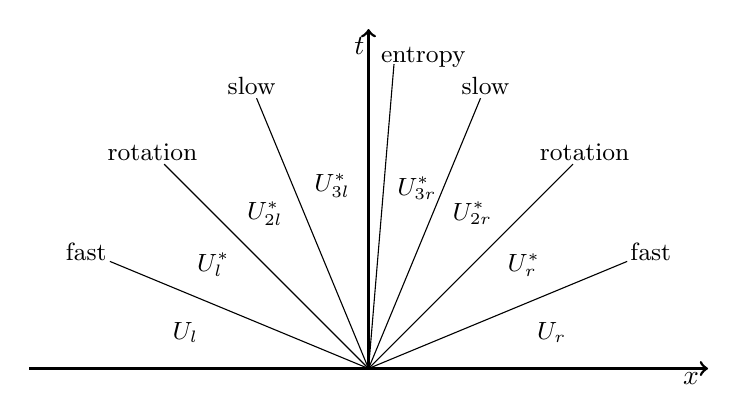
\begin{tikzpicture}[scale = {0.0125\linewidth},inner sep = 1pt]
%% \begin{tikzpicture}[scale = {0.015\linewidth},inner sep = 1pt]
%% \tikzstyle{every node} = [draw,circle,fill=gray!30];
%% \draw (-1.5,0.0) circle (0.8);
%% \draw[<->,line width=1pt] (0,1) node[right]{\;$t$}|-(1,0) node[below]{$m$};
\draw[line width=1pt] (0,0.95) node[left]{$t$}|-(0.95,0) node[below]{$x$};
\draw[->,line width=1pt] (0.95,0)--(1,0);
\draw[->,line width=1pt] (0,0.95)--(0,1);  
\draw[line width=1pt] (-0,0)--(-1,0);
\node[draw=white] (fr) at (0.83149,0.34442) {\small fast};
\node[draw=white] (rr) at (0.63640,0.63640) {\small rotation};
\node[draw=white] (sr) at (0.34442,0.83149) {\small slow};
%% \node[draw=white] (cd) at (0.17221,0.88337) {\small contact disc.};
\node[draw=white] (cd) at (0.16149,0.91587) {\small entropy};
\node[draw=white] (sl) at (-0.34442,0.83149) {\small slow};
\node[draw=white] (rl) at (-0.63640,0.63640) {\small rotation};
\node[draw=white] (fl) at (-0.83149,0.34442) {\small fast};

\node[draw=white] (R8a) at (0.53943,0.10730) {\small $\mbf{U}_{r}$};
\node[draw=white] (R7a) at (0.45731,0.30556) {\small $\mbf{U}^*_{r}$};
\node[draw=white] (R6a) at (0.30556,0.45731) {\small $\mbf{U}^*_{2r}$};
\node[draw=white] (R5a) at (0.14235,0.53126) {\small $\mbf{U}^*_{3r}$};
\node[draw=white] (R4a) at (-0.10730,0.53943) {\small $\mbf{U}^*_{3l}$};
\node[draw=white] (R3a) at (-0.30556,0.45731) {\small $\mbf{U}^*_{2l}$};
\node[draw=white] (R2a) at (-0.45731,0.30556) {\small $\mbf{U}^*_{l}$};
\node[draw=white] (R1a) at (-0.53943,0.10730) {\small $\mbf{U}_{l}$};

%% \node[] at (0.15,0.95) {contact};
\draw (0,0) -- (fr);  
\draw (0,0) -- (rr);  
\draw (0,0) -- (sr);  
\draw (0,0) -- (0.075,0.89678);  
\draw (0,0) -- (sl);  
\draw (0,0) -- (rl);  
\draw (0,0) -- (fl);  
\end{tikzpicture}

\end{center}
\caption{Seven possible waves and/or discontinuities separating the eight possible regions, or states of the ideal MHD Riemann problem.  The initial contact discontinuity, i.e., the entropy wave, separates regions $\mbf{U}^*_{3l}$ and $\mbf{U}^*_{3r}$.}
\label{fig:mhd_states}
\end{figure}

The exact solutions are composed of eight possible MHD states separated by seven wave fronts, as depicted in Figure \ref{fig:mhd_states}.  The transitions from one region to another through a discontinuity is controlled by the jump conditions associated with the discontinuity.  The Rankine-Hugoniot jump conditions for ideal MHD in Lagrangian mass coordinates, $dm = \rho dx$, are 
\begin{align} 
\label{eqn:jump1} W[V] &= -[v_n], \\ 
\label{eqn:jump2} W[v_n] &= -[P - B_n^2], \\
\label{eqn:jump3} W[\mbf{v}_{t}] &= -B_n[\mbf{B}_{t}], \\
%% \label{eqn:jump4} W[v_z] &= -B_x[B_z], \\
\label{eqn:jump5} W[V\mbf{B}_{t}] &= -B_n[\mbf{v}_{t}], \text{ and}\\
%% \label{eqn:jump6} W[VB_z] &= -B_x[v_z],   \\
\label{eqn:jump7} W[VE] &= [v_nP] - B_n[B_nv_n + \mbf{B}_{t}\cdot\mbf{v}_{t}],
\end{align}
where $P = p_g + \frac{1}{2}(B_n^2 + B_{t}^2)$ is the total pressure and $W = -(\rho v_n)_u = -(\rho v_n)_d$ is the Lagrangian velocity of the discontinuity and $V = 1/\rho$ \citep{Dai:1994a,Ryu:1995a}.  When moving in the $-x$ direction, the velocity $W$ is negative. Brackets are used to denote the difference between the upstream and downstream states for a quantity $Q$, i.e $[Q] = Q_u - Q_d$.  

\citet{Dai:1994a} give the fast and slow shock speeds in mass coordinates as
\begin{equation}
\label{eqn:speed_fs} W_{f,s}^2 = \frac{1}{2(1 + S_0)}\left[(C_s^2 + C_f^2 + S_1^2) \pm \sqrt{(C_s^2 + C_f^2 + S_1^2)^2 - 4(1 + S_0)(C_s^2C_f^2 - S_2)}\right],
\end{equation}
where $C_f = \rho c_f$ and $C_s = \rho c_s$.  The quantities $S_0, S_1, S_2$ are given by \citet{Ryu:1995a} in terms of $B_{t}$ as
\begin{align}
\label{eqn:speed_coef1} S_0 &= -\half (\gamma - 1)\frac{[B_{t}]}{B_{t}}, \\
\begin{split}
\label{eqn:speed_coef2} S_1 &= \half \left\{ -(\gamma - 2) V C_{t}^2 \frac{[B_{t}]}{B_{t}} + 2C_0^2 - (\gamma - 4) V C_{t}^2 \right. \\
& \;\;\;\; - \left. 2\gamma C_a^2 \vphantom{\frac{[B_{t}]}{B_{t}}} \right\} \frac{[B_{t}]}{B_{t}}\text{, and} 
\end{split} \\
\begin{split}
\label{eqn:speed_coef3} S_2 &= \half \left\{ \frac{C_a^2 [B_{t}]^2}{V} + (\gamma + 2)C_{t}C_a^2[B_{t}] + VC_{t}^2C_a^2(\gamma + 1) \right.\\
& \;\;\;\; + \left.(\gamma + 1)C_a^4  - 2C_0^2C_a^2 \vphantom{\frac{C_a^2 [B_{t}]^2}{V}}\right\} \frac{[B_{t}]}{B_{t}}, 
\end{split}
\end{align}
where $C_0 = \rho a$ is the Lagrangian speed of sound, $C_a = \rho c_a$ is the Lagrangian Alfv{\'e}n speed, and $C_{t} = \sqrt{\rho B_{t}^2}$.  The quantities in equations \eqref{eqn:speed_coef1}-\eqref{eqn:speed_coef3} are for the state downstream of the shock.

The relationships for fast rarefactions given by \citet{Ryu:1995a} are 
\begin{gather}
\label{eqn:rarefaction1} \dd{C_0}{B_{t}} = -\frac{\gamma + 1}{2} \sqrt{\rho} \frac{C_{t}C_s^2}{C_0(C_s^2 - C_a^2)} = \frac{\gamma + 1}{2} \sqrt{\rho} \frac{C_s^2(C_f^2 - C_a^2)}{C_a^2C_{t}C_0} = \frac{\gamma + 1}{2} \frac{\rho}{C_0} \dd{p_g}{B_{t}}, \\
\label{eqn:rarefaction2} \dd{v_n}{B_{t}} = \mp \frac{1}{\sqrt{\rho}} \frac{C_{\perp}C_a^2}{C_f(C_s^2 - C_a^2)} = \pm \frac{C_f^2 - C_a^2}{\sqrt{\rho} C_{t}C_f} = \pm\frac{2}{\gamma + 1} \frac{C_0C_a^2}{C_s^2C_f}\frac{1}{\rho} \dd{C_0}{B_{t}}\text{, and} \\
\label{eqn:rarefaction3} \frac{1}{\cos{\psi}} \dd{v_{t1}}{B_{t}} = \frac{1}{\sin{\psi}} \dd{v_{t2}}{B_{t}} = \mp \frac{1}{\sqrt{\rho}} \frac{C_a}{C_f},
\end{gather}
where the upper and lower signs refer to right- and left-going waves, respectively.  The rotation angle is defined by $\tan{\psi} = B_z/B_y$.

For slow rarefactions, replace the fast speed ($C_f$) with the slow speed ($C_s$) and the slow speed ($C_s$) with the fast speed ($C_f$) in Equations~\eqref{eqn:rarefaction1}-\eqref{eqn:rarefaction3}.  

An initial guess for the solution in the six interior regions shown in Figure~\ref{fig:mhd_states} is improved iteratively until the jump conditions of the initial contact or tangential discontinuity are satisfied to within a desired accuracy.  We have found a very high rate of convergence using the intermediate states approximated using the HLLD method for the initial guess. In practice, we use a relaxation factor and apply damping to speed up convergence. 

%-----------------------------------------------------------------
% HLLD approximate Riemann solver
%-----------------------------------------------------------------
\subsection[HLLD approximate Riemann solver]{HLLD approximate Riemann solver}
\label{sec:hlld}

%-----------------------------------------------------------------
% HLLD Riemann states
%-----------------------------------------------------------------
\begin{figure}[htbp]
\begin{center}
\tikzsetnextfilename{hlld_rstates}
%----------------------------------------------------------------------------------------
% hlld_rstates.tex
%----------------------------------------------------------------------------------------

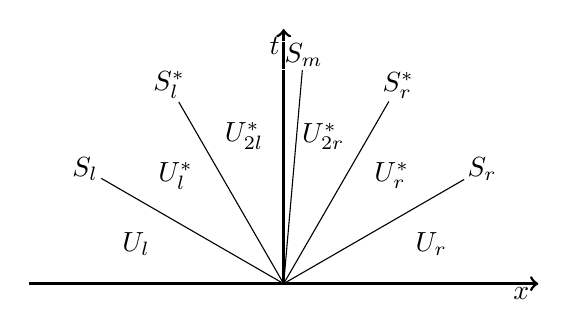
\begin{tikzpicture}[scale = {0.0125\linewidth},inner sep = 1pt]
%% \begin{tikzpicture}[scale = {0.015\linewidth},inner sep = 1pt]
%% \tikzstyle{every node} = [draw,circle,fill=gray!30];
%% \draw (-1.5,0.0) circle (0.8);
%% \draw[<->,line width=1pt] (0,1) node[right]{\;$t$}|-(1,0) node[below]{$m$};
\draw[line width=1pt] (0,0.7) node[left]{$t$}|-(0.7,0) node[below]{$x$};
\draw[->,line width=1pt] (0.7,0)--(0.75,0);
\draw[->,line width=1pt] (0,0.7)--(0,0.75);  
\draw[line width=1pt] (-0,0)--(-0.75,0);
\node[draw=white] (sr) at (0.58457,0.33750) {$S_r$};
\node[draw=white] (ssr) at (0.33750,0.58457) {$S^*_r$};
\node[draw=white] (cd) at (0.058830,0.67243) {$S_m$};
\node[draw=white] (ssl) at (-0.33750,0.58457) {$S^*_l$};
\node[draw=white] (sl) at (-0.58457,0.33750) {$S_l$};

\node[draw=white] (ur) at (0.43467,0.11647) {$\mbf{U}_{r}$};
\node[draw=white] (usl) at (0.31820,0.31820) {$\mbf{U}^*_{r}$};
\node[draw=white] (usr) at (0.11647,0.43467) {$\mbf{U}^*_{2r}$};
\node[draw=white] (usr) at (-0.11647,0.43467) {$\mbf{U}^*_{2l}$};
\node[draw=white] (usl) at (-0.31820,0.31820) {$\mbf{U}^*_{l}$};
\node[draw=white] (ul) at (-0.43467,0.11647) {$\mbf{U}_{l}$};

\draw (0,0) -- (sr);  
\draw (0,0) -- (ssr);  
\draw (0,0) -- (cd);  
\draw (0,0) -- (ssl);  
\draw (0,0) -- (sl);  

\end{tikzpicture}

\end{center}
\caption{Intermediate states and waves used in the HLLD approximate Riemann solver.}
\label{fig:hlld_rstates}
\end{figure}

An MHD extension of the HLLC scheme for the Euler equations (see Section~\ref{sec:hllc}) capable of resolving all isolated linear discontinuities of ideal MHD, i.e. RDs and CDs was developed by \citet{Miyoshi:2005}.  They referred to the scheme as HLLD, where the D stands for \emph{discontinuities}.  The HLLD scheme assumes a six-state solution separated by five waves as depicted in Figure~\ref{fig:hlld_rstates}.  Two nonlinear waves, i.e., shocks and rarefactions, separate the left and right initial states from the intermediate states in the Riemann fan, i.e., $\mbf{U}_{l}^*$, $\mbf{U}_{2l}^*$, $\mbf{U}_{2r}^*$, and $\mbf{U}_{r}^*$.  The four intermediate states are separated by two RDs with velocities, $S^*_l$, $S^*_r$, and one CD with velocity, $S_m$.  The one-dimensional wave speeds and intermediate states of \citep{Miyoshi:2005} have been modified for general coordinates, with $v_n = \mbf{v}\cdot\mbf{n}$, and $B_n = \mbf{B}\cdot\mbf{n}$, where  \mbf{n} is a normal vector with unit length.  

The velocity of the CD, $S_m$, is estimated with the HLL average given by \eqref{eqn:wave_spd_batten}, except gas pressure, $p_g$, is replaced with total pressure, $p_t$, and it becomes  
\begin{gather}
\label{eqn:hlld_sm}
S_m = \frac{(S_r - \vnr)\rho_r \vnr - (S_l - \vnl)\rho_l \vnl - p_{tr} + p_{tl} }
{(S_r - \vnr)\rho_r  - (S_l - \vnl)\rho_l}.
\end{gather}     
The intermediate states are approximated by solving the jump conditions across each wave.  Since the total pressure is conserved across the linear discontinuities in ideal MHD, the total pressure is constant throughout the Riemann fan.  It is given as 
\begin{gather}
\label{eqn:ptlr}
p_{t}^* = p_{tj}^* = p_{tj} + \rho_j (S_j - v_{nj})(S_m - v_{nj})
\end{gather}
for $j=l$ or $j=r$.  Substituting \eqref{eqn:hlld_sm} into \eqref{eqn:ptlr} and taking the averaging over the left and right states yields the explicit expression for total pressure throughout the Riemann fan:
\begin{gather}
\label{eqn:hlld_pt1}
p^*_{t} = \frac{(S_r - \vnr)\rho_r p_{tl} - (S_l - \vnl)\rho_l p_{tr} 
          + \rho_r\rho_l(S_r - \vnr)(S_l - \vnl)(\vnr - \vnl)}{(S_r - \vnr)\rho_r - (S_l - \vnl)\rho_l}.
\end{gather} 
 The states downstream of the fast waves, $\mbf{U}^*_j$ for $j=l$ and $j=r$ of Figure~\ref{fig:hlld_rstates}, are given in one-dimension by Eqs (41)-(47) of \citep{Miyoshi:2005}, written for general coordinates: they are
\begin{gather}
\label{eqn:hlld_d1}
\rho^*_j = \rho_j \frac{S_j - v_{nj}}{S_j - S_m} , \\
\label{eqn:hlld_v1}
\mbf{v}^*_{j} = \mbf{v}_{j} + \frac{\left(S_j - S_m\right)\left(p_{t}^* - p_{tj}\right)\mbf{n} 
  - B_n\mbf{B}_{j} \left(S_m - v_{nj}\right) }
               {\rho_j(S_j - v_{nj})(S_j - S_m) - B_n^2} , \\
\label{eqn:hlld_b1}
\mbf{B}^*_{j} = \frac{\mbf{B}_{j} \left(\rho_j(S_j - v_{nj})^2 - B_n^2\right) 
  - B_n\left(p_{t}^* - p_{tj}\right)\mbf{n}}
                {\rho_j(S_j - v_{nj})(S_j - S_m) - B_n^2} , \\
\label{eqn:hlld_en1}
E^*_j = \frac{(S_j - v_{nj})E_j - p_{tj}v_{nj} + p^*_{t}S_m + B_n(\mbf{v}_{j}\cdot\mbf{B}_{j} 
        - \mbf{v}^*_{j}\cdot\mbf{B}^*_{j})}{S_j - S_m} .
\end{gather}
If $\mbf{n} = (1,0,0)$, $v_x = S_m$, $B_x = B_n$, \eqref{eqn:hlld_v1} and \eqref{eqn:hlld_b1} reduce to (44)-(47) of \citep{Miyoshi:2005}, given as  
\begin{gather*}
v^*_{yj} = v_{yj} -B_x B_{yj} \frac{S_m - v_{nj} }
               {\rho_j(S_j - v_{nj})(S_j - S_m) - B_x^2} , \\
v^*_{zj} = v_{zj} - B_x B_{zj} \frac{S_m - v_{nj} }
               {\rho_j(S_j - v_{nj})(S_j - S_m) - B_x^2} , \\
B^*_{yj} = B_{yj} \frac{\rho_j(S_j - v_{nj})^2 - B_x^2} 
                {\rho_j(S_j - v_{nj})(S_j - S_m) - B_x^2} , \text{ and }\\
B^*_{zj} = B_{zj} \frac{ \rho_j(S_j - v_{nj})^2 - B_x^2} 
                {\rho_j(S_j - v_{nj})(S_j - S_m) - B_x^2}. 
\end{gather*}

The states downstream of the rotational discontinuity, $\mbf{U}^*_{2j}$, of Figure~\ref{fig:hlld_rstates}, can be found in terms of the initial left state and $\mbf{U}^*_j$.  The density, normal velocity, and total pressure are 
\begin{gather}
\label{eqn:hlld_d2}
\rho^*_{2j} = \rho^*_j , \\
\label{eqn:hlld_vn2}
v^*_{n2j} = v^*_{nj} , \\
\label{eqn:hlld_pt2}
p^*_{t2j} = p^*_{tj} ,
\end{gather}
because they are constant across the rotational discontinuity.  The Alfv{\'e}n speeds of the left and right rotational discontinuities are    
\begin{gather}
\label{eqn:hlld_rd_spd}
S^*_l = S_l - \frac{|B_n|}{\sqrt{\rho^*_l}} \text{ and}\;\;\;\; S^*_r = S_r + \frac{|B_n|}{\sqrt{\rho^*_r}}. 
\end{gather}
The description of the HLLD intermediate states is completed by solving for $\mbf{v}^*_{m} = \mbf{v}^*_{2l} = \mbf{v}^*_{2r}$ and $\mbf{B}^*_{m} = \mbf{B}^*_{2l} = \mbf{B}^*_{2r}$.  This is done using the integral conversation law over the Riemann fan $(S_l \delta t, S_r \delta t) \times (0, \delta t)$ (Eq. (58) of \citep{Miyoshi:2005}).  They are given as  
\begin{gather}
\label{eqn:hlld_vt2}
\mbf{v}^*_{m} = \frac{\sqrt{\rho^*_l}\vnl^* + \sqrt{\rho^*_r}\vnr^* + (\mbf{B}_r^* - \mbf{B}_l^*)\text{sign}(B_n)}
                {\sqrt{\rho^*_l} + \sqrt{\rho^*_r}} , \\               
\label{eqn:hlld_bt2}
\mbf{B}^*_{m} = = \frac{\sqrt{\rho^*_l}\mbf{B}_r^* + \sqrt{\rho^*_r}\mbf{B}_l^* 
                + \sqrt{\rho^*_l\rho^*_r}(\mbf{v}_r^* - \mbf{v}_l^*)\text{sign}(B_n)}
                {\sqrt{\rho^*_l} + \sqrt{\rho^*_r}} \text{, and}\\               
\label{eqn:hlld_en2}
E^*_{2j} = E^*_j \mp  \sqrt{\rho^*_j}(\mbf{v}^*_{j}\cdot\mbf{B}^*_{j} 
        - \mbf{v}^*_{2j}\cdot\mbf{B}^*_{2j})\text{sign}(B_n) ,
\end{gather}
where the minus (plus) sign corresponds to $j=l$ ($j=r$).  The HLLD fluxes are found by applying the integral conservation laws over the left half or right half of the Riemann fan, $(S_l\delta t, 0)\times (0,\delta t)$ or $(0,S_r\delta t)\times (0,\delta t)$, see Appendix~\ref{app:hll_flux}.  The fluxes are given as
\begin{gather}
\label{eqn:hlld_flux}
\mbf{F}(x,t) = 
\begin{cases}
\mbf{F}_l   \phantom{= \mbf{F}_l  + S_l (\mbf{U_l^*} - \mbf{U_l}} & \text{if}\;\;\; 0 < S_l, \\
\mbf{F}_l^* = \mbf{F}_l  + S_l (\mbf{U}_l^* - \mbf{U}_l) & \text{if}\;\;\; S_l \le 0 \le S^*_l, \\
\mbf{F}_{2l}^* = \mbf{F}^*_l  + S^*_l (\mbf{U}_{2l}^* - \mbf{U}^*_l) & \text{if}\;\;\; S^*_l \le 0 \le S_m, \\
\mbf{F}_{2r}^* = \mbf{F}^*_r  + S^*_r (\mbf{U}_{2r}^* - \mbf{U}^*_r)  & \text{if}\;\;\; S_m \le 0 \le S^*_r, \\
\mbf{F}_r^* = \mbf{F}_r  + S_r (\mbf{U}_r^* - \mbf{U}_r)  & \text{if}\;\;\; S^*_r \le 0 \le S_r, \\
\mbf{F}_r  \phantom{= \mbf{F}_r  + S_r (\mbf{U_r^*} - \mbf{U_r}} & \text{if}\;\;\; S_r < 0. \\
\end{cases}
\end{gather}

The HLLD method is robust because it is positivity preserving and it is less computationally expensive than schemes such as Roe's that require eigenvalue decomposition.  Results from MHD shock tube problems solved using the HLLD fluxes are given in Sections~\ref{sec:riemann_mhd}-\ref{sec:nonuniform_converge}.  However, scheme produces compound waves for coplanar and near coplanar cases as demonstrated in Sections~\ref{sec:riemann_mhd}-\ref{sec:nonuniform_converge}, an issue all approximate Riemann solvers suffer from.  In Chapter \ref{chp:cwm}, a modification to the HLLD fluxes that removes compound waves from the solution to coplanar and near coplanar Riemann problems of ideal is described.  
